
%Anders version:
%\documentclass[11pt]{article}
%\renewcommand{\baselinestretch}{1.4}

\documentclass[final,pdftex]{Oskarthesis}
\usepackage[dvipsnames,cmyk]{xcolor}
\usepackage{etex} %Must be first!
\usepackage{geometry}
\usepackage{lmodern}

\usepackage{algorithmicx}
\usepackage{algpseudocode}
\usepackage{algorithm}

%\documentclass[a4paper,12pt]{article}
%\usepackage{etex} %Must be first!
\usepackage[font=footnotesize, margin=1cm]{caption}
\usepackage[swedish,english]{babel}

%\usepackage[garamondx,cmbraces]{newtxmath}

%\usepackage[erewhon,vvarbb,bigdelims]{newtxmath}
\usepackage[T1]{fontenc}
\usepackage{mathtools}


\usepackage[utf8]{inputenc} % set input encoding (not needed with XeLaTeX)

\usepackage{nomencl}
%\usepackage[bw]{mcode}
%\usepackage[latin1]{inputenc}
\usepackage[colorlinks]{hyperref}
\usepackage{booktabs} %Nice tabular
\usepackage{marvosym}
\usepackage[dvipsnames]{xcolor}
\usepackage{xspace}
\hypersetup{
    unicode=false,          % non-Latin characters in Acrobat’s bookmarks
    pdftoolbar=true,        % show Acrobat’s toolbar?
    pdfmenubar=true,        % show Acrobat’s menu?
    pdffitwindow=false,     % window fit to page when opened
    pdfstartview={FitH},    % fits the width of the page to the window
    pdftitle={},    % title
    pdfauthor={Oskar B. V\"astberg},     % author
    pdfsubject={},   % subject of the document
    pdfnewwindow=true,      % links in new window
    colorlinks=true,       % false: boxed links; true: colored links
    linkcolor=black,          % color of internal links
    citecolor=black,        % color of links to bibliography
    filecolor=black,      % color of file links
    urlcolor=black           % color of external links
}
\usepackage{listings, courier}
\usepackage{float}
\usepackage{amssymb, graphicx, fancyhdr}
%\usepackage{units}
\usepackage{amsmath}
\numberwithin{equation}{section}
\usepackage{amsthm}
\usepackage{mathrsfs} %To get P from mathscr
\usepackage{subfig}
\usepackage{multirow}
\usepackage{caption}
\usepackage{natbib, hypernat}
\usepackage{apalike}
\usepackage{paralist} %for inline lists!
\usepackage{enumitem}
\usepackage{lscape}

% Make it possible to force floats to occur before a specific point
\usepackage{placeins}

%for tikz pictures ---------\textemdash-
\usepackage{tikz,pgfplots}
\usetikzlibrary{decorations}
\usetikzlibrary{calc,shapes,arrows}

\tikzset{
	font={\fontsize{8pt}{12}\selectfont}}

\pgfplotsset{compat=newest} %for plots
\pgfplotsset{plot coordinates/math parser=false} %and for speed

%%ONLY WORKINPROGRESS%%%%%%%%%%%%%%%%
%\usepackage{showlabels}
%\usepackage{pifont} % Use to create funny things in todo list :)	
\usepackage{bbm}

\newcommand{\indicator}[1]
{\mathbbm{1}_{#1}}
\newcommand{\ks}[1]{^{(#1)}}

%------------------------------------ Set new commands ---------

%%%%%% General %%%%%%%%%%%%%%%%%%%%
\newcommand{\ve}[1] %make vector notation
{{\bf #1}}

\newcommand{\unit}[1] %Units
{\, \mathrm{#1}}
\newcommand{\units}[1] %Units
{\, \mathrm{#1}}
\newcommand{\Bl} % Big left
{{\Big ( }}
\newcommand{\bl} % Big left
{{\big ( }}

\newcommand{\Bh} % Big left
{{\Big ) }}
\newcommand{\bh} % Big left
{{\big ) }} 


%%%%%% Theorems %%%%%%%%%%%%%%%%%%
\usepackage{amsmath}               
  {
      \theoremstyle{plain}
      \newtheorem{assumption}{Assumption}
  }
\usepackage{amsmath}               
  {
      \theoremstyle{plain}
      \newtheorem{theorem}{Theorem}
  }
  
  \usepackage{amsmath}               
  {
  	\theoremstyle{plain}
  	\newtheorem{lemma}{Lemma}
  }
\newcommand{\refas}[1]
{A(\ref{#1})}

%%%%%% Mathematics %%%%%%%%%%%%%%%%%%
\newcommand{\abs}[1]{\lvert#1\rvert} %Abs
\newcommand{\norm}[1]{\lVert#1\rVert} %Norm

%Case 
\newcommand{\cif}  %If in cases
{\text{ if }}

\newcommand{\celse}  %If in cases
{\text{ else}}

%Partial derivatives
\newcommand{\dxdy}[2] %make a dx/dy with d as normally done
{\frac{\text{d}#1}{\text{d}#2}}

\newcommand{\ddxdy}[2] %make a dx/dy with d as normally done
{\frac{\partial \, #1}{\partial#2}}




\newcommand{\dx}[1] %make a dx
{{\Delta#1}}

\newcommand{\ud}{\,\mathrm{d}} %make nice dx in integral

\newcommand{\dder}[2] %discrete derivate notation
{ #2^* }
%Other
\newcommand{\nint}[1]
{\text{nint} \, #1}
\newcommand{\bsigma}
{\bold{\sigma}}
\newcommand{\lse}[1]
{\mathrm{lse} \, #1}

\DeclareMathOperator*{\argmax}{arg\,max}

%\newcommand{\unit}[1] %make vector notation
%{\, \mathrm{#1}}


%%%%% Notations for estimation%%%%%%%
\newcommand{\Ll} % Likelihood notation
{\mathscr{L}}
\newcommand{\LL} % Log-likelihood notation
{\mathscr{LL}}
\newcommand{\pp} % Probability
{\mathscr{P}}
\newcommand{\obs} % Observation set
{\mathscr{O}}

%%%% Dynp %%%%%%%%%%%
% General dynp notations
\newcommand{\EV} % Expected utility notation
{\eutil}
% Notations for state spaces in dynp
\newcommand{\Cc} %Write choice set
{\mathbb{C}}
\newcommand{\Ccsamp}
{\tilde{\Cc}}
\newcommand{\Uu} %write U set
{\mathbb{U}}
\newcommand{\xx} %write x set
{\mathbb{X}}
\newcommand{\uu} % write u set
{\mathbb{U}}
\newcommand{\rr} % write R set
{\mathbb{R}}
\newcommand{\Agood} % write action-sequence set
{\mathscr{A}}
\newcommand{\seqspace} % Write statespace
{\mathscr{S}}
\newcommand{\eutil} % Expected utility notation
{\ensuremath{EV}}
\newcommand{\ev} % Expected utility notation
{\ensuremath{\bar{V}}}
\newcommand{\param}[1]
{{\ensuremath{\theta_{\text{#1}}}\xspace}}
\newcommand{\laeutil} % Expected utility notation
{\ensuremath{\overline{\eutil}}\xspace}
\newcommand{\aeutil} % Expected utility notation
{\ensuremath{\widetilde{\eutil}}\xspace}


\newcommand{\med}[1]
{ \bar{#1}}

\newcommand{\TB}{T_{\beta}}
%FOR TIKZ%%%%%%%%%%%%%%%%%%%%%%%%%%%%%%%%%%%%
\usepackage{tikz}
\usetikzlibrary{decorations.markings}
\usetikzlibrary{shapes.geometric}

\pgfdeclarelayer{edgelayer}
\pgfdeclarelayer{nodelayer}
\pgfsetlayers{edgelayer,nodelayer,main}

\tikzstyle{none}=[inner sep=0pt]
\tikzstyle{rn}=[circle,fill=blue!40,draw=black,line width=0.8 pt]
\tikzstyle{gn}=[circle,fill=yellow!40,draw=black,line width=0.8 pt]
\tikzstyle{yn}=[circle,fill=red!40,draw=black,line width=0.8 pt]
\tikzstyle{rnn}=[circle,fill=blue!40,draw=black,line width=0.3 pt,inner sep=0pt, minimum size=0.10cm]
\tikzstyle{gnn}=[circle,fill=yellow!40,draw=black,line width=0.3pt,inner sep=0pt, minimum size=0.10cm]
\tikzstyle{ynn}=[circle,fill=red!40,draw=black,line width=0.3 pt,inner sep=0pt, minimum size=0.10cm]
\tikzstyle{enn}=[circle,fill=black!40,draw=black,line width=0.3 pt,inner sep=0pt, minimum size=0.10cm]
\tikzstyle{wn}=[circle,fill=white,draw=black,line width=0.8 pt]
\tikzstyle{simple}=[->,dashed,draw=black!80,line width=0.400]
\tikzstyle{arrow}=[->,draw=black,line width=1.000]
\tikzstyle{tick}=[-,draw=black, line width = 0.6]
\tikzstyle{simpleSmall}=[->,dashed,draw=black!80,line width=0.100]
\tikzstyle{arrowSmall}=[->,draw=black!80,line width=0.2000]
\tikzstyle{arrowMedium}=[->,draw=black,line width=0.4000]
\tikzstyle{arrowTiny}=[->,draw=black!30,line width=0.1000]
\tikzstyle{tickSmall}=[-,draw=black, line width = 0.2]
\tikzstyle{block} = [draw=white, fill=white!20, rectangle,text centered,opacity=0,text opacity = 1,font=\scriptsize ]
\tikzstyle{onlytext}=[block,text width=1.5cm]






\newcommand{\act}[1]{\tilde{#1}}
\newcommand{\amem}{h}
\newcommand{\atime}{\tau}
\newcommand{\zdel }{\,}

\newcommand{\footremember}[2]{%
   \footnote{#2}
    \newcounter{#1}
    \setcounter{#1}{\value{footnote}}%
}
\newcommand{\footrecall}[1]{%
    \footnotemark[\value{#1}]%
} 

\begin{document}
\begin{frontmatter}
	\title{A dynamic discrete choice activity based travel demand model}
	\runtitle{A DDCM of travel demand}
	
	
	\begin{aug}
		\author{\fnms{Oskar} \snm{Blom V\"astberg}\ead[label=e1]{oskar.vastberg@abe.kth.se}}
		\author{\fnms{Anders} \snm{Karlstr\"om}}
		\author{\fnms{Daniel} \snm{Jonsson}}
		\author{\fnms{Marcus} \snm{Sundberg}}
		\vspace{0.2cm}
		
		{\centering \footnotesize\emph{KTH Royal Institute of Technology, SE-100 44 Stockholm, Sweden}}
		
		\runauthor{O. B. V\"astberg et. al.}
		
		\address{Corresponding author: \printead{e1}}

	\end{aug}
	\def\abstractname{}
	\begin{abstract}
During the last decades, many activity-based models have been developed in the literature. However, especially in random utility based models timing decisions are often treated poorly or inconsistently with other choice dimensions. In this paper we show how dynamic discrete choice can be used to overcome this problem. In the proposed model, trip decisions are made sequentially in time, starting at home in the morning and ending at home in the evening. At each decision stage, the utility of an alternative is the sum of the one-stage utility of the action and the expected future utility in the reached state.

The model generates full daily activity schedules with any number of trips that each is a combination of one of 6 activities, 1240 locations and 4 modes. The ability to go from all to all locations makes evaluating the model very time consuming and sampling of alternatives were therefore used for estimation. The model is estimated on travel diaries and simulation results indicates that it is able to reproduce timing decisions, trip lengths and distribution of the number trips within sample. 

To explain when people perform different activities, two sets of parameters are used: firstly, the utility of being at home varies depending on the time of day; and secondly, constants determine the utility of arriving to work at specific times. This was enough to also obtain a good distribution of the starting times for free-time activities. 

	\end{abstract}
\end{frontmatter}
\section{test}
%1 : Why ABM?


Travel demand models have during the last decades evolved from highly aggregated trip based models, through tour based models into activity based models that considers the choice of full daily activity-travel patterns including all activities and all transportation at an individual or household level. Activity based models sets out to model the interdependence of all activity-travel episodes performed during the day as trips are naturally linked in space-time. As demand for travel is derived from the demand for activity participation, demand for activities should be a determinant for if, when and where trips are being performed. Modelling the interdependence of all aspects of an activity-travel pattern together with time-space constraints is especially important when considering policy changes such as congestion charge that are becoming increasingly important in today's traffic planning, as how people react to such policies depend on how they trade-off between, e.g., arrival time to work, cost and mode of transport. 

To achieve an interdependent choice a full daily travel pattern, it is common to assume that individuals (or households) make the decision of how to plan their day based on some sort of scoring or utility function including all activity and travel episodes of the day. Possible the first model based on this assumption was presented by \citet{Adler79}, who assumed that individuals behaved as if they choose the utility maximising travel pattern among the set of all feasible travel patterns.
To actually implement a model based on this assumption in 1979 they had to impose some additional restrictions: firstly the choice set was limited to observed travel patterns; and secondly timing of trips were not modelled. One of the great challenges with implementing a model for the choice of a full activity-travel pattern is still the immense size of the choice set, especially when timing of trips are considered. Alternatives methods that does not require choice set formation has therefore been developed. In the Household Activity Pattern Problem (HAPP), the choice of all household members daily travel patterns including time-of-day, mode and location choices is formulated as constrained mixed-integer optimisation problem \citep{recker2001bridge,Recker08,Recker13,yuan2014HAPP}. The problem is solvable, but computationally very demanding and with only 19 locations the computation time is reported to an average of $614\units{s/household}$ \citep{Recker13}. The choice of an activity-travel pattern can also be formulated as a shortest-path problem in a an abstract network, as in the multistate-supernetwork model \citep{arentze04Multistate}. In such a network, states can be defined for remaining mandatory activites and thus capture time-space constraints \citep{liao2013incorporating,liao2016modeling}. Similarly to HAPP, the computation time is still a limiting factor. \citet{liao2016modeling} reports that the evaluating the choice of a daily travel pattern takes $8\units{s}$ when an individual has two fixed activities to perform in a day and 6 locations to choose from.
%It is further not yet clear how to estimate the model, as parameters currently are obtained by using separate MNL models for different choice dimensions in \citet{Liao2017}. The model estimated is thus not identical with the shortest path problem solved when the model is used for simulation in, e.g., \citet{liao2016modeling}.

Some models, e.g.,  Starchild \citep{recker86starchild1,recker86starchild2}, have avoided the need to formulate the universal choice set by constructing a random process by which alternative travel patterns are derived, and compare a smaller set of alternative travel patterns obtained from this process based on their full utilities.  
A similar approach is also used in MATSim which besides mode, timing and location also include route choice for of all trips although the number of activities and their ordering is fixed  \citep{lefebvre2007fast,grether2009mode,balmer05,horni2012high}.  AMOS \citep{kitamura1996Sams} set out to mimic how individuals adapt their travel patterns in the event of changes to environment and evaluate whether the perturbations offer any improvement in terms of full daily utility. Somewhat similarly, AURORA focuses on how individuals reschedule a given set of activities by adjusting their activity-travel pattern until further adjustments does not motivate the search cost \citep{timmermans2001modeling,joh2003Aurora, johEstimationAurora2005}.

An alternative to consider the choice of a full daily travel pattern as a joint choice has been to model a sequential choice of, e.g., whether or not to perform a trip, departure time, mode of transport, destination and purpose. The probability to make a new choice is then modelled conditional on previous choices, and a sequence of choices will produce a daily travel pattern. This is the approach taken in, e.g., Albatross \citep{timmermans2001modeling} and CEMDAP \citep{bhat2004comprehensive}. In such sequential models, the full history can influence the probability in any choice situation, ensuring an interdependence between trips. \citet{Habib11RUM} developed a discrete-continuous random utility model for weekend travelling where agents decided on mode, destination and activity based on the utility of the combination. Agents in the model of \citet{Habib11RUM} also considered how their decisions influenced future opportunities by including a utility component for the value of future time. The value of future time was modelled as a time-of-day dependent composite good, which was parameterized and estimated. 

A sequential model where a part of the history influences the probability of choices at the current point in time can be interpreted as a Markov process. Some work on activity planning has been explicitly formulating Markov chains to analyse the sequential dependence of different activity purposes. \citet{AllahviranlooMDP13} models how the probability of a specific activity by estimating transition probabilities from one activity to another based on socio-demographics and the history of previously performed activities, formulated as a Markov chain. \citet{susilo2014repetitions} used a Markov chain to model how activities performed on one day influences activities performed on subsequent days. \citet{hasan18} used a Markov chain to model sequential choices of activities and location in order to infer missing information in geo-location data gathered from social media.  


%Since all aspects of a travel pattern is interconnected, it seems reasonable to assume that individuals evaluate the full pattern when determining what activities to engage in as well as timing, location and mode of transport. Assuming that individuals (or households) act as if the consider the utility of a full daily travel pattern is not a new idea. It was proposed in \citet{Adler79}, who base a model on the assumption that households make a joint choice of a travel pattern $tp$, considering travel time, mode and destination choices for all tours during a day by selecting the optimal pattern $tp^*$ from the set of feasible patterns $TP$ according to: $tp^* = \argmax_{tp \in TP} U(tp) + \epsilon_{tp}$. With $\epsilon_{tp}$ Gumble distributed, this becomes an MNL model which was estimated using the observed sample as a choice set. Individuals are also considering the full daily travel pattern in: \citet{Recker08}, who formulates the model as a mathematical programming problem; and in MATSim \citep{balmer05,horni2011} who uses simulation to obtain close too optimal solutions. In AURORA \citep{joh2003Aurora,johEstimationAurora2005}, individuals are considering the utility of the full daily travel pattern but are assumed to use search-heuristics to schedule (and reschedule) their day. 
%%2 : ABM so far 

% For a comprehensive overview of activity based models, see e.g., \citet{Pinjari11} or \citet{Rasouli14}. 


The standard practice in the field of travel demand modelling is based on random utility maximisation, and even more specifically nested logit. One of the most extensive such models to date was initially presented in \citet{bowman2001} where a nested logit structure is developed for the choice of all trips performed during a day. The model treats tours and activities sequentially based on their importance for the individual. The model consists of five nests: 1) the choice of activity pattern, including the number of tours carried out during the day; 2) the choice of time of day for the primary tour and all its trips; 3) the mode and destination for the primary tour; 4) the time of day for the secondary tours; and 5) the mode and destination of the secondary tours. The nested logit structure ensures that higher decisions, such as the choice of activity pattern, includes the individual specific information about all available tour-combinations that the pattern includes. Many extensions to the original prototype model presented in \citet{bowman2001} has since been performed, to, e.g., allow for a greater detail in time-of-day choice \citep{Vovsha04}. In a recent implementation, time-of-day is modelled at a 30 minute resolution, where each individual consider a sampled subset of possible 30-minute intervals for each trip \citep{bradley2010sacsim}. In a discrete choice framework, it is logical to use the expected (maximum) utility from a day-path as input to higher order models and for cost appraisal \citep{Geurs10}. The expected utility could also be used to get detailed disaggregated measures of accessibility \citep{dong2006moving}.


% The probability of choosing a tour that ends at 5 PM should depend on the expected utility of the rest of a day when being home at 5 PM. If one more tour is to be conducted during the remaining time of the day, then they can be started at 10 alternative times before 10 PM. For the secondary tour, taking place after 5 PM, the expected utility should in turn depend on the starting time, since that will influence the number of available destinations that can be reached, as well as the time that can be spent on different activities. It should also depend on when one is finished with all activities.

%and \citep{bhat04} 

Although a large number of travel demand models  have been developed in the past, no model has to date managed to model the interdependent choice of a full day with a detailed time dimension while remaining consistent with utility maximisation and while being reasonably computationally demanding. Individual rationality is to-date a corner stone for welfare economics, enabling the approach to be theoretically and consistently translated into a tool for cost-benefit analysis. We see this argument as difficult to ignore without having a theory for behavioural welfare economics in sight. Further, non of the models discussed accounts for travel time uncertainty. Even when their purpose is to model rescheduling as in \citet{joh2003Aurora}, they assume that people are unaware of the possible need to reschedule when they make their decisions. Travel time uncertainty has been observed to have an important impact on departure time decisions and has been extensively studied using scheduling models following \citet{small82scheduling}. On the other hand, scheduling models up-to-date typically considers a single trip in isolation \citep[as in, e.g.,][]{fosgerau10reliability}, or possibly a chain of two trips \citep{jenelius11tripchain}. They may therefore not be suitable to analyse the system wide effects of more reliable travel times. Incorporating planning under uncertainty in a travel demand model is therefore an important topic. 

This paper builds on the proposed dynamic discrete choice model presented in \citet{karlstrom04} which \citet{jonsson2014reconciling} illustrated could be used to obtain give detailed time-of-day dependent accessibility measures, as demonstrated by \citet{jonsson2014reconciling}. In this paper, we show how a Markov Decision Process can be formulated to model the choice of a daily activity-travel pattern. 

In Section 2 of this paper, we show how a Markov Decision Process (MDP) can be used to model the choice of a daily activity-travel pattern. Following the random utility maximising approach, we assume that individuals maximise the expected achieved utility from a path through activity-location-time-space throughout one day. In the presence of stochasticity, a utility-maximizing agent will derive a decision policy outlining how to act conditional on the outcome of the stochastic process. Such a policy could be interpreted as contingency plan, specifying which travel pattern to choose for each possible combination of outcomes of the stochastic process. This is in contrast to available models where utility-maximisation of a activity-travel pattern has been modelled, e.g., Starchild, MATSim, HAPP and the multistate-supernetwork. One can formulate the choice of an activity-travel pattern as a possible policy where the decisions are fixed before the day start. However, a policy and especially the optimal policy could in general not be defined as a travel pattern, as it does not necessarily contain a fixed set of decisions independently of what happens. 

%In an MDP these transition probabilities are dependent on the choices of a decision maker and the interest lies in inferring the control law guiding their decisions. This is in in contrast to the Markov chain models discussed above where the interest lies in obtaining transition probabilities conditional on a specific state.

In Section 3, we show how the MDP developed in Section 2 can be formulated as a Dynamic discrete choice model (DDCM) following the work by \citet{rust1987} and thereby give state dependent choice probabilities that are a function not only of the state but also on the expected future utility conditional on the chosen action. We discuss how the expected future utility, i.e., the value function can be approximated using linear interpolation when time is modelled as a continuous variable and when travel time is uncertain. Using the obtained value functions it is possible to calculate choice probabilities and thus potentially use maximum likelihood estimation. Following \citet{fosgerau2013}, we show how the model in a special case degenerates into an MNL model over sequences of actions, and thus can be estimated using sampling of alternatives. Estimates obtained using sampling of alternatives are in contrast to direct maximum likelihood estimates not sensitive to approximations used when calculating the value function.
While similar to the approach developed in \citet{Habib11RUM}, this expected future utility is not parameterized but instead obtained as the expectation of  future one-stage utilities ans is therefore sensitive to changes in the transportation system which only influence the future and so, e.g., the choice of departure time to work in the morning will therefore be sensitive to the traffic conditions in the afternoon. The DDCM approach taken in this paper closely follows the standard nested logit practice, but introduces time explicitly, respecting that time has a direction and that decisions in real-life actually can be made sequentially in time, given the information available at each point in time when a decision is made. 

Observe that by using a DDCM formulation, the optimal decision is obtained using backward induction where every possible state-action combination is traversed, a process that can be computationally very demanding when the number of such combinations is large. It may not seem behaviourally realistic that individuals actually solve this complicated problem. As noted by \citet{RustML88}, an adapation and learning algorithm may provide a better explanation of how people may find the optimal decision rule in an MDP and thus act \emph{as if} they were utility maximisers. It is possible to find an approximate solution to an MDP using reinforcement learning which it has been argued represent a good description of how people plan their days \citep[see, e.g.,][]{arentze2004learning}. MDP's of activity-scheduling has also been solved using reinforcement learning by \citet{vanhusel09} to model the sequential planning of activities. \citet{Feygin18} proposed in his thesis how the decision rules in MDP for activity scheduling can be estimated using inverse reinforcement learning. \citet{karlstromScalingUp2009} also investigated how a boltzmann machine can be used to solve an MDP of the type proposed in this paper. 

In section 4, we present a case study were a model over a working day is specified and estimated on a travel survey. The case study presented in this paper excludes travel time uncertainty, and focus on the special case that can be estimated using sampling of alternatives. By focusing on this special case, we are able to assess the effects of the value function approximation on aggregate predictions. Section 5 discuss the results and section 6 concludes and discuss future work.  



\section{Introduction}
%1 : Why ABM?
Travel demand models have during the last decades evolved from highly aggregated trip based models, through tour based models into activity based models that considers the choice of all activities and all transportation for a full day (or longer) at an individual (or household) level. The motivation behind this gradual increase in complexity is the realization that the demand for travel is derived from the demand for activity participation. Accurate predictions of how individuals will react to infrastructure investments and policy changes should therefore ideally take into account to what extent individuals are flexible in their activity participation. There is only a limited amount of time each day and some activities are more or less fixed in both location and time, such as working and picking up or dropping of children at school/daycare. These constraints severely restrict individuals' ability to adapt and not considering them is therefore likely to result in unrealistic forecasts. This is especially the case when considering policy changes such as congestion charge that are becoming increasingly important in today's traffic planning. 

A natural way to accomplish an interdependent choice of all aspects of a daily travelling would be to directly model the choice of a full daily travel pattern.
The problem with this approach is that the number of possible ways to plan a day is immense. One could definitely argue that people do not actually consider all these alternatives, but there are definitely complex aspects of the activity schedule that do influence how people plan their days. For example, when considering what time to leave for work, they are likely to take into consideration when they will get home and so the preferred departure time to work should be derived from a trade-off between time spent at home in the morning versus time spent at home (or on some activity) in the evening.

%Since all aspects of a travel pattern is interconnected, it seems reasonable to assume that individuals evaluate the full pattern when determining what activities to engage in as well as timing, location and mode of transport. Assuming that individuals (or households) act as if the consider the utility of a full daily travel pattern is not a new idea. It was proposed in \citet{Adler79}, who base a model on the assumption that households make a joint choice of a travel pattern $tp$, considering travel time, mode and destination choices for all tours during a day by selecting the optimal pattern $tp^*$ from the set of feasible patterns $TP$ according to: $tp^* = \argmax_{tp \in TP} U(tp) + \epsilon_{tp}$. With $\epsilon_{tp}$ Gumble distributed, this becomes an MNL model which was estimated using the observed sample as a choice set. Individuals are also considering the full daily travel pattern in: \citet{Recker08}, who formulates the model as a mathematical programming problem; and in MATSim \citep{balmer05,horni2011} who uses simulation to obtain close too optimal solutions. In AURORA \citep{joh2003Aurora,johEstimationAurora2005}, individuals are considering the utility of the full daily travel pattern but are assumed to use search-heuristics to schedule (and reschedule) their day. 
%%2 : ABM so far 
How to spend the limited time budget when the preferences for time is dependent on the time of day should be the key determinant for when, where and if people choose to conduct different activities in activity based models. Although many activity based models up to date result in full day activity schedules, most fall short in their treatment of time. For a comprehensive overview of activity based models, see e.g., \citet{Pinjari11} or \citet{Rasouli14}. As an extension to the tour-based approach, \citet{Bowman01} developed a nested-logit structure that treats tours and activities sequentially based on their importance for the individual. The model consists of five nests: 1) the choice of activity pattern, including the number of tours carried out during the day; 2) the choice of time of day for the primary tour and all its trips; 3) the mode and destination for the primary tour; 4) the time of day for the secondary tours; and 5) the mode and destination of the secondary tours. The nested-logit structure ensures that higher decisions, such as the choice of activity pattern, includes the individual specific information about all available tour-combinations that the pattern includes. However, since secondary tours are not conditioned on each other, they are not temporarily consistent. For instance, it is technically possible to end up with daily patterns that take more than a full day to complete. The model has been further developed by combining with a duration and departure time model, which is not integrated into the nested-logit structure \citep{Vovsha04,Bradley10} and so does not integrate upwards. 
% The probability of choosing a tour that ends at 5 PM should depend on the expected utility of the rest of a day when being home at 5 PM. If one more tour is to be conducted during the remaining time of the day, then they can be started at 10 alternative times before 10 PM. For the secondary tour, taking place after 5 PM, the expected utility should in turn depend on the starting time, since that will influence the number of available destinations that can be reached, as well as the time that can be spent on different activities. It should also depend on when one is finished with all activities.

There are a number of models in the literature that is related to the approach taken in this paper. First, \citet{Habib11RUM} presents a discrete-continuous random utility model for weekend travelling. Agents choose mode, destination and activity based on the utility of the combination. Future time is contained in a time-of-day dependent composite good, which is parameterized and estimated. Second, in the Albatross model system, choices are also made sequentially in time \citep{Arentze00}, and at every time step a heuristic decision rule determines determine the next action so that time-space constraints are fulfilled. One challenge with these approaches is the difficulty in treating value of future time consistently, in the sense that a dynamically consistent model should either directly model the choice of full day-schedules, or the value of future time that individuals consider should be the same as the expectation of utility that they can obtain during the remaining day.
%and \citep{bhat04} 

%3 : Problems with time + rescheduling
%One way to consistently treat time is to base the choice partly on how the time is spent during a day. If the time always sums up to a fixed amount and all alternative schedules fulfill time-space constraints, the model will be time-consistent. One way of representing this problem is as the choice of a path in a dynamic network. 
%
% Models that try to overcome try to models the choice as day-paths or activity chains have therefore focused on alternative methods. One intuitive way is to represent the 

%4 : Network alternative
Some other models of travel demand do include the full time spent on different activities over a full day. In particular related to the approach in this paper, we would like to mention utility-based models in which individuals (or households) are searching for a day-path that maximize the sum of the utility gathered during the day. One idea is to simulate day-paths and through a search algorithm approach paths that maximize the sum of the utility gathered over a day \citep{balmer05}. The utility of a day-path is once again the sum of the utility for respectively activity or travel episode, and individuals are choosing the alternative with the highest utility. The original model did not include any random or unknown term in the utility function but some kind of randomness was introduced through the search process. This was not enough when including location choice and \citet{horni2011} found that formulating the choice of day-paths as an MNL gave a realistic distribution of travel times. In AURORA \citep{joh2003Aurora,johEstimationAurora2005}, individuals are considering the utility of the full daily travel pattern but are assumed to use search-heuristics to schedule (and reschedule) their day. 

%possible that this shouldn't be here. 
%One approach is to combine activities through a dynamic network of the transportation network. A path in this network would constitute a daily activity schedule, and can include choice of destination, mode, activity, route and parking position \citep{Arentze04,liao13}.  The framework have been extended to include time-space constraints through constraints on the feasible paths \citet{liao13}. 

Yet another approach is based on mathematical programming. For instance, the shortest path problem can equivalently be expressed as a mixed-integer programming problem. Time-space constraints that define when certain links in the network are available can be included as constraints in the programming problem, which makes this approach tractable. \citet{Recker01} show how the choice of an activity schedule including mode, activity duration and participation can be solved in this way. The model has been estimated using a genetic algorithm \citep{Recker08} and extended to include destination choice \citep{Recker13}.


%5 : Problem with these models
The frameworks mentioned above are promising in their attempts to model and simulate the choice of daily travel patterns. 
In this paper, we follow the random utility-based approach where individuals maximize the achieved utility from a path through activity-location-time-space throughout one day. Following this approach, we acknowledge that it is unrealistic that a single individual consider all possible paths during one day. The rationale following this utility-maximization approach is twofold. First, the standard practice in the field is based on random utility maximization, and even more specifically nested logit. The approach taken in this paper closely follows the standard practice, but introduces time explicitly, respecting that time has a direction and that decisions in real-life actually can be made sequentially in time, given the information available at each point in time when a decision is made. Second, individual rationality is to-date a corner stone for welfare economics, enabling the approach to be theoretically and consistently translated into a tool for cost-benefit analysis. Both of these arguments are strong, independently, and the latter argument is difficult to ignore without having a theory for behavioural welfare economics in sight. 
% zxc(CITATION NEEDED).  

Further, although they are based on utility maximization, it is unclear how they should be used for other purposes than prediction. In a discrete choice framework, it is logical to use the expected (maximum) utility from a day-path as input to other models and for cost appraisal \citep{Geurs10}. The expected utility could also be used to get detailed disaggregated measures of accessibility \citep{Dong06, Jonsson13}. With a dynamically consistent model, such measures of accessibility could be used to see how, e.g., the fact that some activities such as picking up children and going shopping are mandatory influences the accessibility of different work locations.

%Start with the three similar approaches, then go on to older activity based where not consistent Bhat, albatros, bowman

The number of different daily activity patterns is immense, but the number of possible actions available to an individual at a specific time of the day is relatively easy to define. Dynamic discrete choice theory could therefore present a way of simplifying the activity scheduling problem without making any restrictions on the choice set, as proposed by \citet{karlstrom04}. It could also give detailed time-dependent individual accessibility measures, as demonstrated by \citet{Jonsson13}. The basic idea is to model choice of a travel patterns as a sequence of simultaneous choices of activity type, duration, mode of transport and location conditional on the expected future utility given respectively choice. The sequencing of actions and the expected future utility components ensures that both the history and the future is taken into account; makes it easy to include time-space constraints; and allows for rescheduling due to unexpected events. However, the idea has only been implemented in small example cases and no model has been previously estimated. 

In this paper we propose an estimation method for a dynamic discrete choice activity based model based on sampling of alternatives that is used to estimate an implementation of the model. Section 2 will present and discuss the modelling framework and specification; section 3 will discuss the estimation method proposed; section 4 the data; section 5 the utility specification; and section 6 estimation result and simulation validations.

\section{Markov decision process specification}\label{seq:model}
When individuals decide what time to leave for work, they take into consideration how this will influence it will influence their afternoon. If they arrive ten minutes later it means that they have to spend less time at work and/or less time performing activities in the afternoon. The difference in how they value afternoon-time versus morning-time will therefore influence their departure time for work. Even people with flexible working hours seem to prefer to go to work during rush hours, when roads and public transport are heavily congested. Probably they have other time-constraints -- they might have to pick up their children from school, have a gym-class or are meeting friends -- or time preferences -- they might value having dinner with their family at $6\unit{p.m}$. Whatever the reasons, it is clear that the timing of trips in the morning is influenced by their plans for the afternoon, and that the benefits of travelling at less congested times would not outweigh the costs of changing these plans. The decision on when, where and how to travel should therefore be explained by trade-off's on how a limited amount of time should be spent and a correct representation of time is crucial in activity-based travel demand models. 

The importance of modelling the choice of a daily travel pattern interdependently has been argued by multiple authors \citep[see, e.g.,][]{recker86starchild1,kitamura1996Sams}. A natural way to represent this is by assuming that individuals act as if they were utility maximizers, and choose the utility maximising travel pattern $tp$ among the set $TP$ of all feasible travel patterns:
\begin{equation}
\label{eq:opt}
	\begin{aligned}
	& \underset{tp}{\text{maximize}}
	& & U_{tp} \\
	& \text{subject to}
	& & tp \in TP
\end{aligned}
\end{equation}
Formulating a model based on \eqref{eq:opt} is by no means trivial, and several models have been proposed based on this assumption, see e.g., \citet{Adler79}, MATSim \citep{horni2016multi}, AURORA \citep{joh2003Aurora, johEstimationAurora2005}, HAPP \citep{recker01bridge,Recker13,yuan2014HAPP}. 

\subsection{MDP}
\label{seq:mdp}
In this section we will discuss how a sequence of decisions formulated as a Markov decision process (MDP) can be used to model the choice of a daily travel pattern. The decision sequence will include the choice of the number of trips to perform during a day as well as their their timing, destination, purpose and mode of transport. One could conceptually extend such a decision sequence to incorporate route choice in a multi-modal network but that is not the focus of this paper.
% It is simple to represent a travel pattern as a set of states and decisions.
% However, in a markov decision process, it is necessary that the relevant part of the history is also caputred by $s$. On the other hand, in order to obtain an operational model, some part of the history has to be excluded from the state variable. One such part which would be extremely hard to include is previously visited locations. 
% Location, $l$, as this influence. 
% Performed activites or activities which are required to be performed during a day. 
% In this way, it is possible to model time-space constraints. 

% One could imagine stock variables which influences the need to perform certain activities during a day. 
% There is also a need for variables keeping track of the mode used on the tour. 
% 
% In \citep{Arentze04,liao13}, the fact that multiple states keep track of previously performed activities motivates the name \emph{multi}-state supernetwork.
% In each such state 

% The markov property comes with a number of limitations compared to xxx. It becomes very hard to keep track on the time spent on each activity or with each model during a day. However, the most commong implementation of XX is as sum_Utravel + sum Uact and this can included

\newcommand{\bs}{\mathbf{s}}
\newcommand{\ba}{\mathbf{a}}
\newcommand{\avgu}{u}

The choice of a daily travel pattern is represented by a sequence of actions forming a path between states where a state $s_k$ may define the location $l$ and time of day $t$ among other things. The set of all states is denoted by $S$ and the set of states available at a specific point in time $t$ for $S_t$. We will let the time $t$ be a continuous variable but assume that decisions are taken at discrete points in time. The index $k$ is used to denote the order of the state $s_k$ in the sequence of states that are traversed during the day. In each state, an individual can choose an action $a_k \in C(s_k)$ where $C(s_k) \subset C$ defines the subset of discrete actions which are feasible in the specific state $s_k$. An action may define, e.g., type and duration of an activity or destination and mode of transport of a trip. 

If the environment is stochastic, the state $s_{k+1}$ reached when choosing $a_k$ in state $s_k$ may be uncertain and given by some probability density function $q(s_{k+1}|a_k,s_k)$. Such uncertainty may be caused by daily variations in travel times. It may also be that a friend suddenly calls, that a meeting is cancelled or that a family member is expected to call and ask for a lift. One could have a state which represents the need to perform an activity on a specific day and allow the stochastic process $q$ to model how this need evolves over a day. This would resemble how, e.g., the need based models of \citet{arentze11} captures how the need to perform activities evolve between days over a week. 

We assume that individuals are aware of the stochasticity introduced by $q$ and take it into account when making decisions. The agents preferences for taking a decision $a_k$ in a specific state $s_k$ and reaching the state $s_{k+1}$ is represented by the one-stage utility function $u(s_k,a_k,s_{k+1})$. The utility function is dependent on factors such as the travel time (which is dependent on $s_k$ and $s_{k+1}$), travel cost, the time spent performing different activities and the time-of-day when they take place. Together the Markov decision process consists of: the state space $S$; decision space $C$ and constrained choice set $C(s_k)$; transition probabilities $q$; and one stage utility functions $u$. A travel pattern $tp$ can be defined by the sequences $\bs$ and $\ba$ of actions and states traversed during a day respectively. Similarly to the assumption of \eqref{eq:opt} we will assume that an individuals preference for an experienced travel pattern is given by the utility function $U(\bs,\ba)$:
\begin{equation}
    U(\bs,\ba) = \sum_{k=0}^K u(s_k,a_k,s_{k+1}).
\end{equation}
% sequence of such state-action pairs $\{s_k,a_k\}$ starting in the morning and ending in the evening is what we will call a day-path. A day-path defines a travel pattern or schedule but further contains information of the sequence of actions and states that have been traversed.
A rational agent that starts in a state $s$ would behave according to a policy $\pi$, determining the action $a_k=\pi(s_k)$ to take when in state $s_k$, that maximizes the expected future utility  of a day. The expected future utility conditional on a state is the \emph{value function} in that state which is defined by: 
\begin{equation}\label{eq:vf}
\begin{aligned}
V(s) & = \max_{\pi} E_{\bs} \left\{ \sum_{k=0}^K u(s_k,a_k,s_{k+1})\middle | s_0 = s, a_k=\pi(s_k) \right\}  
\end{aligned}
\end{equation}
where the expectation $E_{\bs}$ is with respect to the stochasticity of $s_k$ give the decision rule $a_k=\pi({s_k})$ and $K$ is the maximum number of decision stages in a day. Observe that since individuals are assumed to consider the expected value of one-stage utilities, one can without loss of generality exchange $u(s_k,a_k,s_{k+1})$ for $\avgu(s_k,a_k) = E_{s_{k+1}}[u(s_k,a_k,s_{k+1})]$, and we will in the future use this expected one-stage utility to simplify the notation. However, in the context of activity scheduling with stochastic travel time, the one-stage utility will in general be dependent on the stochastic process (if travel time influences utility).

Observe that the transition probabilities $q$, the one-stage utility function $u$ and choice-set $C(s_k)$ are assumed to be Markovian: conditional on $s_k$ and $a_k$ they are independent of the history. This means that a state should include all the information necessary to formulate the choice set and one-stage utility functions. The Markov assumption is not a problem in theory, as the state could be defined to all previous history. However, due to the curse of dimensionality it is in practice important to limit the part of the history which is stored in a state in order to reduce the size of the state space $S$ and obtain a tractable model. For example, a state variable can be introduced for mode of transport used on a previous trip, but it would be extremely complicated to introduce a state variable for the total number of minutes spent travelling with each mode. It is possible to introduce a state variable related to the type of activities that has been performed during a day, but it would not be feasible to also remember \emph{where} they were performed. The fact that, e.g., previous location choices are excluded from the state space does however not mean that they are independent. Where you have been influences where you are, what you have done and how much time you have left for other activities, all of which may influence your future destinations. 

It can at this point be worth comparing the assumptions underlying \eqref{eq:opt} and \eqref{eq:vf} and the relationship between the choice of a travel pattern and a policy. Whereas \eqref{eq:opt} implies that individuals search for the optimal travel pattern $tp$, potentially for the expected utility of a day, \eqref{eq:vf} implies that individuals search for an optimal decision rule $a = \pi(s)$ for each state $s$. One can formulate the choice of a travel pattern $tp$ as a possible policy where the decisions are fixed before the day start. However, a policy and especially the optimal policy $\pi$ could in general not be defined as a travel pattern, as it does not necessarily contain a fixed set of decisions independently of what happens. Instead, a policy is a set of condition-action pairs, determining how an individual should act conditional on the experienced history as represented by the state. In a way, a policy could be interpreted as contingency plan, specifying which travel pattern to choose for each possible combination of outcomes of the stochastic process.


\newcommand{\s}[1]{s_{#1}}
We will in the following discuss in more detail how to specify a model for the choice of a daily travel pattern using an MDP. As discussed above, an MDP is defined by a tuple $(S,C,q,u)$ where: $S$ is the state space; $C$ is the set of decision for which there exist a function $C(s)$ specifying the set of available actions in a specific state; $q$ is the transition probabilities defining the probability to reach a new state reached when taking a specific action in a state; and $u$ is the one-stage utility function defining the immediate reward obtained from a specific state-action pair. We will in the following describe how respectively part of the MDP is defined, starting the definition of an action $a_k$ and the set of possible decisions $C$.
\subsection{Actions}
The decision variables which defines an action $a_k$ are: destination $\act{d} \in L$; mode of transport $\act{m} \in M$; and purpose $\act{p} \in P$. Here $L$, $M$ and $P$ defines the set of locations, modes and purposes respectively.  The destination variable $d$ stores the index of the location among $N_L$ possible locations, so $d \in  L = \{1,2,\dots, N_L\}$. The set of modes can contain, e.g., car, public transport, walk and bike, or potentially any combination of such modes that can be used to travel between a specific origin-destination pair. Besides these modes, the set will also contain an option for staying in the current location. The number of modelled modes is denoted $N_M$ and so the set of modes is given by: $\act{m} \in M = \{m_{\text{stay}},m_1,\dots,m_{N_m}\}$, where $m_{\text{stay}}$ denotes the option to stay and continue with the current activity. The purpose is one out of  $N_{act}$ activities $(p\in P = \{p_1,\dots,p_{N_P}\})$, where $p_\text{home}$ is an important special case.
To summarise, an action $a_k$ can be written as: 
\begin{equation} 
    a_k = \begin{pmatrix}
    \act{d} \\
    \act{m} \\
    \act{p}    
    \end{pmatrix} =
    \begin{pmatrix*}[l]
    \text{destination} \\
    \text{mode-of-transport} \\
    \text{purpose} \\
    \end{pmatrix*} 
    \subset
    \begin{Bmatrix*}[l]
    \{1,2,\dots, N_L\}, \\
    \{m_{\text{stay}},m_1,\dots,m_{N_m}\}, \\
    \{p_1,\dots,p_{N_P}\} 
    \end{Bmatrix*}=
    \begin{Bmatrix*}[l]
    L \\
    M \\
    P \\
    \end{Bmatrix*}
\end{equation}
The set of all possible actions $C$ is given by all possible combinations of $L$, $M$ and $P$ and the total number of alternatives is denoted by
$N_C$.
\subsection{States}
 A state $\s{k}$ must firstly consist of the current location $l \in L$ and time-of-day $t$ which is modelled as a continuous variable between 0 and $T$, i.e., $t\in [0,T]$. A number of state variables can then be defined to represent the part of the history which may influence future choices. 
A state variable $p \in P$ will be used to define the purpose of the action leading to the current state. If the utility of performing an activity is dependent on the duration that is has been performed or if an activity has a maximum utility, it will be necessary to remember the amount of time that has passed since it was started. The state variable $\atime \in \{0,1,2,\dots,N_{\atime,p} \}$ stores the number of times the individual has chosen to continue the current activity $p$ since it was first started, where $N_{\atime,p}$ is the maximum memory for purpose $p$. The maximum value of $N_{\atime,p}$ for any purpose $p$ is denoted $N_\atime$. The state variable $m \in M$ is used to allow for interdependencies among the mode choice between different trips on a tour. 
A state variable $\amem$ stores the relevant history related to previously performed activities. This variable could in principle store the number of times each activity has been performed during the day. It could also store information about the need to perform different activities. Let the maximum number of such different histories and/or need combinations that are modelled be $N_\amem$. Then $\amem\in\{\amem_1,\amem_2\dots,\amem_{N_\amem} \}$. Finally, we let a state vector $\epsilon_k \in \rr^{N_C}$ represent the non-modelled random attributes of the available actions. In total, the state $\s{k}$ is given by:
\begin{equation}
    \s{k} = \begin{pmatrix}
    t \\
    l \\
    p \\
    \atime\\
    m \\
    \amem \\
    \epsilon_k
    \end{pmatrix} =
    \begin{pmatrix*}[l]
    \text{time-of-day} \\
    \text{location } \\
    \text{purpose of previous action} \\
    \text{time spent on current purpose $p$} \\
    \text{previous/main mode of transport} \\
    \text{activity history} \\
    \text{random state vector}
    \end{pmatrix*}
    \subset
    \begin{Bmatrix*}[l]
    [0,T] \\
    \{1,2,\dots, N_L\} \\
    \{p_1,\dots,p_{N_P}\} \\
    \{0,N_{\atime}\} \\
    \{m_{\text{stay}},m_1,\dots,m_{N_m}\} \\
    \{\amem_1,\amem_2\dots,\amem_{N_\amem} \}\\
    \rr^{N_C}
    \end{Bmatrix*}
\end{equation}
In the future, we will also use the notation $x_k=(t,l,p,\atime,m,\amem)$ to denote the observable part of the state space.
\subsection{Conditional choice sets}
Defining the choice set $C(\s{k})$ involves defining the set of purposes, destinations and modes that are available in a specific state $\s{k}$.
In principle, an individual can in each time step decide between: either staying ($m=m_\text{stay}$) at the same location $l$ and perform the previous activity $p$ for a while longer; or travel with a mode $\act{m}\in M(m)$ to a new destination $\act{d} \in L$ and start a new activity $\act{p} \in P_{act}$. 

In the first case, we assume that each activity purpose $p$ has a minimum additional duration $\Delta_p t$. When the chosen alternative is to stay and continue with the activity, it will be performed for an additional $\Delta_p t$.

The availability of activities are limited in time and space. Due to such time-space constraints it may not be possible to perform an activity after a certain time-of-day $t$ or in a specific location. For example, home and work activities are restricted in space to the home and work location, and the work activity is potentially restricted in both duration and time-of-day by the individuals working schedule. One can model such time-space restrictions with location specific opening hours for each activity: an activity with purpose $p$ can only be performed at location $l$ between the opening time $t^{\text{open}}({l,p})$ and closing time $t^{\text{close}}({l,p})$. Certain activities, such as work, may also have a minimum and maximum duration for each episode. The minimum duration for a purpose $p$ will be denoted $\atime^{min}(p)\geq \Delta_p t$ and the maximum duration $\atime^{max}(p)\leq T$. 

When $\tau=0$, the agent travelled in the previous action ($a_{k-1}$) but have yet to spend time performing an activity and will therefore stay at the current location and perform the activity for at least its minimum duration, so $\act{m} = m_{\text{stay}}$ and $\act{d}=l$. 

The set of available purposes is determined by the time space constraints as:
$P(t,l,\amem) = \big \{ p \in P_{act}(\amem) \;\text{s.t:} \; t^{\text{open}}({l,p}) \leq t \leq t^{\text{close}}({l,p}) - \atime^{min}(p) \big \} $, i.e., it must be possible to start the activity and pursue the activity for its minimum duration $\atime^{min}(p)$ within the opening hours at the specific location.



If $p=p_\text{end}$, the agent has ended an activity with the previous action in order to travel in the current decision stage, so $\act{p}=p_\text{travel}$. The available alternatives thus consist of any combination of destination $\act{d} \in L$ and mode $\act{m}\in M(m)\subset M$ where the available modes $M(m)$ is assumed to only depend on the state variable $m$. 


If $p\in P_{act}$, the agent is currently performing an activity and can either continue with the same activity for another time step or end the activity and travel in the following decision stage. It is possible to continue with an activity as constraints on maximum duration and opening hours are satisfied, i.e., if $t+\Delta_p t \leq t^{\text{close}}({l,p})$ and as long as $\atime_p + \Delta_p t \leq \atime^{max}(p)$. In summary, the set of actions available conditional on a state $s_k$ is given by:
\newcommand{\tableexp}[1]{{{\footnotesize\emph{#1}}}}
\begin{align} \label{eq:choiceset}
    C(\s{k}) = \left \{
    {\def\arraystretch{1.4}\tabcolsep=2pt
    \begin{tabular}{llllccl}
        \multicolumn{5}{c}{\tableexp{start activity}} & & \\[-4pt]
  \Big\{ & $\act{d}=l$,             &$\act{m}= m_\text{stay}$,   &$\act{p} \in P(t,l,\amem)$             &\Big\}  &  if&  $p=p_\text{travel}$\\
          \multicolumn{5}{c}{\tableexp{travel}} & & \\[-4pt]
  \Big\{ & $\act{d} \in L$,         &$\act{m} \in M(m)$,         &$\act{p}=p_\text{travel}$        &\Big\}  &  if&  $p = p_{\text{end}}$ \\
            \multicolumn{5}{c}{\tableexp{stay/end}} & & \\[-4pt]
  \Big\{ & $\act{d} = l$,           &$\act{m}=m_\text{stay}$,    &$\act{p} \in \{p,p_\text{end}\}$ &\Big\}  &  if&  $p \in P_{act}$ \text{and} $t+\Delta_p t \leq t^{\text{close}}({l,p})$ \\
            \multicolumn{5}{c}{\tableexp{end}} & & \\[-4pt]
  \Big\{ & $\act{d}=l$,             &$\act{m}=m_\text{stay}$,    &$\act{p} = p_\text{end}$         &\Big\}  &  if& $p \in P_{act}$ \text{and} $t+\Delta_p t > t^{\text{close}}({l,p})$ \\
  \end{tabular}
  }
    \right.
\end{align}
\begin{align} 
 C(\s{k}) = \left \{
{\def\arraystretch{1.4}\tabcolsep=2pt
	\begin{tabular}{llllccl}
	\multicolumn{5}{c}{\tableexp{start activity}} & & \\[-4pt]
	\Big\{ & $\act{d}=l$,             &$\act{m}= M(m)$,   &$\act{p} \in P(t,l,\amem)$             &\Big\}  &  if&  $\tau \neq 0$\\
	\multicolumn{5}{c}{\tableexp{travel}} & & \\[-4pt]
	\Big\{ & $\act{d} \in L$,         &$\act{m} \in M(m)$,         &$\act{p}=p_\text{travel}$        &\Big\}  &  if&  $p = p_{\text{end}}$ \\
	\multicolumn{5}{c}{\tableexp{stay/end}} & & \\[-4pt]
	\Big\{ & $\act{d} = l$,           &$\act{m}=m_\text{stay}$,    &$\act{p} \in \{p,p_\text{end}\}$ &\Big\}  &  if&  $p \in P_{act}$ \text{and} $t+\Delta_p t \leq t^{\text{close}}({l,p})$ \\
	\multicolumn{5}{c}{\tableexp{end}} & & \\[-4pt]
	\Big\{ & $\act{d}=l$,             &$\act{m}=m_\text{stay}$,    &$\act{p} = p_\text{end}$         &\Big\}  &  if& $p \in P_{act}$ \text{and} $t+\Delta_p t > t^{\text{close}}({l,p})$ \\
	\end{tabular}
}
\end{align}


With \eqref{eq:choiceset} the choice set is defined up till: the opening and closing hours for each activity, i.e., $t^{\text{open}}({l,p})$ and $t^{\text{close}}({l,p})$; the maximum and minimum duration of each activity $\atime^{min}(p)$ and $\atime^{max}(p)$; the set of activities available depending on the history, $P(\amem)$; and the modes available depending on the mode-state, $M(m)$. 
\subsection{Conditional state transitions}
The state $\s{k+1}$ reached when taking action $a_k$ in state $\s{k}$ is a possibly random variable given by the probability density function $q(\s{k+1}|\s{k},a_k)$. To distinguish between the state variables in state $\s{k+1}$ and $\s{k}$ we will use the notation $i\ks{k}$ and $i\ks{k+1}$ for each element in the state vector.
The transitions of the state variables for location $l$, purpose $p$, time spent on activity $\atime$ and previous mode $m$ are determined directly from the state-action pair. The new location is simply the destination of the action, so $l\ks{k+1} = \act{d}$. The state variable for purpose is likewise defined as the purpose of the previous action, so $p\ks{k+1} = \act{p}$. 

The state variable for the time spent on an activity $\atime\ks{k}$ needs to store the number of times the choice has been to continue with that activity since it was last started. The counter is reset to zero whenever an activity is ending, and increases with one every time the choice is to continue for another $\Delta_p t$. An activity is continued when $\act{p} = p\ks{k}$, so the new $\atime\ks{k+1}$ is given by \eqref{eq:atimeP}.

The new mode state variable $m\ks{k+1}$ is assumed to be given by its previous value $m\ks{k}$, the mode of transport $\act{m}$ and the chosen purpose $\act{p}$ and the mapping is denoted $f_m(m\ks{k},\act{p},\act{m})$. Two examples of how the transition can be defined is discussed below in section \ref{sec:modestate}.

The stochastic of the process is gathered in the transition of the state variables for time $t$ and activity history $\amem$ and $\epsilon$, so $q(\s{k+1}|\s{k},a_k) = q(t\ks{k+1},\amem\ks{k+1},\epsilon\ks{k+1}| \s{k},a_k)$. We assume that the evolution of the need to perform activities $\xi$ may be dependent on the duration that expires between two time steps, but that the distribution of $t$ is independent on that of $\amem$. We further assume that the remaining state variables in stage $k+1$ provide sufficient statistic to determine $\epsilon_{k+1}$. These assumptions means that the joint pdf factors as. We further assume that the stochasticity in the time dimension only stems from uncertainty in travel times, and thus depends on the departure time, mode of transport, origin and destination. The distribution of $t\ks{k+1}$ is then given by \eqref{eq:tp}. The evolution of the activity history $\amem$ is assumed to be dependent only on the time of day, the previous value of $\amem$ and the purpose of the action $\act{p}$, and is thus given by \eqref{eq:amemp}. Finally, the transition probability factors as:
\begin{equation}
\begin{aligned}
	 q(t\ks{k+1},\amem\ks{k+1},\epsilon\ks{k+1}| \s{k},a_k) = & q_\epsilon(\epsilon\ks{k+1}|x\ks{k+1}) \\ &\cdot q_\amem(\cdot | t\ks{k+1},t\ks{k}, \amem\ks{k},\act{p})\\&\cdot q_t (\cdot | t\ks{k},l\ks{k},\act{m},\act{d})
\end{aligned}
\end{equation}
and the state transitions are given by:
\begin{subequations}
\begin{align}
t\ks{k+1} & \sim q_t (\cdot | t\ks{k},l\ks{k},\act{m},\act{d}) \label{eq:tp}\\
l\ks{k+1} &= \act{d} \\
p\ks{k+1} &= \act{p} \\
\atime\ks{k+1} & = \begin{cases}
                \min(\atime\ks{k} + 1,N_{\atime}) & \cif \act{p} = p\ks{k} \\
                0 & \celse 
    \end{cases} \label{eq:atimeP} \\
    m\ks{k+1} &= f_m(m\ks{k},\act{p},\act{m}) \\
\amem\ks{k+1} & \sim q_\amem(\cdot | t\ks{k+1}, t\ks{k},\amem\ks{k},\act{p}) \label{eq:amemp} \\
\epsilon\ks{k+1} & \sim q_\epsilon(\epsilon\ks{k+1}|x\ks{k+1})
\end{align}
\end{subequations}


%\subsubsection{Example: mode state variable}
%\label{sec:modestate}
%\paragraph{Last mode of transport}
%If the mode state variable $m$ denotes the last mode of transport, then:
%\begin{equation}
%    m\ks{k+1} = 
%    \begin{cases}
%        \bar{m} & \cif \bar{m} \neq m_\text{stay} \\
%        m_\text{stay} & \cif \act{p} = p_{\text{home}} \\
%        m\ks{k} & \celse
%    \end{cases}
%\end{equation}
%The benefit of this definition of $m$ is that the state variable $m\ks{k+1}$ of the destination state when performing a trip with mode $\act{m}$ is independent on the state at the origin $m\ks{k}$. If the utility function for different initial states is independent on the 
%
%\paragraph{First mode on tour away from home}
%Some models, such as \citet{Bowman01}, defines a main mode of transport for an entire tour, i.e., sequence of trips that starts and ends at home. A possible way to define such a main mode would be by the first mode used on the tour, in which case:
%\begin{equation}
%    m\ks{k+1} = 
%    \begin{cases}
%        \bar{m} & \cif \bar{m} \neq m_\text{stay} \text{ and } m=m_\text{stay} \\
%        m_\text{stay} & \cif \act{p} = p_{\text{home}} \\
%        m\ks{k} & \celse.
%    \end{cases}
%\end{equation}
%
%\subsubsection{Example: Random travel time}
%
%\subsubsection{Example: Activity memory definition and transitions}


\subsection{One-stage utility functions}
The one-stage utility $u(a_k,x_k)$ of taking an action $a_k$ in the state $s_k$ can be decomposed into the is (dis)utility of traveling $u_{trav}(a_k,s_k)$ and the utility of derived from participating or starting activity $u_{act}(a_k,s_k)$. The utility is further assumed to be additatively separable as:
\begin{equation}
\begin{aligned}
	\avgu(s_k,a_k)& =\avgu(x_k,a_k) + \mu_{x_k}\cdot\epsilon_k(a_k)\\
\end{aligned}
\end{equation}
for some constant $\mu_{x_k}$. We will assume that the expected utility of traveling is dependent on the origin $l$, destination $d$, departure time $t$, mode of transport $\act{m}$ and the mode state variable $m$. We further assume that the utility of performing an activity is dependent on the location at which it is performed $l$, the time of day $t$, the type of activity $p$, the number of time steps it has been performed $\atime$ and the activity memory state $\amem$. The one-stage utility can then be written as:
\begin{equation} \label{eq:mdponestage}
	\avgu(s_k,a_k) = \mu_{x_k}\cdot\epsilon_k(a_k) + \begin{cases}
	\avgu_{act}(l,t,p,\atime,\amem) & \cif \act{m} = m_\text{stay} \\
	\avgu_{trav}(t,l,m,\act{d},\act{m}) &\cif \act{m} \neq m_\text{stay} 
	\end{cases}
\end{equation}

%\subsubsection{Example: Utility of activity participation}
%\paragraph{Time of day dependent utility}
%\paragraph{Log of duration}
%\paragraph{S-shaped}
%
%\subsubsection{Example: Utility for preferred arrival time}




\section{Choice probabilities}
In section \ref{seq:mdp} we defined an MDP consisting of a state space, an action space, transition rules and utility functions. We further assumed that individuals act as if they seek a policy which maximise the value function defined by \eqref{eq:vf}. In this section we will add an additional assumption on the distribution $q_\epsilon$ of the state variable $\epsilon$ under which it is possible to derive an analytical expression for the policy which maximise the value function. Observe that value function $V(s)$ in \eqref{eq:vf} can be defined recursively through Bellman's equation as \citep{bellman,Rust87}:
\begin{equation} \label{eq:vfbellman}
\begin{aligned}
V(x_k,\epsilon_k) &= \max_{a_k} \left\{\avgu(x_k,a_k) + \mu_{x_k}\epsilon_k(a_k)+ \eutil(x_k,a_k) \right\} 
\end{aligned}
\end{equation}
where $\eutil(x_k,a_k) $ is the expected value of the value function of the state reached when taking action $a_k$ in state $(x_k,\epsilon_k)$. If $\eutil(x_k,a_k)$ is known for each state-action pair the optimal policy $\pi$ is, by the principle of optimality, to conditional on a state $s_k$ choose the action $a_k$ which maximise the one-stage problem in \refeq{eq:vfbellman}. $\eutil(x_k,a_k) $ is given by: 
\begin{equation} \label{eq:eutil}
\begin{aligned}
	\eutil&(x_k,a_k)  = E_{t\ks{k+1},\amem\ks{k+1},\epsilon_{k+1}}\left[ V(x_{k+1},\epsilon_{k+1}) \mid x_k,a_k \right] \\
	&= \int_{t\ks{k+1}} \left( \sum_{k=1}^{N_{\amem}}q_\amem(\amem\ks{k+1}|t\ks{k+1}, t\ks{k},\amem\ks{k},\act{p}) \cdot \ev(x_{k+1}) \right)q_t(dt\ks{k+1}|t\ks{k},l\ks{k},\act{m},\act{d})).
	\end{aligned}
\end{equation}
where in turn $\ev(x_k) = E_{\epsilon_k} \left[ V(x_k,\epsilon_k) \right]$.
The \emph{expected value function} $\ev(x_k)$ will be used to denote the expected value of the value function \emph{before} the state variables $\epsilon_k$ has been observed.  We will finally assume that $q_\epsilon(\cdot|x_k,a_k)$ is given by the Gumbel distribution and translated to obtain a zero mean. When $\epsilon_k(a_k)$ is i.i.d Gumbel distributed (with zero mean), $\ev$ is given by the log-sum:
\begin{equation} \label{eq:evfbellman}
\begin{aligned}
\ev(x_k) &= %E_{\epsilon_k} \left[ \max_{{a_k}\in C(x_{k})} \left\{\avgu(x_k,a_k) + \mu_{x_k} \epsilon_k(a_k)+ \eutil(x_k,a_k) \right\}  \right] \\&= 
\mu_{x_k}\cdot\log\left(\sum_{a_k\in C(x_{k})} e^{\frac{1}{\mu_{x_k}}\left(\avgu(x_k,a_k) + \eutil(x_k,a_k)\right)}\right).
\end{aligned}
\end{equation}
With i.i.d Gumbel distributed $\epsilon_k$, the probability that an action $a_k$ will be the utility maximising alternative in a state $x_k$ when $\epsilon_{k}$ is unobserved is simply given by the Multinomial Logit Model (MNL): 
\newcommand{\akt}{\tilde{a_k}}
\begin{equation} \label{eq:pcond}
P(a_k|x_k) = \frac{e^{\frac{1}{\mu_{x_k}}\left(\avgu(x_k,a_k) + \eutil(x_k,a_k)\right)}}{\sum_{\akt \in C(x_k)}e^{\frac{1}{\mu_{x_k}}\left(\avgu(x_k,\akt) + \eutil(x_k,\akt)\right)}}.
\end{equation}


%Continue here!
\subsection{Solving the value function}
Finding the optimal policy and calculating the choice probabilities using \eqref{eq:pcond} requires that the expected value function is known in each state $x_k$. The equation system consisting of \eqref{eq:eutil} and \eqref{eq:evfbellman} has a solution under regularity conditions outlined in \citet{Rust88}. In infinite horizon models, e.g., the Recursive Logit model for route choice \citep{fosgerau2013}, it is possible to revisit the same state twice and the value function in future states $s_{k+1}$ is thus dependent on the value function in the current state $s_k$. However, as the problem described here has a finite horizon and every action moves forward in time, it is possible to specify the model so that no such loops exists. The expected value function $\ev$ can therefore be calculated by starting at the terminal time step $T$ and moving backward in time. This solution method is often called backward induction. However, it cannot be used directly when time is a continuous variable as there is an infinite number of states. We therefore have to use an approximative solution, which will be discussed below.

\subsubsection{Approximation of the value function}
We propose to approximatively solve the problem by calculating the expected value function in a number of discrete time steps and approximating its value between these times steps using linear interpolation. The time steps will below be denoted $t_j$ and the distance between time steps is $\Delta t$, so that $t_{j+1}-t_j = \Delta t$. There are thus a total of $N_T = T/\Delta t$ time steps where the expected value function is calculated. We will continue to use $\ev(x)$ to denote approximated expected value function which is calculated at these discrete time steps. For the notations below, let $x_{k,t_j}$ specify that $t\ks{k} = t_j$. The values between these time steps is obtained by the function $g(\ev,x_k)$, and these approximate values are used when calculating an approximative solution to $\eutil(x_k,a_k)$: 
\begin{equation} \label{eq:eutilapprox}
\begin{aligned}
\aeutil(x_k,a_k)= \int_{t\ks{k+1}} \left( \sum_{k=1}^{N_{\amem}}q_\amem(\amem\ks{k+1}|t\ks{k+1}, t\ks{k},\amem\ks{k},\act{p}) \cdot g(\ev,x_{k+1}) \right)q_t(dt\ks{k+1}|t\ks{k},l\ks{k},\act{m},\act{d})).
\end{aligned}
\end{equation}
With a linear interpolation, where $t_{j-1} \leq t' \leq t_j $ gives: 
\begin{equation}\label{eq:linap2}
g(\ev,x_k) = \alpha_1 \ev(x_{k,t_j}) + \alpha_2 \ev(x_{k,t_{j+1}})
\end{equation}
where $\alpha_1 = \frac{t_{j+1}-t}{t_{j+1}-t_j}$ and $\alpha_2 = \frac{t-t_j}{t_{j+1}-t_j}$.
With this approximation, we can give some examples on how stochastic travel time can be implemented:
\paragraph{Example: Uniform travel time}
Assume that the transition of $\amem$ certain so that $q_\amem$ can be neglected in \eqref{eq:eutilapprox}. Further assume that the travel time between location $l\ks{k}$ and destination $\act{d}$ is described by a uniform random variable as:
\begin{equation}
	q_t(t\ks{k+1}|t\ks{k},l\ks{k},\act{m},\act{d})=\begin{cases}
	\frac{1}{b-a} & \cif  a \leq t\ks{k+1} \leq b \\
	0 & \celse
	\end{cases}
\end{equation}
for some $a>t\ks{k}$ and $b$. 
\subsubsection{Pseudo code}


\subsubsection{Computational details}
\label{seq:computationTime}

With the current implementation, calculating the value function in all states and thus evaluating the probability of a path once for a single individual takes between $4-10\units{s}$. Almost all ($98\%$) of the computation time is consumed by the function calculating the value function in all end-activity states when summing up the alternative trips that can be started. When excluding working hours, an example individual have 11\,h of free time left between 5:00AM and 23:00PM. The value function is evaluated on a 10\,minute grid, giving 65 grid points in which it will be evaluated. In each of these grid points, there are a total of 4 modes available for a car owner and 1\zdel 240 locations that are both states and destinations. This gives a total of $65 \cdot 4 \cdot 1\zdel 240 \cdot 1\zdel 240 \sim 4 \cdot 10^8$ links. For each of these links, one must calculate the travel time (taking $16\%$ of the time), one-stage utilities ($23\%$), obtain the future expected value function and sum this with the utility ($41\%$) and finally perform the exponent $e^{u_i + EV_j}$ for all links ($20\%$). All-in-all, this takes around 4-10\,s when using a single core on a Intel(R) Core(TM) i7-6820HQ CPU @ 2.70GHZ. The main program is written in C\# but Intel MKL has been used for vector mathematics when applicable and C++ routines has been used for other time consuming parts. As a comparison, simply performing $e^x$ in MATLAB for a vector $x$ with $10^8$ elements on the same computer takes 1\,s. 

As discussed above, the from-all-to-all destinations operation is currently the limiting computational factor. One possible way to speed up the program would be to sample locations. If 100 locations were sampled, the computation time could potentially decrease to $0.05\units{s/individual}$.  

The program is parallelized using MPI and could potentially benefit from hundreds of cores reducing the computation time to days. A possible future solution to obtain efficient estimates and allow for nested logit or GEV formulations would be to use inefficient estimates obtained using sampling of locations or some alternative approximative or possibly biased estimation technique to find a good enough specification of the model and then finally obtain full-information estimates using a cluster. 




\subsection{Maximum likelihood estimation}
Likelihood function

\subsubsection{Estimation using NFXP}
%TODO write better!
In order to use \eqref{eq:vfbellman} to calculate choice probabilities or simulate choices we first need to know $\eutil$ 
The standard way to obtain $\eutil$ following \citet{Rust87} has been to solve the equation system obtained when inserting \eqref{eq:evfbellman} into \eqref{eq:vfrust} and using value iteration to calculate $\eutil$ for each state-action pair.   
If the number of such state-action pairs is large compared to the number of states, i.e, if there is a large number of actions available in each state, it can be beneficial from a computational perspective to instead calculate the expected value function $\ev$ in all $x$ and use this to calculate $\eutil$ on-the-fly when needed. Once $\eutil$ are known in each state, it is trivial to calculate the choice probabilities for each alternative action conditional on a specific state using \eqref{eq:pcond}. This process of estimation is called the Nested Fixed Point method (NFXP) as it involves solve $\eutil$ which is defined by a fixed point equation for each trial parameter value in the optimization process. 

The standard method for estimating dynamic discrete choice models is the Nested Fixed Point Method (NFXP) \citep{RustML88}. This involves first calculating $\eutil$ and its gradients in each state of the network and then directly use \eqref{eq:pPath0} for estimation. Although possible to apply on the proposed model, the method would be extremely time consuming given the discussion on computation time in Section \ref{seq:computationTime}. If estimation would rely on calculating the value function and gradient of the value function in each state in each iteration, the computation time would likely be $0.4\cdot N_{\text{variables}} \cdot t$ per observation per iteration (as the gradient must be calculated for each variable, requiring at least the additional sum of the gradient of $u + EV$ for each variable). With $10\units{s/observation}$ to calculate $\eutil$, $70$ variables, $3\zdel 300$ observations and $100$ iterations before convergence, this would require $10 \cdot 0.4 \cdot  70 \cdot 3\zdel 300 \cdot 100 \units{s} \approx 1\zdel 000 \units{days}$ to estimate using a single core. 

Methods used to speed up estimation of dynamic discrete choice models, e.g., the method proposed in \citet{aguirregabiria2002swapping}, reduces the burden of value iterations when calculating the value function. As no iteration is needed to evaluate the value function in this model, this would likely not help. Some approximative method is therefore needed.

\subsubsection{Special case: Estimation using sampling of alternatives}
\label{sec:estSampling}

% 

As a special case, the probability for a sequence of actions according to a dynamic discrete choice model as in \eqref{eq:pcond} degenerates into an MNL model over sequences of actions \citep{fosgerau2013}. Under these conditions, it can therefore be estimated on a subset of the alternatives \citep{mcfadden78}. This equivalence occurs when: 1) each state-action $(x_{k},a_{k})$ pair deterministically gives a new state that thus can be described by a mapping $x_{k+1}=f(x_{k},a_{k})$; and 2) the scale of the error terms is the same in all states, i.e., $\mu_{x_k}=\mu$. Under these restrictions \eqref{eq:vfrust} becomes: $\eutil(x_{k},a_{k})=\ev(x_{k+1})$. Thus:
\begin{align}
P(a_k|x_k) &= \frac{e^{\frac{1}{\mu}\left(\avgu(x_k,a_k) + \ev(f(x_{k+1})\right))}}{\sum_{\akt \in C(x_k)}e^{\frac{1}{\mu}\left(\avgu(x_k,\akt) + \ev(f(x_k,\akt))\right)}} \label{eq:MNL}\\
&=e^{\frac{1}{\mu}\left(\avgu(a_k,x_k) + \ev(x_{k+1})- \ev(x_k)\right)}\label{eq:MNLv2}
\end{align}
where \eqref{eq:evfbellman} together with \eqref{eq:MNL} gives \eqref{eq:MNLv2}. Now consider a day-path, i.e., a sequence of decisions  $\ve{a} = (a_0,...,a_{K-1})$ which starts in a state $x_0$ and traverse the states $\ve{x} = (x_1,...,x_{K})$, where the time at the terminal state $t\ks{K}=T$. The likelihood for this sequence of decisions and states is, according to \eqref{eq:MNLv2} given by:
\begin{equation}\label{eq:pPath0}
\begin{aligned}
P(\ve{a},\ve{x}|x_0) = P(\ve{a}|x_0) &= \prod_{i=0}^{T-1}P(a_i|x_i) \\
& = \prod_{i=0}^{T-1} e^{\frac{1}{\mu}\left(\avgu(a_i,x_i) + \ev(x_{i+1})-\ev(x_i)\right)} \\
& =  e^{\sum_{k=0}^{T-1} \avgu(a_k,x_k) + \ev(x_{K})-\ev(x_0)} 
\end{aligned}
\end{equation}
Assume that the initial state is known and that there is a single state which is feasible at time $T$ denoted by $x_T$, and use the notation $u(\ve{a})=\sum_{k=0}^{T-1} \avgu(a_k,x_k)$. Then the probability of a path $\ve{a}$ among the set $\Agood(x_0,x_T)$ of all action sequences that leads from $x_0$ to $x_T$ is given by:
\begin{equation}
P(\ve{a},\ve{x}|x_0) = \frac{e^{u(\ve{a})}}{\sum\limits_{\ve{a'} \in \Agood(x_0)}e^{u(\ve{a'})} }.
\end{equation}

Estimation on a subset of the choice set involves selecting a choice set $\Ccsamp_n \subset \Cc_n$ and estimating using the conditional choice probability $P_n(\ve{a}_n|\Ccsamp_n)$ instead of the $P_n(\ve{a}_n|\Cc_n)$. A maximum likelihood estimation on a choice set $\Ccsamp$ gives consistent estimates if the correction term $\log(\bar{q}_n(\Ccsamp_n|j))$ is added to each alternative and $\bar{q}_n(\Ccsamp_n|j)$ satisfies the positive conditioning property, i.e., that if $j\in \Ccsamp_n$ and $\bar{q}_n(\Ccsamp_n|i)>0$ for some $i$, then $\bar{q}_n(\Ccsamp_n|j)>0$. This holds if $\Ccsamp_n$ is sampled from the universal choice set $\Cc_n$ and all alternatives in $\Cc_n$ have a non-zero probability of being sampled \citep{mcfadden78}. 

One way of constructing a choice set consists of drawing $R$ alternatives with replacement from the choice set $\Cc_n$ consisting of $J_n$ alternatives, and then adding the observed choice to the choice set. The outcome of such a protocol is $({k}_{n1},{k}_{n2},\dots,{k}_{nJ})$ where ${k}_{nj}$ is the number of times alternative $j$ appears in the choice set, so that $\sum_{j=1}^J {k}_{nj} = R+1$, since the observed alternative $j$ is added once extra to the choice set. Let $q_n(i)$ denote the probability that alternative $j \in \Cc_n$ is sampled. Under this sampling protocol, the estimates are consistent if the correction term $\log(\frac{k_{n\ve{a}_n}}{q_n(\ve{a}_n)})$ is added to each alternative \citep{frejinger09}. After adding the correction term, the likelihood function to use for estimation an individual $n$ becomes:
\begin{equation} \label{eq:cond_like_corr}
\tilde{P}_n(\ve{a}) = \frac{e^{u(\ve{a}) + \log(\frac{k_{n\ve{a}_n}}{q_n(\ve{a}_n)})}}{\sum\limits_{\ve{a}^* \in \Cc_n} e^{u(\ve{a}^*) + \log(\frac{k_{n\ve{a}^*_n}}{q_n(\ve{a}^*_n)})}}
\end{equation}
%\subsection{Solving the value function}
%When modelling daily planning, there is logical terminal time $T$ in the end of the day. We will restrict ourselves to a single feasible state $x_T$ in the end of day with $\eutil(x) = 0$. This is not a restriction per se; multiple states in the end of the day could be included by adding a link from all of these states to a common fictive terminal state $x_k$. With $\eutil(x_k)$ defined, it is possible to use backward induction to calculate $\eutil$ in all states using \refeq{eq:EV}.
%
%
%- Continuous time 
%
%\subsection{Overlapping paths}
%In the graph describing the daily activity-travel network, multiple possible day-paths of sequences of states and actions will pass through the same state-action pair $(x,a)$. It is reasonable to assume that these day-paths share some portion of the unobserved utility component. In route choice models this is a well known problem, and there is a risk that not taking it into account will give unrealistic substitution patterns. To overcome this problem without explicitly introducing an unobserved link specific random utility component, it is common to add some deterministic correction term to the utility of a path which models the degree of overlap with other paths in the choice set. Common examples in the route choice literature include the Path Size Logit (PSL) \citep[][]{} and C-Logit \citep{}. As noted in \citet{fosgerau2013}, these correction terms are not additatively separable over links and can therefore not used in a model where choices are made sequentially over links, and they can therefore not directly be used here. In the context of route-choice, \citet{fosgerau2013} developed an alternative correction term which they called the Link Size (LS) attribute. The LS-attribute is derived by calculating the expected flow on each link according to some auxiliary model. They show that LS-attribute gives substitution patterns very similar to the PSL.
%
%The probability that a specific state-action pair will be observed is given by:
%\begin{equation}
%P(x,a) = P(x)\cdot P(a|x)
%\end{equation}
%where $P(a|x)$ are given by \eqref{eq:pcond} and where the $P(x)$ is the probability that an individual reaches state $x$ and is given by the solution to the equation system:
%\begin{align}
%P(x_{k+1}) &= \sum_{x_k \in X} \sum_{a_k \in C(x_k)}q(x_{k+1}|a_k,x_k)\cdot P(a_k|x_k)\cdot P(x_k) \\
%&=\sum_{x_k \in X} \sum_{a_k \in C(x_k)}q(x_{k+1}|a_k,x_k) e^{\frac{1}{\mu_{x_k}}\left(\avgu(x_k,a_k) + \eutil(x_k,a_k)\right) - \ev(x_k}
%\cdot P(x_k)
%\end{align}
%As all actions lead forward in time, it is clear that the stationary probabilities can be obtained by starting at $t=0$ and moving forward in time once $P(a|x)$ has been calculated. 
%\begin{equation}
%P(x_{k+1}) = \sum_{x_k \in X} \sum_{a_k \in C(x_k)}q(x_{k+1}|a_k,x_k)\cdot \cdot P(x_k).
%\end{equation}
%

\section{Case study}
We restrict the model to working days and people that arrive at work between $6\unit{a.m.}$ and $11\unit{a.m.}$ and return home before $11\unit{p.m}$. We also omit lunch activities and business trips. Car ownership, work location, working time and whether people have fixed or flexible working schedules is exogenous in the current implementation. Escort trips of children to or from school/daycare are mandatory for individuals that do the trip on the survey day, and drop off/pick up location is exogenous. 

We currently do not consider any mixed modes, or mode chains, such as taking the bike to the train station. This would definitely be possible conceptually, but would further increase the computation time and has therefore not been included at this stage. Car is only a possible choice if the individual has a car available at home. Further, if a car is used for a trip away from home, all consecutive trips on the same tour must be done using car. This is controlled through the car-dummy $\delta_{car}$. Certainly it happens that individuals use a car for only some trips in a tour. They might leave their car at work and pick it up the next day or leave it for another family member. To correctly include the possibility to leave a car at any location, another state variable would be needed that remembered the location where the car was parked and the state space would become 1000-times larger. Since that kind of behaviour is quite uncommon, we think this restriction on car usage is reasonable. %How is this done in other papers?

Below we will first describe the state space and choice set, and then how time-space constraints can be expressed in terms of restrictions on either the state space or on a state specific choice set.



\subsection{Specification}
\subsubsection{State and action space}
A state should include the information needed to determine available actions and utility of these actions. Here a state $x$ consists of:
\begin{description}[style=multiline,leftmargin=4cm,font=\normalfont]
\item[{Time $t \in [5\unit{am},11\unit{pm}] $}:] Continuous variable for time of day. A day starts at $5\unit{am}$ and ends at $11\unit{pm}$
\item[{Location $L \in [1,1240]$:}] Current location. One of 1240 zones in the region of Stockholm. 
\item[Activity $A$:] New activity, end activity, social, recreational, shop, home, work and escorting children are the alternative activity states. 

The activity must be included in the state since the individual can choose to continue with the same activity for yet another time-period, but have to travel (possibly within the zone) to change activity. The purpose of the new activity and end activity states will be discussed below.
\item[{Errand indicator $E \in [0,3]$:}] A state keeping track of the number of finished mandatory activities. The number of mandatory activities varies from 1 to 3 depending on the individual, as will be explained later. 
\item[Car dummy $\delta_{car} \in \{true,false\}$:] Dummy for car availability. An individual have to travel with car if $\delta_{car} = true$ and if out of home and cannot travel with car if $\delta_{car} = false$.
\end{description}


The set of actions $a$ that are available in a state $x$ for individual $n$ is denoted $A_n(x)$. The universal choice set consists of any combination of activity $A$, mode $M$ and location $L$:
\begin{description}[style=multiline,leftmargin=4cm,font=\normalfont]
\item[{Activity $A$}:] Activity for new action.
\item[{Location $L$}:] New location. 
\item[{Mode}:] Car, public transport, bike and walk are the modelled modes. When continuing with the same activity, the mode of the action is ``no-mode''.
\end{description}


\subsubsection{Time-space constraint}
Time space constraints define when and where an individual can participate in different activities and thereby impose a structure on the day. Time-space constraints can be of the type ``I have to be at work by $7\unit{a.m.}$'', and both explicitly determine where an individual will be at $7\unit{a.m.}$ (at work) and implicitly influence where they can be at $6:50\unit{a.m.}$ (not more than $10\unit{minutes}$ away from work with available modes of transport). To check that a specific trip is possible, one must look multiple future trips into the future to ensure that all time-space constraints can be satisfied if that specific trip is carried out. Finding feasible activity schedules in a dynamic discrete choice model is trivial since expected value function $\eutil = -\infty$ in any explicitly or implicitly infeasible state, as by definition there are no actions leading from such a state to another state with $\eutil \neq -\infty$. Actions that are implicitly infeasible due to time-space constraints will therefore have zero probability.%How is time-space constraints usually modelled? Does usually not influence choices on higher levels.

Some activities are time constrained. Time constraints on when activities can be started or when they must be completed can easily be included by restricting the choice set at times that do not meet these constraints. Location constraints, i.e., constraints specifying where different activities can take place, are treated in the same way.

People can have fixed or flexible working hours. People with fixed working hours must arrive at work when the workday start and leave when the workday ends. %Specify how this is done: +-10minutes is ok.
People with flexible working hours can choose to arrive between $6\unit{a.m.}$ and $10\unit{a.m.}$, but the length of a working day is still fixed. The individual specifications on working hour type, working length, start and end hours must be provided from elsewhere. Children can be dropped off between $6:30\unit{a.m.}$ and $12:00\unit{a.m.}$. Pick up trips must be completed between $12\unit{a.m.}$ and $6:30\unit{p.m.}$
All individuals must start and end their days at home. There is no need to restrict the state space in the start of the day. Such restrictions are ensured by the choice of the initial state used when, e.g., simulating day paths.


Picking up and dropping of children at school as well as going to work are considered mandatory activities with fixed location and time constraints. These three activities further have an internal order: dropping of children is done before going to work which must be done before picking up the children again. To model this order of activities, we introduce the errand indicator $E$. When $E=0$, only dropping of children is possible. After having finished a drop-off activity, $E$ increases by one and the only available activity in the group is work. Enforcing that all activities are finished during the day is done by restricting $E$ in the end of the day, and time-constraints are treated as above.

More generally, a constraint could impose that some activity or a group of activities must be conducted a number of times $N$ during a day. This can be modeled by introducing an errand indicator state variable, say $Q$, for each such group of mandatory activities and setting the expected value function to $-\infty$ whenever $Q\neq N$ in the end of the day. Whenever an activity in the group is started, $Q$ is increased by one. If the day is started in a state with $Q=0$, all feasible activity schedules will do activities in the group exactly $N$ times. Introducing an extra state variable is not without costs. The number of states will increase linearly with $N$ and the number of actions in each state will not decrease substantially, so the computation time will increase almost linearly with $N$ in each basic activity constraint. If there are multiple groups of mandatory activities where the activities in a group $i$ must be conducted $N_i$ times, the number of states will increase with a factor $\prod_i (N_i+1)$ times. 
\subsubsection{One-stage utility functions}

\newcommand{\car}{\text{car}}
\newcommand{\pt}{\text{PT}}
\newcommand{\walk}{\text{walk}}
\newcommand{\bike}{\text{bike}}
\newcommand{\dummy}[1]{\delta_{#1}}
\newcommand{\hi}{\text{h.i}}
\newcommand{\wait}{\text{wait}}
\newcommand{\geqfive}{\text{same zone}}
\newcommand{\mc}{\theta}
\newcommand{\ac}{c}
\newcommand{\dura}[1]{\Delta t_#1}
\newcommand{\TT}{TT}
\begin{equation}
    u_{trav}(a_k,x_k) = \mc_{{mode}_a} + \theta_{\text{time},{mode}_a} \TT({mode}_a,{orig}_x,{dest}_a)
\end{equation}

\begin{align*}
u_{n,\car}(l,l',t) &= \mc_\car + \theta_{\car,t} \TT_\car(l,l',t) + \theta_{c} C_\car(l,l',t) \\
u_{n,\pt}(l,l',t) &= \mc_\pt + \theta_{\pt,t} \TT_\pt(l,l',t) + \theta_{c}  C_\pt(l,l',t) \\
u_{n,\bike}(l,l',t) &= \mc_\bike + \theta_{\bike,t} \TT_\bike(l,l',t) \\
u_{n,\walk}(l,l',t) &= \mc_\walk + \theta_{\walk,t} \TT_\walk(l,l',t) + \theta_{\geqfive} \dummy{\geqfive}
\end{align*}
where $\TT_m(l_1,l_2,t)$ and $C_m(l_1,l_2,t)$ denote the travel time and cost with mode $m$ at time $t$ for a trip from origin $l_1$ to destination $l_2$ , $\dummy{same zone}$ is a dummy indicating if the trip is done within the same zone and $\mc_m$ are mode specific constants.

When arriving at the destination $l'$ at time $t' = t+\TT_m(l,l',t)$, the new activity $p$ is started and performed for an activity dependent duration $\dura{p}$. Starting the activity gives a time-of-day dependent constant utility $\ac_p(t)$ and a duration and time-of-day dependent utility $U_{n,p}(t,\dura{p})$. Choosing to continue with the same activity for another time step only gives the duration utility $U_{n,p}(t,\dura{p})$. Not all activities have time-of-day specific parameters. In order to keep down the number of parameters, the constant utility $\ac_p(t)$ is only time dependent for the work activity and the duration utility $U_{n,p}(t,\dura{p})$ is only time dependent for the home activity. Time-of-day varying parameters are specified on discrete time steps $T_k$ with values $\theta_{p,T_k}$ and $\ac_{p,T_k}$. The activity specific constant is given by linear interpolation between the closest defined parameters:
\begin{equation*}
\ac_p(t) = \frac{\ac_{p,T_k}(T_{k+1}-t)+\ac_{p,T_{k+1}}(t-T_k)}{T_{k+1}-T_{k}}
\end{equation*}
where $t\in(T_k,T_{k+1})$. For the duration utility we specify the \emph{marginal} utility of activity participation at time $t$ as given by linearly interpolation between the closest parameters, so:
\begin{equation*}
u_t(t,p) = \frac{\theta_{p,T_k}(T_{k+1}-T_k)+\theta_{p,T_{k+1}}(t-T_k) }{T_{k+1}-T_{k}}.
\end{equation*}
The utility of an activity episode of duration $\dura{p}$, when $T_k\leq t$ and $t+\dura{p}\leq T_{k+1}$, then becomes:
\begin{equation} \label{eq:uacttime}
\begin{aligned}
U_p(t,\dura{p}) &= \int_t^{t+\dura{p}} u_t(\tau,p) % \frac{\theta_{p,T_k}(T_{k+1}-\tau)+\theta_{p,T_{k+1}}(\tau-T_k) }{T_{k+1}-T_{k}}
\ud{\tau} = \alpha_{T_k}\theta_{p,T_k} + \alpha_{T_{k+1}}\theta_{p,T_{k+1}}% \\
%&= \frac{\theta_{p,T_k}T_{k+1}-\theta_{p,T_{k+1}}T_k + (\theta_{p,T_{k+1}} - \theta_{p,T_{k}}) (2t\dura{p} + \dura{p}^2)}{T_{k+1}-T_{k}}.
\end{aligned}
\end{equation}
where:
\begin{align*}
\alpha_{T_k}&=\dura{p}\frac{T_{k+1} - t - 0.5 \dura{p}}{T_{k+1}-T_{k}}\\
\alpha_{T_{k+1}}&=\dura{p}\frac{t + 0.5\dura{p} - T_k}{T_{k+1}-T_{k}}.
\end{align*}
Observe that  $\alpha_{T_k} + \alpha_{T_{k+1}} = \dura{p}$, so if $\theta_{p,T_k} = \theta_{p,T_{k+1}}$ the duration utility becomes $\dura{p}\theta_{p,T_{k+1}}$.
If $t+\dura{p}> T_{k+1}$, $u_t(\tau,p)$ in \refeq{eq:uacttime} becomes a stepwise linear function but is otherwise treated in the same way.

Besides activity specific constants, each location $l$ has size parameters representing the number of available opportunities for each activity at that location. This utility is given by:
\begin{equation*}
u_{p,\text{size}}(l) =\theta_{p,\text{size}}\log \left( \sum_{s=1}^{s=S_p} x_{p,l,s}e^{\theta_{p,s}} \right)
\end{equation*}
where $S_p$ is the number of size variables for activity $p$, and the size variables $x_{p,l,s}$ can be, e.g., the number of employees in a specific sector at location $l$. Since the model contains activity specific constants, one of the parameters $\theta_{p,s}$ should be fixed for all activities. This also provides an alternative interpretation of the activity specific constants as scales for the size variables $x_{p,l,s}$. A complete list of size variables included for respectively activity is given in table \ref{tab:est2}. 

%\subsection{Normalization of parameters}
%Many of the parameters specified above are linearly dependent and a number of them must therefore be fixed in order to obtain unique estimates. Firstly, the duration related utility is linear in time spent at an activity or travelling with a mode and could be written as: $u_{time} = \sum_a t_a \cdot \theta_a + \sum_m t_m \cdot \theta_m$. Since $\sum_a t_a + \sum_m t_m = T$ for all day-paths, changing the value of all linear time parameters by a constant $\delta$ will change the utility all day-paths by the same amount ($T\cdot \delta$). To normalize these parameters, $\theta_{\text{Rec Time}}$ is set to zero. All time parameters should thus be compared against $\theta_{\text{Rec Time}}$.
%


%\subsection{Identiciation}
%Work ASC
%
%Time 
%
%Other ASC

% DISCUSS IDENTIFICATION

%
%in the state $s$ consist of the (dis)utility of transportation with mode $m$ and the utility of participating in an activity $p$. If we let $a = (m,p)$ we can write
%\begin{equation}
%u(a,s) = u(m,s) + u(p,s)
%\end{equation}

\subsection{Data}

We have estimated the model using the Stockholm travel survey from 2004, where individuals report a full day travel diary. Estimating using full day-paths puts a high demand on the reported diaries, since the information for all trips in an observation must be correct in order for it to be usable. Further, travel times as reported in the diaries are rarely the same as the data we have on travel times or the travel times we calculate for the same origin-destination, and sometimes the discrepancy is huge. This is always a problem, since the observed travel times only are available for the observed origin-destination pair with the observed mode. One common way of dealing with this is to use the calculated travel times rather than reported travel times, and this is how we choose to proceed. A static traffic assignment model with a nested-logit based travel demand model gives the travel times and costs used for peak and off-peak periods. It is worth noting that when considering day-paths changing the travel time of an observed trip will influence the starting time and/or duration of all remaining actions in the same day. Travel cost with car is calculated as $1.4\unit{kr/km}$, travel times with bike is calculated assuming a speed of $15\unit{km/h}$ and walk travel times assuming a speed of $4\unit{km/h}$.

We have so far limited the model to individuals that go to work on a weekday. This leaves us with 5200 observations with sufficient information. Out of these, 3300 behave in a way that fits the model. The $\sim 2000$ observations that are removed at this stage behave in ways that the model cannot handle, for example by ending the work day with a business trip, and therefore not ending the work day at their work location; having longer than $2h$ breaks in the middle of their work day; working late (later than 8pm) or starting early (earlier than 6am); leaving the car somewhere or not returning home.
We have demanded that car should be used for either all or no trips on a tour. As no separation has been made between drivers and passengers, observations with passengers are likely to be removed. Besides individuals reporting that they were passengers, $3\%$ of the observations included a tour with a mix between car and other modes.




%\subsection{Network data}


%\subsection{Travel diaries to day-paths}
%How are activity durations, arrival and departure time calculated from the travel diaries?

\subsection{Computation details}
\label{seq:computationTime}

With the current implementation, calculating the value function in all states and thus evaluating the probability of a path once for a single individual takes between $4-10\units{s}$. Almost all ($98\%$) of the computation time is consumed by the function calculating the value function in all end-activity states when summing up the alternative trips that can be started. When excluding working hours, an example individual have 11\,h of free time left between 5:00AM and 23:00PM. The value function is evaluated on a 10\,minute grid, giving 65 grid points in which it will be evaluated. In each of these grid points, there are a total of 4 modes available for a car owner and 1\zdel 240 locations that are both states and destinations. This gives a total of $65 \cdot 4 \cdot 1\zdel 240 \cdot 1\zdel 240 \sim 4 \cdot 10^8$ links. For each of these links, one must calculate the travel time (taking $16\%$ of the time), one-stage utilities ($23\%$), obtain the future expected value function and sum this with the utility ($41\%$) and finally perform the exponent $e^{u_i + EV_j}$ for all links ($20\%$). All-in-all, this takes around 4-10\,s when using a single core on a Intel(R) Core(TM) i7-6820HQ CPU @ 2.70GHZ. The main program is written in C\# but Intel MKL has been used for vector mathematics when applicable and C++ routines has been used for other time consuming parts. As a comparison, simply performing $e^x$ in MATLAB for a vector $x$ with $10^8$ elements on the same computer takes 1\,s. 

As discussed above, the from-all-to-all destinations operation is currently the limiting computational factor. One possible way to speed up the program would be to sample locations. If 100 locations were sampled, the computation time could potentially decrease to $0.05\units{s/individual}$.  

The program is parallelized using MPI and could potentially benefit from hundreds of cores reducing the computation time to days. A possible future solution to obtain efficient estimates and allow for nested logit or GEV formulations would be to use inefficient estimates obtained using sampling of locations or some alternative approximative or possibly biased estimation technique to find a good enough specification of the model and then finally obtain full-information estimates using a cluster. 




\subsection{Estimation results}
%\begin{landscape}
Table \ref{tab:ustart} gives estimation result for parameters in $u_\text{start}$, Table \ref{tab:utravel} parameters for the utility to travel $u_\text{travel}$ and  Table \ref{tab:uact} gives the parameters influencing the utility obtained when participating in an activity. Most parameters are significant and have the expected sign. Cost is negative and spending time on activities is preferred to spending time on travelling. Home time is valued higher early in the morning and late in the evening. It is preferable to spend time on freetime activity than to be at home between 1-4PM and no significant difference between 5-9PM. Since not all time parameters can be identified, \param{Rec Time} is fixed, and the linear-in-time parameters can only be compared against each other. Although the choice of parameter to fix does not affect the theoretical properties of the estimates, it can impact the obtained standard deviation. When \param{PT Time} was fixed rather than \param{Rec Time}, the standard deviation of all time parameters was close to $0.006$, rather than varying between $0.001$ and $0.005$. Travel time parameters are significantly smaller than activity duration parameters, so participating in an activity is preferred to travelling. Since time parameters can only be interpreted in relation to each other, it is not possible to directly calculate the value of time. A travel time saving with car that gives one minute extra at home between $6\unit{p.m.}$ would be valued $(\param{Car Time} - \param{5-6PM Time})/\param{Cost} = 7.3\unit{SEK/minute}$.

The time-specific constants for work hours seem quite large in comparison to the time parameters, but this is mainly due to the scaling of the parameters. When comparing two alternative sequence, one that arrives at work at $6\unit{a.m.}$ and arrive back home at $4\unit{p.m.}$ and one that arrives at work at $7\unit{a.m.}$ and back home at $5\unit{p.m.}$, the difference in utility per minute at work from arriving at the different times will be $(\param{Work ASC 6AM}-\param{Work ASC 7AM})/60 = -0.007$. This is greater than the difference between \param{Home 6PM} and \param{Home 7PM} but smaller than the difference between \param{Home 5PM} and \param{Home 4PM}. The difference in the valuation of time spent at home at different times of the day and the difference in the valuation of time spent at work at different times of the day will therefore both have a big importance when determining departure time to work.

Interpreting the constants for mode and activities is not entirely straightforward. Firstly, they are all normalised by fixing \param{Home ASC} to zero. Further, the scale of the size parameters is arbitrary and obtained by fixing one of the size parameters to zero. 

\newcommand{\tb}{\addlinespace[2ex]}
\newcommand{\te}{\addlinespace[1ex]}
\newcommand{\pa}{2.4cm}
\newcommand{\pb}{1.5cm}
\newcommand{\pc}{2.4cm}
\newcommand{\pd}{1.5cm}
\newcommand{\pe}{1.8cm}
\newcommand{\tw}{0.7\textwidth}

\begin{table}[]
    \caption{Parameters for utility of starting activity, $u_{\text{start}}$. Observe that as size-parameters enter the utility as $e^\gamma$, the t-test cannot be used to determine their significance. Population has been fixed to zero for Rec, Social and Shop wheras 'No employed Other' was fixed for Other. }
    \label{tab:ustart}
    \centering
    \begin{tabular}{p{\pa}p{\pb}p{\pc}p{\pd}p{\pe}}
Notation &\multicolumn{2}{c}{Parameter} & Estimate  & Rob. t-test  \\
\midrule
			\tb	\multicolumn{5}{p{\tw}}{\footnotesize\emph{Parameters for the utility to start work $u_\text{start work(t)}$ at a specific time-of-day. Scaled by setting $\theta_{\text{work},8am}=0$ }}  \\ \te
$\theta_{\text{work},6am}$              &       Work & ASC 6am                     &               1.1 &                2.9 \\
$\theta_{\text{work},7am}$              & & ASC 7am                               &              0.68 &                3.5  \\
$\theta_{\text{work},8am}$              & & ASC 8am                                &                0  &                    \\
$\theta_{\text{work},9am}$              & & ASC 9am                                &              -1.4 &               -7.9 \\
$\theta_{\text{work},10am}$             & & ASC 10am                               &              -5.1 &                -12 \\
			\tb	\multicolumn{5}{p{\tw}}{\footnotesize\emph{Parameters for utility to start free-time activity, $u_\text{p,size(l)}$. Scaled by fixing one of the size-parameters to zero for each activity type.}}  \\ \te

$\theta_{C,\text{shop}}$                & Shop & ASC                               &              -6.6 &                -37 \\
$\theta_{\text{size, shop}}$            & & LSM Size                               &              0.51 &                9.2 \\
$\theta_{\text{pop, shop}}$             & & population                             &               0  &                    \\
$\theta_{\text{shop, shop}}$            & & emp. shop                       &               3.4 &                 11 \\
\noalign{\smallskip}
$\theta_{C,\text{social}}$              & Social & ASC                             &              -9.2 &                -43 \\
$\theta_{\text{size, social}}$          & & LSM Size                               &              0.43 &                3.8 \\
$\theta_{\text{pop, social}}$           & & population                             &                 0    &                    \\
\noalign{\smallskip}
$\theta_{C,\text{rec.}}$                & Recreative & ASC                         &              -7.7 &                -47 \\
$\theta_{\text{size, rec}}$             & & LSM Size                               &             0.084 &                1.9 \\
$\theta_{\text{pop, rec}}$              & & population                             &               0      &                    \\
$\theta_{\text{rest, rec}}$             & & emp. rest                      &               5.8 &                8.5 \\
\noalign{\smallskip}
$\theta_{C,\text{other}}$               & Other & ASC                              &              -7.3 &                -34 \\
$\theta_{\text{size, other}}$           & &  LSM Size                              &              0.34 &                5.4 \\
$\theta_{\text{oe, other}}$              & & emp other.                    &               0      &                    \\

    \end{tabular}

\end{table}

\begin{table}[]
    \caption{Parameters for utility of travelling, $u_{\text{travel}}$, see \eqref{eq:utravel}. }
    \label{tab:utravel}
    \centering
\begin{tabular}{p{\pa}p{\pb}p{\pc}p{\pd}p{\pe}}
Notation &\multicolumn{2}{c}{Parameter} & Estimate  & Rob. t-test  \\
\midrule
	\tb	\multicolumn{5}{p{\tw}}{\footnotesize\emph{Parameters common for all modes.}}  \\ \te
$\theta_{\text{cost}}$                   & \multicolumn{2}{c}{Cost   }             &            -0.012 &               -7.4  \\
	\tb	\multicolumn{5}{p{\tw}}{\footnotesize\emph{Mode specific parameters}}  \\ \te
$\theta_{\text{car}}$                    & Car &  ASC                              &              -2.7 &                -26 \\
$\theta_{tt,\text{ car}}$                & & Time                                  &            -0.084 &                -17 \\
\noalign{\smallskip}
$\theta_{\text{bike}}$                   & Bike & ASC                              &              -4.2 &                -31 \\
$\theta_{tt,\text{ bike}}$               & & Time                                  &            -0.057 &                -13 \\
\noalign{\smallskip}
$\theta_{\text{walk}}$                   & Walk & Mean                             &              -1.7 &                -17 \\
$\theta_{tt,\text{ walk}}$               & & Time                                  &            -0.051 &                -24 \\
$\theta_{\text{s.z, walk}}$              & & same zone                             &             -0.53 &               -4.1 \\
\noalign{\smallskip}
$\theta_{\text{pt}}$                     & PT & Mean                               &              -3.79 &                -38 \\
$\theta_{tt,\text{ pt}}$                 & & Time                            &            -0.038 &               -4.9 \\
$\theta_{wait,\text{ pt}}$            & & wait time                             &            0.0041 &               0.43 
    \end{tabular}

\end{table}

\begin{table}[]
    \caption{Parameters for utility of participating in an activity, $u_{\text{act.}(t,p,\tau)}$ in \eqref{eq:uact}, and Log-likelihood value for estimates. }
    \label{tab:uact}
    \centering
\begin{tabular}{p{\pa}p{\pb}p{\pc}p{\pd}p{\pe}}
Notation &\multicolumn{2}{c}{Parameter} & Estimate  & Rob. t-test  \\
\midrule
	\tb	\multicolumn{5}{p{\tw}}{\footnotesize\emph{Parameters for utility participating in free-time activities.}}  \\ \te
$\theta_{t,\text{shop}}$                 & Shop & Time                             &            -0.0212 &                -15 \\
$\theta_{t,\text{social}}$               & Social &Time                            &           0.000671 &               0.57 \\
$\theta_{t,\text{rec.}}$                 & Recreative& Time                        &                    &                    \\
$\theta_{t,\text{other}}$                & Other& Time                             &           -0.00856 &               -5.8 \\
	\tb	\multicolumn{5}{p{\tw}}{\footnotesize\emph{ Parameters for marginal time-of-day dependent utility of spending time at home, $u_\text{marginal stay home}(t)$.}}  \\ \te
$\theta_{\text{home},6am}$               & Home & 6am                              &             0.0412 &                8.2 \\
$\theta_{\text{home},7am}$               & & 7am                                   &             0.0427 &                 12 \\
$\theta_{\text{home},8am}$               & & 8am                                   &             0.0201 &                  6 \\
$\theta_{\text{home},9am}$               & & 9-10am                                   &             0.0149 &                2.8 \\
$\theta_{\text{home},1pm}$               & & 1-4pm                                   &            -0.0113 &               -9.9 \\
$\theta_{\text{home},5pm}$               & & 5-6pm                                   &            0.00364 &                3.9 \\
$\theta_{\text{home},7pm}$               & & 7-8pm                                   &            0.00242 &                2.5 \\
$\theta_{\text{home},9pm}$               & & 9pm                                   &             0.0195 &                 13 \\
\tb	\multicolumn{5}{p{\tw}}{\footnotesize\emph{Log-likelihood goodness of fit based on sampled choice-sets}}  \\ \te
$LL$ & -12156.4 & & &
    \end{tabular}

\end{table}



%Parameter estimates obtained using sampling of alternatives. \param{Rec. Time} is fixed and normalize all the time-parameters. \param{Work ASC 8AM} is fixed and normalize the work constants. There is no constant for arriving home (\param{Home ASC} is fixed to zero), and this normalize mode and activity constants can be identified. 

As estimation is performed using sampling of alternatives efficient estimates are not obtained. Since the number of alternatives of the universal choice set so immense, it would be possible that the obtained estimates were very inefficient or biased. When validating the estimation on simulated data with known parameters and sampling with parameters far from their true values, the estimation result was often very poor. It is also possible that the approximations used to calculate \aeutil would cause a bias when the model is used to simulate day-paths, as estimation does not take this approximation into account. To check if either of these factors influence the final result, 1000 day-paths per individual was simulated and their aggregated attributes was compared to the observed data. The resulting differences can be found in Table \ref{tab:check}. The simulated data deviates from the observed data by $0.1-1.7\%$, but relative difference over one percent is only observed for attributes small quantities (the number of other-activities are underpredicted by $0.002\unit{times/day}$, meaning 2$\%$). In absolute terms it translates to errors of $0.05\unit{min/day}$ in travel time, $0.14\unit{SEK/day}$ in travel cost and $0.005\unit{trips/day}$ per mode. We think that this remaining error is negligible in any practical applications. 


\begin{table}\caption{Average simulated and observed statistics. For each individual, 1000 alternatives are sampled. That the difference is very small indicates that the linear approximation of \aeutil works well and that enough alternatives are sampled to the choice set. \label{tab:check}}
	\centering
	\begin{tabular}{lllll}
		\toprule
		\noalign{\smallskip}
		 Attribute & Observed  & Simulated & Obs-Sim & \% difference  \\
		\midrule
	                  Home 6AM Time &      87.03 &      87.00 &      0.024 &     -0.028\% \\ 
	                  Home 7AM Time &      45.21 &      45.15 &      0.069 &     -0.152\% \\ 
	                  Home 8AM Time &      19.61 &      19.55 &      0.069 &     -0.354\% \\ 
	                  Home 9AM Time &       3.65 &       3.62 &      0.026 &     -0.726\% \\ 
	                  Home 1PM Time &      11.39 &      11.49 &     -0.097 &      0.844\% \\ 
	                  Home 5PM Time &      58.58 &      58.62 &     -0.038 &      0.065\% \\ 
	                  Home 7PM Time &     102.37 &     102.41 &     -0.039 &      0.038\% \\ 
	                  Home 9PM Time &     146.86 &     146.73 &      0.130 &     -0.089\% \\ 
	                  Car Time &      18.69 &      18.74 &     -0.049 &      0.263\% \\ 
	                  Car ASC &       0.99 &       0.99 &     -0.003 &      0.287\% \\ 
	                  PT Time &      29.96 &      29.97 &     -0.004 &      0.014\% \\ 
	                  PT ASC &       1.06 &       1.06 &     -0.001 &      0.077\% \\ 
	                  PT Total Wait &      22.49 &      22.50 &     -0.008 &      0.034\% \\ 
	                  Walk Time &       9.60 &       9.63 &     -0.030 &      0.315\% \\ 
	                  Walk same zone &       0.06 &       0.07 &     -0.001 &      1.645\% \\ 
	                  Walk ASC &       0.35 &       0.36 &     -0.002 &      0.672\% \\ 
	                  Bike Time &       5.28 &       5.25 &      0.033 &     -0.623\% \\ 
	                  Bike ASC &       0.24 &       0.24 &     -0.001 &      0.501\% \\ 
	                  Cost &      49.13 &      49.27 &     -0.140 &      0.285\% \\ 
	                  Work ASC 6AM &       0.01 &       0.01 &     -0.000 &      1.658\% \\ 
	                  Work ASC 7AM &       0.05 &       0.06 &     -0.000 &      0.900\% \\ 
	                  Work ASC 9AM &       0.15 &       0.15 &      0.001 &     -0.867\% \\ 
	                  Work ASC 10AM &       0.02 &       0.02 &     -0.000 &      0.164\% \\ 
	                  Shop Time &       7.20 &       7.25 &     -0.057 &      0.785\% \\ 
	                  Social Time &       2.82 &       2.77 &      0.047 &     -1.690\% \\ 
	                  Social ASC &       0.03 &       0.02 &      0.001 &     -2.287\% \\ 
	                  Rec. ASC &       0.12 &       0.12 &     -0.000 &      0.197\% \\ 
	                  Other Time &       5.29 &       5.41 &     -0.120 &      2.220\% \\ 
	                  Other ASC &       0.09 &       0.09 &     -0.002 &      2.590\% \\ 
	                  Shop Small ASC &       0.19 &       0.19 &     -0.002 &      1.312\% \\ 	                
\end{tabular}
\end{table}


\subsection{Simulation result}
To test how well the model manages to produce realistic behavior we simulated daily activity schedules for the observed individuals and compared some characteristics of the simulated data with the real data. Since we have parameters for travel time, travel cost, activity time, number of trips, etc., many quantities should be the same as in data (if we did not use sampling of alternatives). We are therefore focusing on quantities that we do not directly estimate but that are outcomes of the estimated parameters. Here we report result on activity timing, distribution of trips and tours, and trip length distribution.

Three factors determine the timing of activities: firstly, time constraints on working hours and child-errand times; secondly, preferences for when to arrive at work in the morning; and thirdly, preferences on when to be home. 
From figure \ref{fig:actstarttime} it seems as if these determinants are enough to predict when people go to work and when they get home. For child-errands, the start and end time for school is likely to play an important role, and this has not been included in the model. Start times for free time activities are quite well reproduced by the model, but slightly shifted towards later hours. This could also be due to the lack of opening hours in the model, or because only home-time utility is time-of-day dependent. Overall the model is able to reproduce the timing of activities very well.


\begin{figure}
	%% This file was created by matlab2tikz.
%
%The latest updates can be retrieved from
%  http://www.mathworks.com/matlabcentral/fileexchange/22022-matlab2tikz-matlab2tikz
%where you can also make suggestions and rate matlab2tikz.
%
\definecolor{mycolor1}{rgb}{0.34667,0.53600,0.69067}%
\definecolor{mycolor2}{rgb}{0.91529,0.28157,0.28784}%
\definecolor{mycolor3}{rgb}{0.44157,0.74902,0.43216}%
\definecolor{mycolor4}{rgb}{1.00000,0.59843,0.20000}%
%
\begin{tikzpicture}

\begin{axis}[%
width=0.9\textwidth,
height=0.7\textwidth,
at={(0in,0in)},
scale only axis,
xmin=4,
xmax=24,
xtick={ 5,  8, 11, 14, 17, 20, 23},
xlabel style={font=\footnotesize},
xlabel={Time of day [h]},
ymin=0,
ymax=0.012,
ylabel style={font=\footnotesize},
ylabel={Start/minute/individual},
%axis background/.style={fill=white},
axis x line*=bottom,
axis y line*=left,
legend style={legend cell align=left, align=left},
every axis plot/.append style = {very thick},
xticklabels={5:00,8:00,11:00,14:00,17:00,20:00,23:00}
]
\addplot [color=mycolor1]
  table[row sep=crcr]{%
5	0\\
5.00083333333333	0\\
5.0025	0\\
5.005	0\\
5.00833333333333	0\\
5.0125	0\\
5.0175	0\\
5.02333333333333	0\\
5.03	0\\
5.0375	0\\
5.04583333333333	0\\
5.055	0\\
5.065	0\\
5.07583333333333	0\\
5.0875	0\\
5.1	0\\
5.11333333333333	0\\
5.1275	0\\
5.1425	0\\
5.15833333333333	0\\
5.175	0\\
5.19166666666667	0\\
5.20833333333333	0\\
5.225	0\\
5.24166666666667	0\\
5.25833333333333	0\\
5.275	0\\
5.29166666666667	0\\
5.30833333333333	0\\
5.325	0\\
5.34166666666667	0\\
5.35833333333333	0\\
5.375	0\\
5.39166666666667	0\\
5.40833333333333	0\\
5.425	0\\
5.44166666666667	0\\
5.45833333333333	0\\
5.475	0\\
5.49166666666667	0\\
5.50833333333333	0\\
5.525	0\\
5.54166666666667	0\\
5.55833333333333	0\\
5.575	0\\
5.59166666666667	0\\
5.60833333333333	0\\
5.625	0\\
5.64166666666667	0\\
5.65833333333333	0\\
5.675	0\\
5.69166666666667	0\\
5.70833333333333	0\\
5.725	0\\
5.74166666666667	0\\
5.75833333333333	0\\
5.775	0\\
5.79166666666667	0\\
5.80833333333333	1.82215743440233e-05\\
5.825	1.82215743440233e-05\\
5.84166666666667	3.64431486880466e-05\\
5.85833333333333	7.28862973760933e-05\\
5.875	7.28862973760933e-05\\
5.89166666666667	9.11078717201166e-05\\
5.90833333333333	0.000182215743440233\\
5.925	0.00021865889212828\\
5.94166666666667	0.000236880466472303\\
5.95833333333333	0.000255102040816327\\
5.975	0.00027332361516035\\
5.99166666666667	0.000291545189504373\\
6.00833333333333	0.000309766763848396\\
6.025	0.000346209912536443\\
6.04166666666667	0.000346209912536443\\
6.05833333333333	0.000364431486880466\\
6.075	0.000419096209912536\\
6.09166666666667	0.000455539358600583\\
6.10833333333333	0.000564868804664723\\
6.125	0.000637755102040816\\
6.14166666666667	0.000674198250728863\\
6.15833333333333	0.00071064139941691\\
6.175	0.000801749271137026\\
6.19166666666667	0.000892857142857143\\
6.20833333333333	0.000947521865889213\\
6.225	0.000965743440233236\\
6.24166666666667	0.00102040816326531\\
6.25833333333333	0.00103862973760933\\
6.275	0.0010932944606414\\
6.29166666666667	0.0010932944606414\\
6.30833333333333	0.00116618075801749\\
6.325	0.00120262390670554\\
6.34166666666667	0.00129373177842566\\
6.35833333333333	0.00131195335276968\\
6.375	0.00138483965014577\\
6.39166666666667	0.0014030612244898\\
6.40833333333333	0.00145772594752187\\
6.425	0.00149416909620991\\
6.44166666666667	0.00147594752186589\\
6.45833333333333	0.00147594752186589\\
6.475	0.00149416909620991\\
6.49166666666667	0.00154883381924198\\
6.50833333333333	0.00154883381924198\\
6.525	0.00156705539358601\\
6.54166666666667	0.00162172011661808\\
6.55833333333333	0.00167638483965015\\
6.575	0.00158527696793003\\
6.59166666666667	0.00169460641399417\\
6.60833333333333	0.00173104956268222\\
6.625	0.00184037900874636\\
6.64166666666667	0.0019497084548105\\
6.65833333333333	0.00205903790087464\\
6.675	0.00202259475218659\\
6.69166666666667	0.00207725947521866\\
6.70833333333333	0.00225947521865889\\
6.725	0.00229591836734694\\
6.74166666666667	0.00231413994169096\\
6.75833333333333	0.00240524781341108\\
6.775	0.00244169096209913\\
6.79166666666667	0.00258746355685131\\
6.80833333333333	0.00275145772594752\\
6.825	0.00282434402332362\\
6.84166666666667	0.00284256559766764\\
6.85833333333333	0.00287900874635569\\
6.875	0.00298833819241983\\
6.89166666666667	0.00298833819241983\\
6.90833333333333	0.00306122448979592\\
6.925	0.00307944606413994\\
6.94166666666667	0.00302478134110787\\
6.95833333333333	0.00307944606413994\\
6.975	0.0029701166180758\\
6.99166666666667	0.00286078717201166\\
7.00833333333333	0.00291545189504373\\
7.025	0.00293367346938776\\
7.04166666666667	0.00276967930029155\\
7.05833333333333	0.00286078717201166\\
7.075	0.00289723032069971\\
7.09166666666667	0.00295189504373178\\
7.10833333333333	0.0029701166180758\\
7.125	0.00287900874635569\\
7.14166666666667	0.00280612244897959\\
7.15833333333333	0.00282434402332362\\
7.175	0.00278790087463557\\
7.19166666666667	0.00278790087463557\\
7.20833333333333	0.00282434402332362\\
7.225	0.00291545189504373\\
7.24166666666667	0.0029701166180758\\
7.25833333333333	0.00304300291545189\\
7.275	0.00331632653061224\\
7.29166666666667	0.00333454810495627\\
7.30833333333333	0.00342565597667638\\
7.325	0.00375364431486881\\
7.34166666666667	0.00393586005830904\\
7.35833333333333	0.00413629737609329\\
7.375	0.00431851311953353\\
7.39166666666667	0.00444606413994169\\
7.40833333333333	0.00450072886297376\\
7.425	0.00453717201166181\\
7.44166666666667	0.00473760932944606\\
7.45833333333333	0.00490160349854227\\
7.475	0.00506559766763848\\
7.49166666666667	0.00512026239067055\\
7.50833333333333	0.00544825072886297\\
7.525	0.00563046647230321\\
7.54166666666667	0.00575801749271137\\
7.55833333333333	0.00584912536443149\\
7.575	0.00599489795918367\\
7.59166666666667	0.00610422740524781\\
7.60833333333333	0.00639577259475219\\
7.625	0.00661443148688047\\
7.64166666666667	0.00683309037900875\\
7.65833333333333	0.00696064139941691\\
7.675	0.00696064139941691\\
7.69166666666667	0.00717930029154519\\
7.70833333333333	0.00739795918367347\\
7.725	0.00778061224489796\\
7.74166666666667	0.00810860058309038\\
7.75833333333333	0.00863702623906706\\
7.775	0.00903790087463557\\
7.79166666666667	0.00929300291545189\\
7.80833333333333	0.00949344023323615\\
7.825	0.00998542274052478\\
7.84166666666667	0.010167638483965\\
7.85833333333333	0.0102587463556851\\
7.875	0.0102587463556851\\
7.89166666666667	0.0107325072886297\\
7.90833333333333	0.0108418367346939\\
7.925	0.01091472303207\\
7.94166666666667	0.0105867346938776\\
7.95833333333333	0.0106049562682216\\
7.975	0.0107325072886297\\
7.99166666666667	0.0106049562682216\\
8.00833333333333	0.0107142857142857\\
8.025	0.0106231778425656\\
8.04166666666667	0.0104227405247813\\
8.05833333333333	0.0102587463556851\\
8.075	0.010149416909621\\
8.09166666666667	0.00960276967930029\\
8.10833333333333	0.00925655976676385\\
8.125	0.00905612244897959\\
8.14166666666667	0.00896501457725947\\
8.15833333333333	0.0086734693877551\\
8.175	0.00854591836734694\\
8.19166666666667	0.00852769679300291\\
8.20833333333333	0.0083637026239067\\
8.225	0.00785349854227405\\
8.24166666666667	0.00778061224489796\\
8.25833333333333	0.00781705539358601\\
8.275	0.00796282798833819\\
8.29166666666667	0.00796282798833819\\
8.30833333333333	0.00781705539358601\\
8.325	0.00779883381924198\\
8.34166666666667	0.00779883381924198\\
8.35833333333333	0.00781705539358601\\
8.375	0.00794460641399417\\
8.39166666666667	0.00781705539358601\\
8.40833333333333	0.00763483965014577\\
8.425	0.00756195335276968\\
8.44166666666667	0.00743440233236152\\
8.45833333333333	0.00741618075801749\\
8.475	0.00719752186588921\\
8.49166666666667	0.00694241982507289\\
8.50833333333333	0.0067966472303207\\
8.525	0.00659620991253644\\
8.54166666666667	0.00666909620991254\\
8.55833333333333	0.00668731778425656\\
8.575	0.00654154518950437\\
8.59166666666667	0.00632288629737609\\
8.60833333333333	0.00625\\
8.625	0.00603134110787172\\
8.64166666666667	0.0059402332361516\\
8.65833333333333	0.00577623906705539\\
8.675	0.00548469387755102\\
8.69166666666667	0.00532069970845481\\
8.70833333333333	0.00522959183673469\\
8.725	0.00530247813411079\\
8.74166666666667	0.00532069970845481\\
8.75833333333333	0.00537536443148688\\
8.775	0.00544825072886297\\
8.79166666666667	0.00544825072886297\\
8.80833333333333	0.00577623906705539\\
8.825	0.00590379008746356\\
8.84166666666667	0.00573979591836735\\
8.85833333333333	0.00588556851311953\\
8.875	0.00577623906705539\\
8.89166666666667	0.00577623906705539\\
8.90833333333333	0.00573979591836735\\
8.925	0.00566690962099125\\
8.94166666666667	0.00541180758017493\\
8.95833333333333	0.00530247813411079\\
8.975	0.00512026239067055\\
8.99166666666667	0.00508381924198251\\
9.00833333333333	0.00512026239067055\\
9.025	0.00497448979591837\\
9.04166666666667	0.00479227405247813\\
9.05833333333333	0.00446428571428571\\
9.075	0.00431851311953353\\
9.09166666666667	0.00415451895043732\\
9.10833333333333	0.00384475218658892\\
9.125	0.00358965014577259\\
9.14166666666667	0.00313411078717201\\
9.15833333333333	0.00295189504373178\\
9.175	0.00287900874635569\\
9.19166666666667	0.00262390670553936\\
9.20833333333333	0.00255102040816327\\
9.225	0.00236880466472303\\
9.24166666666667	0.00222303206997085\\
9.25833333333333	0.00211370262390671\\
9.275	0.00209548104956268\\
9.29166666666667	0.00211370262390671\\
9.30833333333333	0.00213192419825073\\
9.325	0.00204081632653061\\
9.34166666666667	0.0019497084548105\\
9.35833333333333	0.00191326530612245\\
9.375	0.0018768221574344\\
9.39166666666667	0.00178571428571429\\
9.40833333333333	0.00169460641399417\\
9.425	0.00167638483965015\\
9.44166666666667	0.0016399416909621\\
9.45833333333333	0.00158527696793003\\
9.475	0.00149416909620991\\
9.49166666666667	0.0014030612244898\\
9.50833333333333	0.00138483965014577\\
9.525	0.00127551020408163\\
9.54166666666667	0.00120262390670554\\
9.55833333333333	0.00123906705539359\\
9.575	0.00123906705539359\\
9.59166666666667	0.00122084548104956\\
9.60833333333333	0.00118440233236152\\
9.625	0.00112973760932945\\
9.64166666666667	0.00103862973760933\\
9.65833333333333	0.00100218658892128\\
9.675	0.000947521865889213\\
9.69166666666667	0.000856413994169096\\
9.70833333333333	0.000783527696793003\\
9.725	0.000783527696793003\\
9.74166666666667	0.00081997084548105\\
9.75833333333333	0.000856413994169096\\
9.775	0.000892857142857143\\
9.79166666666667	0.000929300291545189\\
9.80833333333333	0.00098396501457726\\
9.825	0.00098396501457726\\
9.84166666666667	0.000929300291545189\\
9.85833333333333	0.000947521865889213\\
9.875	0.000929300291545189\\
9.89166666666667	0.00081997084548105\\
9.90833333333333	0.000783527696793003\\
9.925	0.000728862973760933\\
9.94166666666667	0.000674198250728863\\
9.95833333333333	0.00060131195335277\\
9.975	0.000564868804664723\\
9.99166666666667	0.0005466472303207\\
10.0083333333333	0.000528425655976676\\
10.025	0.00049198250728863\\
10.0416666666667	0.000455539358600583\\
10.0583333333333	0.000419096209912536\\
10.075	0.000346209912536443\\
10.0916666666667	0.00027332361516035\\
10.1083333333333	0.000236880466472303\\
10.125	0.000182215743440233\\
10.1416666666667	0.000127551020408163\\
10.1583333333333	9.11078717201166e-05\\
10.175	7.28862973760933e-05\\
10.1916666666667	3.64431486880466e-05\\
10.2083333333333	1.82215743440233e-05\\
10.225	1.82215743440233e-05\\
10.2416666666667	1.82215743440233e-05\\
10.2583333333333	1.82215743440233e-05\\
10.275	1.82215743440233e-05\\
10.2916666666667	1.82215743440233e-05\\
10.3083333333333	1.82215743440233e-05\\
10.325	0\\
10.3416666666667	0\\
10.3583333333333	0\\
10.375	0\\
10.3916666666667	0\\
10.4083333333333	0\\
10.425	0\\
10.4416666666667	0\\
10.4583333333333	0\\
10.475	0\\
10.4916666666667	0\\
10.5083333333333	0\\
10.525	0\\
10.5416666666667	0\\
10.5583333333333	0\\
10.575	0\\
10.5916666666667	0\\
10.6083333333333	0\\
10.625	0\\
10.6416666666667	0\\
10.6583333333333	0\\
10.675	0\\
10.6916666666667	0\\
10.7083333333333	0\\
10.725	0\\
10.7416666666667	0\\
10.7583333333333	0\\
10.775	0\\
10.7916666666667	0\\
10.8083333333333	0\\
10.825	0\\
10.8416666666667	0\\
10.8583333333333	0\\
10.875	0\\
10.8916666666667	0\\
10.9083333333333	0\\
10.925	0\\
10.9416666666667	0\\
10.9583333333333	0\\
10.975	1.82215743440233e-05\\
10.9916666666667	1.82215743440233e-05\\
11.0083333333333	1.82215743440233e-05\\
11.025	1.82215743440233e-05\\
11.0416666666667	1.82215743440233e-05\\
11.0583333333333	1.82215743440233e-05\\
11.075	1.82215743440233e-05\\
11.0916666666667	1.82215743440233e-05\\
11.1083333333333	1.82215743440233e-05\\
11.125	1.82215743440233e-05\\
11.1416666666667	1.82215743440233e-05\\
11.1583333333333	1.82215743440233e-05\\
11.175	1.82215743440233e-05\\
11.1916666666667	1.82215743440233e-05\\
11.2083333333333	1.82215743440233e-05\\
11.225	1.82215743440233e-05\\
11.2416666666667	1.82215743440233e-05\\
11.2583333333333	1.82215743440233e-05\\
11.275	1.82215743440233e-05\\
11.2916666666667	1.82215743440233e-05\\
11.3083333333333	0\\
11.325	0\\
11.3416666666667	0\\
11.3583333333333	0\\
11.375	0\\
11.3916666666667	0\\
11.4083333333333	0\\
11.425	0\\
11.4416666666667	0\\
11.4583333333333	0\\
11.475	0\\
11.4916666666667	0\\
11.5083333333333	0\\
11.525	0\\
11.5416666666667	0\\
11.5583333333333	0\\
11.575	0\\
11.5916666666667	0\\
11.6083333333333	0\\
11.625	0\\
11.6416666666667	0\\
11.6583333333333	0\\
11.675	0\\
11.6916666666667	0\\
11.7083333333333	0\\
11.725	0\\
11.7416666666667	0\\
11.7583333333333	0\\
11.775	0\\
11.7916666666667	0\\
11.8083333333333	0\\
11.825	0\\
11.8416666666667	0\\
11.8583333333333	0\\
11.875	0\\
11.8916666666667	0\\
11.9083333333333	0\\
11.925	0\\
11.9416666666667	0\\
11.9583333333333	0\\
11.975	0\\
11.9916666666667	0\\
12.0083333333333	0\\
12.025	0\\
12.0416666666667	0\\
12.0583333333333	0\\
12.075	0\\
12.0916666666667	0\\
12.1083333333333	0\\
12.125	0\\
12.1416666666667	0\\
12.1583333333333	0\\
12.175	0\\
12.1916666666667	0\\
12.2083333333333	0\\
12.225	0\\
12.2416666666667	0\\
12.2583333333333	0\\
12.275	0\\
12.2916666666667	0\\
12.3083333333333	0\\
12.325	0\\
12.3416666666667	0\\
12.3583333333333	0\\
12.375	0\\
12.3916666666667	0\\
12.4083333333333	0\\
12.425	0\\
12.4416666666667	0\\
12.4583333333333	0\\
12.475	0\\
12.4916666666667	0\\
12.5083333333333	0\\
12.525	0\\
12.5416666666667	0\\
12.5583333333333	0\\
12.575	0\\
12.5916666666667	0\\
12.6083333333333	0\\
12.625	0\\
12.6416666666667	0\\
12.6583333333333	0\\
12.675	0\\
12.6916666666667	0\\
12.7083333333333	0\\
12.725	0\\
12.7416666666667	0\\
12.7583333333333	0\\
12.775	0\\
12.7916666666667	0\\
12.8083333333333	0\\
12.825	0\\
12.8416666666667	0\\
12.8583333333333	0\\
12.875	0\\
12.8916666666667	0\\
12.9083333333333	0\\
12.925	0\\
12.9416666666667	0\\
12.9583333333333	0\\
12.975	0\\
12.9916666666667	0\\
13.0083333333333	0\\
13.025	0\\
13.0416666666667	0\\
13.0583333333333	0\\
13.075	0\\
13.0916666666667	0\\
13.1083333333333	0\\
13.125	0\\
13.1416666666667	0\\
13.1583333333333	0\\
13.175	0\\
13.1916666666667	0\\
13.2083333333333	0\\
13.225	0\\
13.2416666666667	0\\
13.2583333333333	0\\
13.275	0\\
13.2916666666667	0\\
13.3083333333333	0\\
13.325	0\\
13.3416666666667	0\\
13.3583333333333	0\\
13.375	0\\
13.3916666666667	0\\
13.4083333333333	0\\
13.425	0\\
13.4416666666667	0\\
13.4583333333333	0\\
13.475	0\\
13.4916666666667	0\\
13.5083333333333	0\\
13.525	0\\
13.5416666666667	0\\
13.5583333333333	0\\
13.575	0\\
13.5916666666667	0\\
13.6083333333333	0\\
13.625	0\\
13.6416666666667	0\\
13.6583333333333	0\\
13.675	0\\
13.6916666666667	0\\
13.7083333333333	0\\
13.725	0\\
13.7416666666667	0\\
13.7583333333333	0\\
13.775	0\\
13.7916666666667	0\\
13.8083333333333	0\\
13.825	0\\
13.8416666666667	0\\
13.8583333333333	0\\
13.875	0\\
13.8916666666667	0\\
13.9083333333333	0\\
13.925	0\\
13.9416666666667	0\\
13.9583333333333	0\\
13.975	0\\
13.9916666666667	0\\
14.0083333333333	0\\
14.025	0\\
14.0416666666667	0\\
14.0583333333333	0\\
14.075	0\\
14.0916666666667	0\\
14.1083333333333	0\\
14.125	0\\
14.1416666666667	0\\
14.1583333333333	0\\
14.175	0\\
14.1916666666667	0\\
14.2083333333333	0\\
14.225	0\\
14.2416666666667	0\\
14.2583333333333	0\\
14.275	0\\
14.2916666666667	0\\
14.3083333333333	0\\
14.325	0\\
14.3416666666667	0\\
14.3583333333333	0\\
14.375	0\\
14.3916666666667	0\\
14.4083333333333	0\\
14.425	0\\
14.4416666666667	0\\
14.4583333333333	0\\
14.475	0\\
14.4916666666667	0\\
14.5083333333333	0\\
14.525	0\\
14.5416666666667	0\\
14.5583333333333	0\\
14.575	0\\
14.5916666666667	0\\
14.6083333333333	0\\
14.625	0\\
14.6416666666667	0\\
14.6583333333333	0\\
14.675	0\\
14.6916666666667	0\\
14.7083333333333	0\\
14.725	0\\
14.7416666666667	0\\
14.7583333333333	0\\
14.775	0\\
14.7916666666667	0\\
14.8083333333333	0\\
14.825	0\\
14.8416666666667	0\\
14.8583333333333	0\\
14.875	0\\
14.8916666666667	0\\
14.9083333333333	0\\
14.925	0\\
14.9416666666667	0\\
14.9583333333333	0\\
14.975	0\\
14.9916666666667	0\\
15.0083333333333	0\\
15.025	0\\
15.0416666666667	0\\
15.0583333333333	0\\
15.075	0\\
15.0916666666667	0\\
15.1083333333333	0\\
15.125	0\\
15.1416666666667	0\\
15.1583333333333	0\\
15.175	0\\
15.1916666666667	0\\
15.2083333333333	0\\
15.225	0\\
15.2416666666667	0\\
15.2583333333333	0\\
15.275	0\\
15.2916666666667	0\\
15.3083333333333	0\\
15.325	0\\
15.3416666666667	0\\
15.3583333333333	0\\
15.375	0\\
15.3916666666667	0\\
15.4083333333333	0\\
15.425	0\\
15.4416666666667	0\\
15.4583333333333	0\\
15.475	0\\
15.4916666666667	0\\
15.5083333333333	0\\
15.525	0\\
15.5416666666667	0\\
15.5583333333333	0\\
15.575	0\\
15.5916666666667	0\\
15.6083333333333	0\\
15.625	0\\
15.6416666666667	0\\
15.6583333333333	0\\
15.675	0\\
15.6916666666667	0\\
15.7083333333333	0\\
15.725	0\\
15.7416666666667	0\\
15.7583333333333	0\\
15.775	0\\
15.7916666666667	0\\
15.8083333333333	0\\
15.825	0\\
15.8416666666667	0\\
15.8583333333333	0\\
15.875	0\\
15.8916666666667	0\\
15.9083333333333	0\\
15.925	0\\
15.9416666666667	0\\
15.9583333333333	0\\
15.975	0\\
15.9916666666667	0\\
16.0083333333333	0\\
16.025	0\\
16.0416666666667	0\\
16.0583333333333	0\\
16.075	0\\
16.0916666666667	0\\
16.1083333333333	0\\
16.125	0\\
16.1416666666667	0\\
16.1583333333333	0\\
16.175	0\\
16.1916666666667	0\\
16.2083333333333	0\\
16.225	0\\
16.2416666666667	0\\
16.2583333333333	0\\
16.275	0\\
16.2916666666667	0\\
16.3083333333333	0\\
16.325	0\\
16.3416666666667	0\\
16.3583333333333	0\\
16.375	0\\
16.3916666666667	0\\
16.4083333333333	0\\
16.425	0\\
16.4416666666667	0\\
16.4583333333333	0\\
16.475	0\\
16.4916666666667	0\\
16.5083333333333	0\\
16.525	0\\
16.5416666666667	0\\
16.5583333333333	0\\
16.575	0\\
16.5916666666667	0\\
16.6083333333333	0\\
16.625	0\\
16.6416666666667	0\\
16.6583333333333	0\\
16.675	0\\
16.6916666666667	0\\
16.7083333333333	0\\
16.725	0\\
16.7416666666667	0\\
16.7583333333333	0\\
16.775	0\\
16.7916666666667	0\\
16.8083333333333	0\\
16.825	0\\
16.8416666666667	0\\
16.8583333333333	0\\
16.875	0\\
16.8916666666667	0\\
16.9083333333333	0\\
16.925	0\\
16.9416666666667	0\\
16.9583333333333	0\\
16.975	0\\
16.9916666666667	0\\
17.0083333333333	0\\
17.025	0\\
17.0416666666667	0\\
17.0583333333333	0\\
17.075	0\\
17.0916666666667	0\\
17.1083333333333	0\\
17.125	0\\
17.1416666666667	0\\
17.1583333333333	0\\
17.175	0\\
17.1916666666667	0\\
17.2083333333333	0\\
17.225	0\\
17.2416666666667	0\\
17.2583333333333	0\\
17.275	0\\
17.2916666666667	0\\
17.3083333333333	0\\
17.325	0\\
17.3416666666667	0\\
17.3583333333333	0\\
17.375	0\\
17.3916666666667	0\\
17.4083333333333	0\\
17.425	0\\
17.4416666666667	0\\
17.4583333333333	0\\
17.475	0\\
17.4916666666667	0\\
17.5083333333333	0\\
17.525	0\\
17.5416666666667	0\\
17.5583333333333	0\\
17.575	0\\
17.5916666666667	0\\
17.6083333333333	0\\
17.625	0\\
17.6416666666667	0\\
17.6583333333333	0\\
17.675	0\\
17.6916666666667	0\\
17.7083333333333	0\\
17.725	0\\
17.7416666666667	0\\
17.7583333333333	0\\
17.775	0\\
17.7916666666667	0\\
17.8083333333333	0\\
17.825	0\\
17.8416666666667	0\\
17.8583333333333	0\\
17.875	0\\
17.8916666666667	0\\
17.9083333333333	0\\
17.925	0\\
17.9416666666667	0\\
17.9583333333333	0\\
17.975	0\\
17.9916666666667	0\\
18.0083333333333	0\\
18.025	0\\
18.0416666666667	0\\
18.0583333333333	0\\
18.075	0\\
18.0916666666667	0\\
18.1083333333333	0\\
18.125	0\\
18.1416666666667	0\\
18.1583333333333	0\\
18.175	0\\
18.1916666666667	0\\
18.2083333333333	0\\
18.225	0\\
18.2416666666667	0\\
18.2583333333333	0\\
18.275	0\\
18.2916666666667	0\\
18.3083333333333	0\\
18.325	0\\
18.3416666666667	0\\
18.3583333333333	0\\
18.375	0\\
18.3916666666667	0\\
18.4083333333333	0\\
18.425	0\\
18.4416666666667	0\\
18.4583333333333	0\\
18.475	0\\
18.4916666666667	0\\
18.5083333333333	0\\
18.525	0\\
18.5416666666667	0\\
18.5583333333333	0\\
18.575	0\\
18.5916666666667	0\\
18.6083333333333	0\\
18.625	0\\
18.6416666666667	0\\
18.6583333333333	0\\
18.675	0\\
18.6916666666667	0\\
18.7083333333333	0\\
18.725	0\\
18.7416666666667	0\\
18.7583333333333	0\\
18.775	0\\
18.7916666666667	0\\
18.8083333333333	0\\
18.825	0\\
18.8416666666667	0\\
18.8583333333333	0\\
18.875	0\\
18.8916666666667	0\\
18.9083333333333	0\\
18.925	0\\
18.9416666666667	0\\
18.9583333333333	0\\
18.975	0\\
18.9916666666667	0\\
19.0083333333333	0\\
19.025	0\\
19.0416666666667	0\\
19.0583333333333	0\\
19.075	0\\
19.0916666666667	0\\
19.1083333333333	0\\
19.125	0\\
19.1416666666667	0\\
19.1583333333333	0\\
19.175	0\\
19.1916666666667	0\\
19.2083333333333	0\\
19.225	0\\
19.2416666666667	0\\
19.2583333333333	0\\
19.275	0\\
19.2916666666667	0\\
19.3083333333333	0\\
19.325	0\\
19.3416666666667	0\\
19.3583333333333	0\\
19.375	0\\
19.3916666666667	0\\
19.4083333333333	0\\
19.425	0\\
19.4416666666667	0\\
19.4583333333333	0\\
19.475	0\\
19.4916666666667	0\\
19.5083333333333	0\\
19.525	0\\
19.5416666666667	0\\
19.5583333333333	0\\
19.575	0\\
19.5916666666667	0\\
19.6083333333333	0\\
19.625	0\\
19.6416666666667	0\\
19.6583333333333	0\\
19.675	0\\
19.6916666666667	0\\
19.7083333333333	0\\
19.725	0\\
19.7416666666667	0\\
19.7583333333333	0\\
19.775	0\\
19.7916666666667	0\\
19.8083333333333	0\\
19.825	0\\
19.8416666666667	0\\
19.8583333333333	0\\
19.875	0\\
19.8916666666667	0\\
19.9083333333333	0\\
19.925	0\\
19.9416666666667	0\\
19.9583333333333	0\\
19.975	0\\
19.9916666666667	0\\
20.0083333333333	0\\
20.025	0\\
20.0416666666667	0\\
20.0583333333333	0\\
20.075	0\\
20.0916666666667	0\\
20.1083333333333	0\\
20.125	0\\
20.1416666666667	0\\
20.1583333333333	0\\
20.175	0\\
20.1916666666667	0\\
20.2083333333333	0\\
20.225	0\\
20.2416666666667	0\\
20.2583333333333	0\\
20.275	0\\
20.2916666666667	0\\
20.3083333333333	0\\
20.325	0\\
20.3416666666667	0\\
20.3583333333333	0\\
20.375	0\\
20.3916666666667	0\\
20.4083333333333	0\\
20.425	0\\
20.4416666666667	0\\
20.4583333333333	0\\
20.475	0\\
20.4916666666667	0\\
20.5083333333333	0\\
20.525	0\\
20.5416666666667	0\\
20.5583333333333	0\\
20.575	0\\
20.5916666666667	0\\
20.6083333333333	0\\
20.625	0\\
20.6416666666667	0\\
20.6583333333333	0\\
20.675	0\\
20.6916666666667	0\\
20.7083333333333	0\\
20.725	0\\
20.7416666666667	0\\
20.7583333333333	0\\
20.775	0\\
20.7916666666667	0\\
20.8083333333333	0\\
20.825	0\\
20.8416666666667	0\\
20.8583333333333	0\\
20.875	0\\
20.8916666666667	0\\
20.9083333333333	0\\
20.925	0\\
20.9416666666667	0\\
20.9583333333333	0\\
20.975	0\\
20.9916666666667	0\\
21.0083333333333	0\\
21.025	0\\
21.0416666666667	0\\
21.0583333333333	0\\
21.075	0\\
21.0916666666667	0\\
21.1083333333333	0\\
21.125	0\\
21.1416666666667	0\\
21.1583333333333	0\\
21.175	0\\
21.1916666666667	0\\
21.2083333333333	0\\
21.225	0\\
21.2416666666667	0\\
21.2583333333333	0\\
21.275	0\\
21.2916666666667	0\\
21.3083333333333	0\\
21.325	0\\
21.3416666666667	0\\
21.3583333333333	0\\
21.375	0\\
21.3916666666667	0\\
21.4083333333333	0\\
21.425	0\\
21.4416666666667	0\\
21.4583333333333	0\\
21.475	0\\
21.4916666666667	0\\
21.5083333333333	0\\
21.525	0\\
21.5416666666667	0\\
21.5583333333333	0\\
21.575	0\\
21.5916666666667	0\\
21.6083333333333	0\\
21.625	0\\
21.6416666666667	0\\
21.6583333333333	0\\
21.675	0\\
21.6916666666667	0\\
21.7083333333333	0\\
21.725	0\\
21.7416666666667	0\\
21.7583333333333	0\\
21.775	0\\
21.7916666666667	0\\
21.8083333333333	0\\
21.825	0\\
21.8416666666667	0\\
21.8583333333333	0\\
21.875	0\\
21.8916666666667	0\\
21.9083333333333	0\\
21.925	0\\
21.9416666666667	0\\
21.9583333333333	0\\
21.975	0\\
21.9916666666667	0\\
22.0083333333333	0\\
22.025	0\\
22.0416666666667	0\\
22.0583333333333	0\\
22.075	0\\
22.0916666666667	0\\
22.1083333333333	0\\
22.125	0\\
22.1416666666667	0\\
22.1583333333333	0\\
22.175	0\\
22.1916666666667	0\\
22.2083333333333	0\\
22.225	0\\
22.2416666666667	0\\
22.2583333333333	0\\
22.275	0\\
22.2916666666667	0\\
22.3083333333333	0\\
22.325	0\\
22.3416666666667	0\\
22.3583333333333	0\\
22.375	0\\
22.3916666666667	0\\
22.4083333333333	0\\
22.425	0\\
22.4416666666667	0\\
22.4583333333333	0\\
22.475	0\\
22.4916666666667	0\\
22.5083333333333	0\\
22.525	0\\
22.5416666666667	0\\
22.5583333333333	0\\
22.575	0\\
22.5916666666667	0\\
22.6083333333333	0\\
22.625	0\\
22.6416666666667	0\\
22.6583333333333	0\\
22.675	0\\
22.6916666666667	0\\
22.7083333333333	0\\
22.725	0\\
22.7416666666667	0\\
22.7583333333333	0\\
22.775	0\\
22.7916666666667	0\\
22.8083333333333	0\\
22.825	0\\
};
\addlegendentry{Work - obs}

\addplot [color=mycolor1, dashed]
  table[row sep=crcr]{%
5	0\\
5.00083333333333	0\\
5.0025	0\\
5.005	0\\
5.00833333333333	0\\
5.0125	0\\
5.0175	0\\
5.02333333333333	0\\
5.03	0\\
5.0375	0\\
5.04583333333333	0\\
5.055	0\\
5.065	0\\
5.07583333333333	0\\
5.0875	0\\
5.1	0\\
5.11333333333333	0\\
5.1275	0\\
5.1425	0\\
5.15833333333333	0\\
5.175	0\\
5.19166666666667	0\\
5.20833333333333	0\\
5.225	0\\
5.24166666666667	0\\
5.25833333333333	0\\
5.275	0\\
5.29166666666667	0\\
5.30833333333333	0\\
5.325	0\\
5.34166666666667	0\\
5.35833333333333	0\\
5.375	0\\
5.39166666666667	0\\
5.40833333333333	0\\
5.425	0\\
5.44166666666667	0\\
5.45833333333333	0\\
5.475	0\\
5.49166666666667	0\\
5.50833333333333	0\\
5.525	0\\
5.54166666666667	0\\
5.55833333333333	0\\
5.575	0\\
5.59166666666667	0\\
5.60833333333333	0\\
5.625	0\\
5.64166666666667	0\\
5.65833333333333	9.11078717201166e-08\\
5.675	1.51846452866861e-07\\
5.69166666666667	1.70675413022352e-05\\
5.70833333333333	2.37184159378037e-05\\
5.725	2.95796890184645e-05\\
5.74166666666667	5.8096452866861e-05\\
5.75833333333333	6.44740038872692e-05\\
5.775	6.95760447035957e-05\\
5.79166666666667	7.55284256559767e-05\\
5.80833333333333	8.14200680272109e-05\\
5.825	8.39710884353741e-05\\
5.84166666666667	0.000106960641399417\\
5.85833333333333	0.000155004859086492\\
5.875	0.000172862001943635\\
5.89166666666667	0.000196732264334305\\
5.90833333333333	0.000265640184645287\\
5.925	0.000298530126336249\\
5.94166666666667	0.000334942905733722\\
5.95833333333333	0.000362761175898931\\
5.975	0.000386479591836735\\
5.99166666666667	0.000401967930029155\\
6.00833333333333	0.000457422254616132\\
6.025	0.000510143343051506\\
6.04166666666667	0.00053088556851312\\
6.05833333333333	0.000571975218658892\\
6.075	0.000617316569484937\\
6.09166666666667	0.000664328231292517\\
6.10833333333333	0.000728954081632653\\
6.125	0.000767523080660836\\
6.14166666666667	0.000814018464528669\\
6.15833333333333	0.000852405247813411\\
6.175	0.000906037414965986\\
6.19166666666667	0.000935617103984451\\
6.20833333333333	0.000980594023323615\\
6.225	0.00101236030126336\\
6.24166666666667	0.00103334548104956\\
6.25833333333333	0.00105654761904762\\
6.275	0.00107665208940719\\
6.29166666666667	0.00112697400388727\\
6.30833333333333	0.00116147351797862\\
6.325	0.00123530126336249\\
6.34166666666667	0.00125012147716229\\
6.35833333333333	0.0012626639941691\\
6.375	0.00132756316812439\\
6.39166666666667	0.00132710762876579\\
6.40833333333333	0.0013189990281827\\
6.425	0.0013316630223518\\
6.44166666666667	0.00133965014577259\\
6.45833333333333	0.00138714771622935\\
6.475	0.00140576409135083\\
6.49166666666667	0.00149325801749271\\
6.50833333333333	0.0015228073372206\\
6.525	0.00157121598639456\\
6.54166666666667	0.00164619776482021\\
6.55833333333333	0.00166530004859086\\
6.575	0.0016799684159378\\
6.59166666666667	0.00172142249757046\\
6.60833333333333	0.00178626093294461\\
6.625	0.00182950680272109\\
6.64166666666667	0.00192343901846453\\
6.65833333333333	0.00198979591836735\\
6.675	0.00205296404275996\\
6.69166666666667	0.00213414115646259\\
6.70833333333333	0.00221771744412051\\
6.725	0.00224857264334305\\
6.74166666666667	0.00230961491739553\\
6.75833333333333	0.00236716472303207\\
6.775	0.00238988095238095\\
6.79166666666667	0.00246531827016521\\
6.80833333333333	0.0025756195335277\\
6.825	0.00262354227405248\\
6.84166666666667	0.00264938654033042\\
6.85833333333333	0.00268950437317784\\
6.875	0.00270617711370262\\
6.89166666666667	0.00274939261418853\\
6.90833333333333	0.00278844752186589\\
6.925	0.00286191083576288\\
6.94166666666667	0.00286121234207969\\
6.95833333333333	0.00287247934888241\\
6.975	0.00289337342079689\\
6.99166666666667	0.00285659620991254\\
7.00833333333333	0.00290069241982507\\
7.025	0.00289996355685131\\
7.04166666666667	0.00287846209912536\\
7.05833333333333	0.00298217322643343\\
7.075	0.00302918488824101\\
7.09166666666667	0.00309463070942663\\
7.10833333333333	0.00319333090379009\\
7.125	0.0031693695335277\\
7.14166666666667	0.00316265792031098\\
7.15833333333333	0.00315491375121477\\
7.175	0.00324413872691934\\
7.19166666666667	0.00332182337220602\\
7.20833333333333	0.00336145529640428\\
7.225	0.00346750485908649\\
7.24166666666667	0.00352156219630709\\
7.25833333333333	0.0035658102526725\\
7.275	0.00371194727891156\\
7.29166666666667	0.00376059888241011\\
7.30833333333333	0.00387178085519922\\
7.325	0.00399113216715258\\
7.34166666666667	0.00414218901846453\\
7.35833333333333	0.00425747084548105\\
7.375	0.00434715136054422\\
7.39166666666667	0.0044445760447036\\
7.40833333333333	0.00455943270165209\\
7.425	0.00469366496598639\\
7.44166666666667	0.00484314261418853\\
7.45833333333333	0.00499158770651118\\
7.475	0.00517079689018465\\
7.49166666666667	0.00533788872691934\\
7.50833333333333	0.00554947157434402\\
7.525	0.00569302721088435\\
7.54166666666667	0.00588584183673469\\
7.55833333333333	0.00614671404275996\\
7.575	0.00634794096209913\\
7.59166666666667	0.00652168367346939\\
7.60833333333333	0.00673514941690962\\
7.625	0.00701515427599611\\
7.64166666666667	0.00719454567541302\\
7.65833333333333	0.00745663265306123\\
7.675	0.0076142796404276\\
7.69166666666667	0.00791715257531584\\
7.70833333333333	0.00815081389698737\\
7.725	0.00848961370262391\\
7.74166666666667	0.00868422011661808\\
7.75833333333333	0.00886640549076774\\
7.775	0.00907777575315841\\
7.79166666666667	0.0093511601068999\\
7.80833333333333	0.00957419217687075\\
7.825	0.00985510811467444\\
7.84166666666667	0.00987336005830904\\
7.85833333333333	0.0100524781341108\\
7.875	0.0100813289601555\\
7.89166666666667	0.0100790208940719\\
7.90833333333333	0.0101356292517007\\
7.925	0.010249574829932\\
7.94166666666667	0.0102124635568513\\
7.95833333333333	0.0102910896501458\\
7.975	0.010332574101069\\
7.99166666666667	0.0103244655004859\\
8.00833333333333	0.0102264941690962\\
8.025	0.0100918671039845\\
8.04166666666667	0.00995402089407191\\
8.05833333333333	0.00966408527696793\\
8.075	0.00956574951409135\\
8.09166666666667	0.00939914358600583\\
8.10833333333333	0.00927204810495627\\
8.125	0.00910462220602527\\
8.14166666666667	0.00895034620991254\\
8.15833333333333	0.00873032069970845\\
8.175	0.0086636601068999\\
8.19166666666667	0.00855754980563654\\
8.20833333333333	0.00845001214771623\\
8.225	0.00829576652089407\\
8.24166666666667	0.00817957361516035\\
8.25833333333333	0.00802049927113703\\
8.275	0.00797063289601555\\
8.29166666666667	0.0077738398931001\\
8.30833333333333	0.00769733965014577\\
8.325	0.0075433369776482\\
8.34166666666667	0.00749243804664723\\
8.35833333333333	0.00744396865889213\\
8.375	0.00740706997084548\\
8.39166666666667	0.00738875728862974\\
8.40833333333333	0.00736330782312925\\
8.425	0.00729813532555879\\
8.44166666666667	0.00716903547133139\\
8.45833333333333	0.00706474732750243\\
8.475	0.00698785228377065\\
8.49166666666667	0.00687017128279883\\
8.50833333333333	0.00676445578231293\\
8.525	0.00664306972789116\\
8.54166666666667	0.00656918124392614\\
8.55833333333333	0.00652775753158406\\
8.575	0.00647370019436346\\
8.59166666666667	0.0063497934888241\\
8.60833333333333	0.00624076773566569\\
8.625	0.00616016763848397\\
8.64166666666667	0.0060540573372206\\
8.65833333333333	0.00596808187560739\\
8.675	0.00590154275996113\\
8.69166666666667	0.00584174562682216\\
8.70833333333333	0.00576466836734694\\
8.725	0.00572093658892128\\
8.74166666666667	0.00563547740524781\\
8.75833333333333	0.00558630952380952\\
8.775	0.00558889091350826\\
8.79166666666667	0.00554956268221574\\
8.80833333333333	0.0054963556851312\\
8.825	0.00546319241982507\\
8.84166666666667	0.00542018950437318\\
8.85833333333333	0.005354925898931\\
8.875	0.00529285106899903\\
8.89166666666667	0.00516760811467444\\
8.90833333333333	0.00509217079689018\\
8.925	0.00503006559766764\\
8.94166666666667	0.00495383867832847\\
8.95833333333333	0.00486385447035957\\
8.975	0.00468941326530612\\
8.99166666666667	0.00459684766763848\\
9.00833333333333	0.00447506681243926\\
9.025	0.00429048226433431\\
9.04166666666667	0.00419281462585034\\
9.05833333333333	0.00406146744412051\\
9.075	0.0039254130223518\\
9.09166666666667	0.00380235665694849\\
9.10833333333333	0.0036081146744412\\
9.125	0.00346838556851312\\
9.14166666666667	0.0032737184159378\\
9.15833333333333	0.00312518221574344\\
9.175	0.00299647716229349\\
9.19166666666667	0.00284381073858115\\
9.20833333333333	0.00276755344995141\\
9.225	0.00270080174927114\\
9.24166666666667	0.00257258260447036\\
9.25833333333333	0.00247852891156463\\
9.275	0.0023582361516035\\
9.29166666666667	0.00229874271137026\\
9.30833333333333	0.00222530976676385\\
9.325	0.00214425413022352\\
9.34166666666667	0.00206189261418853\\
9.35833333333333	0.00198022959183673\\
9.375	0.00191241496598639\\
9.39166666666667	0.00184037900874636\\
9.40833333333333	0.00176570092322643\\
9.425	0.00170362609329446\\
9.44166666666667	0.00165688775510204\\
9.45833333333333	0.00160225340136054\\
9.475	0.00155472546161322\\
9.49166666666667	0.00151011297376093\\
9.50833333333333	0.00145137876579203\\
9.525	0.00139079203109815\\
9.54166666666667	0.00134022716229349\\
9.55833333333333	0.00129351919339164\\
9.575	0.00126011297376093\\
9.59166666666667	0.00123250728862974\\
9.60833333333333	0.00118209426627794\\
9.625	0.00111977648202138\\
9.64166666666667	0.00108664358600583\\
9.65833333333333	0.00103890306122449\\
9.675	0.00101715864917396\\
9.69166666666667	0.00101731049562682\\
9.70833333333333	0.000983813168124393\\
9.725	0.000945851554907677\\
9.74166666666667	0.000915694849368319\\
9.75833333333333	0.000907252186588921\\
9.775	0.000875637755102041\\
9.79166666666667	0.000854713313896987\\
9.80833333333333	0.000831723760932945\\
9.825	0.000800230806608358\\
9.84166666666667	0.000771319241982507\\
9.85833333333333	0.000733327259475219\\
9.875	0.000688654033041788\\
9.89166666666667	0.000641217201166181\\
9.90833333333333	0.000595116618075802\\
9.925	0.000563896987366375\\
9.94166666666667	0.000545310981535471\\
9.95833333333333	0.000505284256559767\\
9.975	0.000469782555879495\\
9.99166666666667	0.000447643343051506\\
10.0083333333333	0.000404610058309038\\
10.025	0.000332817055393586\\
10.0416666666667	0.000305940233236152\\
10.0583333333333	0.000281978862973761\\
10.075	0.000248937074829932\\
10.0916666666667	0.000217990767735666\\
10.1083333333333	0.000184311224489796\\
10.125	0.000145347424684159\\
10.1416666666667	0.000118106171039845\\
10.1583333333333	9.70298833819242e-05\\
10.175	7.77453838678328e-05\\
10.1916666666667	5.52417395529641e-05\\
10.2083333333333	5.44521379980564e-05\\
10.225	5.36929057337221e-05\\
10.2416666666667	5.16885325558795e-05\\
10.2583333333333	4.67079689018465e-05\\
10.275	2.8152332361516e-05\\
10.2916666666667	1.75230806608358e-05\\
10.3083333333333	1.15403304178814e-05\\
10.325	2.70286686103013e-06\\
10.3416666666667	8.1997084548105e-07\\
10.3583333333333	8.1997084548105e-07\\
10.375	7.89601554907677e-07\\
10.3916666666667	8.1997084548105e-07\\
10.4083333333333	7.28862973760933e-07\\
10.425	7.28862973760933e-07\\
10.4416666666667	8.80709426627794e-07\\
10.4583333333333	8.80709426627794e-07\\
10.475	8.50340136054422e-07\\
10.4916666666667	8.1997084548105e-07\\
10.5083333333333	8.50340136054422e-07\\
10.525	9.11078717201166e-07\\
10.5416666666667	9.11078717201166e-07\\
10.5583333333333	9.11078717201166e-07\\
10.575	9.71817298347911e-07\\
10.5916666666667	9.71817298347911e-07\\
10.6083333333333	1.21477162293489e-06\\
10.625	1.24514091350826e-06\\
10.6416666666667	1.24514091350826e-06\\
10.6583333333333	1.24514091350826e-06\\
10.675	1.21477162293489e-06\\
10.6916666666667	1.21477162293489e-06\\
10.7083333333333	1.21477162293489e-06\\
10.725	1.18440233236152e-06\\
10.7416666666667	1.21477162293489e-06\\
10.7583333333333	1.24514091350826e-06\\
10.775	1.24514091350826e-06\\
10.7916666666667	1.36661807580175e-06\\
10.8083333333333	1.39698736637512e-06\\
10.825	1.42735665694849e-06\\
10.8416666666667	1.42735665694849e-06\\
10.8583333333333	1.36661807580175e-06\\
10.875	1.36661807580175e-06\\
10.8916666666667	1.39698736637512e-06\\
10.9083333333333	1.33624878522838e-06\\
10.925	1.33624878522838e-06\\
10.9416666666667	9.41448007774538e-07\\
10.9583333333333	1.00218658892128e-06\\
10.975	1.00218658892128e-06\\
10.9916666666667	1.00218658892128e-06\\
11.0083333333333	9.41448007774538e-07\\
11.025	9.41448007774538e-07\\
11.0416666666667	9.41448007774538e-07\\
11.0583333333333	9.41448007774538e-07\\
11.075	9.11078717201166e-07\\
11.0916666666667	8.80709426627794e-07\\
11.1083333333333	6.37755102040816e-07\\
11.125	4.85908649173955e-07\\
11.1416666666667	4.55539358600583e-07\\
11.1583333333333	4.25170068027211e-07\\
11.175	3.34062196307094e-07\\
11.1916666666667	3.34062196307094e-07\\
11.2083333333333	3.34062196307094e-07\\
11.225	3.03692905733722e-07\\
11.2416666666667	2.12585034013605e-07\\
11.2583333333333	2.12585034013605e-07\\
11.275	1.82215743440233e-07\\
11.2916666666667	0\\
11.3083333333333	0\\
11.325	0\\
11.3416666666667	0\\
11.3583333333333	0\\
11.375	0\\
11.3916666666667	0\\
11.4083333333333	0\\
11.425	0\\
11.4416666666667	0\\
11.4583333333333	0\\
11.475	0\\
11.4916666666667	0\\
11.5083333333333	0\\
11.525	0\\
11.5416666666667	0\\
11.5583333333333	0\\
11.575	0\\
11.5916666666667	0\\
11.6083333333333	0\\
11.625	0\\
11.6416666666667	0\\
11.6583333333333	0\\
11.675	0\\
11.6916666666667	0\\
11.7083333333333	0\\
11.725	0\\
11.7416666666667	0\\
11.7583333333333	0\\
11.775	0\\
11.7916666666667	0\\
11.8083333333333	0\\
11.825	0\\
11.8416666666667	0\\
11.8583333333333	0\\
11.875	0\\
11.8916666666667	0\\
11.9083333333333	0\\
11.925	0\\
11.9416666666667	0\\
11.9583333333333	0\\
11.975	0\\
11.9916666666667	0\\
12.0083333333333	0\\
12.025	0\\
12.0416666666667	0\\
12.0583333333333	0\\
12.075	0\\
12.0916666666667	0\\
12.1083333333333	0\\
12.125	0\\
12.1416666666667	0\\
12.1583333333333	0\\
12.175	0\\
12.1916666666667	0\\
12.2083333333333	0\\
12.225	0\\
12.2416666666667	0\\
12.2583333333333	0\\
12.275	0\\
12.2916666666667	0\\
12.3083333333333	0\\
12.325	0\\
12.3416666666667	0\\
12.3583333333333	0\\
12.375	0\\
12.3916666666667	0\\
12.4083333333333	0\\
12.425	0\\
12.4416666666667	0\\
12.4583333333333	0\\
12.475	0\\
12.4916666666667	0\\
12.5083333333333	0\\
12.525	0\\
12.5416666666667	0\\
12.5583333333333	0\\
12.575	0\\
12.5916666666667	0\\
12.6083333333333	0\\
12.625	0\\
12.6416666666667	0\\
12.6583333333333	0\\
12.675	0\\
12.6916666666667	0\\
12.7083333333333	0\\
12.725	0\\
12.7416666666667	0\\
12.7583333333333	0\\
12.775	0\\
12.7916666666667	0\\
12.8083333333333	0\\
12.825	0\\
12.8416666666667	0\\
12.8583333333333	0\\
12.875	0\\
12.8916666666667	0\\
12.9083333333333	0\\
12.925	0\\
12.9416666666667	0\\
12.9583333333333	0\\
12.975	0\\
12.9916666666667	0\\
13.0083333333333	0\\
13.025	0\\
13.0416666666667	0\\
13.0583333333333	0\\
13.075	0\\
13.0916666666667	0\\
13.1083333333333	0\\
13.125	0\\
13.1416666666667	0\\
13.1583333333333	0\\
13.175	0\\
13.1916666666667	0\\
13.2083333333333	0\\
13.225	0\\
13.2416666666667	0\\
13.2583333333333	0\\
13.275	0\\
13.2916666666667	0\\
13.3083333333333	0\\
13.325	0\\
13.3416666666667	0\\
13.3583333333333	0\\
13.375	0\\
13.3916666666667	0\\
13.4083333333333	0\\
13.425	0\\
13.4416666666667	0\\
13.4583333333333	0\\
13.475	0\\
13.4916666666667	0\\
13.5083333333333	0\\
13.525	0\\
13.5416666666667	0\\
13.5583333333333	0\\
13.575	0\\
13.5916666666667	0\\
13.6083333333333	0\\
13.625	0\\
13.6416666666667	0\\
13.6583333333333	0\\
13.675	0\\
13.6916666666667	0\\
13.7083333333333	0\\
13.725	0\\
13.7416666666667	0\\
13.7583333333333	0\\
13.775	0\\
13.7916666666667	0\\
13.8083333333333	0\\
13.825	0\\
13.8416666666667	0\\
13.8583333333333	0\\
13.875	0\\
13.8916666666667	0\\
13.9083333333333	0\\
13.925	0\\
13.9416666666667	0\\
13.9583333333333	0\\
13.975	0\\
13.9916666666667	0\\
14.0083333333333	0\\
14.025	0\\
14.0416666666667	0\\
14.0583333333333	0\\
14.075	0\\
14.0916666666667	0\\
14.1083333333333	0\\
14.125	0\\
14.1416666666667	0\\
14.1583333333333	0\\
14.175	0\\
14.1916666666667	0\\
14.2083333333333	0\\
14.225	0\\
14.2416666666667	0\\
14.2583333333333	0\\
14.275	0\\
14.2916666666667	0\\
14.3083333333333	0\\
14.325	0\\
14.3416666666667	0\\
14.3583333333333	0\\
14.375	0\\
14.3916666666667	0\\
14.4083333333333	0\\
14.425	0\\
14.4416666666667	0\\
14.4583333333333	0\\
14.475	0\\
14.4916666666667	0\\
14.5083333333333	0\\
14.525	0\\
14.5416666666667	0\\
14.5583333333333	0\\
14.575	0\\
14.5916666666667	0\\
14.6083333333333	0\\
14.625	0\\
14.6416666666667	0\\
14.6583333333333	0\\
14.675	0\\
14.6916666666667	0\\
14.7083333333333	0\\
14.725	0\\
14.7416666666667	0\\
14.7583333333333	0\\
14.775	0\\
14.7916666666667	0\\
14.8083333333333	0\\
14.825	0\\
14.8416666666667	0\\
14.8583333333333	0\\
14.875	0\\
14.8916666666667	0\\
14.9083333333333	0\\
14.925	0\\
14.9416666666667	0\\
14.9583333333333	0\\
14.975	0\\
14.9916666666667	0\\
15.0083333333333	0\\
15.025	0\\
15.0416666666667	0\\
15.0583333333333	0\\
15.075	0\\
15.0916666666667	0\\
15.1083333333333	0\\
15.125	0\\
15.1416666666667	0\\
15.1583333333333	0\\
15.175	0\\
15.1916666666667	0\\
15.2083333333333	0\\
15.225	0\\
15.2416666666667	0\\
15.2583333333333	0\\
15.275	0\\
15.2916666666667	0\\
15.3083333333333	0\\
15.325	0\\
15.3416666666667	0\\
15.3583333333333	0\\
15.375	0\\
15.3916666666667	0\\
15.4083333333333	0\\
15.425	0\\
15.4416666666667	0\\
15.4583333333333	0\\
15.475	0\\
15.4916666666667	0\\
15.5083333333333	0\\
15.525	0\\
15.5416666666667	0\\
15.5583333333333	0\\
15.575	0\\
15.5916666666667	0\\
15.6083333333333	0\\
15.625	0\\
15.6416666666667	0\\
15.6583333333333	0\\
15.675	0\\
15.6916666666667	0\\
15.7083333333333	0\\
15.725	0\\
15.7416666666667	0\\
15.7583333333333	0\\
15.775	0\\
15.7916666666667	0\\
15.8083333333333	0\\
15.825	0\\
15.8416666666667	0\\
15.8583333333333	0\\
15.875	0\\
15.8916666666667	0\\
15.9083333333333	0\\
15.925	0\\
15.9416666666667	0\\
15.9583333333333	0\\
15.975	0\\
15.9916666666667	0\\
16.0083333333333	0\\
16.025	0\\
16.0416666666667	0\\
16.0583333333333	0\\
16.075	0\\
16.0916666666667	0\\
16.1083333333333	0\\
16.125	0\\
16.1416666666667	0\\
16.1583333333333	0\\
16.175	0\\
16.1916666666667	0\\
16.2083333333333	0\\
16.225	0\\
16.2416666666667	0\\
16.2583333333333	0\\
16.275	0\\
16.2916666666667	0\\
16.3083333333333	0\\
16.325	0\\
16.3416666666667	0\\
16.3583333333333	0\\
16.375	0\\
16.3916666666667	0\\
16.4083333333333	0\\
16.425	0\\
16.4416666666667	0\\
16.4583333333333	0\\
16.475	0\\
16.4916666666667	0\\
16.5083333333333	0\\
16.525	0\\
16.5416666666667	0\\
16.5583333333333	0\\
16.575	0\\
16.5916666666667	0\\
16.6083333333333	0\\
16.625	0\\
16.6416666666667	0\\
16.6583333333333	0\\
16.675	0\\
16.6916666666667	0\\
16.7083333333333	0\\
16.725	0\\
16.7416666666667	0\\
16.7583333333333	0\\
16.775	0\\
16.7916666666667	0\\
16.8083333333333	0\\
16.825	0\\
16.8416666666667	0\\
16.8583333333333	0\\
16.875	0\\
16.8916666666667	0\\
16.9083333333333	0\\
16.925	0\\
16.9416666666667	0\\
16.9583333333333	0\\
16.975	0\\
16.9916666666667	0\\
17.0083333333333	0\\
17.025	0\\
17.0416666666667	0\\
17.0583333333333	0\\
17.075	0\\
17.0916666666667	0\\
17.1083333333333	0\\
17.125	0\\
17.1416666666667	0\\
17.1583333333333	0\\
17.175	0\\
17.1916666666667	0\\
17.2083333333333	0\\
17.225	0\\
17.2416666666667	0\\
17.2583333333333	0\\
17.275	0\\
17.2916666666667	0\\
17.3083333333333	0\\
17.325	0\\
17.3416666666667	0\\
17.3583333333333	0\\
17.375	0\\
17.3916666666667	0\\
17.4083333333333	0\\
17.425	0\\
17.4416666666667	0\\
17.4583333333333	0\\
17.475	0\\
17.4916666666667	0\\
17.5083333333333	0\\
17.525	0\\
17.5416666666667	0\\
17.5583333333333	0\\
17.575	0\\
17.5916666666667	0\\
17.6083333333333	0\\
17.625	0\\
17.6416666666667	0\\
17.6583333333333	0\\
17.675	0\\
17.6916666666667	0\\
17.7083333333333	0\\
17.725	0\\
17.7416666666667	0\\
17.7583333333333	0\\
17.775	0\\
17.7916666666667	0\\
17.8083333333333	0\\
17.825	0\\
17.8416666666667	0\\
17.8583333333333	0\\
17.875	0\\
17.8916666666667	0\\
17.9083333333333	0\\
17.925	0\\
17.9416666666667	0\\
17.9583333333333	0\\
17.975	0\\
17.9916666666667	0\\
18.0083333333333	0\\
18.025	0\\
18.0416666666667	0\\
18.0583333333333	0\\
18.075	0\\
18.0916666666667	0\\
18.1083333333333	0\\
18.125	0\\
18.1416666666667	0\\
18.1583333333333	0\\
18.175	0\\
18.1916666666667	0\\
18.2083333333333	0\\
18.225	0\\
18.2416666666667	0\\
18.2583333333333	0\\
18.275	0\\
18.2916666666667	0\\
18.3083333333333	0\\
18.325	0\\
18.3416666666667	0\\
18.3583333333333	0\\
18.375	0\\
18.3916666666667	0\\
18.4083333333333	0\\
18.425	0\\
18.4416666666667	0\\
18.4583333333333	0\\
18.475	0\\
18.4916666666667	0\\
18.5083333333333	0\\
18.525	0\\
18.5416666666667	0\\
18.5583333333333	0\\
18.575	0\\
18.5916666666667	0\\
18.6083333333333	0\\
18.625	0\\
18.6416666666667	0\\
18.6583333333333	0\\
18.675	0\\
18.6916666666667	0\\
18.7083333333333	0\\
18.725	0\\
18.7416666666667	0\\
18.7583333333333	0\\
18.775	0\\
18.7916666666667	0\\
18.8083333333333	0\\
18.825	0\\
18.8416666666667	0\\
18.8583333333333	0\\
18.875	0\\
18.8916666666667	0\\
18.9083333333333	0\\
18.925	0\\
18.9416666666667	0\\
18.9583333333333	0\\
18.975	0\\
18.9916666666667	0\\
19.0083333333333	0\\
19.025	0\\
19.0416666666667	0\\
19.0583333333333	0\\
19.075	0\\
19.0916666666667	0\\
19.1083333333333	0\\
19.125	0\\
19.1416666666667	0\\
19.1583333333333	0\\
19.175	0\\
19.1916666666667	0\\
19.2083333333333	0\\
19.225	0\\
19.2416666666667	0\\
19.2583333333333	0\\
19.275	0\\
19.2916666666667	0\\
19.3083333333333	0\\
19.325	0\\
19.3416666666667	0\\
19.3583333333333	0\\
19.375	0\\
19.3916666666667	0\\
19.4083333333333	0\\
19.425	0\\
19.4416666666667	0\\
19.4583333333333	0\\
19.475	0\\
19.4916666666667	0\\
19.5083333333333	0\\
19.525	0\\
19.5416666666667	0\\
19.5583333333333	0\\
19.575	0\\
19.5916666666667	0\\
19.6083333333333	0\\
19.625	0\\
19.6416666666667	0\\
19.6583333333333	0\\
19.675	0\\
19.6916666666667	0\\
19.7083333333333	0\\
19.725	0\\
19.7416666666667	0\\
19.7583333333333	0\\
19.775	0\\
19.7916666666667	0\\
19.8083333333333	0\\
19.825	0\\
19.8416666666667	0\\
19.8583333333333	0\\
19.875	0\\
19.8916666666667	0\\
19.9083333333333	0\\
19.925	0\\
19.9416666666667	0\\
19.9583333333333	0\\
19.975	0\\
19.9916666666667	0\\
20.0083333333333	0\\
20.025	0\\
20.0416666666667	0\\
20.0583333333333	0\\
20.075	0\\
20.0916666666667	0\\
20.1083333333333	0\\
20.125	0\\
20.1416666666667	0\\
20.1583333333333	0\\
20.175	0\\
20.1916666666667	0\\
20.2083333333333	0\\
20.225	0\\
20.2416666666667	0\\
20.2583333333333	0\\
20.275	0\\
20.2916666666667	0\\
20.3083333333333	0\\
20.325	0\\
20.3416666666667	0\\
20.3583333333333	0\\
20.375	0\\
20.3916666666667	0\\
20.4083333333333	0\\
20.425	0\\
20.4416666666667	0\\
20.4583333333333	0\\
20.475	0\\
20.4916666666667	0\\
20.5083333333333	0\\
20.525	0\\
20.5416666666667	0\\
20.5583333333333	0\\
20.575	0\\
20.5916666666667	0\\
20.6083333333333	0\\
20.625	0\\
20.6416666666667	0\\
20.6583333333333	0\\
20.675	0\\
20.6916666666667	0\\
20.7083333333333	0\\
20.725	0\\
20.7416666666667	0\\
20.7583333333333	0\\
20.775	0\\
20.7916666666667	0\\
20.8083333333333	0\\
20.825	0\\
20.8416666666667	0\\
20.8583333333333	0\\
20.875	0\\
20.8916666666667	0\\
20.9083333333333	0\\
20.925	0\\
20.9416666666667	0\\
20.9583333333333	0\\
20.975	0\\
20.9916666666667	0\\
21.0083333333333	0\\
21.025	0\\
21.0416666666667	0\\
21.0583333333333	0\\
21.075	0\\
21.0916666666667	0\\
21.1083333333333	0\\
21.125	0\\
21.1416666666667	0\\
21.1583333333333	0\\
21.175	0\\
21.1916666666667	0\\
21.2083333333333	0\\
21.225	0\\
21.2416666666667	0\\
21.2583333333333	0\\
21.275	0\\
21.2916666666667	0\\
21.3083333333333	0\\
21.325	0\\
21.3416666666667	0\\
21.3583333333333	0\\
21.375	0\\
21.3916666666667	0\\
21.4083333333333	0\\
21.425	0\\
21.4416666666667	0\\
21.4583333333333	0\\
21.475	0\\
21.4916666666667	0\\
21.5083333333333	0\\
21.525	0\\
21.5416666666667	0\\
21.5583333333333	0\\
21.575	0\\
21.5916666666667	0\\
21.6083333333333	0\\
21.625	0\\
21.6416666666667	0\\
21.6583333333333	0\\
21.675	0\\
21.6916666666667	0\\
21.7083333333333	0\\
21.725	0\\
21.7416666666667	0\\
21.7583333333333	0\\
21.775	0\\
21.7916666666667	0\\
21.8083333333333	0\\
21.825	0\\
21.8416666666667	0\\
21.8583333333333	0\\
21.875	0\\
21.8916666666667	0\\
21.9083333333333	0\\
21.925	0\\
21.9416666666667	0\\
21.9583333333333	0\\
21.975	0\\
21.9916666666667	0\\
22.0083333333333	0\\
22.025	0\\
22.0416666666667	0\\
22.0583333333333	0\\
22.075	0\\
22.0916666666667	0\\
22.1083333333333	0\\
22.125	0\\
22.1416666666667	0\\
22.1583333333333	0\\
22.175	0\\
22.1916666666667	0\\
22.2083333333333	0\\
22.225	0\\
22.2416666666667	0\\
22.2583333333333	0\\
22.275	0\\
22.2916666666667	0\\
22.3083333333333	0\\
22.325	0\\
22.3416666666667	0\\
22.3583333333333	0\\
22.375	0\\
22.3916666666667	0\\
22.4083333333333	0\\
22.425	0\\
22.4416666666667	0\\
22.4583333333333	0\\
22.475	0\\
22.4916666666667	0\\
22.5083333333333	0\\
22.525	0\\
22.5416666666667	0\\
22.5583333333333	0\\
22.575	0\\
22.5916666666667	0\\
22.6083333333333	0\\
22.625	0\\
22.6416666666667	0\\
22.6583333333333	0\\
22.675	0\\
22.6916666666667	0\\
22.7083333333333	0\\
22.725	0\\
22.7416666666667	0\\
22.7583333333333	0\\
22.775	0\\
22.7916666666667	0\\
22.8083333333333	0\\
22.825	0\\
};
\addlegendentry{Work - sim}

\addplot [color=mycolor2]
  table[row sep=crcr]{%
5	0\\
5.00083333333333	0\\
5.0025	0\\
5.005	0\\
5.00833333333333	0\\
5.0125	0\\
5.0175	0\\
5.02333333333333	0\\
5.03	0\\
5.0375	0\\
5.04583333333333	0\\
5.055	0\\
5.065	0\\
5.07583333333333	0\\
5.0875	0\\
5.1	0\\
5.11333333333333	0\\
5.1275	0\\
5.1425	0\\
5.15833333333333	0\\
5.175	0\\
5.19166666666667	0\\
5.20833333333333	0\\
5.225	0\\
5.24166666666667	0\\
5.25833333333333	0\\
5.275	0\\
5.29166666666667	0\\
5.30833333333333	0\\
5.325	0\\
5.34166666666667	0\\
5.35833333333333	0\\
5.375	0\\
5.39166666666667	0\\
5.40833333333333	0\\
5.425	0\\
5.44166666666667	0\\
5.45833333333333	0\\
5.475	0\\
5.49166666666667	0\\
5.50833333333333	0\\
5.525	0\\
5.54166666666667	0\\
5.55833333333333	0\\
5.575	0\\
5.59166666666667	0\\
5.60833333333333	0\\
5.625	0\\
5.64166666666667	0\\
5.65833333333333	0\\
5.675	0\\
5.69166666666667	0\\
5.70833333333333	0\\
5.725	0\\
5.74166666666667	0\\
5.75833333333333	0\\
5.775	0\\
5.79166666666667	0\\
5.80833333333333	0\\
5.825	0\\
5.84166666666667	0\\
5.85833333333333	0\\
5.875	0\\
5.89166666666667	0\\
5.90833333333333	0\\
5.925	0\\
5.94166666666667	0\\
5.95833333333333	0\\
5.975	0\\
5.99166666666667	0\\
6.00833333333333	0\\
6.025	0\\
6.04166666666667	0\\
6.05833333333333	0\\
6.075	0\\
6.09166666666667	0\\
6.10833333333333	0\\
6.125	0\\
6.14166666666667	0\\
6.15833333333333	0\\
6.175	0\\
6.19166666666667	0\\
6.20833333333333	0\\
6.225	0\\
6.24166666666667	0\\
6.25833333333333	0\\
6.275	0\\
6.29166666666667	0\\
6.30833333333333	0\\
6.325	0\\
6.34166666666667	0\\
6.35833333333333	0\\
6.375	0\\
6.39166666666667	0\\
6.40833333333333	0\\
6.425	0\\
6.44166666666667	0\\
6.45833333333333	0\\
6.475	0\\
6.49166666666667	0\\
6.50833333333333	0\\
6.525	0\\
6.54166666666667	0\\
6.55833333333333	0\\
6.575	0\\
6.59166666666667	0\\
6.60833333333333	0\\
6.625	0\\
6.64166666666667	0\\
6.65833333333333	0\\
6.675	0\\
6.69166666666667	0\\
6.70833333333333	0\\
6.725	0\\
6.74166666666667	0\\
6.75833333333333	0\\
6.775	0\\
6.79166666666667	0\\
6.80833333333333	0\\
6.825	0\\
6.84166666666667	0\\
6.85833333333333	0\\
6.875	0\\
6.89166666666667	0\\
6.90833333333333	0\\
6.925	0\\
6.94166666666667	0\\
6.95833333333333	0\\
6.975	0\\
6.99166666666667	0\\
7.00833333333333	0\\
7.025	0\\
7.04166666666667	0\\
7.05833333333333	0\\
7.075	0\\
7.09166666666667	0\\
7.10833333333333	0\\
7.125	0\\
7.14166666666667	0\\
7.15833333333333	0\\
7.175	0\\
7.19166666666667	0\\
7.20833333333333	0\\
7.225	0\\
7.24166666666667	0\\
7.25833333333333	0\\
7.275	0\\
7.29166666666667	0\\
7.30833333333333	0\\
7.325	0\\
7.34166666666667	0\\
7.35833333333333	0\\
7.375	0\\
7.39166666666667	0\\
7.40833333333333	0\\
7.425	0\\
7.44166666666667	0\\
7.45833333333333	0\\
7.475	0\\
7.49166666666667	0\\
7.50833333333333	0\\
7.525	0\\
7.54166666666667	0\\
7.55833333333333	0\\
7.575	0\\
7.59166666666667	0\\
7.60833333333333	0\\
7.625	0\\
7.64166666666667	0\\
7.65833333333333	0\\
7.675	0\\
7.69166666666667	0\\
7.70833333333333	0\\
7.725	0\\
7.74166666666667	0\\
7.75833333333333	0\\
7.775	0\\
7.79166666666667	0\\
7.80833333333333	0\\
7.825	0\\
7.84166666666667	0\\
7.85833333333333	0\\
7.875	0\\
7.89166666666667	0\\
7.90833333333333	0\\
7.925	0\\
7.94166666666667	0\\
7.95833333333333	0\\
7.975	0\\
7.99166666666667	0\\
8.00833333333333	0\\
8.025	0\\
8.04166666666667	0\\
8.05833333333333	0\\
8.075	0\\
8.09166666666667	0\\
8.10833333333333	0\\
8.125	1.82215743440233e-05\\
8.14166666666667	1.82215743440233e-05\\
8.15833333333333	1.82215743440233e-05\\
8.175	1.82215743440233e-05\\
8.19166666666667	1.82215743440233e-05\\
8.20833333333333	1.82215743440233e-05\\
8.225	1.82215743440233e-05\\
8.24166666666667	1.82215743440233e-05\\
8.25833333333333	1.82215743440233e-05\\
8.275	1.82215743440233e-05\\
8.29166666666667	1.82215743440233e-05\\
8.30833333333333	1.82215743440233e-05\\
8.325	1.82215743440233e-05\\
8.34166666666667	1.82215743440233e-05\\
8.35833333333333	1.82215743440233e-05\\
8.375	1.82215743440233e-05\\
8.39166666666667	1.82215743440233e-05\\
8.40833333333333	1.82215743440233e-05\\
8.425	1.82215743440233e-05\\
8.44166666666667	1.82215743440233e-05\\
8.45833333333333	0\\
8.475	0\\
8.49166666666667	0\\
8.50833333333333	0\\
8.525	0\\
8.54166666666667	0\\
8.55833333333333	0\\
8.575	0\\
8.59166666666667	0\\
8.60833333333333	0\\
8.625	0\\
8.64166666666667	0\\
8.65833333333333	0\\
8.675	0\\
8.69166666666667	0\\
8.70833333333333	0\\
8.725	1.82215743440233e-05\\
8.74166666666667	1.82215743440233e-05\\
8.75833333333333	1.82215743440233e-05\\
8.775	1.82215743440233e-05\\
8.79166666666667	1.82215743440233e-05\\
8.80833333333333	1.82215743440233e-05\\
8.825	1.82215743440233e-05\\
8.84166666666667	1.82215743440233e-05\\
8.85833333333333	1.82215743440233e-05\\
8.875	1.82215743440233e-05\\
8.89166666666667	1.82215743440233e-05\\
8.90833333333333	1.82215743440233e-05\\
8.925	1.82215743440233e-05\\
8.94166666666667	1.82215743440233e-05\\
8.95833333333333	1.82215743440233e-05\\
8.975	1.82215743440233e-05\\
8.99166666666667	1.82215743440233e-05\\
9.00833333333333	1.82215743440233e-05\\
9.025	1.82215743440233e-05\\
9.04166666666667	1.82215743440233e-05\\
9.05833333333333	0\\
9.075	0\\
9.09166666666667	0\\
9.10833333333333	0\\
9.125	0\\
9.14166666666667	0\\
9.15833333333333	0\\
9.175	0\\
9.19166666666667	0\\
9.20833333333333	0\\
9.225	0\\
9.24166666666667	0\\
9.25833333333333	0\\
9.275	0\\
9.29166666666667	0\\
9.30833333333333	0\\
9.325	0\\
9.34166666666667	0\\
9.35833333333333	0\\
9.375	0\\
9.39166666666667	0\\
9.40833333333333	0\\
9.425	0\\
9.44166666666667	0\\
9.45833333333333	0\\
9.475	0\\
9.49166666666667	0\\
9.50833333333333	0\\
9.525	0\\
9.54166666666667	0\\
9.55833333333333	0\\
9.575	0\\
9.59166666666667	0\\
9.60833333333333	0\\
9.625	0\\
9.64166666666667	0\\
9.65833333333333	0\\
9.675	0\\
9.69166666666667	0\\
9.70833333333333	0\\
9.725	0\\
9.74166666666667	0\\
9.75833333333333	0\\
9.775	0\\
9.79166666666667	0\\
9.80833333333333	0\\
9.825	0\\
9.84166666666667	0\\
9.85833333333333	0\\
9.875	0\\
9.89166666666667	0\\
9.90833333333333	0\\
9.925	0\\
9.94166666666667	0\\
9.95833333333333	0\\
9.975	0\\
9.99166666666667	0\\
10.0083333333333	0\\
10.025	0\\
10.0416666666667	0\\
10.0583333333333	0\\
10.075	0\\
10.0916666666667	0\\
10.1083333333333	0\\
10.125	0\\
10.1416666666667	0\\
10.1583333333333	0\\
10.175	0\\
10.1916666666667	0\\
10.2083333333333	0\\
10.225	0\\
10.2416666666667	0\\
10.2583333333333	0\\
10.275	0\\
10.2916666666667	0\\
10.3083333333333	0\\
10.325	0\\
10.3416666666667	0\\
10.3583333333333	0\\
10.375	0\\
10.3916666666667	0\\
10.4083333333333	0\\
10.425	0\\
10.4416666666667	0\\
10.4583333333333	0\\
10.475	0\\
10.4916666666667	0\\
10.5083333333333	0\\
10.525	0\\
10.5416666666667	0\\
10.5583333333333	0\\
10.575	0\\
10.5916666666667	0\\
10.6083333333333	0\\
10.625	0\\
10.6416666666667	0\\
10.6583333333333	0\\
10.675	0\\
10.6916666666667	0\\
10.7083333333333	0\\
10.725	0\\
10.7416666666667	0\\
10.7583333333333	0\\
10.775	0\\
10.7916666666667	0\\
10.8083333333333	0\\
10.825	0\\
10.8416666666667	0\\
10.8583333333333	0\\
10.875	0\\
10.8916666666667	0\\
10.9083333333333	0\\
10.925	0\\
10.9416666666667	0\\
10.9583333333333	0\\
10.975	0\\
10.9916666666667	0\\
11.0083333333333	0\\
11.025	0\\
11.0416666666667	0\\
11.0583333333333	0\\
11.075	0\\
11.0916666666667	0\\
11.1083333333333	0\\
11.125	0\\
11.1416666666667	0\\
11.1583333333333	0\\
11.175	1.82215743440233e-05\\
11.1916666666667	1.82215743440233e-05\\
11.2083333333333	1.82215743440233e-05\\
11.225	1.82215743440233e-05\\
11.2416666666667	1.82215743440233e-05\\
11.2583333333333	3.64431486880466e-05\\
11.275	3.64431486880466e-05\\
11.2916666666667	3.64431486880466e-05\\
11.3083333333333	5.466472303207e-05\\
11.325	5.466472303207e-05\\
11.3416666666667	5.466472303207e-05\\
11.3583333333333	5.466472303207e-05\\
11.375	5.466472303207e-05\\
11.3916666666667	5.466472303207e-05\\
11.4083333333333	5.466472303207e-05\\
11.425	5.466472303207e-05\\
11.4416666666667	5.466472303207e-05\\
11.4583333333333	5.466472303207e-05\\
11.475	5.466472303207e-05\\
11.4916666666667	5.466472303207e-05\\
11.5083333333333	3.64431486880466e-05\\
11.525	5.466472303207e-05\\
11.5416666666667	5.466472303207e-05\\
11.5583333333333	5.466472303207e-05\\
11.575	7.28862973760933e-05\\
11.5916666666667	5.466472303207e-05\\
11.6083333333333	5.466472303207e-05\\
11.625	5.466472303207e-05\\
11.6416666666667	3.64431486880466e-05\\
11.6583333333333	3.64431486880466e-05\\
11.675	5.466472303207e-05\\
11.6916666666667	5.466472303207e-05\\
11.7083333333333	5.466472303207e-05\\
11.725	5.466472303207e-05\\
11.7416666666667	7.28862973760933e-05\\
11.7583333333333	7.28862973760933e-05\\
11.775	9.11078717201166e-05\\
11.7916666666667	9.11078717201166e-05\\
11.8083333333333	9.11078717201166e-05\\
11.825	9.11078717201166e-05\\
11.8416666666667	9.11078717201166e-05\\
11.8583333333333	7.28862973760933e-05\\
11.875	9.11078717201166e-05\\
11.8916666666667	9.11078717201166e-05\\
11.9083333333333	7.28862973760933e-05\\
11.925	7.28862973760933e-05\\
11.9416666666667	7.28862973760933e-05\\
11.9583333333333	7.28862973760933e-05\\
11.975	7.28862973760933e-05\\
11.9916666666667	7.28862973760933e-05\\
12.0083333333333	5.466472303207e-05\\
12.025	7.28862973760933e-05\\
12.0416666666667	9.11078717201166e-05\\
12.0583333333333	0.00010932944606414\\
12.075	9.11078717201166e-05\\
12.0916666666667	0.000145772594752187\\
12.1083333333333	0.000127551020408163\\
12.125	0.000127551020408163\\
12.1416666666667	0.000127551020408163\\
12.1583333333333	0.000127551020408163\\
12.175	0.000127551020408163\\
12.1916666666667	0.000145772594752187\\
12.2083333333333	0.000127551020408163\\
12.225	0.000127551020408163\\
12.2416666666667	0.000127551020408163\\
12.2583333333333	0.000145772594752187\\
12.275	0.000145772594752187\\
12.2916666666667	0.000145772594752187\\
12.3083333333333	0.000145772594752187\\
12.325	0.000145772594752187\\
12.3416666666667	0.000145772594752187\\
12.3583333333333	0.000127551020408163\\
12.375	0.000127551020408163\\
12.3916666666667	0.00010932944606414\\
12.4083333333333	0.00010932944606414\\
12.425	5.466472303207e-05\\
12.4416666666667	5.466472303207e-05\\
12.4583333333333	5.466472303207e-05\\
12.475	5.466472303207e-05\\
12.4916666666667	5.466472303207e-05\\
12.5083333333333	7.28862973760933e-05\\
12.525	5.466472303207e-05\\
12.5416666666667	5.466472303207e-05\\
12.5583333333333	7.28862973760933e-05\\
12.575	7.28862973760933e-05\\
12.5916666666667	5.466472303207e-05\\
12.6083333333333	5.466472303207e-05\\
12.625	5.466472303207e-05\\
12.6416666666667	5.466472303207e-05\\
12.6583333333333	5.466472303207e-05\\
12.675	5.466472303207e-05\\
12.6916666666667	7.28862973760933e-05\\
12.7083333333333	5.466472303207e-05\\
12.725	5.466472303207e-05\\
12.7416666666667	5.466472303207e-05\\
12.7583333333333	7.28862973760933e-05\\
12.775	9.11078717201166e-05\\
12.7916666666667	0.00010932944606414\\
12.8083333333333	0.00010932944606414\\
12.825	0.00010932944606414\\
12.8416666666667	0.000127551020408163\\
12.8583333333333	0.00016399416909621\\
12.875	0.000182215743440233\\
12.8916666666667	0.00016399416909621\\
12.9083333333333	0.00016399416909621\\
12.925	0.00016399416909621\\
12.9416666666667	0.00016399416909621\\
12.9583333333333	0.00016399416909621\\
12.975	0.00016399416909621\\
12.9916666666667	0.000182215743440233\\
13.0083333333333	0.000182215743440233\\
13.025	0.00016399416909621\\
13.0416666666667	0.00016399416909621\\
13.0583333333333	0.00016399416909621\\
13.075	0.00016399416909621\\
13.0916666666667	0.000145772594752187\\
13.1083333333333	0.000127551020408163\\
13.125	0.00010932944606414\\
13.1416666666667	0.00010932944606414\\
13.1583333333333	0.000145772594752187\\
13.175	0.000145772594752187\\
13.1916666666667	0.00010932944606414\\
13.2083333333333	0.00010932944606414\\
13.225	0.00010932944606414\\
13.2416666666667	0.00010932944606414\\
13.2583333333333	0.00010932944606414\\
13.275	0.00010932944606414\\
13.2916666666667	0.00010932944606414\\
13.3083333333333	0.00010932944606414\\
13.325	9.11078717201166e-05\\
13.3416666666667	9.11078717201166e-05\\
13.3583333333333	9.11078717201166e-05\\
13.375	0.00010932944606414\\
13.3916666666667	0.000127551020408163\\
13.4083333333333	0.000127551020408163\\
13.425	0.000127551020408163\\
13.4416666666667	0.000145772594752187\\
13.4583333333333	0.000182215743440233\\
13.475	0.000182215743440233\\
13.4916666666667	0.00016399416909621\\
13.5083333333333	0.000127551020408163\\
13.525	0.000127551020408163\\
13.5416666666667	0.00010932944606414\\
13.5583333333333	0.000127551020408163\\
13.575	0.000127551020408163\\
13.5916666666667	0.000127551020408163\\
13.6083333333333	0.000127551020408163\\
13.625	0.000127551020408163\\
13.6416666666667	0.00016399416909621\\
13.6583333333333	0.00016399416909621\\
13.675	0.00016399416909621\\
13.6916666666667	0.000200437317784257\\
13.7083333333333	0.00021865889212828\\
13.725	0.00021865889212828\\
13.7416666666667	0.000255102040816327\\
13.7583333333333	0.00027332361516035\\
13.775	0.000255102040816327\\
13.7916666666667	0.00021865889212828\\
13.8083333333333	0.00021865889212828\\
13.825	0.000236880466472303\\
13.8416666666667	0.000236880466472303\\
13.8583333333333	0.000255102040816327\\
13.875	0.000291545189504373\\
13.8916666666667	0.000291545189504373\\
13.9083333333333	0.000291545189504373\\
13.925	0.000346209912536443\\
13.9416666666667	0.000346209912536443\\
13.9583333333333	0.00038265306122449\\
13.975	0.000346209912536443\\
13.9916666666667	0.000364431486880466\\
14.0083333333333	0.00038265306122449\\
14.025	0.000346209912536443\\
14.0416666666667	0.000309766763848396\\
14.0583333333333	0.00032798833819242\\
14.075	0.00032798833819242\\
14.0916666666667	0.00032798833819242\\
14.1083333333333	0.000346209912536443\\
14.125	0.000346209912536443\\
14.1416666666667	0.00038265306122449\\
14.1583333333333	0.00038265306122449\\
14.175	0.00043731778425656\\
14.1916666666667	0.00043731778425656\\
14.2083333333333	0.000400874635568513\\
14.225	0.000400874635568513\\
14.2416666666667	0.000419096209912536\\
14.2583333333333	0.00038265306122449\\
14.275	0.000400874635568513\\
14.2916666666667	0.00043731778425656\\
14.3083333333333	0.00049198250728863\\
14.325	0.00049198250728863\\
14.3416666666667	0.000510204081632653\\
14.3583333333333	0.000528425655976676\\
14.375	0.000583090379008746\\
14.3916666666667	0.0005466472303207\\
14.4083333333333	0.000528425655976676\\
14.425	0.000510204081632653\\
14.4416666666667	0.000528425655976676\\
14.4583333333333	0.0005466472303207\\
14.475	0.000528425655976676\\
14.4916666666667	0.000528425655976676\\
14.5083333333333	0.00049198250728863\\
14.525	0.000473760932944606\\
14.5416666666667	0.00049198250728863\\
14.5583333333333	0.000510204081632653\\
14.575	0.000510204081632653\\
14.5916666666667	0.0005466472303207\\
14.6083333333333	0.000583090379008746\\
14.625	0.000510204081632653\\
14.6416666666667	0.000473760932944606\\
14.6583333333333	0.00049198250728863\\
14.675	0.000455539358600583\\
14.6916666666667	0.000455539358600583\\
14.7083333333333	0.000419096209912536\\
14.725	0.000455539358600583\\
14.7416666666667	0.000455539358600583\\
14.7583333333333	0.000473760932944606\\
14.775	0.00043731778425656\\
14.7916666666667	0.000419096209912536\\
14.8083333333333	0.000419096209912536\\
14.825	0.00043731778425656\\
14.8416666666667	0.00049198250728863\\
14.8583333333333	0.000528425655976676\\
14.875	0.00060131195335277\\
14.8916666666667	0.000637755102040816\\
14.9083333333333	0.00071064139941691\\
14.925	0.00065597667638484\\
14.9416666666667	0.000619533527696793\\
14.9583333333333	0.000637755102040816\\
14.975	0.000674198250728863\\
14.9916666666667	0.000637755102040816\\
15.0083333333333	0.000692419825072886\\
15.025	0.000692419825072886\\
15.0416666666667	0.000692419825072886\\
15.0583333333333	0.00071064139941691\\
15.075	0.000747084548104956\\
15.0916666666667	0.000783527696793003\\
15.1083333333333	0.000838192419825073\\
15.125	0.000911078717201166\\
15.1416666666667	0.000929300291545189\\
15.1583333333333	0.000911078717201166\\
15.175	0.000892857142857143\\
15.1916666666667	0.000947521865889213\\
15.2083333333333	0.000892857142857143\\
15.225	0.000856413994169096\\
15.2416666666667	0.000783527696793003\\
15.2583333333333	0.000801749271137026\\
15.275	0.00081997084548105\\
15.2916666666667	0.00087463556851312\\
15.3083333333333	0.00087463556851312\\
15.325	0.000929300291545189\\
15.3416666666667	0.000892857142857143\\
15.3583333333333	0.000947521865889213\\
15.375	0.00105685131195335\\
15.3916666666667	0.00107507288629738\\
15.4083333333333	0.00107507288629738\\
15.425	0.00103862973760933\\
15.4416666666667	0.00100218658892128\\
15.4583333333333	0.000965743440233236\\
15.475	0.00098396501457726\\
15.4916666666667	0.00098396501457726\\
15.5083333333333	0.000947521865889213\\
15.525	0.000947521865889213\\
15.5416666666667	0.000911078717201166\\
15.5583333333333	0.00100218658892128\\
15.575	0.0010932944606414\\
15.5916666666667	0.00118440233236152\\
15.6083333333333	0.00116618075801749\\
15.625	0.00123906705539359\\
15.6416666666667	0.00123906705539359\\
15.6583333333333	0.00122084548104956\\
15.675	0.00125728862973761\\
15.6916666666667	0.00136661807580175\\
15.7083333333333	0.00138483965014577\\
15.725	0.00136661807580175\\
15.7416666666667	0.00134839650145773\\
15.7583333333333	0.00142128279883382\\
15.775	0.00145772594752187\\
15.7916666666667	0.00143950437317784\\
15.8083333333333	0.00149416909620991\\
15.825	0.00158527696793003\\
15.8416666666667	0.00171282798833819\\
15.8583333333333	0.00173104956268222\\
15.875	0.00185860058309038\\
15.8916666666667	0.00189504373177843\\
15.9083333333333	0.00185860058309038\\
15.925	0.00184037900874636\\
15.9416666666667	0.00200437317784257\\
15.9583333333333	0.0019497084548105\\
15.975	0.00202259475218659\\
15.9916666666667	0.00215014577259475\\
16.0083333333333	0.0021865889212828\\
16.025	0.00211370262390671\\
16.0416666666667	0.00209548104956268\\
16.0583333333333	0.0021865889212828\\
16.075	0.00233236151603499\\
16.0916666666667	0.00244169096209913\\
16.1083333333333	0.00251457725947522\\
16.125	0.00269679300291545\\
16.1416666666667	0.0027332361516035\\
16.1583333333333	0.00267857142857143\\
16.175	0.00276967930029155\\
16.1916666666667	0.00286078717201166\\
16.2083333333333	0.00287900874635569\\
16.225	0.00289723032069971\\
16.2416666666667	0.00287900874635569\\
16.2583333333333	0.00289723032069971\\
16.275	0.0029701166180758\\
16.2916666666667	0.00300655976676385\\
16.3083333333333	0.00317055393586006\\
16.325	0.00317055393586006\\
16.3416666666667	0.00324344023323615\\
16.3583333333333	0.00333454810495627\\
16.375	0.00344387755102041\\
16.3916666666667	0.00342565597667638\\
16.4083333333333	0.00340743440233236\\
16.425	0.00348032069970846\\
16.4416666666667	0.00360787172011662\\
16.4583333333333	0.00360787172011662\\
16.475	0.00366253644314869\\
16.4916666666667	0.0038265306122449\\
16.5083333333333	0.00375364431486881\\
16.525	0.00379008746355685\\
16.5416666666667	0.00400874635568513\\
16.5583333333333	0.00395408163265306\\
16.575	0.00413629737609329\\
16.5916666666667	0.00420918367346939\\
16.6083333333333	0.00417274052478134\\
16.625	0.00430029154518951\\
16.6416666666667	0.00417274052478134\\
16.6583333333333	0.00426384839650146\\
16.675	0.00442784256559767\\
16.6916666666667	0.00457361516034985\\
16.7083333333333	0.00464650145772595\\
16.725	0.00470116618075802\\
16.7416666666667	0.00466472303206997\\
16.7583333333333	0.00459183673469388\\
16.775	0.00462827988338192\\
16.7916666666667	0.00486516034985423\\
16.8083333333333	0.00499271137026239\\
16.825	0.00497448979591837\\
16.8416666666667	0.00512026239067055\\
16.8583333333333	0.00526603498542274\\
16.875	0.00517492711370262\\
16.8916666666667	0.00533892128279883\\
16.9083333333333	0.00544825072886297\\
16.925	0.00559402332361516\\
16.9416666666667	0.00564868804664723\\
16.9583333333333	0.00581268221574344\\
16.975	0.00604956268221574\\
16.9916666666667	0.00604956268221574\\
17.0083333333333	0.00612244897959184\\
17.025	0.00632288629737609\\
17.0416666666667	0.00628644314868805\\
17.0583333333333	0.00650510204081633\\
17.075	0.00672376093294461\\
17.0916666666667	0.00692419825072886\\
17.1083333333333	0.00694241982507289\\
17.125	0.00686953352769679\\
17.1416666666667	0.00677842565597668\\
17.1583333333333	0.00692419825072886\\
17.175	0.00692419825072886\\
17.1916666666667	0.00692419825072886\\
17.2083333333333	0.00699708454810496\\
17.225	0.00705174927113703\\
17.2416666666667	0.00706997084548105\\
17.2583333333333	0.00706997084548105\\
17.275	0.00706997084548105\\
17.2916666666667	0.00708819241982507\\
17.3083333333333	0.00696064139941691\\
17.325	0.00694241982507289\\
17.3416666666667	0.00685131195335277\\
17.3583333333333	0.0067966472303207\\
17.375	0.00674198250728863\\
17.3916666666667	0.00661443148688047\\
17.4083333333333	0.0065597667638484\\
17.425	0.00652332361516035\\
17.4416666666667	0.00650510204081633\\
17.4583333333333	0.00650510204081633\\
17.475	0.0065597667638484\\
17.4916666666667	0.00646865889212828\\
17.5083333333333	0.00637755102040816\\
17.525	0.00626822157434402\\
17.5416666666667	0.00615889212827988\\
17.5583333333333	0.00604956268221574\\
17.575	0.00595845481049563\\
17.5916666666667	0.00599489795918367\\
17.6083333333333	0.00604956268221574\\
17.625	0.00590379008746356\\
17.6416666666667	0.00597667638483965\\
17.6583333333333	0.00595845481049563\\
17.675	0.00597667638483965\\
17.6916666666667	0.0057033527696793\\
17.7083333333333	0.00575801749271137\\
17.725	0.00573979591836735\\
17.7416666666667	0.00557580174927114\\
17.7583333333333	0.00543002915451895\\
17.775	0.00541180758017493\\
17.7916666666667	0.00533892128279883\\
17.8083333333333	0.00533892128279883\\
17.825	0.00528425655976676\\
17.8416666666667	0.00526603498542274\\
17.8583333333333	0.00528425655976676\\
17.875	0.00528425655976676\\
17.8916666666667	0.00521137026239067\\
17.9083333333333	0.00519314868804665\\
17.925	0.00499271137026239\\
17.9416666666667	0.00482871720116618\\
17.9583333333333	0.00470116618075802\\
17.975	0.00450072886297376\\
17.9916666666667	0.00444606413994169\\
18.0083333333333	0.00428206997084548\\
18.025	0.00435495626822157\\
18.0416666666667	0.00428206997084548\\
18.0583333333333	0.00422740524781341\\
18.075	0.00435495626822157\\
18.0916666666667	0.00433673469387755\\
18.1083333333333	0.00424562682215743\\
18.125	0.00420918367346939\\
18.1416666666667	0.00411807580174927\\
18.1583333333333	0.00402696793002915\\
18.175	0.00395408163265306\\
18.1916666666667	0.00379008746355685\\
18.2083333333333	0.00368075801749271\\
18.225	0.00366253644314869\\
18.2416666666667	0.00360787172011662\\
18.2583333333333	0.00371720116618076\\
18.275	0.00364431486880466\\
18.2916666666667	0.00362609329446064\\
18.3083333333333	0.00360787172011662\\
18.325	0.00371720116618076\\
18.3416666666667	0.00373542274052478\\
18.3583333333333	0.00357142857142857\\
18.375	0.00357142857142857\\
18.3916666666667	0.00353498542274052\\
18.4083333333333	0.00355320699708455\\
18.425	0.00349854227405248\\
18.4416666666667	0.00357142857142857\\
18.4583333333333	0.00346209912536443\\
18.475	0.00342565597667638\\
18.4916666666667	0.00338921282798834\\
18.5083333333333	0.00342565597667638\\
18.525	0.00337099125364432\\
18.5416666666667	0.00338921282798834\\
18.5583333333333	0.00338921282798834\\
18.575	0.00329810495626822\\
18.5916666666667	0.00313411078717201\\
18.6083333333333	0.00315233236151604\\
18.625	0.00311588921282799\\
18.6416666666667	0.00313411078717201\\
18.6583333333333	0.00304300291545189\\
18.675	0.00291545189504373\\
18.6916666666667	0.00295189504373178\\
18.7083333333333	0.00289723032069971\\
18.725	0.00282434402332362\\
18.7416666666667	0.00267857142857143\\
18.7583333333333	0.00271501457725948\\
18.775	0.00258746355685131\\
18.7916666666667	0.00251457725947522\\
18.8083333333333	0.00247813411078717\\
18.825	0.00240524781341108\\
18.8416666666667	0.00229591836734694\\
18.8583333333333	0.00238702623906706\\
18.875	0.00238702623906706\\
18.8916666666667	0.00231413994169096\\
18.9083333333333	0.00229591836734694\\
18.925	0.00220481049562682\\
18.9416666666667	0.0021865889212828\\
18.9583333333333	0.00213192419825073\\
18.975	0.00215014577259475\\
18.9916666666667	0.00202259475218659\\
19.0083333333333	0.00202259475218659\\
19.025	0.00196793002915452\\
19.0416666666667	0.00196793002915452\\
19.0583333333333	0.00200437317784257\\
19.075	0.00191326530612245\\
19.0916666666667	0.00191326530612245\\
19.1083333333333	0.0018768221574344\\
19.125	0.0018768221574344\\
19.1416666666667	0.00196793002915452\\
19.1583333333333	0.00198615160349854\\
19.175	0.00204081632653061\\
19.1916666666667	0.00202259475218659\\
19.2083333333333	0.00191326530612245\\
19.225	0.0019497084548105\\
19.2416666666667	0.00200437317784257\\
19.2583333333333	0.00209548104956268\\
19.275	0.00211370262390671\\
19.2916666666667	0.00215014577259475\\
19.3083333333333	0.00213192419825073\\
19.325	0.00213192419825073\\
19.3416666666667	0.00216836734693878\\
19.3583333333333	0.00213192419825073\\
19.375	0.00205903790087464\\
19.3916666666667	0.00205903790087464\\
19.4083333333333	0.00213192419825073\\
19.425	0.00209548104956268\\
19.4416666666667	0.00204081632653061\\
19.4583333333333	0.00205903790087464\\
19.475	0.00184037900874636\\
19.4916666666667	0.0018768221574344\\
19.5083333333333	0.00198615160349854\\
19.525	0.00204081632653061\\
19.5416666666667	0.00209548104956268\\
19.5583333333333	0.00202259475218659\\
19.575	0.00193148688046647\\
19.5916666666667	0.00191326530612245\\
19.6083333333333	0.00182215743440233\\
19.625	0.00176749271137026\\
19.6416666666667	0.00165816326530612\\
19.6583333333333	0.00169460641399417\\
19.675	0.00167638483965015\\
19.6916666666667	0.00165816326530612\\
19.7083333333333	0.0016399416909621\\
19.725	0.00158527696793003\\
19.7416666666667	0.00154883381924198\\
19.7583333333333	0.00154883381924198\\
19.775	0.00153061224489796\\
19.7916666666667	0.00149416909620991\\
19.8083333333333	0.00154883381924198\\
19.825	0.00151239067055394\\
19.8416666666667	0.0013301749271137\\
19.8583333333333	0.00118440233236152\\
19.875	0.00111151603498542\\
19.8916666666667	0.00116618075801749\\
19.9083333333333	0.00120262390670554\\
19.925	0.00114795918367347\\
19.9416666666667	0.00116618075801749\\
19.9583333333333	0.00118440233236152\\
19.975	0.00118440233236152\\
19.9916666666667	0.00118440233236152\\
20.0083333333333	0.00114795918367347\\
20.025	0.00120262390670554\\
20.0416666666667	0.00122084548104956\\
20.0583333333333	0.00122084548104956\\
20.075	0.00120262390670554\\
20.0916666666667	0.0010932944606414\\
20.1083333333333	0.00114795918367347\\
20.125	0.00118440233236152\\
20.1416666666667	0.00120262390670554\\
20.1583333333333	0.00125728862973761\\
20.175	0.00134839650145773\\
20.1916666666667	0.00136661807580175\\
20.2083333333333	0.00134839650145773\\
20.225	0.00127551020408163\\
20.2416666666667	0.00118440233236152\\
20.2583333333333	0.00118440233236152\\
20.275	0.00118440233236152\\
20.2916666666667	0.00120262390670554\\
20.3083333333333	0.00118440233236152\\
20.325	0.00112973760932945\\
20.3416666666667	0.00112973760932945\\
20.3583333333333	0.00105685131195335\\
20.375	0.00103862973760933\\
20.3916666666667	0.00103862973760933\\
20.4083333333333	0.00105685131195335\\
20.425	0.00103862973760933\\
20.4416666666667	0.00103862973760933\\
20.4583333333333	0.000947521865889213\\
20.475	0.000892857142857143\\
20.4916666666667	0.000838192419825073\\
20.5083333333333	0.000801749271137026\\
20.525	0.000747084548104956\\
20.5416666666667	0.000783527696793003\\
20.5583333333333	0.000801749271137026\\
20.575	0.000856413994169096\\
20.5916666666667	0.000838192419825073\\
20.6083333333333	0.000911078717201166\\
20.625	0.00087463556851312\\
20.6416666666667	0.00087463556851312\\
20.6583333333333	0.000856413994169096\\
20.675	0.000838192419825073\\
20.6916666666667	0.000838192419825073\\
20.7083333333333	0.000801749271137026\\
20.725	0.00076530612244898\\
20.7416666666667	0.000747084548104956\\
20.7583333333333	0.00076530612244898\\
20.775	0.00071064139941691\\
20.7916666666667	0.000728862973760933\\
20.8083333333333	0.00076530612244898\\
20.825	0.000728862973760933\\
20.8416666666667	0.000692419825072886\\
20.8583333333333	0.00076530612244898\\
20.875	0.000783527696793003\\
20.8916666666667	0.000783527696793003\\
20.9083333333333	0.000801749271137026\\
20.925	0.00081997084548105\\
20.9416666666667	0.00081997084548105\\
20.9583333333333	0.00081997084548105\\
20.975	0.000801749271137026\\
20.9916666666667	0.000801749271137026\\
21.0083333333333	0.000801749271137026\\
21.025	0.000801749271137026\\
21.0416666666667	0.00081997084548105\\
21.0583333333333	0.000856413994169096\\
21.075	0.000838192419825073\\
21.0916666666667	0.00087463556851312\\
21.1083333333333	0.00087463556851312\\
21.125	0.000892857142857143\\
21.1416666666667	0.000911078717201166\\
21.1583333333333	0.000965743440233236\\
21.175	0.000911078717201166\\
21.1916666666667	0.00081997084548105\\
21.2083333333333	0.000783527696793003\\
21.225	0.000783527696793003\\
21.2416666666667	0.000783527696793003\\
21.2583333333333	0.00076530612244898\\
21.275	0.00065597667638484\\
21.2916666666667	0.000674198250728863\\
21.3083333333333	0.000728862973760933\\
21.325	0.000728862973760933\\
21.3416666666667	0.000801749271137026\\
21.3583333333333	0.000783527696793003\\
21.375	0.000747084548104956\\
21.3916666666667	0.00071064139941691\\
21.4083333333333	0.000783527696793003\\
21.425	0.000728862973760933\\
21.4416666666667	0.000747084548104956\\
21.4583333333333	0.000801749271137026\\
21.475	0.000747084548104956\\
21.4916666666667	0.00071064139941691\\
21.5083333333333	0.000783527696793003\\
21.525	0.000856413994169096\\
21.5416666666667	0.000838192419825073\\
21.5583333333333	0.000838192419825073\\
21.575	0.000783527696793003\\
21.5916666666667	0.000801749271137026\\
21.6083333333333	0.000838192419825073\\
21.625	0.000783527696793003\\
21.6416666666667	0.000747084548104956\\
21.6583333333333	0.00076530612244898\\
21.675	0.000674198250728863\\
21.6916666666667	0.00065597667638484\\
21.7083333333333	0.000692419825072886\\
21.725	0.000674198250728863\\
21.7416666666667	0.000583090379008746\\
21.7583333333333	0.00060131195335277\\
21.775	0.000564868804664723\\
21.7916666666667	0.000528425655976676\\
21.8083333333333	0.000528425655976676\\
21.825	0.000528425655976676\\
21.8416666666667	0.000528425655976676\\
21.8583333333333	0.000473760932944606\\
21.875	0.00049198250728863\\
21.8916666666667	0.000473760932944606\\
21.9083333333333	0.000473760932944606\\
21.925	0.00043731778425656\\
21.9416666666667	0.000400874635568513\\
21.9583333333333	0.000400874635568513\\
21.975	0.00038265306122449\\
21.9916666666667	0.000346209912536443\\
22.0083333333333	0.000346209912536443\\
22.025	0.000346209912536443\\
22.0416666666667	0.000309766763848396\\
22.0583333333333	0.000291545189504373\\
22.075	0.00027332361516035\\
22.0916666666667	0.000236880466472303\\
22.1083333333333	0.000236880466472303\\
22.125	0.000182215743440233\\
22.1416666666667	0.00016399416909621\\
22.1583333333333	0.000145772594752187\\
22.175	7.28862973760933e-05\\
22.1916666666667	5.466472303207e-05\\
22.2083333333333	3.64431486880466e-05\\
22.225	1.82215743440233e-05\\
22.2416666666667	0\\
22.2583333333333	0\\
22.275	0\\
22.2916666666667	0\\
22.3083333333333	0\\
22.325	0\\
22.3416666666667	0\\
22.3583333333333	0\\
22.375	0\\
22.3916666666667	0\\
22.4083333333333	0\\
22.425	0\\
22.4416666666667	0\\
22.4583333333333	0\\
22.475	0\\
22.4916666666667	0\\
22.5083333333333	0\\
22.525	0\\
22.5416666666667	0\\
22.5583333333333	0\\
22.575	0\\
22.5916666666667	0\\
22.6083333333333	0\\
22.625	0\\
22.6416666666667	0\\
22.6583333333333	0\\
22.675	0\\
22.6916666666667	0\\
22.7083333333333	0\\
22.725	0\\
22.7416666666667	0\\
22.7583333333333	0\\
22.775	0\\
22.7916666666667	0\\
22.8083333333333	0\\
22.825	0\\
};
\addlegendentry{Home - obs}

\addplot [color=mycolor2, dashed]
  table[row sep=crcr]{%
5	0\\
5.00083333333333	0\\
5.0025	0\\
5.005	0\\
5.00833333333333	0\\
5.0125	0\\
5.0175	0\\
5.02333333333333	0\\
5.03	0\\
5.0375	0\\
5.04583333333333	0\\
5.055	0\\
5.065	2.85471331389699e-06\\
5.07583333333333	2.85471331389699e-06\\
5.0875	2.88508260447036e-06\\
5.1	3.00655976676385e-06\\
5.11333333333333	3.09766763848396e-06\\
5.1275	3.12803692905734e-06\\
5.1425	3.40136054421769e-06\\
5.15833333333333	3.58357628765792e-06\\
5.175	3.76579203109815e-06\\
5.19166666666667	4.09985422740525e-06\\
5.20833333333333	8.44266277939747e-06\\
5.225	8.89820213799806e-06\\
5.24166666666667	9.44484936831876e-06\\
5.25833333333333	9.65743440233236e-06\\
5.275	1.02648202137998e-05\\
5.29166666666667	1.0689990281827e-05\\
5.30833333333333	1.11151603498542e-05\\
5.325	1.17225461613217e-05\\
5.34166666666667	1.26639941690962e-05\\
5.35833333333333	1.31802721088435e-05\\
5.375	1.60653547133139e-05\\
5.39166666666667	1.68853255587949e-05\\
5.40833333333333	1.76749271137026e-05\\
5.425	1.84948979591837e-05\\
5.44166666666667	1.90719144800777e-05\\
5.45833333333333	1.99222546161322e-05\\
5.475	2.05903790087464e-05\\
5.49166666666667	2.13192419825073e-05\\
5.50833333333333	2.20177356656948e-05\\
5.525	2.85775024295432e-05\\
5.54166666666667	2.55102040816327e-05\\
5.55833333333333	2.63605442176871e-05\\
5.575	2.70590379008746e-05\\
5.59166666666667	2.81219630709427e-05\\
5.60833333333333	2.87597181729835e-05\\
5.625	2.95493197278912e-05\\
5.64166666666667	3.02478134110787e-05\\
5.65833333333333	3.10374149659864e-05\\
5.675	3.15536929057337e-05\\
5.69166666666667	3.73542274052478e-05\\
5.70833333333333	3.29810495626822e-05\\
5.725	3.35884353741497e-05\\
5.74166666666667	3.42869290573372e-05\\
5.75833333333333	3.54409620991254e-05\\
5.775	3.63824101068999e-05\\
5.79166666666667	3.74757045675413e-05\\
5.80833333333333	3.79616132167153e-05\\
5.825	3.87815840621963e-05\\
5.84166666666667	3.96926627793975e-05\\
5.85833333333333	3.97534013605442e-05\\
5.875	4.00874635568513e-05\\
5.89166666666667	4.05733722060253e-05\\
5.90833333333333	4.09378036929057e-05\\
5.925	4.15755587949466e-05\\
5.94166666666667	4.17881438289602e-05\\
5.95833333333333	4.21525753158406e-05\\
5.975	4.2425898931001e-05\\
5.99166666666667	4.2425898931001e-05\\
6.00833333333333	4.26688532555879e-05\\
6.025	3.8508260447036e-05\\
6.04166666666667	4.42480563654033e-05\\
6.05833333333333	4.46428571428571e-05\\
6.075	4.49161807580175e-05\\
6.09166666666667	4.47339650145773e-05\\
6.10833333333333	4.47643343051506e-05\\
6.125	4.43999028182702e-05\\
6.14166666666667	4.43087949465501e-05\\
6.15833333333333	4.40051020408163e-05\\
6.175	4.40354713313897e-05\\
6.19166666666667	3.90245383867833e-05\\
6.20833333333333	4.39139941690962e-05\\
6.225	4.42176870748299e-05\\
6.24166666666667	4.44606413994169e-05\\
6.25833333333333	4.41265792031098e-05\\
6.275	4.41569484936832e-05\\
6.29166666666667	4.39443634596696e-05\\
6.30833333333333	4.41873177842566e-05\\
6.325	4.38836248785228e-05\\
6.34166666666667	4.39139941690962e-05\\
6.35833333333333	4.36103012633625e-05\\
6.375	4.38228862973761e-05\\
6.39166666666667	4.37621477162294e-05\\
6.40833333333333	4.36710398445092e-05\\
6.425	4.35799319727891e-05\\
6.44166666666667	4.34584548104956e-05\\
6.45833333333333	4.32762390670554e-05\\
6.475	4.33673469387755e-05\\
6.49166666666667	4.34584548104956e-05\\
6.50833333333333	4.34584548104956e-05\\
6.525	4.31243926141885e-05\\
6.54166666666667	7.26737123420797e-05\\
6.55833333333333	7.28255587949465e-05\\
6.575	7.32507288629738e-05\\
6.59166666666667	7.39492225461613e-05\\
6.60833333333333	7.4495869776482e-05\\
6.625	7.56499028182702e-05\\
6.64166666666667	7.67128279883382e-05\\
6.65833333333333	7.85957240038873e-05\\
6.675	8.02356656948494e-05\\
6.69166666666667	8.31511175898931e-05\\
6.70833333333333	0.000115646258503401\\
6.725	0.000119928328474247\\
6.74166666666667	0.000120809037900875\\
6.75833333333333	0.000121871963070943\\
6.775	0.000124787414965986\\
6.79166666666667	0.000125668124392614\\
6.80833333333333	0.000126882896015549\\
6.825	0.000128644314868805\\
6.84166666666667	0.00013031462585034\\
6.85833333333333	0.000133381924198251\\
6.875	0.000135598882410107\\
6.89166666666667	0.000139486151603499\\
6.90833333333333	0.000141612001943635\\
6.925	0.00014337342079689\\
6.94166666666667	0.000146137026239067\\
6.95833333333333	0.000146228134110787\\
6.975	0.00014616739552964\\
6.99166666666667	0.000146471088435374\\
7.00833333333333	0.000146896258503401\\
7.025	0.000147291059280855\\
7.04166666666667	0.000142067541302235\\
7.05833333333333	0.000141854956268222\\
7.075	0.00014355563654033\\
7.09166666666667	0.000144466715257532\\
7.10833333333333	0.000144588192419825\\
7.125	0.000144709669582119\\
7.14166666666667	0.000145347424684159\\
7.15833333333333	0.000145408163265306\\
7.175	0.000145317055393586\\
7.19166666666667	0.000145256316812439\\
7.20833333333333	0.0001408527696793\\
7.225	0.00014057944606414\\
7.24166666666667	0.000140336491739553\\
7.25833333333333	0.000140154275996113\\
7.275	0.000139789844509232\\
7.29166666666667	0.000139607628765792\\
7.30833333333333	0.000140154275996113\\
7.325	0.000139911321671526\\
7.34166666666667	0.000139698736637512\\
7.35833333333333	0.000139060981535471\\
7.375	0.000136267006802721\\
7.39166666666667	0.000134596695821186\\
7.40833333333333	0.000134475218658892\\
7.425	0.000134657434402332\\
7.44166666666667	0.000133746355685131\\
7.45833333333333	0.000133260447035957\\
7.475	0.000133655247813411\\
7.49166666666667	0.000133473032069971\\
7.50833333333333	0.000134778911564626\\
7.525	0.000134535957240039\\
7.54166666666667	0.000130102040816327\\
7.55833333333333	0.000129099854227405\\
7.575	0.000129099854227405\\
7.59166666666667	0.000128249514091351\\
7.60833333333333	0.000128036929057337\\
7.625	0.000127216958211856\\
7.64166666666667	0.000126791788143829\\
7.65833333333333	0.000126457725947522\\
7.675	0.000126002186588921\\
7.69166666666667	0.000125242954324587\\
7.70833333333333	0.000117407677356657\\
7.725	0.000116769922254616\\
7.74166666666667	0.000115676627793975\\
7.75833333333333	0.000114674441205053\\
7.775	0.000113884839650146\\
7.79166666666667	0.000113945578231293\\
7.80833333333333	0.000112791545189504\\
7.825	0.000112184159378037\\
7.84166666666667	0.000110027939747328\\
7.85833333333333	0.000108965014577259\\
7.875	9.99149659863946e-05\\
7.89166666666667	9.8153547133139e-05\\
7.90833333333333	9.70298833819242e-05\\
7.925	9.64224975704568e-05\\
7.94166666666667	9.47825558794947e-05\\
7.95833333333333	9.51773566569485e-05\\
7.975	9.54506802721089e-05\\
7.99166666666667	9.52380952380953e-05\\
8.00833333333333	9.4812925170068e-05\\
8.025	9.36588921282799e-05\\
8.04166666666667	8.8283527696793e-05\\
8.05833333333333	8.82531584062196e-05\\
8.075	8.76761418853256e-05\\
8.09166666666667	8.73117103984451e-05\\
8.10833333333333	8.71294946550048e-05\\
8.125	8.66132167152575e-05\\
8.14166666666667	8.58236151603499e-05\\
8.15833333333333	8.5185860058309e-05\\
8.175	8.47303206997085e-05\\
8.19166666666667	8.36066569484937e-05\\
8.20833333333333	7.48603012633625e-05\\
8.225	7.38884839650146e-05\\
8.24166666666667	7.29774052478134e-05\\
8.25833333333333	7.25218658892128e-05\\
8.275	7.19448493683188e-05\\
8.29166666666667	7.10034013605442e-05\\
8.30833333333333	6.95760447035957e-05\\
8.325	6.84827502429543e-05\\
8.34166666666667	6.70250242954324e-05\\
8.35833333333333	6.63568999028183e-05\\
8.375	5.6213556851312e-05\\
8.39166666666667	5.40877065111759e-05\\
8.40833333333333	5.29033041788144e-05\\
8.425	5.17189018464529e-05\\
8.44166666666667	5.01396987366375e-05\\
8.45833333333333	4.98056365403304e-05\\
8.475	4.91071428571429e-05\\
8.49166666666667	4.81960641399417e-05\\
8.50833333333333	4.73153547133139e-05\\
8.525	4.62524295432459e-05\\
8.54166666666667	3.9814139941691e-05\\
8.55833333333333	3.92371234207969e-05\\
8.575	3.81741982507289e-05\\
8.59166666666667	3.73238581146744e-05\\
8.60833333333333	3.61698250728863e-05\\
8.625	3.56231778425656e-05\\
8.64166666666667	3.48639455782313e-05\\
8.65833333333333	3.4104713313897e-05\\
8.675	3.35276967930029e-05\\
8.69166666666667	3.22218172983479e-05\\
8.70833333333333	2.76056851311953e-05\\
8.725	2.69982993197279e-05\\
8.74166666666667	2.62086977648202e-05\\
8.75833333333333	2.52672497570457e-05\\
8.775	2.48420796890185e-05\\
8.79166666666667	2.40524781341108e-05\\
8.80833333333333	2.341472303207e-05\\
8.825	2.30502915451895e-05\\
8.84166666666667	2.23821671525753e-05\\
8.85833333333333	2.15014577259475e-05\\
8.875	1.84948979591837e-05\\
8.89166666666667	1.75838192419825e-05\\
8.90833333333333	1.71890184645287e-05\\
8.925	1.64905247813411e-05\\
8.94166666666667	1.58224003887269e-05\\
8.95833333333333	1.56401846452867e-05\\
8.975	1.49113216715258e-05\\
8.99166666666667	1.44861516034985e-05\\
9.00833333333333	1.40002429543246e-05\\
9.025	1.36358114674441e-05\\
9.04166666666667	1.05685131195335e-05\\
9.05833333333333	1.02040816326531e-05\\
9.075	9.96112730806608e-06\\
9.09166666666667	9.62706511175899e-06\\
9.10833333333333	9.08041788143829e-06\\
9.125	8.86783284742468e-06\\
9.14166666666667	8.65524781341108e-06\\
9.15833333333333	8.13896987366375e-06\\
9.175	7.68343051506317e-06\\
9.19166666666667	7.56195335276968e-06\\
9.20833333333333	5.73979591836735e-06\\
9.225	5.34499514091351e-06\\
9.24166666666667	4.76797862001944e-06\\
9.25833333333333	4.46428571428571e-06\\
9.275	4.43391642371234e-06\\
9.29166666666667	4.13022351797862e-06\\
9.30833333333333	4.09985422740525e-06\\
9.325	3.88726919339164e-06\\
9.34166666666667	3.73542274052478e-06\\
9.35833333333333	3.55320699708455e-06\\
9.375	2.82434402332362e-06\\
9.39166666666667	2.52065111758989e-06\\
9.40833333333333	2.24732750242954e-06\\
9.425	2.1865889212828e-06\\
9.44166666666667	2.09548104956268e-06\\
9.45833333333333	1.94363459669582e-06\\
9.475	1.76141885325559e-06\\
9.49166666666667	1.6399416909621e-06\\
9.50833333333333	1.54883381924198e-06\\
9.525	1.42735665694849e-06\\
9.54166666666667	1.06292517006803e-06\\
9.55833333333333	8.1997084548105e-07\\
9.575	7.28862973760933e-07\\
9.59166666666667	6.68124392614189e-07\\
9.60833333333333	5.16277939747327e-07\\
9.625	5.16277939747327e-07\\
9.64166666666667	4.25170068027211e-07\\
9.65833333333333	4.25170068027211e-07\\
9.675	3.94800777453839e-07\\
9.69166666666667	3.03692905733722e-07\\
9.70833333333333	2.7332361516035e-07\\
9.725	1.82215743440233e-07\\
9.74166666666667	1.82215743440233e-07\\
9.75833333333333	9.11078717201166e-08\\
9.775	6.07385811467444e-08\\
9.79166666666667	6.07385811467444e-08\\
9.80833333333333	6.07385811467444e-08\\
9.825	6.07385811467444e-08\\
9.84166666666667	6.07385811467444e-08\\
9.85833333333333	6.07385811467444e-08\\
9.875	6.07385811467444e-08\\
9.89166666666667	6.07385811467444e-08\\
9.90833333333333	6.07385811467444e-08\\
9.925	3.03692905733722e-08\\
9.94166666666667	3.03692905733722e-08\\
9.95833333333333	0\\
9.975	0\\
9.99166666666667	0\\
10.0083333333333	0\\
10.025	0\\
10.0416666666667	0\\
10.0583333333333	0\\
10.075	0\\
10.0916666666667	0\\
10.1083333333333	0\\
10.125	0\\
10.1416666666667	0\\
10.1583333333333	0\\
10.175	3.03692905733722e-08\\
10.1916666666667	6.07385811467444e-08\\
10.2083333333333	6.07385811467444e-08\\
10.225	1.82215743440233e-07\\
10.2416666666667	2.12585034013605e-07\\
10.2583333333333	2.12585034013605e-07\\
10.275	2.12585034013605e-07\\
10.2916666666667	2.12585034013605e-07\\
10.3083333333333	2.12585034013605e-07\\
10.325	2.12585034013605e-07\\
10.3416666666667	2.12585034013605e-07\\
10.3583333333333	3.03692905733722e-07\\
10.375	3.03692905733722e-07\\
10.3916666666667	3.34062196307094e-07\\
10.4083333333333	3.94800777453839e-07\\
10.425	3.94800777453839e-07\\
10.4416666666667	3.94800777453839e-07\\
10.4583333333333	3.94800777453839e-07\\
10.475	4.85908649173955e-07\\
10.4916666666667	4.85908649173955e-07\\
10.5083333333333	4.85908649173955e-07\\
10.525	6.07385811467444e-07\\
10.5416666666667	6.07385811467444e-07\\
10.5583333333333	5.16277939747327e-07\\
10.575	6.37755102040816e-07\\
10.5916666666667	6.37755102040816e-07\\
10.6083333333333	6.68124392614189e-07\\
10.625	6.68124392614189e-07\\
10.6416666666667	6.68124392614189e-07\\
10.6583333333333	9.11078717201166e-07\\
10.675	9.11078717201166e-07\\
10.6916666666667	2.45991253644315e-06\\
10.7083333333333	2.55102040816327e-06\\
10.725	2.64212827988338e-06\\
10.7416666666667	2.7332361516035e-06\\
10.7583333333333	3.24951409135083e-06\\
10.775	3.31025267249757e-06\\
10.7916666666667	3.31025267249757e-06\\
10.8083333333333	3.40136054421769e-06\\
10.825	3.76579203109815e-06\\
10.8416666666667	3.79616132167153e-06\\
10.8583333333333	6.34718172983479e-06\\
10.875	6.40792031098154e-06\\
10.8916666666667	6.62050534499514e-06\\
10.9083333333333	6.62050534499514e-06\\
10.925	6.98493683187561e-06\\
10.9416666666667	7.04567541302235e-06\\
10.9583333333333	7.04567541302235e-06\\
10.975	7.22789115646259e-06\\
10.9916666666667	7.1064139941691e-06\\
11.0083333333333	7.25826044703596e-06\\
11.025	6.0131195335277e-06\\
11.0416666666667	6.13459669582119e-06\\
11.0583333333333	6.13459669582119e-06\\
11.075	6.34718172983479e-06\\
11.0916666666667	6.83309037900875e-06\\
11.1083333333333	6.80272108843537e-06\\
11.125	6.83309037900875e-06\\
11.1416666666667	6.71161321671526e-06\\
11.1583333333333	8.7463556851312e-06\\
11.175	1.13581146744412e-05\\
11.1916666666667	9.59669582118562e-06\\
11.2083333333333	9.96112730806608e-06\\
11.225	9.87001943634597e-06\\
11.2416666666667	9.90038872691934e-06\\
11.2583333333333	1.08722060252672e-05\\
11.275	1.11455296404276e-05\\
11.2916666666667	1.11455296404276e-05\\
11.3083333333333	1.10240524781341e-05\\
11.325	1.43950437317784e-05\\
11.3416666666667	1.82519436345967e-05\\
11.3583333333333	1.88896987366375e-05\\
11.375	1.95881924198251e-05\\
11.3916666666667	2.08333333333333e-05\\
11.4083333333333	2.15318270165209e-05\\
11.425	2.10155490767736e-05\\
11.4416666666667	2.15621963070943e-05\\
11.4583333333333	2.15621963070943e-05\\
11.475	2.16533041788144e-05\\
11.4916666666667	2.14710884353741e-05\\
11.5083333333333	2.02866861030126e-05\\
11.525	2.06814868804665e-05\\
11.5416666666667	2.11066569484937e-05\\
11.5583333333333	2.28073372206025e-05\\
11.575	2.40221088435374e-05\\
11.5916666666667	2.37791545189504e-05\\
11.6083333333333	2.3657677356657e-05\\
11.625	2.41132167152575e-05\\
11.6416666666667	2.45687560738581e-05\\
11.6583333333333	2.52368804664723e-05\\
11.675	2.43258017492711e-05\\
11.6916666666667	2.54798347910593e-05\\
11.7083333333333	3.62913022351798e-05\\
11.725	3.61394557823129e-05\\
11.7416666666667	3.61698250728863e-05\\
11.7583333333333	4.19096209912536e-05\\
11.775	4.26081146744412e-05\\
11.7916666666667	4.37925170068027e-05\\
11.8083333333333	4.44302721088435e-05\\
11.825	4.96537900874636e-05\\
11.8416666666667	5.06256073858115e-05\\
11.8583333333333	5.25388726919339e-05\\
11.875	7.6287657920311e-05\\
11.8916666666667	7.67128279883382e-05\\
11.9083333333333	7.70165208940719e-05\\
11.925	9.2444120505345e-05\\
11.9416666666667	9.68780369290573e-05\\
11.9583333333333	9.76068999028183e-05\\
11.975	9.76068999028183e-05\\
11.9916666666667	9.7424684159378e-05\\
12.0083333333333	9.54810495626822e-05\\
12.025	0.000101068999028183\\
12.0416666666667	0.000105836977648202\\
12.0583333333333	0.000107841350826045\\
12.075	0.00010932944606414\\
12.0916666666667	0.000118015063168124\\
12.1083333333333	0.000121750485908649\\
12.125	0.000121750485908649\\
12.1416666666667	0.000126184402332362\\
12.1583333333333	0.000120626822157434\\
12.175	0.000121264577259475\\
12.1916666666667	0.000125668124392614\\
12.2083333333333	0.000107719873663751\\
12.225	0.000107932458697765\\
12.2416666666667	0.00010951166180758\\
12.2583333333333	9.51166180758018e-05\\
12.275	9.39322157434403e-05\\
12.2916666666667	9.32640913508261e-05\\
12.3083333333333	0.000100036443148688\\
12.325	9.98238581146744e-05\\
12.3416666666667	0.000103225218658892\\
12.3583333333333	9.95201652089407e-05\\
12.375	8.5671768707483e-05\\
12.3916666666667	8.37888726919339e-05\\
12.4083333333333	8.330296404276e-05\\
12.425	7.09122934888241e-05\\
12.4416666666667	6.96975218658892e-05\\
12.4583333333333	6.97582604470359e-05\\
12.475	6.63265306122449e-05\\
12.4916666666667	6.83612730806608e-05\\
12.5083333333333	6.87560738581147e-05\\
12.525	6.50813896987366e-05\\
12.5416666666667	6.21963070942663e-05\\
12.5583333333333	6.10422740524781e-05\\
12.575	5.99793488824101e-05\\
12.5916666666667	6.17407677356657e-05\\
12.6083333333333	6.20444606413994e-05\\
12.625	6.3319970845481e-05\\
12.6416666666667	5.82179300291545e-05\\
12.6583333333333	5.67602040816327e-05\\
12.675	5.80660835762877e-05\\
12.6916666666667	5.87949465500486e-05\\
12.7083333333333	6.67820699708455e-05\\
12.725	6.72376093294461e-05\\
12.7416666666667	7.3675898931001e-05\\
12.7583333333333	7.7836491739553e-05\\
12.775	7.63787657920311e-05\\
12.7916666666667	7.7593537414966e-05\\
12.8083333333333	8.12985908649174e-05\\
12.825	7.99319727891157e-05\\
12.8416666666667	8.4608843537415e-05\\
12.8583333333333	8.64310009718173e-05\\
12.875	9.29603984450923e-05\\
12.8916666666667	9.45092322643343e-05\\
12.9083333333333	9.76068999028183e-05\\
12.925	9.59669582118562e-05\\
12.9416666666667	9.40233236151603e-05\\
12.9583333333333	9.44484936831876e-05\\
12.975	0.00010140306122449\\
12.9916666666667	0.000103164480077745\\
13.0083333333333	0.000101737123420797\\
13.025	0.000104743683187561\\
13.0416666666667	0.000100127551020408\\
13.0583333333333	0.000101342322643343\\
13.075	9.50862487852284e-05\\
13.0916666666667	9.113824101069e-05\\
13.1083333333333	9.13508260447036e-05\\
13.125	9.30211370262391e-05\\
13.1416666666667	9.24744897959184e-05\\
13.1583333333333	9.83661321671526e-05\\
13.175	9.57240038872692e-05\\
13.1916666666667	9.71513605442177e-05\\
13.2083333333333	9.47218172983479e-05\\
13.225	9.75765306122449e-05\\
13.2416666666667	9.52380952380953e-05\\
13.2583333333333	9.67565597667639e-05\\
13.275	9.897351797862e-05\\
13.2916666666667	0.000100917152575316\\
13.3083333333333	9.73943148688047e-05\\
13.325	0.000103984450923226\\
13.3416666666667	0.000103468172983479\\
13.3583333333333	0.00010167638483965\\
13.375	0.000100886783284742\\
13.3916666666667	0.000109116861030126\\
13.4083333333333	0.000112761175898931\\
13.425	0.000113611516034985\\
13.4416666666667	0.000118865403304179\\
13.4583333333333	0.00012014091350826\\
13.475	0.000119624635568513\\
13.4916666666667	0.000119837220602527\\
13.5083333333333	0.000121143100097182\\
13.525	0.000120232021379981\\
13.5416666666667	0.000119533527696793\\
13.5583333333333	0.00013562925170068\\
13.575	0.000144436345966958\\
13.5916666666667	0.000148475461613217\\
13.6083333333333	0.000154367103984451\\
13.625	0.000157525510204082\\
13.6416666666667	0.000158132896015549\\
13.6583333333333	0.000156310738581147\\
13.675	0.000160015792031098\\
13.6916666666667	0.000165239310009718\\
13.7083333333333	0.000174471574344023\\
13.725	0.000171950923226433\\
13.7416666666667	0.00017480563654033\\
13.7583333333333	0.000181395772594752\\
13.775	0.000184037900874636\\
13.7916666666667	0.000194606413994169\\
13.8083333333333	0.000195699708454811\\
13.825	0.000199252915451895\\
13.8416666666667	0.000200042517006803\\
13.8583333333333	0.000207968901846453\\
13.875	0.000217808551992225\\
13.8916666666667	0.000206784499514091\\
13.9083333333333	0.000209122934888241\\
13.925	0.000213283527696793\\
13.9416666666667	0.000215743440233236\\
13.9583333333333	0.000234359815354713\\
13.975	0.000250637755102041\\
13.9916666666667	0.000252581389698737\\
14.0083333333333	0.000261601068999028\\
14.025	0.000261509961127308\\
14.0416666666667	0.000267735665694849\\
14.0583333333333	0.000276694606413994\\
14.075	0.000284681729834791\\
14.0916666666667	0.00029655612244898\\
14.1083333333333	0.000303632167152575\\
14.125	0.00030439139941691\\
14.1416666666667	0.000346422497570457\\
14.1583333333333	0.000345086248785228\\
14.175	0.000361576773566569\\
14.1916666666667	0.000360787172011662\\
14.2083333333333	0.000381134596695821\\
14.225	0.000393343051506317\\
14.2416666666667	0.000401512390670554\\
14.2583333333333	0.000407312925170068\\
14.275	0.000406584062196307\\
14.2916666666667	0.000404245626822157\\
14.3083333333333	0.000408618804664723\\
14.325	0.00041372084548105\\
14.3416666666667	0.000427387026239067\\
14.3583333333333	0.000435313411078717\\
14.375	0.000452289844509232\\
14.3916666666667	0.000454537172011662\\
14.4083333333333	0.000469235908649174\\
14.425	0.000468415937803693\\
14.4416666666667	0.000472090621963071\\
14.4583333333333	0.000481839164237123\\
14.475	0.000458181486880466\\
14.4916666666667	0.000473578717201166\\
14.5083333333333	0.000490676627793975\\
14.525	0.000502490281827017\\
14.5416666666667	0.000487062682215743\\
14.5583333333333	0.000485210155490768\\
14.575	0.000485544217687075\\
14.5916666666667	0.000491678814382896\\
14.6083333333333	0.000508078231292517\\
14.625	0.000526512390670554\\
14.6416666666667	0.0005256620505345\\
14.6583333333333	0.000541484450923226\\
14.675	0.000547497570456754\\
14.6916666666667	0.000560495626822157\\
14.7083333333333	0.000575771379980564\\
14.725	0.000588040573372206\\
14.7416666666667	0.000592504859086492\\
14.7583333333333	0.000598487609329446\\
14.775	0.000616435860058309\\
14.7916666666667	0.000638362487852284\\
14.8083333333333	0.000641460155490768\\
14.825	0.000645863702623907\\
14.8416666666667	0.000633928571428571\\
14.8583333333333	0.00063535592808552\\
14.875	0.000701166180758018\\
14.8916666666667	0.000721574344023324\\
14.9083333333333	0.000743045432458698\\
14.925	0.000752186588921283\\
14.9416666666667	0.000766946064139942\\
14.9583333333333	0.000777575315840622\\
14.975	0.000792395529640428\\
14.9916666666667	0.000788356413994169\\
15.0083333333333	0.00079187925170068\\
15.025	0.000801567055393586\\
15.0416666666667	0.000798712342079689\\
15.0583333333333	0.000813836248785228\\
15.075	0.000830235665694849\\
15.0916666666667	0.000842413751214772\\
15.1083333333333	0.000845906219630709\\
15.125	0.00084375\\
15.1416666666667	0.000856231778425656\\
15.1583333333333	0.000875911078717201\\
15.175	0.000894497084548105\\
15.1916666666667	0.000928115889212828\\
15.2083333333333	0.000908618804664723\\
15.225	0.000924016034985423\\
15.2416666666667	0.000939534742468416\\
15.2583333333333	0.000948432944606414\\
15.275	0.000955630466472303\\
15.2916666666667	0.000951105442176871\\
15.3083333333333	0.000951743197278912\\
15.325	0.000975886783284743\\
15.3416666666667	0.000994169096209912\\
15.3583333333333	0.00100555758017493\\
15.375	0.00105672983479106\\
15.3916666666667	0.00108406219630709\\
15.4083333333333	0.00111646622934888\\
15.425	0.00112940354713314\\
15.4416666666667	0.00113878765792031\\
15.4583333333333	0.00115691812439261\\
15.475	0.00119320942662779\\
15.4916666666667	0.00121188654033042\\
15.5083333333333	0.00122962220602527\\
15.525	0.00127074222546161\\
15.5416666666667	0.00126348396501458\\
15.5583333333333	0.00128258624878523\\
15.575	0.00132871720116618\\
15.5916666666667	0.00136391520894072\\
15.6083333333333	0.00137439261418853\\
15.625	0.00140224125364431\\
15.6416666666667	0.00144518343051506\\
15.6583333333333	0.00147111880466472\\
15.675	0.00148946185617104\\
15.6916666666667	0.00160140306122449\\
15.7083333333333	0.00158767614188533\\
15.725	0.001618379494655\\
15.7416666666667	0.00163896987366375\\
15.7583333333333	0.00169764334305151\\
15.775	0.00172409499514091\\
15.7916666666667	0.00174262026239067\\
15.8083333333333	0.00178431729834791\\
15.825	0.0018158102526725\\
15.8416666666667	0.0018562925170068\\
15.8583333333333	0.00192993804664723\\
15.875	0.0019963556851312\\
15.8916666666667	0.002073675898931\\
15.9083333333333	0.00209873056365403\\
15.925	0.00216520894071915\\
15.9416666666667	0.00224696307094266\\
15.9583333333333	0.00229245626822157\\
15.975	0.00234970238095238\\
15.9916666666667	0.00241870140913508\\
16.0083333333333	0.00249161807580175\\
16.025	0.00249741861030126\\
16.0416666666667	0.00256675170068027\\
16.0583333333333	0.00263405004859086\\
16.075	0.00272127065111759\\
16.0916666666667	0.00279026967930029\\
16.1083333333333	0.00288474854227405\\
16.125	0.00294976919339164\\
16.1416666666667	0.00302472060252672\\
16.1583333333333	0.003096027696793\\
16.175	0.00316569484936832\\
16.1916666666667	0.00319591229348882\\
16.2083333333333	0.00327775753158406\\
16.225	0.00330059523809524\\
16.2416666666667	0.00334092565597668\\
16.2583333333333	0.00339003279883382\\
16.275	0.0034658952866861\\
16.2916666666667	0.00352772716229349\\
16.3083333333333	0.0036221452866861\\
16.325	0.00366375121477162\\
16.3416666666667	0.00369633746355685\\
16.3583333333333	0.0037406462585034\\
16.375	0.00380272108843537\\
16.3916666666667	0.00382449586977648\\
16.4083333333333	0.00383412293488824\\
16.425	0.00387448372206025\\
16.4416666666667	0.00396969144800778\\
16.4583333333333	0.00402891156462585\\
16.475	0.00402298955296404\\
16.4916666666667	0.00404613095238095\\
16.5083333333333	0.00410228377065112\\
16.525	0.00412484815354713\\
16.5416666666667	0.00412834062196307\\
16.5583333333333	0.00416484450923226\\
16.575	0.00423615160349854\\
16.5916666666667	0.00427435617103984\\
16.6083333333333	0.00432121598639456\\
16.625	0.0044235908649174\\
16.6416666666667	0.00439795918367347\\
16.6583333333333	0.00444336127308066\\
16.675	0.00452827380952381\\
16.6916666666667	0.00458737244897959\\
16.7083333333333	0.00459204931972789\\
16.725	0.00464984207968902\\
16.7416666666667	0.00472294096209913\\
16.7583333333333	0.00476776603498542\\
16.775	0.00472931851311953\\
16.7916666666667	0.00482000121477162\\
16.8083333333333	0.00489194606413994\\
16.825	0.00497552235179786\\
16.8416666666667	0.00505287293488824\\
16.8583333333333	0.00519369533527697\\
16.875	0.00523171768707483\\
16.8916666666667	0.00528695942662779\\
16.9083333333333	0.00535568513119533\\
16.925	0.00540379008746356\\
16.9416666666667	0.00537539480077745\\
16.9583333333333	0.00540467079689018\\
16.975	0.00549031219630709\\
16.9916666666667	0.00559393221574344\\
17.0083333333333	0.0056557944606414\\
17.025	0.00576964893100097\\
17.0416666666667	0.0058041788143829\\
17.0583333333333	0.00588250121477162\\
17.075	0.00591053206997085\\
17.0916666666667	0.00595881924198251\\
17.1083333333333	0.00597406462585034\\
17.125	0.00603941933916424\\
17.1416666666667	0.00603671647230321\\
17.1583333333333	0.00612761175898931\\
17.175	0.00610067419825073\\
17.1916666666667	0.0060439139941691\\
17.2083333333333	0.0061147351797862\\
17.225	0.00617018950437318\\
17.2416666666667	0.00615090500485909\\
17.2583333333333	0.00616019800777454\\
17.275	0.00614373785228377\\
17.2916666666667	0.00620875850340136\\
17.3083333333333	0.00616876214771623\\
17.325	0.0061394861516035\\
17.3416666666667	0.00606787536443149\\
17.3583333333333	0.00597391277939747\\
17.375	0.00601822157434402\\
17.3916666666667	0.00593306608357629\\
17.4083333333333	0.00589082240038873\\
17.425	0.00587026239067055\\
17.4416666666667	0.00585872206025267\\
17.4583333333333	0.00582725947521866\\
17.475	0.00581684280855199\\
17.4916666666667	0.00571015549076774\\
17.5083333333333	0.00564422376093294\\
17.525	0.00558251336248785\\
17.5416666666667	0.00550534499514091\\
17.5583333333333	0.00539382896015549\\
17.575	0.00533755466472303\\
17.5916666666667	0.0053204871234208\\
17.6083333333333	0.0053354288143829\\
17.625	0.0052069970845481\\
17.6416666666667	0.00516123056365403\\
17.6583333333333	0.00508758503401361\\
17.675	0.00503589650145773\\
17.6916666666667	0.00496547011661808\\
17.7083333333333	0.00487578960155491\\
17.725	0.00481802721088435\\
17.7416666666667	0.0047718962585034\\
17.7583333333333	0.00467933066083576\\
17.775	0.00465752551020408\\
17.7916666666667	0.00453510689990282\\
17.8083333333333	0.00447658527696793\\
17.825	0.00442334791059281\\
17.8416666666667	0.00439200680272109\\
17.8583333333333	0.00434417517006803\\
17.875	0.00432464771622935\\
17.8916666666667	0.00432978012633625\\
17.9083333333333	0.00429400510204082\\
17.925	0.00422783041788144\\
17.9416666666667	0.00417644557823129\\
17.9583333333333	0.0041348092808552\\
17.975	0.00409651360544218\\
17.9916666666667	0.00404944120505345\\
18.0083333333333	0.00400476797862002\\
18.025	0.00396771744412051\\
18.0416666666667	0.00398548347910593\\
18.0583333333333	0.00399495869776482\\
18.075	0.00397849854227405\\
18.0916666666667	0.0040205296404276\\
18.1083333333333	0.00398107993197279\\
18.125	0.0039608843537415\\
18.1416666666667	0.00394700558794947\\
18.1583333333333	0.00391794217687075\\
18.175	0.00389798955296404\\
18.1916666666667	0.00388872691933916\\
18.2083333333333	0.00383545918367347\\
18.225	0.00379886418853256\\
18.2416666666667	0.00377128887269193\\
18.2583333333333	0.00375816933916424\\
18.275	0.00375063775510204\\
18.2916666666667	0.0036949101068999\\
18.3083333333333	0.0036906887755102\\
18.325	0.00369378644314869\\
18.3416666666667	0.00370982142857143\\
18.3583333333333	0.00371194727891156\\
18.375	0.00364944727891157\\
18.3916666666667	0.00361944241982507\\
18.4083333333333	0.00356146744412051\\
18.425	0.0034723943148688\\
18.4416666666667	0.00346219023323615\\
18.4583333333333	0.00340749514091351\\
18.475	0.0033870869776482\\
18.4916666666667	0.00336901724975705\\
18.5083333333333	0.00335762876579203\\
18.525	0.00331377551020408\\
18.5416666666667	0.00329716350826045\\
18.5583333333333	0.003252277696793\\
18.575	0.00321364795918367\\
18.5916666666667	0.00315145165208941\\
18.6083333333333	0.00311385447035957\\
18.625	0.00308810131195335\\
18.6416666666667	0.00305402696793003\\
18.6583333333333	0.0030079871234208\\
18.675	0.00295414237123421\\
18.6916666666667	0.00289890063168124\\
18.7083333333333	0.00288137755102041\\
18.725	0.00282522473275024\\
18.7416666666667	0.00280685131195335\\
18.7583333333333	0.00277037779397473\\
18.775	0.00272868075801749\\
18.7916666666667	0.0027004980563654\\
18.8083333333333	0.00268318756073858\\
18.825	0.00263821064139942\\
18.8416666666667	0.00260759839650146\\
18.8583333333333	0.00257741132167153\\
18.875	0.00253984450923226\\
18.8916666666667	0.0025037657920311\\
18.9083333333333	0.00248138362487852\\
18.925	0.00247895408163265\\
18.9416666666667	0.00244855442176871\\
18.9583333333333	0.00242477526724976\\
18.975	0.00241226311953353\\
18.9916666666667	0.0023662232750243\\
19.0083333333333	0.00234988459669582\\
19.025	0.002323675898931\\
19.0416666666667	0.00227875971817298\\
19.0583333333333	0.0022622084548105\\
19.075	0.00225920189504373\\
19.0916666666667	0.0022733843537415\\
19.1083333333333	0.00224690233236152\\
19.125	0.00224553571428571\\
19.1416666666667	0.00220617711370262\\
19.1583333333333	0.0021828231292517\\
19.175	0.00216362973760933\\
19.1916666666667	0.00215090500485909\\
19.2083333333333	0.00213790694849368\\
19.225	0.00212299562682216\\
19.2416666666667	0.00213544703595724\\
19.2583333333333	0.00211619290573372\\
19.275	0.00210176749271137\\
19.2916666666667	0.00209730320699708\\
19.3083333333333	0.00206775388726919\\
19.325	0.00205369290573372\\
19.3416666666667	0.00204172740524781\\
19.3583333333333	0.00202891156462585\\
19.375	0.00202991375121477\\
19.3916666666667	0.00201952745383868\\
19.4083333333333	0.00199280247813411\\
19.425	0.0019584851797862\\
19.4416666666667	0.00194982993197279\\
19.4583333333333	0.00193865403304179\\
19.475	0.00192240646258503\\
19.4916666666667	0.00190743440233236\\
19.5083333333333	0.00188729956268222\\
19.525	0.00186215379008746\\
19.5416666666667	0.00185283041788144\\
19.5583333333333	0.0018544703595724\\
19.575	0.00181289480077745\\
19.5916666666667	0.00179121112730807\\
19.6083333333333	0.00178422619047619\\
19.625	0.00176087220602527\\
19.6416666666667	0.00175009110787172\\
19.6583333333333	0.00174052478134111\\
19.675	0.00171938775510204\\
19.6916666666667	0.00170326166180758\\
19.7083333333333	0.00167957361516035\\
19.725	0.00167267978620019\\
19.7416666666667	0.00166572521865889\\
19.7583333333333	0.00165245383867833\\
19.775	0.00165139091350826\\
19.7916666666667	0.00162946428571429\\
19.8083333333333	0.00162906948493683\\
19.825	0.00161865281827017\\
19.8416666666667	0.00161342930029155\\
19.8583333333333	0.00161342930029155\\
19.875	0.0015979713313897\\
19.8916666666667	0.0015908952866861\\
19.9083333333333	0.00159095602526725\\
19.925	0.00157713799805637\\
19.9416666666667	0.00156000971817298\\
19.9583333333333	0.00155354105928086\\
19.975	0.00154603984450923\\
19.9916666666667	0.00154026967930029\\
20.0083333333333	0.00154406584062196\\
20.025	0.00154622206025267\\
20.0416666666667	0.00153884232264334\\
20.0583333333333	0.00153055150631681\\
20.075	0.00151740160349854\\
20.0916666666667	0.00150519314868805\\
20.1083333333333	0.00148487609329446\\
20.125	0.00147746598639456\\
20.1416666666667	0.00146671525753158\\
20.1583333333333	0.00146252429543246\\
20.175	0.00145068027210884\\
20.1916666666667	0.00143330903790087\\
20.2083333333333	0.00141739552964043\\
20.225	0.0013982628765792\\
20.2416666666667	0.00137724732750243\\
20.2583333333333	0.00137235787172012\\
20.275	0.00136011904761905\\
20.2916666666667	0.00134699951409135\\
20.3083333333333	0.00133263483965015\\
20.325	0.00131644800777454\\
20.3416666666667	0.00129898566569485\\
20.3583333333333	0.00127633017492711\\
20.375	0.00126746234207969\\
20.3916666666667	0.00125455539358601\\
20.4083333333333	0.0012332361516035\\
20.425	0.00121580417881438\\
20.4416666666667	0.0012019861516035\\
20.4583333333333	0.00119691448007775\\
20.475	0.00117808551992225\\
20.4916666666667	0.00116220238095238\\
20.5083333333333	0.00114969023323615\\
20.525	0.00113581146744412\\
20.5416666666667	0.00112062682215743\\
20.5583333333333	0.00111604105928086\\
20.575	0.00110201044703596\\
20.5916666666667	0.00108321185617104\\
20.6083333333333	0.00107176263362488\\
20.625	0.00106669096209913\\
20.6416666666667	0.00105165816326531\\
20.6583333333333	0.00104336734693878\\
20.675	0.00102721088435374\\
20.6916666666667	0.00101290694849368\\
20.7083333333333	0.000988672254616132\\
20.725	0.000973366132167152\\
20.7416666666667	0.000963374635568513\\
20.7583333333333	0.00095092322643343\\
20.775	0.000938684402332362\\
20.7916666666667	0.000920098396501458\\
20.8083333333333	0.000908072157434402\\
20.825	0.000895833333333333\\
20.8416666666667	0.000878401360544218\\
20.8583333333333	0.000862153790087464\\
20.875	0.000849034256559767\\
20.8916666666667	0.000826682458697765\\
20.9083333333333	0.000814899173955297\\
20.925	0.000800747084548105\\
20.9416666666667	0.000789814139941691\\
20.9583333333333	0.000770043731778426\\
20.975	0.000755770165208941\\
20.9916666666667	0.000741071428571428\\
21.0083333333333	0.000728620019436346\\
21.025	0.000715530855199223\\
21.0416666666667	0.000702350583090379\\
21.0583333333333	0.000691296161321672\\
21.075	0.000679634353741497\\
21.0916666666667	0.000667911807580175\\
21.1083333333333	0.000658132896015549\\
21.125	0.000645924441205053\\
21.1416666666667	0.00063535592808552\\
21.1583333333333	0.000626305879494655\\
21.175	0.000614583333333333\\
21.1916666666667	0.000604257774538387\\
21.2083333333333	0.000595086248785228\\
21.225	0.000587585034013605\\
21.2416666666667	0.000577320213799806\\
21.2583333333333	0.000568999028182702\\
21.275	0.000559068270165209\\
21.2916666666667	0.000550139698736638\\
21.3083333333333	0.00054394436345967\\
21.325	0.0005368379494655\\
21.3416666666667	0.000528698979591837\\
21.3583333333333	0.00052043853255588\\
21.375	0.000513210641399417\\
21.3916666666667	0.000504190962099125\\
21.4083333333333	0.000496720116618076\\
21.425	0.000489856656948494\\
21.4416666666667	0.000482962827988338\\
21.4583333333333	0.000477162293488824\\
21.475	0.000469327016520894\\
21.4916666666667	0.000461704324586978\\
21.5083333333333	0.000455903790087464\\
21.525	0.000451682458697765\\
21.5416666666667	0.000443938289601555\\
21.5583333333333	0.000439079203109815\\
21.575	0.000432823129251701\\
21.5916666666667	0.000425838192419825\\
21.6083333333333	0.000419156948493683\\
21.625	0.00041408527696793\\
21.6416666666667	0.000406827016520894\\
21.6583333333333	0.000402544946550049\\
21.675	0.000396015549076774\\
21.6916666666667	0.000391946064139942\\
21.7083333333333	0.00038778547133139\\
21.725	0.000383169339164237\\
21.7416666666667	0.000377733236151603\\
21.7583333333333	0.000370869776482021\\
21.775	0.000367316569484937\\
21.7916666666667	0.000361121234207969\\
21.8083333333333	0.000357780612244898\\
21.825	0.00035392371234208\\
21.8416666666667	0.000349975704567541\\
21.8583333333333	0.000345632896015549\\
21.875	0.000341897473275024\\
21.8916666666667	0.000336491739552964\\
21.9083333333333	0.000333181486880466\\
21.925	0.000328929786200194\\
21.9416666666667	0.000326014334305151\\
21.9583333333333	0.000320881924198251\\
21.975	0.000318907920310982\\
21.9916666666667	0.00031529397473275\\
22.0083333333333	0.000313168124392614\\
22.025	0.000309250485908649\\
22.0416666666667	0.000305697278911565\\
22.0583333333333	0.000303480320699708\\
22.075	0.000301567055393586\\
22.0916666666667	0.000299228620019436\\
22.1083333333333	0.000295007288629738\\
22.125	0.000293245869776482\\
22.1416666666667	0.000291211127308066\\
22.1583333333333	0.000288417152575316\\
22.175	0.000286048347910593\\
22.1916666666667	0.000284256559766764\\
22.2083333333333	0.000282282555879495\\
22.225	0.000281219630709427\\
22.2416666666667	0.000279033041788144\\
22.2583333333333	0.000276967930029155\\
22.275	0.000273627308066084\\
22.2916666666667	0.000272503644314869\\
22.3083333333333	0.000270104470359572\\
22.325	0.000267674927113703\\
22.3416666666667	0.000264972060252672\\
22.3583333333333	0.000262238824101069\\
22.375	0.000260112973760933\\
22.3916666666667	0.000259080417881438\\
22.4083333333333	0.000257622691933916\\
22.425	0.000255709426627794\\
22.4416666666667	0.000253856899902818\\
22.4583333333333	0.000250880709426628\\
22.475	0.000248633381924198\\
22.4916666666667	0.000247175655976676\\
22.5083333333333	0.000245960884353741\\
22.525	0.000245171282798834\\
22.5416666666667	0.000245991253644315\\
22.5583333333333	0.0002448675898931\\
22.575	0.000245687560738581\\
22.5916666666667	0.000247934888241011\\
22.6083333333333	0.000249422983479106\\
22.625	0.000251214771622935\\
22.6416666666667	0.000252976190476191\\
22.6583333333333	0.000254403547133139\\
22.675	0.000256195335276968\\
22.6916666666667	0.000255466472303207\\
22.7083333333333	0.000252368804664723\\
22.725	0.00024738824101069\\
22.7416666666667	0.000241314382896016\\
22.7583333333333	0.000235453109815355\\
22.775	0.000230108114674441\\
22.7916666666667	0.000222181729834791\\
22.8083333333333	0.000213860544217687\\
22.825	0.000204476433430515\\
};
\addlegendentry{Home - sim}

\addplot [color=mycolor3]
  table[row sep=crcr]{%
5	0\\
5.00083333333333	0\\
5.0025	0\\
5.005	0\\
5.00833333333333	0\\
5.0125	0\\
5.0175	0\\
5.02333333333333	0\\
5.03	0\\
5.0375	0\\
5.04583333333333	0\\
5.055	0\\
5.065	0\\
5.07583333333333	0\\
5.0875	0\\
5.1	0\\
5.11333333333333	0\\
5.1275	0\\
5.1425	0\\
5.15833333333333	0\\
5.175	0\\
5.19166666666667	0\\
5.20833333333333	0\\
5.225	0\\
5.24166666666667	0\\
5.25833333333333	0\\
5.275	0\\
5.29166666666667	0\\
5.30833333333333	0\\
5.325	1.82215743440233e-05\\
5.34166666666667	1.82215743440233e-05\\
5.35833333333333	1.82215743440233e-05\\
5.375	3.64431486880466e-05\\
5.39166666666667	3.64431486880466e-05\\
5.40833333333333	3.64431486880466e-05\\
5.425	3.64431486880466e-05\\
5.44166666666667	3.64431486880466e-05\\
5.45833333333333	3.64431486880466e-05\\
5.475	3.64431486880466e-05\\
5.49166666666667	3.64431486880466e-05\\
5.50833333333333	3.64431486880466e-05\\
5.525	3.64431486880466e-05\\
5.54166666666667	3.64431486880466e-05\\
5.55833333333333	3.64431486880466e-05\\
5.575	3.64431486880466e-05\\
5.59166666666667	3.64431486880466e-05\\
5.60833333333333	3.64431486880466e-05\\
5.625	3.64431486880466e-05\\
5.64166666666667	3.64431486880466e-05\\
5.65833333333333	1.82215743440233e-05\\
5.675	1.82215743440233e-05\\
5.69166666666667	1.82215743440233e-05\\
5.70833333333333	0\\
5.725	0\\
5.74166666666667	0\\
5.75833333333333	0\\
5.775	0\\
5.79166666666667	0\\
5.80833333333333	0\\
5.825	0\\
5.84166666666667	0\\
5.85833333333333	0\\
5.875	0\\
5.89166666666667	0\\
5.90833333333333	0\\
5.925	0\\
5.94166666666667	0\\
5.95833333333333	0\\
5.975	0\\
5.99166666666667	0\\
6.00833333333333	0\\
6.025	0\\
6.04166666666667	0\\
6.05833333333333	0\\
6.075	0\\
6.09166666666667	0\\
6.10833333333333	0\\
6.125	0\\
6.14166666666667	0\\
6.15833333333333	0\\
6.175	0\\
6.19166666666667	1.82215743440233e-05\\
6.20833333333333	1.82215743440233e-05\\
6.225	1.82215743440233e-05\\
6.24166666666667	1.82215743440233e-05\\
6.25833333333333	1.82215743440233e-05\\
6.275	1.82215743440233e-05\\
6.29166666666667	1.82215743440233e-05\\
6.30833333333333	3.64431486880466e-05\\
6.325	5.466472303207e-05\\
6.34166666666667	5.466472303207e-05\\
6.35833333333333	5.466472303207e-05\\
6.375	5.466472303207e-05\\
6.39166666666667	5.466472303207e-05\\
6.40833333333333	5.466472303207e-05\\
6.425	7.28862973760933e-05\\
6.44166666666667	7.28862973760933e-05\\
6.45833333333333	7.28862973760933e-05\\
6.475	7.28862973760933e-05\\
6.49166666666667	7.28862973760933e-05\\
6.50833333333333	7.28862973760933e-05\\
6.525	5.466472303207e-05\\
6.54166666666667	5.466472303207e-05\\
6.55833333333333	5.466472303207e-05\\
6.575	5.466472303207e-05\\
6.59166666666667	5.466472303207e-05\\
6.60833333333333	5.466472303207e-05\\
6.625	5.466472303207e-05\\
6.64166666666667	3.64431486880466e-05\\
6.65833333333333	1.82215743440233e-05\\
6.675	1.82215743440233e-05\\
6.69166666666667	1.82215743440233e-05\\
6.70833333333333	1.82215743440233e-05\\
6.725	1.82215743440233e-05\\
6.74166666666667	1.82215743440233e-05\\
6.75833333333333	1.82215743440233e-05\\
6.775	1.82215743440233e-05\\
6.79166666666667	3.64431486880466e-05\\
6.80833333333333	5.466472303207e-05\\
6.825	9.11078717201166e-05\\
6.84166666666667	9.11078717201166e-05\\
6.85833333333333	9.11078717201166e-05\\
6.875	9.11078717201166e-05\\
6.89166666666667	9.11078717201166e-05\\
6.90833333333333	0.00010932944606414\\
6.925	0.00010932944606414\\
6.94166666666667	0.00010932944606414\\
6.95833333333333	0.00010932944606414\\
6.975	0.00010932944606414\\
6.99166666666667	0.00010932944606414\\
7.00833333333333	0.00010932944606414\\
7.025	0.000127551020408163\\
7.04166666666667	0.000127551020408163\\
7.05833333333333	0.000127551020408163\\
7.075	0.000127551020408163\\
7.09166666666667	0.00010932944606414\\
7.10833333333333	0.00010932944606414\\
7.125	0.00010932944606414\\
7.14166666666667	0.00010932944606414\\
7.15833333333333	7.28862973760933e-05\\
7.175	7.28862973760933e-05\\
7.19166666666667	9.11078717201166e-05\\
7.20833333333333	9.11078717201166e-05\\
7.225	9.11078717201166e-05\\
7.24166666666667	7.28862973760933e-05\\
7.25833333333333	7.28862973760933e-05\\
7.275	7.28862973760933e-05\\
7.29166666666667	7.28862973760933e-05\\
7.30833333333333	7.28862973760933e-05\\
7.325	7.28862973760933e-05\\
7.34166666666667	7.28862973760933e-05\\
7.35833333333333	9.11078717201166e-05\\
7.375	9.11078717201166e-05\\
7.39166666666667	0.00010932944606414\\
7.40833333333333	0.00010932944606414\\
7.425	0.00010932944606414\\
7.44166666666667	0.00010932944606414\\
7.45833333333333	0.00010932944606414\\
7.475	9.11078717201166e-05\\
7.49166666666667	9.11078717201166e-05\\
7.50833333333333	0.00010932944606414\\
7.525	0.000145772594752187\\
7.54166666666667	0.000145772594752187\\
7.55833333333333	0.00016399416909621\\
7.575	0.000182215743440233\\
7.59166666666667	0.000236880466472303\\
7.60833333333333	0.000236880466472303\\
7.625	0.000236880466472303\\
7.64166666666667	0.000236880466472303\\
7.65833333333333	0.000236880466472303\\
7.675	0.000291545189504373\\
7.69166666666667	0.000255102040816327\\
7.70833333333333	0.00027332361516035\\
7.725	0.00027332361516035\\
7.74166666666667	0.00032798833819242\\
7.75833333333333	0.00032798833819242\\
7.775	0.00032798833819242\\
7.79166666666667	0.000309766763848397\\
7.80833333333333	0.000309766763848397\\
7.825	0.000309766763848397\\
7.84166666666667	0.000291545189504373\\
7.85833333333333	0.000236880466472303\\
7.875	0.00027332361516035\\
7.89166666666667	0.000255102040816327\\
7.90833333333333	0.000255102040816327\\
7.925	0.000200437317784257\\
7.94166666666667	0.000200437317784257\\
7.95833333333333	0.000200437317784257\\
7.975	0.00021865889212828\\
7.99166666666667	0.000236880466472303\\
8.00833333333333	0.000182215743440233\\
8.025	0.000255102040816327\\
8.04166666666667	0.00027332361516035\\
8.05833333333333	0.00027332361516035\\
8.075	0.000236880466472303\\
8.09166666666667	0.000236880466472303\\
8.10833333333333	0.00027332361516035\\
8.125	0.000291545189504373\\
8.14166666666667	0.000291545189504373\\
8.15833333333333	0.000309766763848396\\
8.175	0.000309766763848396\\
8.19166666666667	0.000309766763848396\\
8.20833333333333	0.00027332361516035\\
8.225	0.00027332361516035\\
8.24166666666667	0.00027332361516035\\
8.25833333333333	0.00027332361516035\\
8.275	0.00027332361516035\\
8.29166666666667	0.000291545189504373\\
8.30833333333333	0.000309766763848396\\
8.325	0.000291545189504373\\
8.34166666666667	0.000291545189504373\\
8.35833333333333	0.000236880466472303\\
8.375	0.000200437317784257\\
8.39166666666667	0.000200437317784257\\
8.40833333333333	0.000200437317784257\\
8.425	0.000200437317784257\\
8.44166666666667	0.00016399416909621\\
8.45833333333333	0.000145772594752187\\
8.475	0.000182215743440233\\
8.49166666666667	0.000182215743440233\\
8.50833333333333	0.000182215743440233\\
8.525	0.000182215743440233\\
8.54166666666667	0.000200437317784257\\
8.55833333333333	0.000200437317784257\\
8.575	0.000200437317784257\\
8.59166666666667	0.000200437317784257\\
8.60833333333333	0.000200437317784257\\
8.625	0.000200437317784257\\
8.64166666666667	0.00016399416909621\\
8.65833333333333	0.00016399416909621\\
8.675	0.00016399416909621\\
8.69166666666667	0.000145772594752187\\
8.70833333333333	0.000145772594752187\\
8.725	0.000145772594752187\\
8.74166666666667	0.000127551020408163\\
8.75833333333333	0.000127551020408163\\
8.775	0.000127551020408163\\
8.79166666666667	0.000127551020408163\\
8.80833333333333	9.11078717201166e-05\\
8.825	7.28862973760933e-05\\
8.84166666666667	9.11078717201166e-05\\
8.85833333333333	9.11078717201166e-05\\
8.875	7.28862973760933e-05\\
8.89166666666667	7.28862973760933e-05\\
8.90833333333333	5.466472303207e-05\\
8.925	5.466472303207e-05\\
8.94166666666667	5.466472303207e-05\\
8.95833333333333	5.466472303207e-05\\
8.975	5.466472303207e-05\\
8.99166666666667	5.466472303207e-05\\
9.00833333333333	7.28862973760933e-05\\
9.025	7.28862973760933e-05\\
9.04166666666667	7.28862973760933e-05\\
9.05833333333333	5.466472303207e-05\\
9.075	5.466472303207e-05\\
9.09166666666667	5.466472303207e-05\\
9.10833333333333	5.466472303207e-05\\
9.125	5.466472303207e-05\\
9.14166666666667	5.466472303207e-05\\
9.15833333333333	5.466472303207e-05\\
9.175	3.64431486880466e-05\\
9.19166666666667	3.64431486880466e-05\\
9.20833333333333	3.64431486880466e-05\\
9.225	3.64431486880466e-05\\
9.24166666666667	5.466472303207e-05\\
9.25833333333333	5.466472303207e-05\\
9.275	5.466472303207e-05\\
9.29166666666667	3.64431486880466e-05\\
9.30833333333333	5.466472303207e-05\\
9.325	5.466472303207e-05\\
9.34166666666667	3.64431486880466e-05\\
9.35833333333333	3.64431486880466e-05\\
9.375	3.64431486880466e-05\\
9.39166666666667	3.64431486880466e-05\\
9.40833333333333	3.64431486880466e-05\\
9.425	3.64431486880466e-05\\
9.44166666666667	3.64431486880466e-05\\
9.45833333333333	3.64431486880466e-05\\
9.475	3.64431486880466e-05\\
9.49166666666667	3.64431486880466e-05\\
9.50833333333333	3.64431486880466e-05\\
9.525	3.64431486880466e-05\\
9.54166666666667	3.64431486880466e-05\\
9.55833333333333	3.64431486880466e-05\\
9.575	1.82215743440233e-05\\
9.59166666666667	1.82215743440233e-05\\
9.60833333333333	1.82215743440233e-05\\
9.625	1.82215743440233e-05\\
9.64166666666667	0\\
9.65833333333333	0\\
9.675	0\\
9.69166666666667	0\\
9.70833333333333	0\\
9.725	0\\
9.74166666666667	0\\
9.75833333333333	0\\
9.775	0\\
9.79166666666667	0\\
9.80833333333333	0\\
9.825	0\\
9.84166666666667	0\\
9.85833333333333	0\\
9.875	0\\
9.89166666666667	0\\
9.90833333333333	0\\
9.925	0\\
9.94166666666667	0\\
9.95833333333333	0\\
9.975	0\\
9.99166666666667	0\\
10.0083333333333	0\\
10.025	0\\
10.0416666666667	0\\
10.0583333333333	0\\
10.075	0\\
10.0916666666667	0\\
10.1083333333333	0\\
10.125	0\\
10.1416666666667	0\\
10.1583333333333	0\\
10.175	0\\
10.1916666666667	0\\
10.2083333333333	0\\
10.225	0\\
10.2416666666667	0\\
10.2583333333333	0\\
10.275	0\\
10.2916666666667	0\\
10.3083333333333	0\\
10.325	0\\
10.3416666666667	0\\
10.3583333333333	0\\
10.375	0\\
10.3916666666667	0\\
10.4083333333333	0\\
10.425	0\\
10.4416666666667	0\\
10.4583333333333	0\\
10.475	0\\
10.4916666666667	0\\
10.5083333333333	0\\
10.525	0\\
10.5416666666667	0\\
10.5583333333333	0\\
10.575	0\\
10.5916666666667	0\\
10.6083333333333	0\\
10.625	0\\
10.6416666666667	0\\
10.6583333333333	0\\
10.675	0\\
10.6916666666667	0\\
10.7083333333333	0\\
10.725	0\\
10.7416666666667	0\\
10.7583333333333	0\\
10.775	0\\
10.7916666666667	0\\
10.8083333333333	0\\
10.825	0\\
10.8416666666667	0\\
10.8583333333333	1.82215743440233e-05\\
10.875	1.82215743440233e-05\\
10.8916666666667	1.82215743440233e-05\\
10.9083333333333	1.82215743440233e-05\\
10.925	1.82215743440233e-05\\
10.9416666666667	1.82215743440233e-05\\
10.9583333333333	1.82215743440233e-05\\
10.975	1.82215743440233e-05\\
10.9916666666667	3.64431486880466e-05\\
11.0083333333333	3.64431486880466e-05\\
11.025	3.64431486880466e-05\\
11.0416666666667	3.64431486880466e-05\\
11.0583333333333	3.64431486880466e-05\\
11.075	3.64431486880466e-05\\
11.0916666666667	3.64431486880466e-05\\
11.1083333333333	3.64431486880466e-05\\
11.125	3.64431486880466e-05\\
11.1416666666667	3.64431486880466e-05\\
11.1583333333333	3.64431486880466e-05\\
11.175	3.64431486880466e-05\\
11.1916666666667	1.82215743440233e-05\\
11.2083333333333	1.82215743440233e-05\\
11.225	1.82215743440233e-05\\
11.2416666666667	1.82215743440233e-05\\
11.2583333333333	1.82215743440233e-05\\
11.275	1.82215743440233e-05\\
11.2916666666667	1.82215743440233e-05\\
11.3083333333333	1.82215743440233e-05\\
11.325	0\\
11.3416666666667	0\\
11.3583333333333	0\\
11.375	0\\
11.3916666666667	0\\
11.4083333333333	0\\
11.425	0\\
11.4416666666667	0\\
11.4583333333333	0\\
11.475	0\\
11.4916666666667	0\\
11.5083333333333	0\\
11.525	0\\
11.5416666666667	0\\
11.5583333333333	0\\
11.575	0\\
11.5916666666667	0\\
11.6083333333333	0\\
11.625	0\\
11.6416666666667	0\\
11.6583333333333	0\\
11.675	0\\
11.6916666666667	1.82215743440233e-05\\
11.7083333333333	1.82215743440233e-05\\
11.725	1.82215743440233e-05\\
11.7416666666667	1.82215743440233e-05\\
11.7583333333333	1.82215743440233e-05\\
11.775	3.64431486880466e-05\\
11.7916666666667	3.64431486880466e-05\\
11.8083333333333	3.64431486880466e-05\\
11.825	3.64431486880466e-05\\
11.8416666666667	3.64431486880466e-05\\
11.8583333333333	3.64431486880466e-05\\
11.875	5.466472303207e-05\\
11.8916666666667	5.466472303207e-05\\
11.9083333333333	5.466472303207e-05\\
11.925	7.28862973760933e-05\\
11.9416666666667	7.28862973760933e-05\\
11.9583333333333	7.28862973760933e-05\\
11.975	7.28862973760933e-05\\
11.9916666666667	7.28862973760933e-05\\
12.0083333333333	7.28862973760933e-05\\
12.025	5.466472303207e-05\\
12.0416666666667	5.466472303207e-05\\
12.0583333333333	5.466472303207e-05\\
12.075	5.466472303207e-05\\
12.0916666666667	5.466472303207e-05\\
12.1083333333333	7.28862973760933e-05\\
12.125	7.28862973760933e-05\\
12.1416666666667	9.11078717201166e-05\\
12.1583333333333	9.11078717201166e-05\\
12.175	9.11078717201166e-05\\
12.1916666666667	9.11078717201166e-05\\
12.2083333333333	7.28862973760933e-05\\
12.225	7.28862973760933e-05\\
12.2416666666667	7.28862973760933e-05\\
12.2583333333333	5.466472303207e-05\\
12.275	5.466472303207e-05\\
12.2916666666667	5.466472303207e-05\\
12.3083333333333	5.466472303207e-05\\
12.325	5.466472303207e-05\\
12.3416666666667	5.466472303207e-05\\
12.3583333333333	5.466472303207e-05\\
12.375	5.466472303207e-05\\
12.3916666666667	9.11078717201166e-05\\
12.4083333333333	0.00010932944606414\\
12.425	0.00010932944606414\\
12.4416666666667	0.00010932944606414\\
12.4583333333333	0.00010932944606414\\
12.475	9.11078717201166e-05\\
12.4916666666667	9.11078717201166e-05\\
12.5083333333333	9.11078717201166e-05\\
12.525	0.000127551020408163\\
12.5416666666667	0.000127551020408163\\
12.5583333333333	0.000127551020408163\\
12.575	0.000127551020408163\\
12.5916666666667	0.000127551020408163\\
12.6083333333333	0.000127551020408163\\
12.625	0.000127551020408163\\
12.6416666666667	0.000145772594752187\\
12.6583333333333	0.000145772594752187\\
12.675	0.000145772594752187\\
12.6916666666667	0.000145772594752187\\
12.7083333333333	0.000145772594752187\\
12.725	0.00010932944606414\\
12.7416666666667	9.11078717201166e-05\\
12.7583333333333	9.11078717201166e-05\\
12.775	7.28862973760933e-05\\
12.7916666666667	7.28862973760933e-05\\
12.8083333333333	9.11078717201166e-05\\
12.825	9.11078717201166e-05\\
12.8416666666667	9.11078717201166e-05\\
12.8583333333333	5.466472303207e-05\\
12.875	5.466472303207e-05\\
12.8916666666667	5.466472303207e-05\\
12.9083333333333	5.466472303207e-05\\
12.925	5.466472303207e-05\\
12.9416666666667	5.466472303207e-05\\
12.9583333333333	5.466472303207e-05\\
12.975	7.28862973760933e-05\\
12.9916666666667	7.28862973760933e-05\\
13.0083333333333	7.28862973760933e-05\\
13.025	7.28862973760933e-05\\
13.0416666666667	7.28862973760933e-05\\
13.0583333333333	7.28862973760933e-05\\
13.075	9.11078717201166e-05\\
13.0916666666667	9.11078717201166e-05\\
13.1083333333333	9.11078717201166e-05\\
13.125	9.11078717201166e-05\\
13.1416666666667	7.28862973760933e-05\\
13.1583333333333	9.11078717201166e-05\\
13.175	9.11078717201166e-05\\
13.1916666666667	9.11078717201166e-05\\
13.2083333333333	9.11078717201166e-05\\
13.225	0.00010932944606414\\
13.2416666666667	0.000127551020408163\\
13.2583333333333	0.000127551020408163\\
13.275	0.000127551020408163\\
13.2916666666667	0.000127551020408163\\
13.3083333333333	0.00010932944606414\\
13.325	0.000127551020408163\\
13.3416666666667	0.000145772594752187\\
13.3583333333333	0.000145772594752187\\
13.375	0.000145772594752187\\
13.3916666666667	0.000145772594752187\\
13.4083333333333	0.000145772594752187\\
13.425	0.000145772594752187\\
13.4416666666667	0.000127551020408163\\
13.4583333333333	0.000127551020408163\\
13.475	0.000127551020408163\\
13.4916666666667	0.00010932944606414\\
13.5083333333333	0.00010932944606414\\
13.525	0.000127551020408163\\
13.5416666666667	0.000127551020408163\\
13.5583333333333	0.00010932944606414\\
13.575	9.11078717201166e-05\\
13.5916666666667	9.11078717201166e-05\\
13.6083333333333	9.11078717201166e-05\\
13.625	9.11078717201166e-05\\
13.6416666666667	7.28862973760933e-05\\
13.6583333333333	5.466472303207e-05\\
13.675	3.64431486880466e-05\\
13.6916666666667	3.64431486880466e-05\\
13.7083333333333	3.64431486880466e-05\\
13.725	3.64431486880466e-05\\
13.7416666666667	3.64431486880466e-05\\
13.7583333333333	5.466472303207e-05\\
13.775	9.11078717201166e-05\\
13.7916666666667	9.11078717201166e-05\\
13.8083333333333	9.11078717201166e-05\\
13.825	9.11078717201166e-05\\
13.8416666666667	9.11078717201166e-05\\
13.8583333333333	9.11078717201166e-05\\
13.875	0.00010932944606414\\
13.8916666666667	0.000127551020408163\\
13.9083333333333	0.000127551020408163\\
13.925	0.000145772594752187\\
13.9416666666667	0.000145772594752187\\
13.9583333333333	0.00016399416909621\\
13.975	0.000200437317784257\\
13.9916666666667	0.00021865889212828\\
14.0083333333333	0.00021865889212828\\
14.025	0.000236880466472303\\
14.0416666666667	0.00027332361516035\\
14.0583333333333	0.000291545189504373\\
14.075	0.00027332361516035\\
14.0916666666667	0.000255102040816327\\
14.1083333333333	0.000255102040816327\\
14.125	0.00027332361516035\\
14.1416666666667	0.000291545189504373\\
14.1583333333333	0.000291545189504373\\
14.175	0.000291545189504373\\
14.1916666666667	0.000291545189504373\\
14.2083333333333	0.00032798833819242\\
14.225	0.000309766763848397\\
14.2416666666667	0.00032798833819242\\
14.2583333333333	0.00032798833819242\\
14.275	0.000346209912536443\\
14.2916666666667	0.00032798833819242\\
14.3083333333333	0.000309766763848396\\
14.325	0.000291545189504373\\
14.3416666666667	0.00032798833819242\\
14.3583333333333	0.000309766763848396\\
14.375	0.000291545189504373\\
14.3916666666667	0.00027332361516035\\
14.4083333333333	0.00027332361516035\\
14.425	0.00027332361516035\\
14.4416666666667	0.000255102040816327\\
14.4583333333333	0.00027332361516035\\
14.475	0.000255102040816327\\
14.4916666666667	0.00027332361516035\\
14.5083333333333	0.00032798833819242\\
14.525	0.00032798833819242\\
14.5416666666667	0.000291545189504373\\
14.5583333333333	0.00032798833819242\\
14.575	0.00032798833819242\\
14.5916666666667	0.000346209912536443\\
14.6083333333333	0.00032798833819242\\
14.625	0.000346209912536443\\
14.6416666666667	0.000364431486880466\\
14.6583333333333	0.000400874635568513\\
14.675	0.000364431486880466\\
14.6916666666667	0.00038265306122449\\
14.7083333333333	0.000364431486880466\\
14.725	0.000364431486880466\\
14.7416666666667	0.000364431486880466\\
14.7583333333333	0.000400874635568513\\
14.775	0.000400874635568513\\
14.7916666666667	0.000364431486880466\\
14.8083333333333	0.000364431486880466\\
14.825	0.000346209912536443\\
14.8416666666667	0.000291545189504373\\
14.8583333333333	0.00027332361516035\\
14.875	0.00027332361516035\\
14.8916666666667	0.000236880466472303\\
14.9083333333333	0.00021865889212828\\
14.925	0.00021865889212828\\
14.9416666666667	0.000236880466472303\\
14.9583333333333	0.000236880466472303\\
14.975	0.000236880466472303\\
14.9916666666667	0.000200437317784257\\
15.0083333333333	0.00021865889212828\\
15.025	0.000236880466472303\\
15.0416666666667	0.000291545189504373\\
15.0583333333333	0.000309766763848397\\
15.075	0.000346209912536443\\
15.0916666666667	0.000309766763848397\\
15.1083333333333	0.000364431486880466\\
15.125	0.000400874635568513\\
15.1416666666667	0.000455539358600583\\
15.1583333333333	0.000473760932944606\\
15.175	0.00049198250728863\\
15.1916666666667	0.000528425655976676\\
15.2083333333333	0.000564868804664723\\
15.225	0.000619533527696793\\
15.2416666666667	0.000619533527696793\\
15.2583333333333	0.000583090379008746\\
15.275	0.000583090379008746\\
15.2916666666667	0.00060131195335277\\
15.3083333333333	0.000564868804664723\\
15.325	0.000583090379008746\\
15.3416666666667	0.000583090379008746\\
15.3583333333333	0.000583090379008746\\
15.375	0.000528425655976676\\
15.3916666666667	0.000528425655976676\\
15.4083333333333	0.000528425655976676\\
15.425	0.000564868804664723\\
15.4416666666667	0.00049198250728863\\
15.4583333333333	0.000510204081632653\\
15.475	0.00049198250728863\\
15.4916666666667	0.000528425655976676\\
15.5083333333333	0.000510204081632653\\
15.525	0.000510204081632653\\
15.5416666666667	0.000473760932944606\\
15.5583333333333	0.00049198250728863\\
15.575	0.000510204081632653\\
15.5916666666667	0.000510204081632653\\
15.6083333333333	0.000528425655976676\\
15.625	0.00049198250728863\\
15.6416666666667	0.0005466472303207\\
15.6583333333333	0.0005466472303207\\
15.675	0.000564868804664723\\
15.6916666666667	0.000564868804664723\\
15.7083333333333	0.000564868804664723\\
15.725	0.000583090379008746\\
15.7416666666667	0.00060131195335277\\
15.7583333333333	0.000619533527696793\\
15.775	0.00065597667638484\\
15.7916666666667	0.000637755102040816\\
15.8083333333333	0.000619533527696793\\
15.825	0.000564868804664723\\
15.8416666666667	0.000637755102040816\\
15.8583333333333	0.000637755102040816\\
15.875	0.000692419825072886\\
15.8916666666667	0.000674198250728863\\
15.9083333333333	0.00071064139941691\\
15.925	0.000747084548104956\\
15.9416666666667	0.000747084548104956\\
15.9583333333333	0.00076530612244898\\
15.975	0.00076530612244898\\
15.9916666666667	0.000856413994169096\\
16.0083333333333	0.000838192419825073\\
16.025	0.000856413994169096\\
16.0416666666667	0.00087463556851312\\
16.0583333333333	0.000911078717201166\\
16.075	0.000965743440233236\\
16.0916666666667	0.000983965014577259\\
16.1083333333333	0.000983965014577259\\
16.125	0.00100218658892128\\
16.1416666666667	0.00103862973760933\\
16.1583333333333	0.00107507288629738\\
16.175	0.00114795918367347\\
16.1916666666667	0.00122084548104956\\
16.2083333333333	0.00125728862973761\\
16.225	0.00129373177842566\\
16.2416666666667	0.00127551020408163\\
16.2583333333333	0.0013301749271137\\
16.275	0.00136661807580175\\
16.2916666666667	0.00143950437317784\\
16.3083333333333	0.0014030612244898\\
16.325	0.00134839650145773\\
16.3416666666667	0.00142128279883382\\
16.3583333333333	0.0014030612244898\\
16.375	0.00143950437317784\\
16.3916666666667	0.00145772594752187\\
16.4083333333333	0.0014030612244898\\
16.425	0.00136661807580175\\
16.4416666666667	0.00138483965014577\\
16.4583333333333	0.00143950437317784\\
16.475	0.00147594752186589\\
16.4916666666667	0.00147594752186589\\
16.5083333333333	0.00138483965014577\\
16.525	0.00134839650145773\\
16.5416666666667	0.00125728862973761\\
16.5583333333333	0.00123906705539359\\
16.575	0.00129373177842566\\
16.5916666666667	0.00127551020408163\\
16.6083333333333	0.00131195335276968\\
16.625	0.00129373177842566\\
16.6416666666667	0.00134839650145773\\
16.6583333333333	0.00134839650145773\\
16.675	0.00131195335276968\\
16.6916666666667	0.00134839650145773\\
16.7083333333333	0.00145772594752187\\
16.725	0.0014030612244898\\
16.7416666666667	0.00147594752186589\\
16.7583333333333	0.00153061224489796\\
16.775	0.00158527696793003\\
16.7916666666667	0.00156705539358601\\
16.8083333333333	0.00160349854227405\\
16.825	0.00165816326530612\\
16.8416666666667	0.00165816326530612\\
16.8583333333333	0.00165816326530612\\
16.875	0.00169460641399417\\
16.8916666666667	0.00169460641399417\\
16.9083333333333	0.00167638483965015\\
16.925	0.00167638483965015\\
16.9416666666667	0.00167638483965015\\
16.9583333333333	0.00173104956268222\\
16.975	0.00173104956268222\\
16.9916666666667	0.00178571428571429\\
17.0083333333333	0.00176749271137026\\
17.025	0.00184037900874636\\
17.0416666666667	0.00180393586005831\\
17.0583333333333	0.00193148688046647\\
17.075	0.00189504373177843\\
17.0916666666667	0.00189504373177843\\
17.1083333333333	0.00184037900874636\\
17.125	0.0018768221574344\\
17.1416666666667	0.0018768221574344\\
17.1583333333333	0.00191326530612245\\
17.175	0.00198615160349854\\
17.1916666666667	0.00202259475218659\\
17.2083333333333	0.00202259475218659\\
17.225	0.00207725947521866\\
17.2416666666667	0.00211370262390671\\
17.2583333333333	0.00216836734693878\\
17.275	0.00215014577259475\\
17.2916666666667	0.00220481049562682\\
17.3083333333333	0.00220481049562682\\
17.325	0.00213192419825073\\
17.3416666666667	0.0021865889212828\\
17.3583333333333	0.00222303206997085\\
17.375	0.00222303206997085\\
17.3916666666667	0.00209548104956268\\
17.4083333333333	0.00209548104956268\\
17.425	0.00211370262390671\\
17.4416666666667	0.0021865889212828\\
17.4583333333333	0.00209548104956268\\
17.475	0.00202259475218659\\
17.4916666666667	0.00198615160349854\\
17.5083333333333	0.00193148688046647\\
17.525	0.00193148688046647\\
17.5416666666667	0.00198615160349854\\
17.5583333333333	0.00193148688046647\\
17.575	0.00198615160349854\\
17.5916666666667	0.00189504373177843\\
17.6083333333333	0.0018768221574344\\
17.625	0.00169460641399417\\
17.6416666666667	0.00169460641399417\\
17.6583333333333	0.00174927113702624\\
17.675	0.00176749271137026\\
17.6916666666667	0.00167638483965015\\
17.7083333333333	0.00167638483965015\\
17.725	0.00171282798833819\\
17.7416666666667	0.00171282798833819\\
17.7583333333333	0.0016399416909621\\
17.775	0.00160349854227405\\
17.7916666666667	0.00169460641399417\\
17.8083333333333	0.00173104956268222\\
17.825	0.00178571428571429\\
17.8416666666667	0.00178571428571429\\
17.8583333333333	0.00178571428571429\\
17.875	0.00176749271137026\\
17.8916666666667	0.00176749271137026\\
17.9083333333333	0.00167638483965015\\
17.925	0.00174927113702624\\
17.9416666666667	0.00171282798833819\\
17.9583333333333	0.00178571428571429\\
17.975	0.00173104956268222\\
17.9916666666667	0.00169460641399417\\
18.0083333333333	0.00158527696793003\\
18.025	0.00158527696793003\\
18.0416666666667	0.00147594752186589\\
18.0583333333333	0.00149416909620991\\
18.075	0.00149416909620991\\
18.0916666666667	0.00158527696793003\\
18.1083333333333	0.00154883381924198\\
18.125	0.00145772594752187\\
18.1416666666667	0.00145772594752187\\
18.1583333333333	0.00136661807580175\\
18.175	0.00134839650145773\\
18.1916666666667	0.00134839650145773\\
18.2083333333333	0.00138483965014577\\
18.225	0.0013301749271137\\
18.2416666666667	0.00134839650145773\\
18.2583333333333	0.00131195335276968\\
18.275	0.00134839650145773\\
18.2916666666667	0.0013301749271137\\
18.3083333333333	0.0014030612244898\\
18.325	0.00143950437317784\\
18.3416666666667	0.00151239067055394\\
18.3583333333333	0.00147594752186589\\
18.375	0.00153061224489796\\
18.3916666666667	0.00149416909620991\\
18.4083333333333	0.00143950437317784\\
18.425	0.00136661807580175\\
18.4416666666667	0.00142128279883382\\
18.4583333333333	0.00142128279883382\\
18.475	0.00134839650145773\\
18.4916666666667	0.00136661807580175\\
18.5083333333333	0.00136661807580175\\
18.525	0.00125728862973761\\
18.5416666666667	0.00122084548104956\\
18.5583333333333	0.00127551020408163\\
18.575	0.00131195335276968\\
18.5916666666667	0.00129373177842566\\
18.6083333333333	0.00125728862973761\\
18.625	0.00131195335276968\\
18.6416666666667	0.00125728862973761\\
18.6583333333333	0.00127551020408163\\
18.675	0.00127551020408163\\
18.6916666666667	0.00125728862973761\\
18.7083333333333	0.00129373177842566\\
18.725	0.00125728862973761\\
18.7416666666667	0.00127551020408163\\
18.7583333333333	0.00131195335276968\\
18.775	0.00122084548104956\\
18.7916666666667	0.00123906705539359\\
18.8083333333333	0.00122084548104956\\
18.825	0.00122084548104956\\
18.8416666666667	0.00122084548104956\\
18.8583333333333	0.00129373177842566\\
18.875	0.00122084548104956\\
18.8916666666667	0.00118440233236152\\
18.9083333333333	0.00111151603498542\\
18.925	0.00111151603498542\\
18.9416666666667	0.00118440233236152\\
18.9583333333333	0.0010932944606414\\
18.975	0.00112973760932945\\
18.9916666666667	0.0010932944606414\\
19.0083333333333	0.00102040816326531\\
19.025	0.00102040816326531\\
19.0416666666667	0.000911078717201166\\
19.0583333333333	0.000965743440233236\\
19.075	0.000983965014577259\\
19.0916666666667	0.000892857142857143\\
19.1083333333333	0.000911078717201166\\
19.125	0.00087463556851312\\
19.1416666666667	0.000929300291545189\\
19.1583333333333	0.000911078717201166\\
19.175	0.00087463556851312\\
19.1916666666667	0.00081997084548105\\
19.2083333333333	0.00081997084548105\\
19.225	0.000801749271137026\\
19.2416666666667	0.000801749271137026\\
19.2583333333333	0.000783527696793003\\
19.275	0.000728862973760933\\
19.2916666666667	0.00071064139941691\\
19.3083333333333	0.000674198250728863\\
19.325	0.00065597667638484\\
19.3416666666667	0.000692419825072886\\
19.3583333333333	0.000692419825072886\\
19.375	0.00071064139941691\\
19.3916666666667	0.000728862973760933\\
19.4083333333333	0.000692419825072886\\
19.425	0.000728862973760933\\
19.4416666666667	0.000692419825072886\\
19.4583333333333	0.000692419825072886\\
19.475	0.000637755102040816\\
19.4916666666667	0.000583090379008746\\
19.5083333333333	0.000583090379008746\\
19.525	0.000619533527696793\\
19.5416666666667	0.00060131195335277\\
19.5583333333333	0.000619533527696793\\
19.575	0.00060131195335277\\
19.5916666666667	0.00060131195335277\\
19.6083333333333	0.0005466472303207\\
19.625	0.000564868804664723\\
19.6416666666667	0.000528425655976676\\
19.6583333333333	0.000473760932944606\\
19.675	0.00049198250728863\\
19.6916666666667	0.000473760932944606\\
19.7083333333333	0.000528425655976676\\
19.725	0.000455539358600583\\
19.7416666666667	0.000419096209912537\\
19.7583333333333	0.000400874635568513\\
19.775	0.000400874635568513\\
19.7916666666667	0.000400874635568513\\
19.8083333333333	0.000400874635568513\\
19.825	0.000419096209912537\\
19.8416666666667	0.000400874635568513\\
19.8583333333333	0.000346209912536443\\
19.875	0.000346209912536443\\
19.8916666666667	0.00032798833819242\\
19.9083333333333	0.000309766763848396\\
19.925	0.00027332361516035\\
19.9416666666667	0.000291545189504373\\
19.9583333333333	0.00027332361516035\\
19.975	0.00032798833819242\\
19.9916666666667	0.00032798833819242\\
20.0083333333333	0.000291545189504373\\
20.025	0.000291545189504373\\
20.0416666666667	0.00021865889212828\\
20.0583333333333	0.00021865889212828\\
20.075	0.00021865889212828\\
20.0916666666667	0.000200437317784257\\
20.1083333333333	0.00021865889212828\\
20.125	0.000200437317784257\\
20.1416666666667	0.00021865889212828\\
20.1583333333333	0.000200437317784257\\
20.175	0.00021865889212828\\
20.1916666666667	0.00021865889212828\\
20.2083333333333	0.00021865889212828\\
20.225	0.000200437317784257\\
20.2416666666667	0.00021865889212828\\
20.2583333333333	0.00021865889212828\\
20.275	0.000200437317784257\\
20.2916666666667	0.000200437317784257\\
20.3083333333333	0.000182215743440233\\
20.325	0.000182215743440233\\
20.3416666666667	0.00016399416909621\\
20.3583333333333	0.000145772594752187\\
20.375	0.000145772594752187\\
20.3916666666667	0.00016399416909621\\
20.4083333333333	0.000182215743440233\\
20.425	0.000182215743440233\\
20.4416666666667	0.000182215743440233\\
20.4583333333333	0.000182215743440233\\
20.475	0.00016399416909621\\
20.4916666666667	0.00016399416909621\\
20.5083333333333	0.000182215743440233\\
20.525	0.000200437317784257\\
20.5416666666667	0.000200437317784257\\
20.5583333333333	0.000200437317784257\\
20.575	0.00016399416909621\\
20.5916666666667	0.000182215743440233\\
20.6083333333333	0.000182215743440233\\
20.625	0.000182215743440233\\
20.6416666666667	0.00016399416909621\\
20.6583333333333	0.00016399416909621\\
20.675	0.00016399416909621\\
20.6916666666667	0.000182215743440233\\
20.7083333333333	0.000200437317784257\\
20.725	0.00016399416909621\\
20.7416666666667	0.000145772594752187\\
20.7583333333333	0.000145772594752187\\
20.775	0.000145772594752187\\
20.7916666666667	0.000145772594752187\\
20.8083333333333	0.000145772594752187\\
20.825	0.000145772594752187\\
20.8416666666667	0.00010932944606414\\
20.8583333333333	9.11078717201166e-05\\
20.875	0.00010932944606414\\
20.8916666666667	0.00010932944606414\\
20.9083333333333	0.00010932944606414\\
20.925	9.11078717201166e-05\\
20.9416666666667	0.00010932944606414\\
20.9583333333333	0.00010932944606414\\
20.975	9.11078717201166e-05\\
20.9916666666667	9.11078717201166e-05\\
21.0083333333333	9.11078717201166e-05\\
21.025	9.11078717201166e-05\\
21.0416666666667	7.28862973760933e-05\\
21.0583333333333	7.28862973760933e-05\\
21.075	7.28862973760933e-05\\
21.0916666666667	7.28862973760933e-05\\
21.1083333333333	5.466472303207e-05\\
21.125	5.466472303207e-05\\
21.1416666666667	5.466472303207e-05\\
21.1583333333333	5.466472303207e-05\\
21.175	5.466472303207e-05\\
21.1916666666667	5.466472303207e-05\\
21.2083333333333	3.64431486880466e-05\\
21.225	3.64431486880466e-05\\
21.2416666666667	3.64431486880466e-05\\
21.2583333333333	3.64431486880466e-05\\
21.275	1.82215743440233e-05\\
21.2916666666667	1.82215743440233e-05\\
21.3083333333333	1.82215743440233e-05\\
21.325	1.82215743440233e-05\\
21.3416666666667	1.82215743440233e-05\\
21.3583333333333	0\\
21.375	0\\
21.3916666666667	0\\
21.4083333333333	1.82215743440233e-05\\
21.425	1.82215743440233e-05\\
21.4416666666667	1.82215743440233e-05\\
21.4583333333333	1.82215743440233e-05\\
21.475	1.82215743440233e-05\\
21.4916666666667	1.82215743440233e-05\\
21.5083333333333	1.82215743440233e-05\\
21.525	1.82215743440233e-05\\
21.5416666666667	1.82215743440233e-05\\
21.5583333333333	1.82215743440233e-05\\
21.575	1.82215743440233e-05\\
21.5916666666667	1.82215743440233e-05\\
21.6083333333333	1.82215743440233e-05\\
21.625	1.82215743440233e-05\\
21.6416666666667	1.82215743440233e-05\\
21.6583333333333	1.82215743440233e-05\\
21.675	1.82215743440233e-05\\
21.6916666666667	1.82215743440233e-05\\
21.7083333333333	1.82215743440233e-05\\
21.725	1.82215743440233e-05\\
21.7416666666667	0\\
21.7583333333333	0\\
21.775	0\\
21.7916666666667	0\\
21.8083333333333	0\\
21.825	0\\
21.8416666666667	0\\
21.8583333333333	0\\
21.875	0\\
21.8916666666667	0\\
21.9083333333333	0\\
21.925	0\\
21.9416666666667	0\\
21.9583333333333	0\\
21.975	0\\
21.9916666666667	0\\
22.0083333333333	0\\
22.025	0\\
22.0416666666667	0\\
22.0583333333333	0\\
22.075	0\\
22.0916666666667	0\\
22.1083333333333	0\\
22.125	0\\
22.1416666666667	0\\
22.1583333333333	0\\
22.175	0\\
22.1916666666667	0\\
22.2083333333333	0\\
22.225	0\\
22.2416666666667	0\\
22.2583333333333	0\\
22.275	0\\
22.2916666666667	0\\
22.3083333333333	0\\
22.325	0\\
22.3416666666667	0\\
22.3583333333333	0\\
22.375	0\\
22.3916666666667	0\\
22.4083333333333	0\\
22.425	0\\
22.4416666666667	0\\
22.4583333333333	0\\
22.475	0\\
22.4916666666667	0\\
22.5083333333333	0\\
22.525	0\\
22.5416666666667	0\\
22.5583333333333	0\\
22.575	0\\
22.5916666666667	0\\
22.6083333333333	0\\
22.625	0\\
22.6416666666667	0\\
22.6583333333333	0\\
22.675	0\\
22.6916666666667	0\\
22.7083333333333	0\\
22.725	0\\
22.7416666666667	0\\
22.7583333333333	0\\
22.775	0\\
22.7916666666667	0\\
22.8083333333333	0\\
22.825	0\\
};
\addlegendentry{Other - obs}

\addplot [color=mycolor3, dashed]
  table[row sep=crcr]{%
5	0\\
5.00083333333333	7.04567541302235e-06\\
5.0025	7.47084548104956e-06\\
5.005	8.04786200194363e-06\\
5.00833333333333	8.98931000971817e-06\\
5.0125	1.02040816326531e-05\\
5.0175	1.16314382896016e-05\\
5.02333333333333	1.30587949465501e-05\\
5.03	1.45772594752187e-05\\
5.0375	1.58527696793003e-05\\
5.04583333333333	1.73408649173955e-05\\
5.055	2.64820213799806e-05\\
5.065	2.80004859086492e-05\\
5.07583333333333	3.01567055393586e-05\\
5.0875	3.20396015549077e-05\\
5.1	3.41350826044704e-05\\
5.11333333333333	3.61394557823129e-05\\
5.1275	3.86297376093294e-05\\
5.1425	4.13326044703596e-05\\
5.15833333333333	4.38532555879495e-05\\
5.175	4.57057823129252e-05\\
5.19166666666667	4.73457240038873e-05\\
5.20833333333333	4.87730806608358e-05\\
5.225	5.03219144800777e-05\\
5.24166666666667	5.16885325558795e-05\\
5.25833333333333	5.29944120505345e-05\\
5.275	5.41484450923226e-05\\
5.29166666666667	5.61528182701652e-05\\
5.30833333333333	5.77927599611273e-05\\
5.325	5.94327016520894e-05\\
5.34166666666667	6.0951166180758e-05\\
5.35833333333333	6.18622448979592e-05\\
5.375	6.25911078717201e-05\\
5.39166666666667	6.30162779397473e-05\\
5.40833333333333	6.39273566569485e-05\\
5.425	6.47169582118562e-05\\
5.44166666666667	6.62354227405248e-05\\
5.45833333333333	6.772351797862e-05\\
5.475	6.83916423712342e-05\\
5.49166666666667	6.92116132167153e-05\\
5.50833333333333	7.03049076773567e-05\\
5.525	7.12159863945578e-05\\
5.54166666666667	7.26433430515063e-05\\
5.55833333333333	7.37973760932945e-05\\
5.575	7.555879494655e-05\\
5.59166666666667	7.66520894071914e-05\\
5.60833333333333	7.7836491739553e-05\\
5.625	7.82009232264334e-05\\
5.64166666666667	7.86868318756074e-05\\
5.65833333333333	7.97497570456754e-05\\
5.675	8.00838192419825e-05\\
5.69166666666667	8.04178814382896e-05\\
5.70833333333333	8.17844995140914e-05\\
5.725	8.330296404276e-05\\
5.74166666666667	8.42747813411079e-05\\
5.75833333333333	8.53680758017493e-05\\
5.775	8.71294946550049e-05\\
5.79166666666667	8.73724489795919e-05\\
5.80833333333333	8.8283527696793e-05\\
5.825	8.92553449951409e-05\\
5.84166666666667	9.05004859086492e-05\\
5.85833333333333	9.15026724975705e-05\\
5.875	9.25048590864917e-05\\
5.89166666666667	9.32944606413994e-05\\
5.90833333333333	9.32944606413994e-05\\
5.925	9.39018464528669e-05\\
5.94166666666667	9.5298833819242e-05\\
5.95833333333333	9.5541788143829e-05\\
5.975	9.77587463556851e-05\\
5.99166666666667	9.8153547133139e-05\\
6.00833333333333	9.94897959183674e-05\\
6.025	0.000100795675413022\\
6.04166666666667	0.000101980077745384\\
6.05833333333333	0.000103589650145773\\
6.075	0.000105320699708455\\
6.09166666666667	0.00010680879494655\\
6.10833333333333	0.000106596209912536\\
6.125	0.00010932944606414\\
6.14166666666667	0.000111121234207969\\
6.15833333333333	0.000112791545189504\\
6.175	0.00011491739552964\\
6.19166666666667	0.000117043245869776\\
6.20833333333333	0.000118136540330418\\
6.225	0.000119320942662779\\
6.24166666666667	0.000121477162293489\\
6.25833333333333	0.000124271137026239\\
6.275	0.000125485908649174\\
6.29166666666667	0.000128705053449951\\
6.30833333333333	0.000130253887269193\\
6.325	0.000133078231292517\\
6.34166666666667	0.00013517371234208\\
6.35833333333333	0.000136874392614189\\
6.375	0.000139212827988338\\
6.39166666666667	0.000139880952380952\\
6.40833333333333	0.000141217201166181\\
6.425	0.000142978620019436\\
6.44166666666667	0.000145772594752187\\
6.45833333333333	0.000147564382896016\\
6.475	0.000148961370262391\\
6.49166666666667	0.000150965743440233\\
6.50833333333333	0.000152484207968902\\
6.525	0.000153000485908649\\
6.54166666666667	0.000155095966958212\\
6.55833333333333	0.00015849732750243\\
6.575	0.000160319484936832\\
6.59166666666667	0.000161017978620019\\
6.60833333333333	0.000163599368318756\\
6.625	0.000165391156462585\\
6.64166666666667	0.000168336977648202\\
6.65833333333333	0.000170705782312925\\
6.675	0.000172224246841594\\
6.69166666666667	0.00017453231292517\\
6.70833333333333	0.000176202623906706\\
6.725	0.000178723275024295\\
6.74166666666667	0.00018200315840622\\
6.75833333333333	0.000185313411078717\\
6.775	0.000189534742468416\\
6.79166666666667	0.000193907920310982\\
6.80833333333333	0.000198949222546161\\
6.825	0.000202836491739553\\
6.84166666666667	0.000207300777453839\\
6.85833333333333	0.00021334426627794\\
6.875	0.000216897473275024\\
6.89166666666667	0.000219327016520894\\
6.90833333333333	0.000223366132167153\\
6.925	0.000228255587949466\\
6.94166666666667	0.000232719873663751\\
6.95833333333333	0.000240676627793975\\
6.975	0.000245474975704568\\
6.99166666666667	0.000250789601554908\\
7.00833333333333	0.000256924198250729\\
7.025	0.000261661807580175\\
7.04166666666667	0.000266460155490768\\
7.05833333333333	0.000271896258503401\\
7.075	0.000276967930029155\\
7.09166666666667	0.000280551506316812\\
7.10833333333333	0.000283224003887269\\
7.125	0.00028629130223518\\
7.14166666666667	0.000289601554907677\\
7.15833333333333	0.00029439990281827\\
7.175	0.000297315354713314\\
7.19166666666667	0.000300504130223518\\
7.20833333333333	0.000304057337220603\\
7.225	0.00030773202137998\\
7.24166666666667	0.000311254859086492\\
7.25833333333333	0.000313137755102041\\
7.275	0.000314474003887269\\
7.29166666666667	0.00031538508260447\\
7.30833333333333	0.000319302721088435\\
7.325	0.000322825558794947\\
7.34166666666667	0.000324769193391642\\
7.35833333333333	0.000327350583090379\\
7.375	0.000328929786200194\\
7.39166666666667	0.000330205296404276\\
7.40833333333333	0.000331177113702624\\
7.425	0.000333606656948494\\
7.44166666666667	0.000335793245869776\\
7.45833333333333	0.000336491739552964\\
7.475	0.00033879980563654\\
7.49166666666667	0.000339984207968902\\
7.50833333333333	0.000342444120505345\\
7.525	0.000342504859086492\\
7.54166666666667	0.000342322643343051\\
7.55833333333333	0.000343021137026239\\
7.575	0.000344235908649174\\
7.59166666666667	0.000347212099125364\\
7.60833333333333	0.000348183916423712\\
7.625	0.000346847667638484\\
7.64166666666667	0.000344873663751215\\
7.65833333333333	0.000342778182701652\\
7.675	0.000342140427599611\\
7.69166666666667	0.000339042759961127\\
7.70833333333333	0.000337493926141885\\
7.725	0.000337068756073858\\
7.74166666666667	0.000335975461613217\\
7.75833333333333	0.000336765063168124\\
7.775	0.000334760689990282\\
7.79166666666667	0.000333910349854227\\
7.80833333333333	0.000331936345966958\\
7.825	0.000329112001943635\\
7.84166666666667	0.000325498056365403\\
7.85833333333333	0.000322370019436346\\
7.875	0.000321337463556851\\
7.89166666666667	0.000319758260447036\\
7.90833333333333	0.000316842808551992\\
7.925	0.000313927356656949\\
7.94166666666667	0.000312712585034014\\
7.95833333333333	0.000310708211856171\\
7.975	0.000308673469387755\\
7.99166666666667	0.000306760204081633\\
8.00833333333333	0.000304512876579203\\
8.025	0.000300625607385811\\
8.04166666666667	0.000298924927113703\\
8.05833333333333	0.000295979105928086\\
8.075	0.000293185131195335\\
8.09166666666667	0.000288417152575316\\
8.10833333333333	0.000286048347910593\\
8.125	0.000281037414965986\\
8.14166666666667	0.0002756620505345\\
8.15833333333333	0.000272321428571429\\
8.175	0.000268737852283771\\
8.19166666666667	0.000262329931972789\\
8.20833333333333	0.000258867832847425\\
8.225	0.000255102040816327\\
8.24166666666667	0.000250911078717201\\
8.25833333333333	0.000246537900874636\\
8.275	0.00024216472303207\\
8.29166666666667	0.00023694120505345\\
8.30833333333333	0.000231748056365403\\
8.325	0.000226980077745384\\
8.34166666666667	0.000221574344023324\\
8.35833333333333	0.00021604713313897\\
8.375	0.00021100583090379\\
8.39166666666667	0.000206268221574344\\
8.40833333333333	0.000201773566569485\\
8.425	0.000196823372206025\\
8.44166666666667	0.000191205053449951\\
8.45833333333333	0.000187834062196307\\
8.475	0.000184280855199223\\
8.49166666666667	0.000179968415937804\\
8.50833333333333	0.000175929300291545\\
8.525	0.000169096209912536\\
8.54166666666667	0.000164783770651118\\
8.55833333333333	0.000160258746355685\\
8.575	0.000156128522837707\\
8.59166666666667	0.000151056851311953\\
8.60833333333333	0.000146501457725948\\
8.625	0.000142340864917396\\
8.64166666666667	0.000137451409135083\\
8.65833333333333	0.000132865646258503\\
8.675	0.000128705053449951\\
8.69166666666667	0.00012257045675413\\
8.70833333333333	0.000119260204081633\\
8.725	0.000115798104956268\\
8.74166666666667	0.000111880466472303\\
8.75833333333333	0.000107932458697765\\
8.775	0.00010437925170068\\
8.79166666666667	9.96112730806608e-05\\
8.80833333333333	9.59062196307094e-05\\
8.825	9.17759961127308e-05\\
8.84166666666667	8.83138969873664e-05\\
8.85833333333333	8.55199222546161e-05\\
8.875	8.26348396501458e-05\\
8.89166666666667	7.93245869776482e-05\\
8.90833333333333	7.60143343051506e-05\\
8.925	7.29166666666667e-05\\
8.94166666666667	6.96064139941691e-05\\
8.95833333333333	6.65391156462585e-05\\
8.975	6.37147716229349e-05\\
8.99166666666667	6.08296890184645e-05\\
9.00833333333333	5.89467930029155e-05\\
9.025	5.63654033041788e-05\\
9.04166666666667	5.42395529640428e-05\\
9.05833333333333	5.19922254616132e-05\\
9.075	4.98056365403304e-05\\
9.09166666666667	4.74368318756074e-05\\
9.10833333333333	4.56450437317784e-05\\
9.125	4.41569484936832e-05\\
9.14166666666667	4.1939990281827e-05\\
9.15833333333333	3.96926627793975e-05\\
9.175	3.77490281827017e-05\\
9.19166666666667	3.53194849368319e-05\\
9.20833333333333	3.33151117589893e-05\\
9.225	3.18877551020408e-05\\
9.24166666666667	3.05818756073858e-05\\
9.25833333333333	2.93974732750243e-05\\
9.275	2.79701166180758e-05\\
9.29166666666667	2.65731292517007e-05\\
9.30833333333333	2.49028182701652e-05\\
9.325	2.32932458697765e-05\\
9.34166666666667	2.1622934888241e-05\\
9.35833333333333	2.02563168124393e-05\\
9.375	1.88593294460641e-05\\
9.39166666666667	1.73408649173955e-05\\
9.40833333333333	1.59742468415938e-05\\
9.425	1.50327988338192e-05\\
9.44166666666667	1.38180272108844e-05\\
9.45833333333333	1.27854713313897e-05\\
9.475	1.16010689990282e-05\\
9.49166666666667	1.09633138969874e-05\\
9.50833333333333	1.01129737609329e-05\\
9.525	9.26263362487852e-06\\
9.54166666666667	8.62487852283771e-06\\
9.55833333333333	7.8656462585034e-06\\
9.575	6.95456754130223e-06\\
9.59166666666667	6.13459669582119e-06\\
9.60833333333333	5.34499514091351e-06\\
9.625	4.61613216715258e-06\\
9.64166666666667	4.16059280855199e-06\\
9.65833333333333	3.67468415937804e-06\\
9.675	3.34062196307094e-06\\
9.69166666666667	2.91545189504373e-06\\
9.70833333333333	2.85471331389699e-06\\
9.725	2.58138969873664e-06\\
9.74166666666667	2.27769679300292e-06\\
9.75833333333333	1.91326530612245e-06\\
9.775	1.51846452866861e-06\\
9.79166666666667	1.15403304178814e-06\\
9.80833333333333	1.03255587949466e-06\\
9.825	6.98493683187561e-07\\
9.84166666666667	5.466472303207e-07\\
9.85833333333333	4.55539358600583e-07\\
9.875	3.94800777453839e-07\\
9.89166666666667	3.03692905733722e-07\\
9.90833333333333	2.42954324586978e-07\\
9.925	2.42954324586978e-07\\
9.94166666666667	1.82215743440233e-07\\
9.95833333333333	1.82215743440233e-07\\
9.975	1.51846452866861e-07\\
9.99166666666667	9.11078717201166e-08\\
10.0083333333333	9.11078717201166e-08\\
10.025	9.11078717201166e-08\\
10.0416666666667	1.21477162293489e-07\\
10.0583333333333	1.21477162293489e-07\\
10.075	1.51846452866861e-07\\
10.0916666666667	1.51846452866861e-07\\
10.1083333333333	1.51846452866861e-07\\
10.125	1.51846452866861e-07\\
10.1416666666667	1.51846452866861e-07\\
10.1583333333333	1.21477162293489e-07\\
10.175	1.21477162293489e-07\\
10.1916666666667	1.21477162293489e-07\\
10.2083333333333	2.7332361516035e-07\\
10.225	3.03692905733722e-07\\
10.2416666666667	3.34062196307094e-07\\
10.2583333333333	3.94800777453839e-07\\
10.275	3.94800777453839e-07\\
10.2916666666667	3.94800777453839e-07\\
10.3083333333333	4.55539358600583e-07\\
10.325	4.85908649173955e-07\\
10.3416666666667	5.77016520894072e-07\\
10.3583333333333	8.1997084548105e-07\\
10.375	1.12366375121477e-06\\
10.3916666666667	1.6399416909621e-06\\
10.4083333333333	1.8525267249757e-06\\
10.425	2.21695821185617e-06\\
10.4416666666667	2.7332361516035e-06\\
10.4583333333333	2.91545189504373e-06\\
10.475	3.21914480077745e-06\\
10.4916666666667	3.64431486880467e-06\\
10.5083333333333	4.31243926141885e-06\\
10.525	5.07167152575316e-06\\
10.5416666666667	5.40573372206025e-06\\
10.5583333333333	6.34718172983479e-06\\
10.575	7.22789115646258e-06\\
10.5916666666667	7.77453838678329e-06\\
10.6083333333333	8.71598639455782e-06\\
10.625	9.29300291545189e-06\\
10.6416666666667	9.53595724003887e-06\\
10.6583333333333	1.03559280855199e-05\\
10.675	1.09936831875607e-05\\
10.6916666666667	1.16314382896016e-05\\
10.7083333333333	1.16921768707483e-05\\
10.725	1.18136540330418e-05\\
10.7416666666667	1.27854713313897e-05\\
10.7583333333333	1.31499028182702e-05\\
10.775	1.3787657920311e-05\\
10.7916666666667	1.43950437317784e-05\\
10.8083333333333	1.50327988338192e-05\\
10.825	1.54579689018465e-05\\
10.8416666666667	1.52150145772595e-05\\
10.8583333333333	1.53061224489796e-05\\
10.875	1.56705539358601e-05\\
10.8916666666667	1.54579689018465e-05\\
10.9083333333333	1.53061224489796e-05\\
10.925	1.55794460641399e-05\\
10.9416666666667	1.56098153547133e-05\\
10.9583333333333	1.61260932944606e-05\\
10.975	1.64297862001944e-05\\
10.9916666666667	1.64905247813411e-05\\
11.0083333333333	1.63083090379009e-05\\
11.025	1.63690476190476e-05\\
11.0416666666667	1.69156948493683e-05\\
11.0583333333333	1.72497570456754e-05\\
11.075	1.66120019436346e-05\\
11.0916666666667	1.71586491739553e-05\\
11.1083333333333	1.69460641399417e-05\\
11.125	1.70675413022352e-05\\
11.1416666666667	1.69460641399417e-05\\
11.1583333333333	1.71890184645287e-05\\
11.175	1.74927113702624e-05\\
11.1916666666667	1.78267735665695e-05\\
11.2083333333333	1.80089893100097e-05\\
11.225	1.86163751214772e-05\\
11.2416666666667	1.86467444120505e-05\\
11.2583333333333	1.94059766763848e-05\\
11.275	1.9497084548105e-05\\
11.2916666666667	1.94667152575316e-05\\
11.3083333333333	2.01652089407191e-05\\
11.325	2.06207482993197e-05\\
11.3416666666667	2.10459183673469e-05\\
11.3583333333333	2.13496112730807e-05\\
11.375	2.14710884353741e-05\\
11.3916666666667	2.14710884353741e-05\\
11.4083333333333	2.2108843537415e-05\\
11.425	2.17747813411079e-05\\
11.4416666666667	2.18962585034014e-05\\
11.4583333333333	2.19873663751215e-05\\
11.475	2.22606899902818e-05\\
11.4916666666667	2.25340136054422e-05\\
11.5083333333333	2.31110301263362e-05\\
11.525	2.28073372206025e-05\\
11.5416666666667	2.28073372206025e-05\\
11.5583333333333	2.24732750242954e-05\\
11.575	2.32325072886297e-05\\
11.5916666666667	2.28984450923226e-05\\
11.6083333333333	2.30806608357629e-05\\
11.625	2.3171768707483e-05\\
11.6416666666667	2.35362001943635e-05\\
11.6583333333333	2.35058309037901e-05\\
11.675	2.41132167152575e-05\\
11.6916666666667	2.43561710398445e-05\\
11.7083333333333	2.56316812439261e-05\\
11.725	2.63909135082605e-05\\
11.7416666666667	2.69982993197279e-05\\
11.7583333333333	2.863824101069e-05\\
11.775	2.97315354713314e-05\\
11.7916666666667	3.11892614188533e-05\\
11.8083333333333	3.28595724003887e-05\\
11.825	3.45602526724976e-05\\
11.8416666666667	3.65342565597668e-05\\
11.8583333333333	3.88726919339164e-05\\
11.875	4.1939990281827e-05\\
11.8916666666667	4.5037657920311e-05\\
11.9083333333333	4.82568027210884e-05\\
11.925	5.19618561710398e-05\\
11.9416666666667	5.51506316812439e-05\\
11.9583333333333	5.87645772594752e-05\\
11.975	6.20140913508261e-05\\
11.9916666666667	6.62354227405248e-05\\
12.0083333333333	7.13982021379981e-05\\
12.025	7.6044703595724e-05\\
12.0416666666667	7.94460641399417e-05\\
12.0583333333333	8.41836734693878e-05\\
12.075	8.95590379008746e-05\\
12.0916666666667	9.27478134110787e-05\\
12.1083333333333	9.73335762876579e-05\\
12.125	0.000101251214771623\\
12.1416666666667	0.000104986637512148\\
12.1583333333333	0.000108296890184645\\
12.175	0.000112244897959184\\
12.1916666666667	0.000115980320699708\\
12.2083333333333	0.000118956511175899\\
12.225	0.000122236394557823\\
12.2416666666667	0.000124028182701652\\
12.2583333333333	0.000124544460641399\\
12.275	0.000126488095238095\\
12.2916666666667	0.000127945821185617\\
12.3083333333333	0.000130344995140914\\
12.325	0.000130952380952381\\
12.3416666666667	0.000130739795918367\\
12.3583333333333	0.000131134596695821\\
12.375	0.000131225704567541\\
12.3916666666667	0.000131104227405248\\
12.4083333333333	0.000129494655004859\\
12.425	0.000129767978620019\\
12.4416666666667	0.000128917638483965\\
12.4583333333333	0.000128431729834791\\
12.475	0.000126579203109815\\
12.4916666666667	0.000125577016520894\\
12.5083333333333	0.000123906705539359\\
12.525	0.000122327502429543\\
12.5416666666667	0.000121203838678328\\
12.5583333333333	0.00011950315840622\\
12.575	0.000118774295432459\\
12.5916666666667	0.000119715743440233\\
12.6083333333333	0.000118561710398445\\
12.625	0.000118166909620991\\
12.6416666666667	0.000116921768707483\\
12.6583333333333	0.000117195092322643\\
12.675	0.000117103984450923\\
12.6916666666667	0.000117468415937804\\
12.7083333333333	0.000118106171039845\\
12.725	0.000117923955296404\\
12.7416666666667	0.000118895772594752\\
12.7583333333333	0.000119746112730807\\
12.775	0.00011977648202138\\
12.7916666666667	0.000120809037900875\\
12.8083333333333	0.000123876336248785\\
12.825	0.000124939261418853\\
12.8416666666667	0.00012472667638484\\
12.8583333333333	0.000126336248785228\\
12.875	0.000128401360544218\\
12.8916666666667	0.000129251700680272\\
12.9083333333333	0.00012985908649174\\
12.925	0.000130557580174927\\
12.9416666666667	0.000131802721088435\\
12.9583333333333	0.000134171525753158\\
12.975	0.000135598882410107\\
12.9916666666667	0.000136692176870748\\
13.0083333333333	0.00013833211856171\\
13.025	0.000137937317784257\\
13.0416666666667	0.000139030612244898\\
13.0583333333333	0.000139941690962099\\
13.075	0.000140427599611273\\
13.0916666666667	0.000141156462585034\\
13.1083333333333	0.000142280126336249\\
13.125	0.000142857142857143\\
13.1416666666667	0.000143251943634597\\
13.1583333333333	0.000145225947521866\\
13.175	0.000147807337220603\\
13.1916666666667	0.000148931000971817\\
13.2083333333333	0.000148293245869776\\
13.225	0.000150115403304179\\
13.2416666666667	0.000151421282798834\\
13.2583333333333	0.000151512390670554\\
13.275	0.000152757531584062\\
13.2916666666667	0.000153941933916424\\
13.3083333333333	0.000154913751214772\\
13.325	0.000155551506316812\\
13.3416666666667	0.00015606778425656\\
13.3583333333333	0.000158436588921283\\
13.375	0.000159560252672498\\
13.3916666666667	0.000160714285714286\\
13.4083333333333	0.000161443148688047\\
13.425	0.000161169825072886\\
13.4416666666667	0.000163022351797862\\
13.4583333333333	0.000163781584062196\\
13.475	0.000163963799805637\\
13.4916666666667	0.00016399416909621\\
13.5083333333333	0.000165421525753158\\
13.525	0.000164753401360544\\
13.5416666666667	0.000166028911564626\\
13.5583333333333	0.000167425898931001\\
13.575	0.000168245869776482\\
13.5916666666667	0.000170887998056365\\
13.6083333333333	0.00017201166180758\\
13.625	0.000172588678328474\\
13.6416666666667	0.000173681972789116\\
13.6583333333333	0.000174653790087464\\
13.675	0.000175048590864917\\
13.6916666666667	0.000175898931000972\\
13.7083333333333	0.000176931486880466\\
13.725	0.000179239552964043\\
13.7416666666667	0.000181365403304179\\
13.7583333333333	0.000185191933916424\\
13.775	0.000187287414965986\\
13.7916666666667	0.000189777696793003\\
13.8083333333333	0.000193877551020408\\
13.825	0.000196793002915452\\
13.8416666666667	0.000199860301263362\\
13.8583333333333	0.000204415694849368\\
13.875	0.000207543731778426\\
13.8916666666667	0.000212190233236152\\
13.9083333333333	0.000216290087463557\\
13.925	0.000221118804664723\\
13.9416666666667	0.00022640306122449\\
13.9583333333333	0.000230624392614189\\
13.975	0.000235999757045675\\
13.9916666666667	0.000241162536443149\\
14.0083333333333	0.000246689747327502\\
14.025	0.000251791788143829\\
14.0416666666667	0.000257531584062196\\
14.0583333333333	0.000262512147716229\\
14.075	0.000268737852283771\\
14.0916666666667	0.000274568756073858\\
14.1083333333333	0.000281705539358601\\
14.125	0.000287961613216715\\
14.1416666666667	0.000291818513119534\\
14.1583333333333	0.00029719387755102\\
14.175	0.000302295918367347\\
14.1916666666667	0.000306820942662779\\
14.2083333333333	0.00031277332361516\\
14.225	0.000315263605442177\\
14.2416666666667	0.000321003401360544\\
14.2583333333333	0.000324161807580175\\
14.275	0.000326773566569485\\
14.2916666666667	0.00033050898931001\\
14.3083333333333	0.000333879980563654\\
14.325	0.000337281341107872\\
14.3416666666667	0.000342717444120505\\
14.3583333333333	0.000346847667638484\\
14.375	0.000351342322643343\\
14.3916666666667	0.000356140670553936\\
14.4083333333333	0.000359390184645287\\
14.425	0.000360544217687075\\
14.4416666666667	0.000361728620019436\\
14.4583333333333	0.000364127793974733\\
14.475	0.000367650631681244\\
14.4916666666667	0.000370657191448008\\
14.5083333333333	0.00037202380952381\\
14.525	0.000376245140913508\\
14.5416666666667	0.000378644314868805\\
14.5583333333333	0.000381347181729835\\
14.575	0.000381559766763848\\
14.5916666666667	0.000384323372206025\\
14.6083333333333	0.000388635811467444\\
14.625	0.000390154275996113\\
14.6416666666667	0.000391004616132167\\
14.6583333333333	0.000393494897959184\\
14.675	0.000392674927113703\\
14.6916666666667	0.000393403790087464\\
14.7083333333333	0.000394527453838678\\
14.725	0.000394891885325559\\
14.7416666666667	0.000396106656948494\\
14.7583333333333	0.000399872448979592\\
14.775	0.000402332361516035\\
14.7916666666667	0.000404761904761905\\
14.8083333333333	0.000406189261418853\\
14.825	0.000408527696793003\\
14.8416666666667	0.000411929057337221\\
14.8583333333333	0.00041390306122449\\
14.875	0.000415907434402332\\
14.8916666666667	0.000420432458697765\\
14.9083333333333	0.000425139698736638\\
14.925	0.000428328474246842\\
14.9416666666667	0.000431243926141885\\
14.9583333333333	0.000435586734693878\\
14.975	0.000442571671525753\\
14.9916666666667	0.000446732264334305\\
15.0083333333333	0.000451287657920311\\
15.025	0.000456177113702624\\
15.0416666666667	0.000459669582118562\\
15.0583333333333	0.000464073129251701\\
15.075	0.000469205539358601\\
15.0916666666667	0.00047360908649174\\
15.1083333333333	0.000480351068999028\\
15.125	0.000486060495626822\\
15.1416666666667	0.000493956511175899\\
15.1583333333333	0.000499483722060253\\
15.175	0.000504737609329446\\
15.1916666666667	0.000512178085519922\\
15.2083333333333	0.000517037172011662\\
15.225	0.000522351797862002\\
15.2416666666667	0.000527848639455782\\
15.2583333333333	0.000532950680272109\\
15.275	0.000538751214771623\\
15.2916666666667	0.000545493197278912\\
15.3083333333333	0.000550595238095238\\
15.325	0.000557671282798834\\
15.3416666666667	0.000565597667638484\\
15.3583333333333	0.000574344023323615\\
15.375	0.000579658649173955\\
15.3916666666667	0.000585580660835763\\
15.4083333333333	0.000591897473275024\\
15.425	0.000597546161321672\\
15.4416666666667	0.000601615646258503\\
15.4583333333333	0.000606140670553936\\
15.475	0.00060942055393586\\
15.4916666666667	0.00061437074829932\\
15.5083333333333	0.000619928328474247\\
15.525	0.000624271137026239\\
15.5416666666667	0.000630922011661808\\
15.5583333333333	0.000635841836734694\\
15.575	0.000642158649173955\\
15.5916666666667	0.000647351797862002\\
15.6083333333333	0.000652514577259475\\
15.625	0.000657282555879495\\
15.6416666666667	0.000663781584062196\\
15.6583333333333	0.000668094023323615\\
15.675	0.000670887998056365\\
15.6916666666667	0.00067696185617104\\
15.7083333333333	0.000684675655976676\\
15.725	0.00069281462585034\\
15.7416666666667	0.000700437317784256\\
15.7583333333333	0.000707847424684159\\
15.775	0.000716684888241011\\
15.7916666666667	0.00072415573372206\\
15.8083333333333	0.000735665694849368\\
15.825	0.000746294946550049\\
15.8416666666667	0.000758503401360544\\
15.8583333333333	0.000770833333333333\\
15.875	0.000782981049562682\\
15.8916666666667	0.000795280612244898\\
15.9083333333333	0.000808066083576287\\
15.925	0.000820304907677357\\
15.9416666666667	0.000834305150631681\\
15.9583333333333	0.000847303206997085\\
15.975	0.000859724246841594\\
15.9916666666667	0.000874483722060253\\
16.0083333333333	0.000890731292517007\\
16.025	0.000902970116618076\\
16.0416666666667	0.000914996355685131\\
16.0583333333333	0.000928935860058309\\
16.075	0.000941721331389699\\
16.0916666666667	0.000954871234207969\\
16.1083333333333	0.000968355199222546\\
16.125	0.000982051749271137\\
16.1416666666667	0.000993500971817298\\
16.1583333333333	0.00100583090379009\\
16.175	0.00101612609329446\\
16.1916666666667	0.00102575315840622\\
16.2083333333333	0.00103607871720117\\
16.225	0.00104804421768707\\
16.2416666666667	0.00105633503401361\\
16.2583333333333	0.00106784499514091\\
16.275	0.00107489067055394\\
16.2916666666667	0.00108233114674441\\
16.3083333333333	0.00108925534499514\\
16.325	0.00109903425655977\\
16.3416666666667	0.00110753765792031\\
16.3583333333333	0.00111546404275996\\
16.375	0.00112806729834791\\
16.3916666666667	0.00113429300291545\\
16.4083333333333	0.00114364674441205\\
16.425	0.00115409378036929\\
16.4416666666667	0.00116065354713314\\
16.4583333333333	0.00117167759961127\\
16.475	0.00117668853255588\\
16.4916666666667	0.00118497934888241\\
16.5083333333333	0.00119588192419825\\
16.525	0.00120599489795918\\
16.5416666666667	0.00121777818270165\\
16.5583333333333	0.001227648202138\\
16.575	0.00123912779397473\\
16.5916666666667	0.00124945335276968\\
16.6083333333333	0.0012644861516035\\
16.625	0.00127991375121477\\
16.6416666666667	0.00129439990281827\\
16.6583333333333	0.00130329810495627\\
16.675	0.00132024416909621\\
16.6916666666667	0.0013362184159378\\
16.7083333333333	0.00134970238095238\\
16.725	0.00136664844509232\\
16.7416666666667	0.00137824951409135\\
16.7583333333333	0.00139106535471331\\
16.775	0.00140245383867833\\
16.7916666666667	0.00141958211856171\\
16.8083333333333	0.00144032434402332\\
16.825	0.0014557519436346\\
16.8416666666667	0.00147081511175899\\
16.8583333333333	0.00148627308066084\\
16.875	0.00149766156462585\\
16.8916666666667	0.00151245140913508\\
16.9083333333333	0.00152569241982507\\
16.925	0.00153966229348882\\
16.9416666666667	0.00155518100097182\\
16.9583333333333	0.00157167152575316\\
16.975	0.0015867954324587\\
16.9916666666667	0.00160738581146744\\
17.0083333333333	0.00161777210884354\\
17.025	0.00163055758017493\\
17.0416666666667	0.0016423408649174\\
17.0583333333333	0.00165697886297376\\
17.075	0.00167328717201166\\
17.0916666666667	0.00168877551020408\\
17.1083333333333	0.00170660228377065\\
17.125	0.0017168063654033\\
17.1416666666667	0.00172758746355685\\
17.1583333333333	0.00173724489795918\\
17.175	0.00174413872691934\\
17.1916666666667	0.00174802599611273\\
17.2083333333333	0.00175580053449951\\
17.225	0.00175932337220603\\
17.2416666666667	0.00176166180758017\\
17.2583333333333	0.00176460762876579\\
17.275	0.00176293731778426\\
17.2916666666667	0.00175580053449951\\
17.3083333333333	0.00175057701652089\\
17.325	0.00174152696793003\\
17.3416666666667	0.00173341836734694\\
17.3583333333333	0.00172534013605442\\
17.375	0.0017155612244898\\
17.3916666666667	0.00170362609329446\\
17.4083333333333	0.00168959548104956\\
17.425	0.00167468415937804\\
17.4416666666667	0.00166071428571429\\
17.4583333333333	0.0016431304664723\\
17.475	0.00162563775510204\\
17.4916666666667	0.00160863095238095\\
17.5083333333333	0.00159393221574344\\
17.525	0.0015807519436346\\
17.5416666666667	0.0015643221574344\\
17.5583333333333	0.00154795310981535\\
17.575	0.0015327380952381\\
17.5916666666667	0.00151606535471331\\
17.6083333333333	0.00149933187560739\\
17.625	0.00148426870748299\\
17.6416666666667	0.00147190840621963\\
17.6583333333333	0.00145884961127308\\
17.675	0.00144697521865889\\
17.6916666666667	0.00143273202137998\\
17.7083333333333	0.00142037172011662\\
17.725	0.00140795068027211\\
17.7416666666667	0.0013944970845481\\
17.7583333333333	0.00138301749271137\\
17.775	0.00137059645286686\\
17.7916666666667	0.00135817541302235\\
17.8083333333333	0.00134766763848396\\
17.825	0.00133709912536443\\
17.8416666666667	0.0013256195335277\\
17.8583333333333	0.00131392735665695\\
17.875	0.00130709426627794\\
17.8916666666667	0.00129913751214772\\
17.9083333333333	0.00129291180758017\\
17.925	0.00128656462585034\\
17.9416666666667	0.00127909378036929\\
17.9583333333333	0.00127374878522838\\
17.975	0.00126342322643343\\
17.9916666666667	0.00125704567541302\\
18.0083333333333	0.00125327988338192\\
18.025	0.00124586977648202\\
18.0416666666667	0.00124034256559767\\
18.0583333333333	0.00123511904761905\\
18.075	0.00123238581146744\\
18.0916666666667	0.00122552235179786\\
18.1083333333333	0.0012205721574344\\
18.125	0.00121610787172012\\
18.1416666666667	0.00120714893100097\\
18.1583333333333	0.00120277575315841\\
18.175	0.00119794703595724\\
18.1916666666667	0.00119454567541302\\
18.2083333333333	0.00118740889212828\\
18.225	0.00118027210884354\\
18.2416666666667	0.00117377308066084\\
18.2583333333333	0.001165148202138\\
18.275	0.00115685738581147\\
18.2916666666667	0.0011511175898931\\
18.3083333333333	0.00114607628765792\\
18.325	0.00113529518950437\\
18.3416666666667	0.00112463556851312\\
18.3583333333333	0.00112035349854227\\
18.375	0.0011123360058309\\
18.3916666666667	0.00110243561710398\\
18.4083333333333	0.00109028790087464\\
18.425	0.0010810860058309\\
18.4416666666667	0.00107170189504373\\
18.4583333333333	0.00106146744412051\\
18.475	0.00105502915451895\\
18.4916666666667	0.00104728498542274\\
18.5083333333333	0.00103917638483965\\
18.525	0.00103103741496599\\
18.5416666666667	0.00102219995140914\\
18.5583333333333	0.00101181365403304\\
18.575	0.00100209548104956\\
18.5916666666667	0.000994746112730807\\
18.6083333333333	0.000988095238095238\\
18.625	0.000979409620991254\\
18.6416666666667	0.000971483236151604\\
18.6583333333333	0.000966836734693878\\
18.675	0.000958910349854227\\
18.6916666666667	0.000949161807580175\\
18.7083333333333	0.000939716958211856\\
18.725	0.000927994412050534\\
18.7416666666667	0.00092201166180758\\
18.7583333333333	0.000912900874635569\\
18.775	0.000904731535471331\\
18.7916666666667	0.000898475461613217\\
18.8083333333333	0.000889637998056365\\
18.825	0.000880648688046647\\
18.8416666666667	0.000871629008746356\\
18.8583333333333	0.000863186345966958\\
18.875	0.000854834791059281\\
18.8916666666667	0.000848214285714286\\
18.9083333333333	0.00084122934888241\\
18.925	0.000834062196307094\\
18.9416666666667	0.000828231292517007\\
18.9583333333333	0.000821003401360544\\
18.975	0.000814200680272109\\
18.9916666666667	0.000806152818270165\\
19.0083333333333	0.000799927113702624\\
19.025	0.000791727405247813\\
19.0416666666667	0.000786534256559767\\
19.0583333333333	0.000783436588921283\\
19.075	0.000777605685131195\\
19.0916666666667	0.000773900631681244\\
19.1083333333333	0.000768586005830904\\
19.125	0.00076324101068999\\
19.1416666666667	0.00075783527696793\\
19.1583333333333	0.000751913265306122\\
19.175	0.000745353498542274\\
19.1916666666667	0.000738824101068999\\
19.2083333333333	0.000733175413022352\\
19.225	0.000727860787172012\\
19.2416666666667	0.000722971331389699\\
19.2583333333333	0.000717261904761905\\
19.275	0.000709699951409135\\
19.2916666666667	0.00070317055393586\\
19.3083333333333	0.000694363459669582\\
19.325	0.00068722667638484\\
19.3416666666667	0.000680818756073858\\
19.3583333333333	0.000676324101068999\\
19.375	0.000669005102040816\\
19.3916666666667	0.000661443148688047\\
19.4083333333333	0.000656037414965986\\
19.425	0.000648900631681244\\
19.4416666666667	0.000640063168124393\\
19.4583333333333	0.000633230077745384\\
19.475	0.000626336248785228\\
19.4916666666667	0.000620869776482021\\
19.5083333333333	0.00061230563654033\\
19.525	0.000603043002915452\\
19.5416666666667	0.000595936588921283\\
19.5583333333333	0.000588921282798834\\
19.575	0.000581905976676385\\
19.5916666666667	0.000575589164237123\\
19.6083333333333	0.000568179057337221\\
19.625	0.000561072643343051\\
19.6416666666667	0.000556547619047619\\
19.6583333333333	0.000550048590864917\\
19.675	0.000542608114674441\\
19.6916666666667	0.000535289115646259\\
19.7083333333333	0.000528668610301263\\
19.725	0.000523536200194363\\
19.7416666666667	0.000516065354713314\\
19.7583333333333	0.000511024052478134\\
19.775	0.000504525024295432\\
19.7916666666667	0.000499149659863946\\
19.8083333333333	0.000493835034013605\\
19.825	0.000485210155490768\\
19.8416666666667	0.000480594023323615\\
19.8583333333333	0.000476463799805637\\
19.875	0.000469873663751215\\
19.8916666666667	0.000463951652089407\\
19.9083333333333	0.000457270408163265\\
19.925	0.000450406948493683\\
19.9416666666667	0.000443664965986395\\
19.9583333333333	0.000437044460641399\\
19.975	0.000430697278911565\\
19.9916666666667	0.000425534499514091\\
20.0083333333333	0.000420432458697765\\
20.025	0.000414662293488824\\
20.0416666666667	0.000410167638483965\\
20.0583333333333	0.000403972303206997\\
20.075	0.000399416909620991\\
20.0916666666667	0.00039300898931001\\
20.1083333333333	0.000388028425655977\\
20.125	0.000381256073858115\\
20.1416666666667	0.000375060738581147\\
20.1583333333333	0.000371143100097182\\
20.175	0.000366739552964043\\
20.1916666666667	0.00036175898931001\\
20.2083333333333	0.000358539844509232\\
20.225	0.000353741496598639\\
20.2416666666667	0.000348609086491739\\
20.2583333333333	0.000342444120505345\\
20.275	0.000338830174927114\\
20.2916666666667	0.000335398445092323\\
20.3083333333333	0.000330144557823129\\
20.325	0.000324890670553936\\
20.3416666666667	0.000318907920310982\\
20.3583333333333	0.000313988095238095\\
20.375	0.000308278668610301\\
20.3916666666667	0.000304269922254616\\
20.4083333333333	0.000298044217687075\\
20.425	0.000293094023323615\\
20.4416666666667	0.00028917638483965\\
20.4583333333333	0.000285683916423712\\
20.475	0.000281887755102041\\
20.4916666666667	0.000277423469387755\\
20.5083333333333	0.00027314139941691\\
20.525	0.000268312682215743\\
20.5416666666667	0.000262724732750243\\
20.5583333333333	0.000259019679300292\\
20.575	0.000256438289601555\\
20.5916666666667	0.000252581389698737\\
20.6083333333333	0.000249665937803693\\
20.625	0.000245383867832847\\
20.6416666666667	0.000243561710398445\\
20.6583333333333	0.000241071428571429\\
20.675	0.000238915208940719\\
20.6916666666667	0.000234784985422741\\
20.7083333333333	0.000232355442176871\\
20.725	0.000229743683187561\\
20.7416666666667	0.000228589650145773\\
20.7583333333333	0.000226251214771623\\
20.775	0.000224914965986395\\
20.7916666666667	0.000221513605442177\\
20.8083333333333	0.000219782555879495\\
20.825	0.000218537414965986\\
20.8416666666667	0.000216775996112731\\
20.8583333333333	0.000215925655976676\\
20.875	0.000214984207968902\\
20.8916666666667	0.000213162050534499\\
20.9083333333333	0.000210489552964043\\
20.925	0.000209548104956268\\
20.9416666666667	0.000207240038872692\\
20.9583333333333	0.000206298590864917\\
20.975	0.00020326166180758\\
20.9916666666667	0.000202077259475219\\
21.0083333333333	0.000199921039844509\\
21.025	0.000199526239067055\\
21.0416666666667	0.000198706268221574\\
21.0583333333333	0.000196610787172012\\
21.075	0.000194302721088435\\
21.0916666666667	0.000194120505344995\\
21.1083333333333	0.00019245019436346\\
21.125	0.000192085762876579\\
21.1416666666667	0.000190931729834791\\
21.1583333333333	0.000188684402332361\\
21.175	0.000187439261418853\\
21.1916666666667	0.000185860058309038\\
21.2083333333333	0.000183673469387755\\
21.225	0.000182974975704568\\
21.2416666666667	0.000182397959183673\\
21.2583333333333	0.000182124635568513\\
21.275	0.000181335034013605\\
21.2916666666667	0.000179877308066084\\
21.3083333333333	0.000179209183673469\\
21.325	0.000176202623906706\\
21.3416666666667	0.000174866375121477\\
21.3583333333333	0.000173165694849368\\
21.375	0.000171161321671526\\
21.3916666666667	0.000170645043731778\\
21.4083333333333	0.000170796890184645\\
21.425	0.00016903547133139\\
21.4416666666667	0.000167577745383868\\
21.4583333333333	0.000165543002915452\\
21.475	0.000164601554907677\\
21.4916666666667	0.00016372084548105\\
21.5083333333333	0.000162475704567541\\
21.525	0.00016129130223518\\
21.5416666666667	0.0001613824101069\\
21.5583333333333	0.000159195821185617\\
21.575	0.000156857385811467\\
21.5916666666667	0.000156098153547133\\
21.6083333333333	0.000154549319727891\\
21.625	0.000153091593780369\\
21.6416666666667	0.000151178328474247\\
21.6583333333333	0.000150510204081633\\
21.675	0.000150570942662779\\
21.6916666666667	0.000150783527696793\\
21.7083333333333	0.000149963556851312\\
21.725	0.00014805029154519\\
21.7416666666667	0.000146288872691934\\
21.7583333333333	0.000144740038872692\\
21.775	0.000142705296404276\\
21.7916666666667	0.000141763848396501\\
21.8083333333333	0.000139334305150632\\
21.825	0.000137755102040816\\
21.8416666666667	0.000135507774538387\\
21.8583333333333	0.000134232264334305\\
21.875	0.000131499028182702\\
21.8916666666667	0.000130466472303207\\
21.9083333333333	0.000129251700680272\\
21.925	0.000127125850340136\\
21.9416666666667	0.000125941448007775\\
21.9583333333333	0.000124058551992225\\
21.975	0.000122843780369291\\
21.9916666666667	0.000121902332361516\\
22.0083333333333	0.00012004980563654\\
22.025	0.000117225461613217\\
22.0416666666667	0.000115038872691934\\
22.0583333333333	0.000113884839650146\\
22.075	0.00011194120505345\\
22.0916666666667	0.000110392371234208\\
22.1083333333333	0.000108904275996113\\
22.125	0.00010689990281827\\
22.1416666666667	0.000104622206025267\\
22.1583333333333	0.000102496355685131\\
22.175	0.000100279397473275\\
22.1916666666667	9.73639455782313e-05\\
22.2083333333333	9.52684645286686e-05\\
22.225	9.30818756073858e-05\\
22.2416666666667	9.08649173955296e-05\\
22.2583333333333	8.81316812439261e-05\\
22.275	8.48517978620019e-05\\
22.2916666666667	8.330296404276e-05\\
22.3083333333333	8.04786200194363e-05\\
22.325	7.76239067055394e-05\\
22.3416666666667	7.41010689990282e-05\\
22.3583333333333	7.09426627793975e-05\\
22.375	6.79968415937804e-05\\
22.3916666666667	6.39273566569485e-05\\
22.4083333333333	6.04956268221574e-05\\
22.425	5.68209426627794e-05\\
22.4416666666667	5.37840136054422e-05\\
22.4583333333333	5.11115160349854e-05\\
22.475	4.87730806608358e-05\\
22.4916666666667	4.5857628765792e-05\\
22.5083333333333	4.27903304178814e-05\\
22.525	3.92674927113703e-05\\
22.5416666666667	3.58053935860058e-05\\
22.5583333333333	3.21307094266278e-05\\
22.575	2.88204567541302e-05\\
22.5916666666667	2.56013119533528e-05\\
22.6083333333333	2.30806608357629e-05\\
22.625	1.98918853255588e-05\\
22.6416666666667	1.72801263362488e-05\\
22.6583333333333	1.46683673469388e-05\\
22.675	1.26032555879495e-05\\
22.6916666666667	1.07507288629738e-05\\
22.7083333333333	8.92857142857143e-06\\
22.725	7.59232264334305e-06\\
22.7416666666667	6.16496598639456e-06\\
22.7583333333333	4.73760932944606e-06\\
22.775	3.52283770651118e-06\\
22.7916666666667	2.12585034013605e-06\\
22.8083333333333	9.71817298347911e-07\\
22.825	1.51846452866861e-07\\
};
\addlegendentry{Other - sim}

\addplot [color=mycolor4]
  table[row sep=crcr]{%
5	0\\
5.00083333333333	0\\
5.0025	0\\
5.005	0\\
5.00833333333333	0\\
5.0125	0\\
5.0175	0\\
5.02333333333333	0\\
5.03	0\\
5.0375	0\\
5.04583333333333	0\\
5.055	0\\
5.065	0\\
5.07583333333333	0\\
5.0875	0\\
5.1	0\\
5.11333333333333	0\\
5.1275	0\\
5.1425	0\\
5.15833333333333	0\\
5.175	0\\
5.19166666666667	0\\
5.20833333333333	0\\
5.225	0\\
5.24166666666667	0\\
5.25833333333333	0\\
5.275	0\\
5.29166666666667	0\\
5.30833333333333	0\\
5.325	0\\
5.34166666666667	0\\
5.35833333333333	0\\
5.375	0\\
5.39166666666667	0\\
5.40833333333333	0\\
5.425	0\\
5.44166666666667	0\\
5.45833333333333	0\\
5.475	0\\
5.49166666666667	0\\
5.50833333333333	0\\
5.525	0\\
5.54166666666667	0\\
5.55833333333333	0\\
5.575	0\\
5.59166666666667	0\\
5.60833333333333	0\\
5.625	0\\
5.64166666666667	0\\
5.65833333333333	0\\
5.675	0\\
5.69166666666667	0\\
5.70833333333333	0\\
5.725	0\\
5.74166666666667	0\\
5.75833333333333	0\\
5.775	0\\
5.79166666666667	0\\
5.80833333333333	0\\
5.825	0\\
5.84166666666667	0\\
5.85833333333333	0\\
5.875	0\\
5.89166666666667	0\\
5.90833333333333	0\\
5.925	0\\
5.94166666666667	0\\
5.95833333333333	0\\
5.975	0\\
5.99166666666667	0\\
6.00833333333333	0\\
6.025	0\\
6.04166666666667	0\\
6.05833333333333	0\\
6.075	0\\
6.09166666666667	0\\
6.10833333333333	0\\
6.125	0\\
6.14166666666667	0\\
6.15833333333333	0\\
6.175	0\\
6.19166666666667	0\\
6.20833333333333	0\\
6.225	0\\
6.24166666666667	0\\
6.25833333333333	0\\
6.275	0\\
6.29166666666667	0\\
6.30833333333333	0\\
6.325	0\\
6.34166666666667	0\\
6.35833333333333	0\\
6.375	0\\
6.39166666666667	0\\
6.40833333333333	0\\
6.425	0\\
6.44166666666667	0\\
6.45833333333333	0\\
6.475	0\\
6.49166666666667	0\\
6.50833333333333	0\\
6.525	0\\
6.54166666666667	0\\
6.55833333333333	0\\
6.575	0\\
6.59166666666667	0\\
6.60833333333333	0\\
6.625	0\\
6.64166666666667	0\\
6.65833333333333	0\\
6.675	0\\
6.69166666666667	0\\
6.70833333333333	0\\
6.725	1.82215743440233e-05\\
6.74166666666667	1.82215743440233e-05\\
6.75833333333333	1.82215743440233e-05\\
6.775	1.82215743440233e-05\\
6.79166666666667	1.82215743440233e-05\\
6.80833333333333	1.82215743440233e-05\\
6.825	1.82215743440233e-05\\
6.84166666666667	1.82215743440233e-05\\
6.85833333333333	1.82215743440233e-05\\
6.875	1.82215743440233e-05\\
6.89166666666667	1.82215743440233e-05\\
6.90833333333333	1.82215743440233e-05\\
6.925	1.82215743440233e-05\\
6.94166666666667	1.82215743440233e-05\\
6.95833333333333	1.82215743440233e-05\\
6.975	3.64431486880466e-05\\
6.99166666666667	3.64431486880466e-05\\
7.00833333333333	3.64431486880466e-05\\
7.025	5.466472303207e-05\\
7.04166666666667	5.466472303207e-05\\
7.05833333333333	3.64431486880466e-05\\
7.075	3.64431486880466e-05\\
7.09166666666667	3.64431486880466e-05\\
7.10833333333333	5.466472303207e-05\\
7.125	5.466472303207e-05\\
7.14166666666667	5.466472303207e-05\\
7.15833333333333	5.466472303207e-05\\
7.175	7.28862973760933e-05\\
7.19166666666667	0.000127551020408163\\
7.20833333333333	0.000127551020408163\\
7.225	0.000127551020408163\\
7.24166666666667	0.000127551020408163\\
7.25833333333333	0.000127551020408163\\
7.275	0.00016399416909621\\
7.29166666666667	0.00016399416909621\\
7.30833333333333	0.000145772594752187\\
7.325	0.000145772594752187\\
7.34166666666667	0.000145772594752187\\
7.35833333333333	0.000127551020408163\\
7.375	0.000145772594752187\\
7.39166666666667	0.000145772594752187\\
7.40833333333333	0.00016399416909621\\
7.425	0.00016399416909621\\
7.44166666666667	0.00016399416909621\\
7.45833333333333	0.000182215743440233\\
7.475	0.000182215743440233\\
7.49166666666667	0.000200437317784257\\
7.50833333333333	0.000182215743440233\\
7.525	0.000200437317784257\\
7.54166666666667	0.00021865889212828\\
7.55833333333333	0.000236880466472303\\
7.575	0.000236880466472303\\
7.59166666666667	0.00027332361516035\\
7.60833333333333	0.00027332361516035\\
7.625	0.00032798833819242\\
7.64166666666667	0.000346209912536443\\
7.65833333333333	0.000346209912536443\\
7.675	0.000364431486880466\\
7.69166666666667	0.000455539358600583\\
7.70833333333333	0.000455539358600583\\
7.725	0.000455539358600583\\
7.74166666666667	0.00043731778425656\\
7.75833333333333	0.00043731778425656\\
7.775	0.000455539358600583\\
7.79166666666667	0.00049198250728863\\
7.80833333333333	0.000510204081632653\\
7.825	0.000510204081632653\\
7.84166666666667	0.000564868804664723\\
7.85833333333333	0.00060131195335277\\
7.875	0.00060131195335277\\
7.89166666666667	0.000637755102040816\\
7.90833333333333	0.000637755102040816\\
7.925	0.000674198250728863\\
7.94166666666667	0.000747084548104956\\
7.95833333333333	0.000692419825072886\\
7.975	0.000728862973760933\\
7.99166666666667	0.00076530612244898\\
8.00833333333333	0.00076530612244898\\
8.025	0.00081997084548105\\
8.04166666666667	0.000838192419825073\\
8.05833333333333	0.000838192419825073\\
8.075	0.00087463556851312\\
8.09166666666667	0.000929300291545189\\
8.10833333333333	0.000929300291545189\\
8.125	0.000892857142857143\\
8.14166666666667	0.00087463556851312\\
8.15833333333333	0.000856413994169096\\
8.175	0.000801749271137026\\
8.19166666666667	0.000747084548104956\\
8.20833333333333	0.000728862973760933\\
8.225	0.000674198250728863\\
8.24166666666667	0.000692419825072886\\
8.25833333333333	0.000619533527696793\\
8.275	0.0005466472303207\\
8.29166666666667	0.000564868804664723\\
8.30833333333333	0.000510204081632653\\
8.325	0.000510204081632653\\
8.34166666666667	0.000528425655976676\\
8.35833333333333	0.00043731778425656\\
8.375	0.000400874635568513\\
8.39166666666667	0.000419096209912536\\
8.40833333333333	0.000400874635568513\\
8.425	0.000346209912536443\\
8.44166666666667	0.00032798833819242\\
8.45833333333333	0.00032798833819242\\
8.475	0.00032798833819242\\
8.49166666666667	0.00032798833819242\\
8.50833333333333	0.000346209912536443\\
8.525	0.000291545189504373\\
8.54166666666667	0.000309766763848396\\
8.55833333333333	0.000309766763848396\\
8.575	0.000291545189504373\\
8.59166666666667	0.000291545189504373\\
8.60833333333333	0.000255102040816327\\
8.625	0.000236880466472303\\
8.64166666666667	0.000236880466472303\\
8.65833333333333	0.000200437317784257\\
8.675	0.00016399416909621\\
8.69166666666667	0.000127551020408163\\
8.70833333333333	0.000127551020408163\\
8.725	0.000145772594752187\\
8.74166666666667	0.000127551020408163\\
8.75833333333333	0.000127551020408163\\
8.775	0.00010932944606414\\
8.79166666666667	0.00010932944606414\\
8.80833333333333	0.00010932944606414\\
8.825	0.00010932944606414\\
8.84166666666667	9.11078717201166e-05\\
8.85833333333333	0.00010932944606414\\
8.875	0.00010932944606414\\
8.89166666666667	0.00010932944606414\\
8.90833333333333	0.00010932944606414\\
8.925	0.00010932944606414\\
8.94166666666667	0.00010932944606414\\
8.95833333333333	0.00010932944606414\\
8.975	0.00010932944606414\\
8.99166666666667	0.00010932944606414\\
9.00833333333333	0.00010932944606414\\
9.025	9.11078717201166e-05\\
9.04166666666667	9.11078717201166e-05\\
9.05833333333333	5.466472303207e-05\\
9.075	5.466472303207e-05\\
9.09166666666667	5.466472303207e-05\\
9.10833333333333	5.466472303207e-05\\
9.125	3.64431486880466e-05\\
9.14166666666667	3.64431486880466e-05\\
9.15833333333333	3.64431486880466e-05\\
9.175	3.64431486880466e-05\\
9.19166666666667	1.82215743440233e-05\\
9.20833333333333	0\\
9.225	0\\
9.24166666666667	0\\
9.25833333333333	0\\
9.275	0\\
9.29166666666667	0\\
9.30833333333333	0\\
9.325	0\\
9.34166666666667	0\\
9.35833333333333	0\\
9.375	0\\
9.39166666666667	0\\
9.40833333333333	0\\
9.425	0\\
9.44166666666667	0\\
9.45833333333333	0\\
9.475	0\\
9.49166666666667	0\\
9.50833333333333	0\\
9.525	1.82215743440233e-05\\
9.54166666666667	1.82215743440233e-05\\
9.55833333333333	1.82215743440233e-05\\
9.575	1.82215743440233e-05\\
9.59166666666667	1.82215743440233e-05\\
9.60833333333333	1.82215743440233e-05\\
9.625	1.82215743440233e-05\\
9.64166666666667	1.82215743440233e-05\\
9.65833333333333	1.82215743440233e-05\\
9.675	1.82215743440233e-05\\
9.69166666666667	1.82215743440233e-05\\
9.70833333333333	1.82215743440233e-05\\
9.725	1.82215743440233e-05\\
9.74166666666667	1.82215743440233e-05\\
9.75833333333333	1.82215743440233e-05\\
9.775	1.82215743440233e-05\\
9.79166666666667	1.82215743440233e-05\\
9.80833333333333	1.82215743440233e-05\\
9.825	1.82215743440233e-05\\
9.84166666666667	1.82215743440233e-05\\
9.85833333333333	0\\
9.875	0\\
9.89166666666667	0\\
9.90833333333333	0\\
9.925	0\\
9.94166666666667	0\\
9.95833333333333	0\\
9.975	0\\
9.99166666666667	0\\
10.0083333333333	0\\
10.025	0\\
10.0416666666667	0\\
10.0583333333333	0\\
10.075	0\\
10.0916666666667	0\\
10.1083333333333	0\\
10.125	0\\
10.1416666666667	0\\
10.1583333333333	0\\
10.175	0\\
10.1916666666667	0\\
10.2083333333333	0\\
10.225	0\\
10.2416666666667	0\\
10.2583333333333	0\\
10.275	0\\
10.2916666666667	0\\
10.3083333333333	0\\
10.325	0\\
10.3416666666667	0\\
10.3583333333333	0\\
10.375	0\\
10.3916666666667	0\\
10.4083333333333	0\\
10.425	0\\
10.4416666666667	0\\
10.4583333333333	0\\
10.475	0\\
10.4916666666667	0\\
10.5083333333333	0\\
10.525	0\\
10.5416666666667	0\\
10.5583333333333	0\\
10.575	0\\
10.5916666666667	0\\
10.6083333333333	0\\
10.625	0\\
10.6416666666667	0\\
10.6583333333333	0\\
10.675	0\\
10.6916666666667	0\\
10.7083333333333	0\\
10.725	0\\
10.7416666666667	0\\
10.7583333333333	0\\
10.775	0\\
10.7916666666667	0\\
10.8083333333333	0\\
10.825	0\\
10.8416666666667	0\\
10.8583333333333	0\\
10.875	0\\
10.8916666666667	0\\
10.9083333333333	0\\
10.925	0\\
10.9416666666667	0\\
10.9583333333333	0\\
10.975	0\\
10.9916666666667	0\\
11.0083333333333	0\\
11.025	0\\
11.0416666666667	0\\
11.0583333333333	0\\
11.075	0\\
11.0916666666667	0\\
11.1083333333333	0\\
11.125	0\\
11.1416666666667	0\\
11.1583333333333	0\\
11.175	0\\
11.1916666666667	0\\
11.2083333333333	0\\
11.225	0\\
11.2416666666667	0\\
11.2583333333333	0\\
11.275	0\\
11.2916666666667	0\\
11.3083333333333	0\\
11.325	0\\
11.3416666666667	0\\
11.3583333333333	0\\
11.375	0\\
11.3916666666667	0\\
11.4083333333333	0\\
11.425	0\\
11.4416666666667	0\\
11.4583333333333	0\\
11.475	0\\
11.4916666666667	0\\
11.5083333333333	0\\
11.525	0\\
11.5416666666667	0\\
11.5583333333333	0\\
11.575	0\\
11.5916666666667	0\\
11.6083333333333	0\\
11.625	0\\
11.6416666666667	0\\
11.6583333333333	0\\
11.675	0\\
11.6916666666667	0\\
11.7083333333333	0\\
11.725	0\\
11.7416666666667	0\\
11.7583333333333	0\\
11.775	0\\
11.7916666666667	0\\
11.8083333333333	0\\
11.825	0\\
11.8416666666667	0\\
11.8583333333333	0\\
11.875	0\\
11.8916666666667	0\\
11.9083333333333	0\\
11.925	0\\
11.9416666666667	0\\
11.9583333333333	0\\
11.975	0\\
11.9916666666667	0\\
12.0083333333333	0\\
12.025	0\\
12.0416666666667	0\\
12.0583333333333	0\\
12.075	0\\
12.0916666666667	0\\
12.1083333333333	0\\
12.125	0\\
12.1416666666667	0\\
12.1583333333333	0\\
12.175	0\\
12.1916666666667	0\\
12.2083333333333	0\\
12.225	0\\
12.2416666666667	0\\
12.2583333333333	0\\
12.275	0\\
12.2916666666667	0\\
12.3083333333333	0\\
12.325	0\\
12.3416666666667	0\\
12.3583333333333	0\\
12.375	0\\
12.3916666666667	0\\
12.4083333333333	0\\
12.425	0\\
12.4416666666667	0\\
12.4583333333333	0\\
12.475	0\\
12.4916666666667	0\\
12.5083333333333	0\\
12.525	0\\
12.5416666666667	0\\
12.5583333333333	0\\
12.575	0\\
12.5916666666667	0\\
12.6083333333333	0\\
12.625	0\\
12.6416666666667	0\\
12.6583333333333	0\\
12.675	0\\
12.6916666666667	0\\
12.7083333333333	0\\
12.725	0\\
12.7416666666667	0\\
12.7583333333333	0\\
12.775	0\\
12.7916666666667	0\\
12.8083333333333	0\\
12.825	0\\
12.8416666666667	0\\
12.8583333333333	0\\
12.875	0\\
12.8916666666667	0\\
12.9083333333333	0\\
12.925	0\\
12.9416666666667	0\\
12.9583333333333	0\\
12.975	0\\
12.9916666666667	0\\
13.0083333333333	0\\
13.025	0\\
13.0416666666667	0\\
13.0583333333333	0\\
13.075	0\\
13.0916666666667	0\\
13.1083333333333	0\\
13.125	0\\
13.1416666666667	0\\
13.1583333333333	0\\
13.175	0\\
13.1916666666667	0\\
13.2083333333333	0\\
13.225	0\\
13.2416666666667	0\\
13.2583333333333	0\\
13.275	0\\
13.2916666666667	0\\
13.3083333333333	0\\
13.325	0\\
13.3416666666667	0\\
13.3583333333333	0\\
13.375	0\\
13.3916666666667	0\\
13.4083333333333	0\\
13.425	0\\
13.4416666666667	0\\
13.4583333333333	0\\
13.475	1.82215743440233e-05\\
13.4916666666667	1.82215743440233e-05\\
13.5083333333333	1.82215743440233e-05\\
13.525	1.82215743440233e-05\\
13.5416666666667	1.82215743440233e-05\\
13.5583333333333	1.82215743440233e-05\\
13.575	1.82215743440233e-05\\
13.5916666666667	1.82215743440233e-05\\
13.6083333333333	1.82215743440233e-05\\
13.625	1.82215743440233e-05\\
13.6416666666667	1.82215743440233e-05\\
13.6583333333333	1.82215743440233e-05\\
13.675	1.82215743440233e-05\\
13.6916666666667	1.82215743440233e-05\\
13.7083333333333	1.82215743440233e-05\\
13.725	1.82215743440233e-05\\
13.7416666666667	1.82215743440233e-05\\
13.7583333333333	1.82215743440233e-05\\
13.775	1.82215743440233e-05\\
13.7916666666667	1.82215743440233e-05\\
13.8083333333333	1.82215743440233e-05\\
13.825	3.64431486880466e-05\\
13.8416666666667	3.64431486880466e-05\\
13.8583333333333	3.64431486880466e-05\\
13.875	3.64431486880466e-05\\
13.8916666666667	5.466472303207e-05\\
13.9083333333333	7.28862973760933e-05\\
13.925	7.28862973760933e-05\\
13.9416666666667	7.28862973760933e-05\\
13.9583333333333	7.28862973760933e-05\\
13.975	7.28862973760933e-05\\
13.9916666666667	7.28862973760933e-05\\
14.0083333333333	9.11078717201166e-05\\
14.025	0.00010932944606414\\
14.0416666666667	0.00010932944606414\\
14.0583333333333	0.00010932944606414\\
14.075	0.00010932944606414\\
14.0916666666667	0.00010932944606414\\
14.1083333333333	0.00010932944606414\\
14.125	0.00010932944606414\\
14.1416666666667	9.11078717201166e-05\\
14.1583333333333	9.11078717201166e-05\\
14.175	9.11078717201166e-05\\
14.1916666666667	0.00010932944606414\\
14.2083333333333	0.00010932944606414\\
14.225	0.00010932944606414\\
14.2416666666667	9.11078717201166e-05\\
14.2583333333333	9.11078717201166e-05\\
14.275	9.11078717201166e-05\\
14.2916666666667	9.11078717201166e-05\\
14.3083333333333	9.11078717201166e-05\\
14.325	0.00010932944606414\\
14.3416666666667	9.11078717201166e-05\\
14.3583333333333	7.28862973760933e-05\\
14.375	9.11078717201166e-05\\
14.3916666666667	0.00010932944606414\\
14.4083333333333	0.00010932944606414\\
14.425	0.000127551020408163\\
14.4416666666667	0.000127551020408163\\
14.4583333333333	0.000127551020408163\\
14.475	0.000145772594752187\\
14.4916666666667	0.000127551020408163\\
14.5083333333333	0.000145772594752187\\
14.525	0.000127551020408163\\
14.5416666666667	0.000127551020408163\\
14.5583333333333	0.000127551020408163\\
14.575	0.000145772594752187\\
14.5916666666667	0.000145772594752187\\
14.6083333333333	0.000145772594752187\\
14.625	0.000145772594752187\\
14.6416666666667	0.000145772594752187\\
14.6583333333333	0.000145772594752187\\
14.675	0.000145772594752187\\
14.6916666666667	0.00016399416909621\\
14.7083333333333	0.000182215743440233\\
14.725	0.00016399416909621\\
14.7416666666667	0.00016399416909621\\
14.7583333333333	0.00016399416909621\\
14.775	0.000182215743440233\\
14.7916666666667	0.000182215743440233\\
14.8083333333333	0.000182215743440233\\
14.825	0.000182215743440233\\
14.8416666666667	0.000182215743440233\\
14.8583333333333	0.000182215743440233\\
14.875	0.000200437317784257\\
14.8916666666667	0.000200437317784257\\
14.9083333333333	0.000200437317784257\\
14.925	0.000200437317784257\\
14.9416666666667	0.00021865889212828\\
14.9583333333333	0.000236880466472303\\
14.975	0.000255102040816327\\
14.9916666666667	0.000236880466472303\\
15.0083333333333	0.000255102040816327\\
15.025	0.000255102040816327\\
15.0416666666667	0.00021865889212828\\
15.0583333333333	0.000236880466472303\\
15.075	0.000236880466472303\\
15.0916666666667	0.00021865889212828\\
15.1083333333333	0.00021865889212828\\
15.125	0.000255102040816327\\
15.1416666666667	0.000236880466472303\\
15.1583333333333	0.000236880466472303\\
15.175	0.00021865889212828\\
15.1916666666667	0.000255102040816327\\
15.2083333333333	0.000236880466472303\\
15.225	0.00027332361516035\\
15.2416666666667	0.000255102040816327\\
15.2583333333333	0.00027332361516035\\
15.275	0.00027332361516035\\
15.2916666666667	0.000255102040816327\\
15.3083333333333	0.00027332361516035\\
15.325	0.00027332361516035\\
15.3416666666667	0.000255102040816327\\
15.3583333333333	0.000255102040816327\\
15.375	0.000309766763848396\\
15.3916666666667	0.000291545189504373\\
15.4083333333333	0.00032798833819242\\
15.425	0.000346209912536443\\
15.4416666666667	0.00032798833819242\\
15.4583333333333	0.000309766763848396\\
15.475	0.00032798833819242\\
15.4916666666667	0.00032798833819242\\
15.5083333333333	0.000364431486880466\\
15.525	0.000364431486880466\\
15.5416666666667	0.00038265306122449\\
15.5583333333333	0.000346209912536443\\
15.575	0.000346209912536443\\
15.5916666666667	0.00038265306122449\\
15.6083333333333	0.000364431486880466\\
15.625	0.000364431486880466\\
15.6416666666667	0.000346209912536443\\
15.6583333333333	0.000346209912536443\\
15.675	0.000346209912536443\\
15.6916666666667	0.00038265306122449\\
15.7083333333333	0.00032798833819242\\
15.725	0.000364431486880466\\
15.7416666666667	0.000346209912536443\\
15.7583333333333	0.00032798833819242\\
15.775	0.00032798833819242\\
15.7916666666667	0.000309766763848396\\
15.8083333333333	0.000291545189504373\\
15.825	0.00032798833819242\\
15.8416666666667	0.00032798833819242\\
15.8583333333333	0.000291545189504373\\
15.875	0.000291545189504373\\
15.8916666666667	0.000291545189504373\\
15.9083333333333	0.000291545189504373\\
15.925	0.000255102040816327\\
15.9416666666667	0.000255102040816327\\
15.9583333333333	0.000255102040816327\\
15.975	0.000236880466472303\\
15.9916666666667	0.000255102040816327\\
16.0083333333333	0.00027332361516035\\
16.025	0.000236880466472303\\
16.0416666666667	0.000236880466472303\\
16.0583333333333	0.000236880466472303\\
16.075	0.00021865889212828\\
16.0916666666667	0.00021865889212828\\
16.1083333333333	0.000236880466472303\\
16.125	0.00027332361516035\\
16.1416666666667	0.000291545189504373\\
16.1583333333333	0.00027332361516035\\
16.175	0.000255102040816327\\
16.1916666666667	0.00027332361516035\\
16.2083333333333	0.00027332361516035\\
16.225	0.000255102040816327\\
16.2416666666667	0.000255102040816327\\
16.2583333333333	0.000255102040816327\\
16.275	0.000255102040816327\\
16.2916666666667	0.000255102040816327\\
16.3083333333333	0.00027332361516035\\
16.325	0.00027332361516035\\
16.3416666666667	0.000291545189504373\\
16.3583333333333	0.000291545189504373\\
16.375	0.000364431486880466\\
16.3916666666667	0.00032798833819242\\
16.4083333333333	0.000346209912536443\\
16.425	0.000364431486880466\\
16.4416666666667	0.000364431486880466\\
16.4583333333333	0.00032798833819242\\
16.475	0.00032798833819242\\
16.4916666666667	0.00032798833819242\\
16.5083333333333	0.000309766763848396\\
16.525	0.000291545189504373\\
16.5416666666667	0.00027332361516035\\
16.5583333333333	0.000291545189504373\\
16.575	0.000291545189504373\\
16.5916666666667	0.000291545189504373\\
16.6083333333333	0.000291545189504373\\
16.625	0.000346209912536443\\
16.6416666666667	0.000346209912536443\\
16.6583333333333	0.00032798833819242\\
16.675	0.000291545189504373\\
16.6916666666667	0.000291545189504373\\
16.7083333333333	0.00021865889212828\\
16.725	0.000236880466472303\\
16.7416666666667	0.000236880466472303\\
16.7583333333333	0.000236880466472303\\
16.775	0.000236880466472303\\
16.7916666666667	0.000255102040816327\\
16.8083333333333	0.000236880466472303\\
16.825	0.000236880466472303\\
16.8416666666667	0.000255102040816327\\
16.8583333333333	0.00027332361516035\\
16.875	0.00027332361516035\\
16.8916666666667	0.000255102040816327\\
16.9083333333333	0.000255102040816327\\
16.925	0.000255102040816327\\
16.9416666666667	0.000255102040816327\\
16.9583333333333	0.00021865889212828\\
16.975	0.000200437317784257\\
16.9916666666667	0.000200437317784257\\
17.0083333333333	0.000200437317784257\\
17.025	0.000182215743440233\\
17.0416666666667	0.000200437317784257\\
17.0583333333333	0.000182215743440233\\
17.075	0.00016399416909621\\
17.0916666666667	0.00016399416909621\\
17.1083333333333	0.00016399416909621\\
17.125	0.000145772594752187\\
17.1416666666667	0.000145772594752187\\
17.1583333333333	0.000127551020408163\\
17.175	0.000145772594752187\\
17.1916666666667	0.000127551020408163\\
17.2083333333333	0.000145772594752187\\
17.225	0.00016399416909621\\
17.2416666666667	0.00016399416909621\\
17.2583333333333	0.000145772594752187\\
17.275	0.000145772594752187\\
17.2916666666667	0.000127551020408163\\
17.3083333333333	0.000127551020408163\\
17.325	0.000145772594752187\\
17.3416666666667	0.000145772594752187\\
17.3583333333333	0.000145772594752187\\
17.375	0.000127551020408163\\
17.3916666666667	0.000127551020408163\\
17.4083333333333	0.000127551020408163\\
17.425	0.00010932944606414\\
17.4416666666667	9.11078717201166e-05\\
17.4583333333333	9.11078717201166e-05\\
17.475	9.11078717201166e-05\\
17.4916666666667	9.11078717201166e-05\\
17.5083333333333	5.466472303207e-05\\
17.525	5.466472303207e-05\\
17.5416666666667	3.64431486880466e-05\\
17.5583333333333	1.82215743440233e-05\\
17.575	1.82215743440233e-05\\
17.5916666666667	1.82215743440233e-05\\
17.6083333333333	3.64431486880466e-05\\
17.625	3.64431486880466e-05\\
17.6416666666667	5.466472303207e-05\\
17.6583333333333	3.64431486880466e-05\\
17.675	3.64431486880466e-05\\
17.6916666666667	3.64431486880466e-05\\
17.7083333333333	3.64431486880466e-05\\
17.725	3.64431486880466e-05\\
17.7416666666667	5.466472303207e-05\\
17.7583333333333	5.466472303207e-05\\
17.775	5.466472303207e-05\\
17.7916666666667	5.466472303207e-05\\
17.8083333333333	5.466472303207e-05\\
17.825	5.466472303207e-05\\
17.8416666666667	5.466472303207e-05\\
17.8583333333333	5.466472303207e-05\\
17.875	5.466472303207e-05\\
17.8916666666667	7.28862973760933e-05\\
17.9083333333333	7.28862973760933e-05\\
17.925	9.11078717201166e-05\\
17.9416666666667	7.28862973760933e-05\\
17.9583333333333	7.28862973760933e-05\\
17.975	5.466472303207e-05\\
17.9916666666667	5.466472303207e-05\\
18.0083333333333	5.466472303207e-05\\
18.025	5.466472303207e-05\\
18.0416666666667	5.466472303207e-05\\
18.0583333333333	5.466472303207e-05\\
18.075	3.64431486880466e-05\\
18.0916666666667	3.64431486880466e-05\\
18.1083333333333	3.64431486880466e-05\\
18.125	3.64431486880466e-05\\
18.1416666666667	3.64431486880466e-05\\
18.1583333333333	3.64431486880466e-05\\
18.175	3.64431486880466e-05\\
18.1916666666667	3.64431486880466e-05\\
18.2083333333333	3.64431486880466e-05\\
18.225	1.82215743440233e-05\\
18.2416666666667	1.82215743440233e-05\\
18.2583333333333	1.82215743440233e-05\\
18.275	1.82215743440233e-05\\
18.2916666666667	1.82215743440233e-05\\
18.3083333333333	1.82215743440233e-05\\
18.325	1.82215743440233e-05\\
18.3416666666667	1.82215743440233e-05\\
18.3583333333333	1.82215743440233e-05\\
18.375	1.82215743440233e-05\\
18.3916666666667	1.82215743440233e-05\\
18.4083333333333	1.82215743440233e-05\\
18.425	1.82215743440233e-05\\
18.4416666666667	1.82215743440233e-05\\
18.4583333333333	1.82215743440233e-05\\
18.475	1.82215743440233e-05\\
18.4916666666667	1.82215743440233e-05\\
18.5083333333333	1.82215743440233e-05\\
18.525	1.82215743440233e-05\\
18.5416666666667	1.82215743440233e-05\\
18.5583333333333	1.82215743440233e-05\\
18.575	1.82215743440233e-05\\
18.5916666666667	0\\
18.6083333333333	0\\
18.625	0\\
18.6416666666667	0\\
18.6583333333333	0\\
18.675	0\\
18.6916666666667	0\\
18.7083333333333	0\\
18.725	0\\
18.7416666666667	0\\
18.7583333333333	0\\
18.775	0\\
18.7916666666667	0\\
18.8083333333333	0\\
18.825	0\\
18.8416666666667	0\\
18.8583333333333	0\\
18.875	0\\
18.8916666666667	0\\
18.9083333333333	0\\
18.925	0\\
18.9416666666667	0\\
18.9583333333333	0\\
18.975	0\\
18.9916666666667	0\\
19.0083333333333	0\\
19.025	0\\
19.0416666666667	0\\
19.0583333333333	0\\
19.075	0\\
19.0916666666667	0\\
19.1083333333333	0\\
19.125	0\\
19.1416666666667	0\\
19.1583333333333	0\\
19.175	0\\
19.1916666666667	0\\
19.2083333333333	0\\
19.225	0\\
19.2416666666667	0\\
19.2583333333333	0\\
19.275	0\\
19.2916666666667	0\\
19.3083333333333	0\\
19.325	0\\
19.3416666666667	0\\
19.3583333333333	0\\
19.375	0\\
19.3916666666667	0\\
19.4083333333333	0\\
19.425	0\\
19.4416666666667	0\\
19.4583333333333	0\\
19.475	0\\
19.4916666666667	0\\
19.5083333333333	0\\
19.525	0\\
19.5416666666667	0\\
19.5583333333333	0\\
19.575	0\\
19.5916666666667	0\\
19.6083333333333	0\\
19.625	0\\
19.6416666666667	0\\
19.6583333333333	0\\
19.675	0\\
19.6916666666667	0\\
19.7083333333333	0\\
19.725	0\\
19.7416666666667	0\\
19.7583333333333	0\\
19.775	0\\
19.7916666666667	0\\
19.8083333333333	0\\
19.825	0\\
19.8416666666667	0\\
19.8583333333333	0\\
19.875	0\\
19.8916666666667	0\\
19.9083333333333	0\\
19.925	0\\
19.9416666666667	0\\
19.9583333333333	0\\
19.975	0\\
19.9916666666667	0\\
20.0083333333333	0\\
20.025	0\\
20.0416666666667	0\\
20.0583333333333	0\\
20.075	0\\
20.0916666666667	0\\
20.1083333333333	0\\
20.125	0\\
20.1416666666667	0\\
20.1583333333333	0\\
20.175	0\\
20.1916666666667	0\\
20.2083333333333	0\\
20.225	0\\
20.2416666666667	0\\
20.2583333333333	0\\
20.275	0\\
20.2916666666667	0\\
20.3083333333333	0\\
20.325	0\\
20.3416666666667	0\\
20.3583333333333	0\\
20.375	0\\
20.3916666666667	0\\
20.4083333333333	0\\
20.425	0\\
20.4416666666667	0\\
20.4583333333333	0\\
20.475	0\\
20.4916666666667	0\\
20.5083333333333	0\\
20.525	0\\
20.5416666666667	0\\
20.5583333333333	0\\
20.575	0\\
20.5916666666667	0\\
20.6083333333333	0\\
20.625	0\\
20.6416666666667	0\\
20.6583333333333	0\\
20.675	0\\
20.6916666666667	0\\
20.7083333333333	0\\
20.725	0\\
20.7416666666667	0\\
20.7583333333333	0\\
20.775	0\\
20.7916666666667	0\\
20.8083333333333	0\\
20.825	0\\
20.8416666666667	0\\
20.8583333333333	0\\
20.875	0\\
20.8916666666667	0\\
20.9083333333333	0\\
20.925	0\\
20.9416666666667	0\\
20.9583333333333	0\\
20.975	0\\
20.9916666666667	0\\
21.0083333333333	0\\
21.025	0\\
21.0416666666667	0\\
21.0583333333333	0\\
21.075	0\\
21.0916666666667	0\\
21.1083333333333	0\\
21.125	0\\
21.1416666666667	0\\
21.1583333333333	0\\
21.175	0\\
21.1916666666667	0\\
21.2083333333333	0\\
21.225	0\\
21.2416666666667	0\\
21.2583333333333	0\\
21.275	0\\
21.2916666666667	0\\
21.3083333333333	0\\
21.325	0\\
21.3416666666667	0\\
21.3583333333333	0\\
21.375	0\\
21.3916666666667	0\\
21.4083333333333	0\\
21.425	0\\
21.4416666666667	0\\
21.4583333333333	0\\
21.475	0\\
21.4916666666667	0\\
21.5083333333333	0\\
21.525	0\\
21.5416666666667	0\\
21.5583333333333	0\\
21.575	0\\
21.5916666666667	0\\
21.6083333333333	0\\
21.625	0\\
21.6416666666667	0\\
21.6583333333333	0\\
21.675	0\\
21.6916666666667	0\\
21.7083333333333	0\\
21.725	0\\
21.7416666666667	0\\
21.7583333333333	0\\
21.775	0\\
21.7916666666667	0\\
21.8083333333333	0\\
21.825	0\\
21.8416666666667	0\\
21.8583333333333	0\\
21.875	0\\
21.8916666666667	0\\
21.9083333333333	0\\
21.925	0\\
21.9416666666667	0\\
21.9583333333333	0\\
21.975	0\\
21.9916666666667	0\\
22.0083333333333	0\\
22.025	0\\
22.0416666666667	0\\
22.0583333333333	0\\
22.075	0\\
22.0916666666667	0\\
22.1083333333333	0\\
22.125	0\\
22.1416666666667	0\\
22.1583333333333	0\\
22.175	0\\
22.1916666666667	0\\
22.2083333333333	0\\
22.225	0\\
22.2416666666667	0\\
22.2583333333333	0\\
22.275	0\\
22.2916666666667	0\\
22.3083333333333	0\\
22.325	0\\
22.3416666666667	0\\
22.3583333333333	0\\
22.375	0\\
22.3916666666667	0\\
22.4083333333333	0\\
22.425	0\\
22.4416666666667	0\\
22.4583333333333	0\\
22.475	0\\
22.4916666666667	0\\
22.5083333333333	0\\
22.525	0\\
22.5416666666667	0\\
22.5583333333333	0\\
22.575	0\\
22.5916666666667	0\\
22.6083333333333	0\\
22.625	0\\
22.6416666666667	0\\
22.6583333333333	0\\
22.675	0\\
22.6916666666667	0\\
22.7083333333333	0\\
22.725	0\\
22.7416666666667	0\\
22.7583333333333	0\\
22.775	0\\
22.7916666666667	0\\
22.8083333333333	0\\
22.825	0\\
};
\addlegendentry{Child - obs}

\addplot [color=mycolor4, dashed]
  table[row sep=crcr]{%
5	0\\
5.00083333333333	0\\
5.0025	0\\
5.005	0\\
5.00833333333333	0\\
5.0125	0\\
5.0175	0\\
5.02333333333333	0\\
5.03	0\\
5.0375	0\\
5.04583333333333	0\\
5.055	0\\
5.065	0\\
5.07583333333333	0\\
5.0875	0\\
5.1	0\\
5.11333333333333	0\\
5.1275	0\\
5.1425	0\\
5.15833333333333	0\\
5.175	0\\
5.19166666666667	0\\
5.20833333333333	0\\
5.225	0\\
5.24166666666667	0\\
5.25833333333333	0\\
5.275	0\\
5.29166666666667	0\\
5.30833333333333	0\\
5.325	0\\
5.34166666666667	0\\
5.35833333333333	0\\
5.375	0\\
5.39166666666667	0\\
5.40833333333333	0\\
5.425	0\\
5.44166666666667	0\\
5.45833333333333	0\\
5.475	0\\
5.49166666666667	0\\
5.50833333333333	0\\
5.525	0\\
5.54166666666667	0\\
5.55833333333333	0\\
5.575	0\\
5.59166666666667	0\\
5.60833333333333	0\\
5.625	0\\
5.64166666666667	0\\
5.65833333333333	0\\
5.675	0\\
5.69166666666667	0\\
5.70833333333333	0\\
5.725	0\\
5.74166666666667	0\\
5.75833333333333	0\\
5.775	0\\
5.79166666666667	0\\
5.80833333333333	0\\
5.825	0\\
5.84166666666667	0\\
5.85833333333333	0\\
5.875	0\\
5.89166666666667	0\\
5.90833333333333	0\\
5.925	0\\
5.94166666666667	0\\
5.95833333333333	0\\
5.975	0\\
5.99166666666667	0\\
6.00833333333333	0\\
6.025	0\\
6.04166666666667	0\\
6.05833333333333	0\\
6.075	0\\
6.09166666666667	0\\
6.10833333333333	0\\
6.125	0\\
6.14166666666667	0\\
6.15833333333333	0\\
6.175	0\\
6.19166666666667	0\\
6.20833333333333	0\\
6.225	0\\
6.24166666666667	0\\
6.25833333333333	0\\
6.275	0\\
6.29166666666667	0\\
6.30833333333333	0\\
6.325	3.64431486880466e-07\\
6.34166666666667	6.46865889212828e-06\\
6.35833333333333	4.58879980563654e-05\\
6.375	4.94715743440233e-05\\
6.39166666666667	5.31766277939747e-05\\
6.40833333333333	5.47862001943635e-05\\
6.425	6.23177842565598e-05\\
6.44166666666667	7.25826044703596e-05\\
6.45833333333333	8.01749271137026e-05\\
6.475	8.37281341107872e-05\\
6.49166666666667	8.71902332361516e-05\\
6.50833333333333	9.5055879494655e-05\\
6.525	0.000136358114674441\\
6.54166666666667	0.000140518707482993\\
6.55833333333333	0.000144922254616132\\
6.575	0.000146774781341108\\
6.59166666666667	0.000153698979591837\\
6.60833333333333	0.000163599368318756\\
6.625	0.000172072400388727\\
6.64166666666667	0.000176050777453839\\
6.65833333333333	0.000178905490767736\\
6.675	0.000180606171039845\\
6.69166666666667	0.000183764577259475\\
6.70833333333333	0.00018479713313897\\
6.725	0.000184827502429543\\
6.74166666666667	0.000185040087463557\\
6.75833333333333	0.000186285228377065\\
6.775	0.000188775510204082\\
6.79166666666667	0.00019011175898931\\
6.80833333333333	0.000191964285714286\\
6.825	0.000192055393586006\\
6.84166666666667	0.00019290573372206\\
6.85833333333333	0.00019551749271137\\
6.875	0.000197339650145773\\
6.89166666666667	0.000198250728862974\\
6.90833333333333	0.000198341836734694\\
6.925	0.000201621720116618\\
6.94166666666667	0.000204294217687075\\
6.95833333333333	0.000207908163265306\\
6.975	0.000208606656948494\\
6.99166666666667	0.000209487366375121\\
7.00833333333333	0.000212979834791059\\
7.025	0.000235544217687075\\
7.04166666666667	0.000236060495626822\\
7.05833333333333	0.000238581146744412\\
7.075	0.000239097424684159\\
7.09166666666667	0.000241223275024295\\
7.10833333333333	0.000243986880466472\\
7.125	0.000247357871720117\\
7.14166666666667	0.000246871963070943\\
7.15833333333333	0.000247995626822157\\
7.175	0.000251488095238095\\
7.19166666666667	0.000274993926141885\\
7.20833333333333	0.000275996112730807\\
7.225	0.000283436588921283\\
7.24166666666667	0.000284529883381924\\
7.25833333333333	0.000286230563654033\\
7.275	0.000296434645286686\\
7.29166666666667	0.000302356656948494\\
7.30833333333333	0.000305089893100097\\
7.325	0.0003125\\
7.34166666666667	0.00031520286686103\\
7.35833333333333	0.000321762633624879\\
7.375	0.000323281098153547\\
7.39166666666667	0.000325983965014577\\
7.40833333333333	0.000327745383867833\\
7.425	0.000329992711370262\\
7.44166666666667	0.000342930029154519\\
7.45833333333333	0.00034645286686103\\
7.475	0.000349459426627794\\
7.49166666666667	0.000351554907677357\\
7.50833333333333	0.000354136297376093\\
7.525	0.000370717930029155\\
7.54166666666667	0.000384444849368319\\
7.55833333333333	0.000385963313896987\\
7.575	0.000386479591836735\\
7.59166666666667	0.000387998056365403\\
7.60833333333333	0.000384384110787172\\
7.625	0.000405551506316812\\
7.64166666666667	0.000420432458697765\\
7.65833333333333	0.000419521379980564\\
7.675	0.000422315354713314\\
7.69166666666667	0.000413417152575316\\
7.70833333333333	0.0004169703595724\\
7.725	0.000418731778425656\\
7.74166666666667	0.000419005102040816\\
7.75833333333333	0.000419248056365403\\
7.775	0.000411534256559767\\
7.79166666666667	0.000415360787172012\\
7.80833333333333	0.000427994412050534\\
7.825	0.00042966472303207\\
7.84166666666667	0.000445487123420797\\
7.85833333333333	0.000423985665694849\\
7.875	0.000413660106899903\\
7.89166666666667	0.000407889941690962\\
7.90833333333333	0.000407646987366375\\
7.925	0.000408466958211856\\
7.94166666666667	0.000424107142857143\\
7.95833333333333	0.000406796647230321\\
7.975	0.000397959183673469\\
7.99166666666667	0.00039580296404276\\
8.00833333333333	0.000401816083576288\\
8.025	0.000422133138969874\\
8.04166666666667	0.000430970602526725\\
8.05833333333333	0.00042957361516035\\
8.075	0.000455296404275996\\
8.09166666666667	0.000456116375121477\\
8.10833333333333	0.000460337706511176\\
8.125	0.000457452623906706\\
8.14166666666667	0.000446944849368319\\
8.15833333333333	0.000450528425655977\\
8.175	0.000430454324586978\\
8.19166666666667	0.000398718415937804\\
8.20833333333333	0.000396683673469388\\
8.225	0.000394132653061224\\
8.24166666666667	0.000393768221574344\\
8.25833333333333	0.000390731292517007\\
8.275	0.000368743926141885\\
8.29166666666667	0.00035680879494655\\
8.30833333333333	0.000349094995140914\\
8.325	0.000345663265306122\\
8.34166666666667	0.000330448250728863\\
8.35833333333333	0.000270468901846453\\
8.375	0.000258230077745384\\
8.39166666666667	0.000253735422740525\\
8.40833333333333	0.000225734936831876\\
8.425	0.000218324829931973\\
8.44166666666667	0.00020280612244898\\
8.45833333333333	0.000193239795918367\\
8.475	0.000187439261418853\\
8.49166666666667	0.000179421768707483\\
8.50833333333333	0.000174653790087464\\
8.525	0.000159378036929057\\
8.54166666666667	0.000154275996112731\\
8.55833333333333	0.00015120869776482\\
8.575	0.000149720602526725\\
8.59166666666667	0.000143768221574344\\
8.60833333333333	0.000137512147716229\\
8.625	0.000132410106899903\\
8.64166666666667	0.000129707240038873\\
8.65833333333333	0.000126761418853256\\
8.675	0.000123511904761905\\
8.69166666666667	0.000110240524781341\\
8.70833333333333	0.000118409863945578\\
8.725	0.000115372934888241\\
8.74166666666667	0.000118743926141885\\
8.75833333333333	0.000116284013605442\\
8.775	0.000116010689990282\\
8.79166666666667	0.000123481535471331\\
8.80833333333333	0.000121264577259475\\
8.825	0.000118531341107872\\
8.84166666666667	0.000115069241982507\\
8.85833333333333	0.000105199222546161\\
8.875	0.000104774052478134\\
8.89166666666667	0.000102951895043732\\
8.90833333333333	0.000101980077745384\\
8.925	9.897351797862e-05\\
8.94166666666667	9.51166180758018e-05\\
8.95833333333333	9.24137512147716e-05\\
8.975	9.04701166180758e-05\\
8.99166666666667	8.94982993197279e-05\\
9.00833333333333	8.65828474246842e-05\\
9.025	7.97497570456754e-05\\
9.04166666666667	6.57191448007775e-05\\
9.05833333333333	6.43221574344023e-05\\
9.075	5.90075315840622e-05\\
9.09166666666667	5.60920796890185e-05\\
9.10833333333333	4.81353255587949e-05\\
9.125	3.48639455782313e-05\\
9.14166666666667	3.35884353741497e-05\\
9.15833333333333	3.24951409135083e-05\\
9.175	3.12196307094266e-05\\
9.19166666666667	2.64212827988338e-05\\
9.20833333333333	2.38398931000972e-05\\
9.225	2.29895529640428e-05\\
9.24166666666667	2.26251214771623e-05\\
9.25833333333333	2.080296404276e-05\\
9.275	1.86771137026239e-05\\
9.29166666666667	1.70371720116618e-05\\
9.30833333333333	1.63690476190476e-05\\
9.325	1.53061224489796e-05\\
9.34166666666667	1.43343051506317e-05\\
9.35833333333333	1.16618075801749e-05\\
9.375	1.07203595724004e-05\\
9.39166666666667	1.03862973760933e-05\\
9.40833333333333	1.03255587949466e-05\\
9.425	8.92857142857143e-06\\
9.44166666666667	7.80490767735666e-06\\
9.45833333333333	6.46865889212828e-06\\
9.475	5.73979591836735e-06\\
9.49166666666667	5.58794946550049e-06\\
9.50833333333333	4.64650145772595e-06\\
9.525	3.88726919339164e-06\\
9.54166666666667	3.64431486880466e-06\\
9.55833333333333	3.43172983479106e-06\\
9.575	3.31025267249757e-06\\
9.59166666666667	2.88508260447036e-06\\
9.60833333333333	2.3991739552964e-06\\
9.625	1.91326530612245e-06\\
9.64166666666667	1.54883381924198e-06\\
9.65833333333333	1.51846452866861e-06\\
9.675	1.0932944606414e-06\\
9.69166666666667	7.28862973760933e-07\\
9.70833333333333	7.28862973760933e-07\\
9.725	6.68124392614189e-07\\
9.74166666666667	5.77016520894072e-07\\
9.75833333333333	5.466472303207e-07\\
9.775	5.16277939747327e-07\\
9.79166666666667	4.55539358600583e-07\\
9.80833333333333	4.25170068027211e-07\\
9.825	3.94800777453839e-07\\
9.84166666666667	3.03692905733722e-07\\
9.85833333333333	2.42954324586978e-07\\
9.875	2.42954324586978e-07\\
9.89166666666667	2.42954324586978e-07\\
9.90833333333333	2.42954324586978e-07\\
9.925	2.42954324586978e-07\\
9.94166666666667	2.12585034013605e-07\\
9.95833333333333	2.12585034013605e-07\\
9.975	1.51846452866861e-07\\
9.99166666666667	1.51846452866861e-07\\
10.0083333333333	1.21477162293489e-07\\
10.025	1.21477162293489e-07\\
10.0416666666667	1.21477162293489e-07\\
10.0583333333333	1.21477162293489e-07\\
10.075	1.21477162293489e-07\\
10.0916666666667	1.21477162293489e-07\\
10.1083333333333	6.07385811467444e-08\\
10.125	6.07385811467444e-08\\
10.1416666666667	6.07385811467444e-08\\
10.1583333333333	6.07385811467444e-08\\
10.175	6.07385811467444e-08\\
10.1916666666667	6.07385811467444e-08\\
10.2083333333333	6.07385811467444e-08\\
10.225	6.07385811467444e-08\\
10.2416666666667	6.07385811467444e-08\\
10.2583333333333	6.07385811467444e-08\\
10.275	0\\
10.2916666666667	0\\
10.3083333333333	0\\
10.325	0\\
10.3416666666667	0\\
10.3583333333333	0\\
10.375	0\\
10.3916666666667	0\\
10.4083333333333	0\\
10.425	0\\
10.4416666666667	0\\
10.4583333333333	0\\
10.475	0\\
10.4916666666667	0\\
10.5083333333333	0\\
10.525	0\\
10.5416666666667	0\\
10.5583333333333	0\\
10.575	0\\
10.5916666666667	0\\
10.6083333333333	0\\
10.625	0\\
10.6416666666667	0\\
10.6583333333333	0\\
10.675	0\\
10.6916666666667	0\\
10.7083333333333	0\\
10.725	0\\
10.7416666666667	0\\
10.7583333333333	0\\
10.775	0\\
10.7916666666667	0\\
10.8083333333333	0\\
10.825	0\\
10.8416666666667	0\\
10.8583333333333	0\\
10.875	0\\
10.8916666666667	0\\
10.9083333333333	0\\
10.925	0\\
10.9416666666667	0\\
10.9583333333333	0\\
10.975	0\\
10.9916666666667	0\\
11.0083333333333	0\\
11.025	0\\
11.0416666666667	0\\
11.0583333333333	0\\
11.075	0\\
11.0916666666667	0\\
11.1083333333333	0\\
11.125	0\\
11.1416666666667	0\\
11.1583333333333	0\\
11.175	0\\
11.1916666666667	0\\
11.2083333333333	0\\
11.225	0\\
11.2416666666667	0\\
11.2583333333333	0\\
11.275	0\\
11.2916666666667	0\\
11.3083333333333	0\\
11.325	0\\
11.3416666666667	0\\
11.3583333333333	0\\
11.375	0\\
11.3916666666667	0\\
11.4083333333333	0\\
11.425	0\\
11.4416666666667	0\\
11.4583333333333	0\\
11.475	0\\
11.4916666666667	0\\
11.5083333333333	0\\
11.525	0\\
11.5416666666667	0\\
11.5583333333333	0\\
11.575	0\\
11.5916666666667	0\\
11.6083333333333	3.03692905733722e-08\\
11.625	9.11078717201166e-08\\
11.6416666666667	9.11078717201166e-08\\
11.6583333333333	9.11078717201166e-08\\
11.675	9.11078717201166e-08\\
11.6916666666667	9.11078717201166e-08\\
11.7083333333333	3.34062196307094e-07\\
11.725	3.94800777453839e-07\\
11.7416666666667	3.94800777453839e-07\\
11.7583333333333	3.94800777453839e-07\\
11.775	4.25170068027211e-07\\
11.7916666666667	5.466472303207e-07\\
11.8083333333333	5.466472303207e-07\\
11.825	5.466472303207e-07\\
11.8416666666667	5.77016520894072e-07\\
11.8583333333333	7.59232264334305e-07\\
11.875	1.00218658892128e-06\\
11.8916666666667	1.06292517006803e-06\\
11.9083333333333	1.21477162293489e-06\\
11.925	1.305879494655e-06\\
11.9416666666667	1.33624878522838e-06\\
11.9583333333333	1.33624878522838e-06\\
11.975	1.36661807580175e-06\\
11.9916666666667	1.39698736637512e-06\\
12.0083333333333	1.42735665694849e-06\\
12.025	1.67031098153547e-06\\
12.0416666666667	1.45772594752187e-06\\
12.0583333333333	1.67031098153547e-06\\
12.075	2.03474246841594e-06\\
12.0916666666667	2.1865889212828e-06\\
12.1083333333333	2.15621963070943e-06\\
12.125	2.09548104956268e-06\\
12.1416666666667	2.64212827988338e-06\\
12.1583333333333	2.64212827988338e-06\\
12.175	2.91545189504373e-06\\
12.1916666666667	2.79397473275024e-06\\
12.2083333333333	2.67249757045675e-06\\
12.225	2.97619047619048e-06\\
12.2416666666667	3.15840621963071e-06\\
12.2583333333333	3.18877551020408e-06\\
12.275	3.15840621963071e-06\\
12.2916666666667	3.09766763848396e-06\\
12.3083333333333	3.85689990281827e-06\\
12.325	3.88726919339164e-06\\
12.3416666666667	4.06948493683188e-06\\
12.3583333333333	3.94800777453839e-06\\
12.375	3.97837706511176e-06\\
12.3916666666667	3.88726919339164e-06\\
12.4083333333333	3.67468415937804e-06\\
12.425	3.64431486880466e-06\\
12.4416666666667	3.76579203109815e-06\\
12.4583333333333	3.73542274052478e-06\\
12.475	3.18877551020408e-06\\
12.4916666666667	3.43172983479106e-06\\
12.5083333333333	3.12803692905734e-06\\
12.525	3.31025267249757e-06\\
12.5416666666667	3.52283770651118e-06\\
12.5583333333333	3.21914480077745e-06\\
12.575	3.00655976676385e-06\\
12.5916666666667	2.9458211856171e-06\\
12.6083333333333	2.9458211856171e-06\\
12.625	3.09766763848396e-06\\
12.6416666666667	2.42954324586978e-06\\
12.6583333333333	2.58138969873664e-06\\
12.675	2.36880466472303e-06\\
12.6916666666667	2.24732750242954e-06\\
12.7083333333333	2.61175898931001e-06\\
12.725	2.61175898931001e-06\\
12.7416666666667	2.64212827988338e-06\\
12.7583333333333	2.70286686103013e-06\\
12.775	2.7332361516035e-06\\
12.7916666666667	2.76360544217687e-06\\
12.8083333333333	2.76360544217687e-06\\
12.825	2.76360544217687e-06\\
12.8416666666667	2.79397473275024e-06\\
12.8583333333333	4.43391642371234e-06\\
12.875	4.46428571428571e-06\\
12.8916666666667	4.55539358600583e-06\\
12.9083333333333	4.5857628765792e-06\\
12.925	4.79834791059281e-06\\
12.9416666666667	4.79834791059281e-06\\
12.9583333333333	4.73760932944606e-06\\
12.975	4.70724003887269e-06\\
12.9916666666667	4.98056365403304e-06\\
13.0083333333333	5.22351797862002e-06\\
13.025	7.01530612244898e-06\\
13.0416666666667	7.3189990281827e-06\\
13.0583333333333	7.56195335276968e-06\\
13.075	7.41010689990282e-06\\
13.0916666666667	7.50121477162293e-06\\
13.1083333333333	7.47084548104956e-06\\
13.125	7.71379980563654e-06\\
13.1416666666667	7.83527696793003e-06\\
13.1583333333333	8.35155490767736e-06\\
13.175	8.38192419825073e-06\\
13.1916666666667	6.62050534499514e-06\\
13.2083333333333	6.59013605442177e-06\\
13.225	7.19752186588921e-06\\
13.2416666666667	7.13678328474247e-06\\
13.2583333333333	7.13678328474247e-06\\
13.275	7.19752186588921e-06\\
13.2916666666667	7.22789115646259e-06\\
13.3083333333333	7.3189990281827e-06\\
13.325	7.47084548104956e-06\\
13.3416666666667	7.47084548104956e-06\\
13.3583333333333	5.70942662779397e-06\\
13.375	5.40573372206025e-06\\
13.3916666666667	5.80053449951409e-06\\
13.4083333333333	6.07385811467444e-06\\
13.425	8.35155490767736e-06\\
13.4416666666667	8.47303206997084e-06\\
13.4583333333333	8.47303206997084e-06\\
13.475	1.15706997084548e-05\\
13.4916666666667	1.2238824101069e-05\\
13.5083333333333	1.29676870748299e-05\\
13.525	1.54883381924198e-05\\
13.5416666666667	1.57312925170068e-05\\
13.5583333333333	1.69156948493683e-05\\
13.575	1.73712342079689e-05\\
13.5916666666667	1.74319727891156e-05\\
13.6083333333333	1.75534499514091e-05\\
13.625	1.78875121477162e-05\\
13.6416666666667	1.82215743440233e-05\\
13.6583333333333	1.9254130223518e-05\\
13.675	1.96793002915452e-05\\
13.6916666666667	2.01044703595724e-05\\
13.7083333333333	2.07118561710398e-05\\
13.725	2.12281341107872e-05\\
13.7416666666667	2.51761418853256e-05\\
13.7583333333333	2.32628765792031e-05\\
13.775	2.32325072886297e-05\\
13.7916666666667	2.34754616132167e-05\\
13.8083333333333	2.11977648202138e-05\\
13.825	2.20481049562682e-05\\
13.8416666666667	2.18051506316812e-05\\
13.8583333333333	2.00133624878523e-05\\
13.875	2.01955782312925e-05\\
13.8916666666667	1.99829931972789e-05\\
13.9083333333333	2.63605442176871e-05\\
13.925	2.65427599611273e-05\\
13.9416666666667	2.68160835762877e-05\\
13.9583333333333	2.76664237123421e-05\\
13.975	2.77879008746356e-05\\
13.9916666666667	2.67857142857143e-05\\
14.0083333333333	3.1492954324587e-05\\
14.025	3.24951409135083e-05\\
14.0416666666667	3.2312925170068e-05\\
14.0583333333333	3.29810495626822e-05\\
14.075	2.97619047619048e-05\\
14.0916666666667	3.0430029154519e-05\\
14.1083333333333	3.08551992225462e-05\\
14.125	3.24951409135083e-05\\
14.1416666666667	3.29506802721088e-05\\
14.1583333333333	3.386175898931e-05\\
14.175	3.39832361516035e-05\\
14.1916666666667	3.50157920310982e-05\\
14.2083333333333	3.62609329446064e-05\\
14.225	4.07555879494655e-05\\
14.2416666666667	3.52283770651118e-05\\
14.2583333333333	3.55928085519922e-05\\
14.275	3.62609329446064e-05\\
14.2916666666667	3.88119533527697e-05\\
14.3083333333333	4.00570942662779e-05\\
14.325	4.53109815354713e-05\\
14.3416666666667	4.12111273080661e-05\\
14.3583333333333	4.3245869776482e-05\\
14.375	4.42176870748299e-05\\
14.3916666666667	4.7163508260447e-05\\
14.4083333333333	4.83175413022352e-05\\
14.425	4.96234207968902e-05\\
14.4416666666667	5.02004373177843e-05\\
14.4583333333333	5.16581632653061e-05\\
14.475	5.30247813411079e-05\\
14.4916666666667	5.45432458697765e-05\\
14.5083333333333	5.52417395529641e-05\\
14.525	5.63350340136054e-05\\
14.5416666666667	5.63654033041788e-05\\
14.5583333333333	5.3935860058309e-05\\
14.575	5.56972789115646e-05\\
14.5916666666667	5.73372206025267e-05\\
14.6083333333333	5.95238095238095e-05\\
14.625	5.95541788143829e-05\\
14.6416666666667	6.13459669582119e-05\\
14.6583333333333	6.04652575315841e-05\\
14.675	6.3319970845481e-05\\
14.6916666666667	6.37147716229349e-05\\
14.7083333333333	6.49902818270165e-05\\
14.725	6.3319970845481e-05\\
14.7416666666667	6.42006802721088e-05\\
14.7583333333333	8.01141885325559e-05\\
14.775	8.32422254616132e-05\\
14.7916666666667	8.59754616132167e-05\\
14.8083333333333	8.76761418853256e-05\\
14.825	8.59754616132167e-05\\
14.8416666666667	9.08345481049563e-05\\
14.8583333333333	9.04701166180758e-05\\
14.875	9.1381195335277e-05\\
14.8916666666667	9.21404275996113e-05\\
14.9083333333333	9.17456268221574e-05\\
14.925	9.15330417881438e-05\\
14.9416666666667	9.375e-05\\
14.9583333333333	9.7424684159378e-05\\
14.975	0.00010194970845481\\
14.9916666666667	9.95809037900875e-05\\
15.0083333333333	9.94290573372206e-05\\
15.025	9.95201652089407e-05\\
15.0416666666667	9.98238581146744e-05\\
15.0583333333333	0.000106596209912536\\
15.075	0.00010671768707483\\
15.0916666666667	9.16545189504373e-05\\
15.1083333333333	9.32944606413994e-05\\
15.125	9.68172983479106e-05\\
15.1416666666667	0.000100340136054422\\
15.1583333333333	0.000100947521865889\\
15.175	0.000101038629737609\\
15.1916666666667	0.000103316326530612\\
15.2083333333333	0.000105836977648202\\
15.225	0.000113884839650146\\
15.2416666666667	0.000117832847424684\\
15.2583333333333	0.000120626822157434\\
15.275	0.000119989067055394\\
15.2916666666667	0.000118500971817298\\
15.3083333333333	0.000118318756073858\\
15.325	0.000119533527696793\\
15.3416666666667	0.000123694120505345\\
15.3583333333333	0.000124331875607386\\
15.375	0.000126427356656949\\
15.3916666666667	0.00012202380952381\\
15.4083333333333	0.000125880709426628\\
15.425	0.000128370991253644\\
15.4416666666667	0.000128674684159378\\
15.4583333333333	0.000126731049562682\\
15.475	0.000126366618075802\\
15.4916666666667	0.000127672497570457\\
15.5083333333333	0.00012761175898931\\
15.525	0.00012995019436346\\
15.5416666666667	0.000131013119533528\\
15.5583333333333	0.000125607385811467\\
15.575	0.000124180029154519\\
15.5916666666667	0.000125698493683188\\
15.6083333333333	0.00012733843537415\\
15.625	0.000130557580174927\\
15.6416666666667	0.000131225704567541\\
15.6583333333333	0.000134809280855199\\
15.675	0.000132956754130224\\
15.6916666666667	0.000137390670553936\\
15.7083333333333	0.000138787657920311\\
15.725	0.000144284499514091\\
15.7416666666667	0.000144284499514091\\
15.7583333333333	0.000143828960155491\\
15.775	0.000143069727891156\\
15.7916666666667	0.000144102283770651\\
15.8083333333333	0.000144466715257532\\
15.825	0.000148566569484937\\
15.8416666666667	0.000150479834791059\\
15.8583333333333	0.000152636054421769\\
15.875	0.000153881195335277\\
15.8916666666667	0.000162354227405248\\
15.9083333333333	0.000166059280855199\\
15.925	0.000164206754130224\\
15.9416666666667	0.000166150388726919\\
15.9583333333333	0.000165269679300292\\
15.975	0.000164814139941691\\
15.9916666666667	0.000166120019436346\\
16.0083333333333	0.000173104956268222\\
16.025	0.000173196064139942\\
16.0416666666667	0.000174836005830904\\
16.0583333333333	0.00017407677356657\\
16.075	0.000175838192419825\\
16.0916666666667	0.000180606171039845\\
16.1083333333333	0.000188593294460641\\
16.125	0.000196701895043732\\
16.1416666666667	0.000199222546161322\\
16.1583333333333	0.00019767371234208\\
16.175	0.00019785592808552\\
16.1916666666667	0.000197430758017493\\
16.2083333333333	0.000204658649173955\\
16.225	0.000199070699708455\\
16.2416666666667	0.000199769193391642\\
16.2583333333333	0.000214194606413994\\
16.275	0.00021875\\
16.2916666666667	0.00021902332361516\\
16.3083333333333	0.000225583090379009\\
16.325	0.000226524538386783\\
16.3416666666667	0.0002238824101069\\
16.3583333333333	0.000227465986394558\\
16.375	0.00023712342079689\\
16.3916666666667	0.00023964407191448\\
16.4083333333333	0.000240615889212828\\
16.425	0.000246720116618076\\
16.4416666666667	0.000248451166180758\\
16.4583333333333	0.000244897959183673\\
16.475	0.000246537900874636\\
16.4916666666667	0.000249392614188533\\
16.5083333333333	0.000252672497570457\\
16.525	0.000255102040816327\\
16.5416666666667	0.000256195335276968\\
16.5583333333333	0.00026062925170068\\
16.575	0.000260963313896987\\
16.5916666666667	0.000251457725947522\\
16.6083333333333	0.000245626822157434\\
16.625	0.000261084791059281\\
16.6416666666667	0.000259718172983479\\
16.6583333333333	0.000262542517006803\\
16.675	0.000262117346938776\\
16.6916666666667	0.000261024052478134\\
16.7083333333333	0.000261631438289602\\
16.725	0.0002607203595724\\
16.7416666666667	0.000261813654033042\\
16.7583333333333	0.000254616132167153\\
16.775	0.00024747934888241\\
16.7916666666667	0.000251609572400389\\
16.8083333333333	0.000251913265306122\\
16.825	0.000253067298347911\\
16.8416666666667	0.000251214771622935\\
16.8583333333333	0.000254798347910593\\
16.875	0.000251062925170068\\
16.8916666666667	0.00025036443148688\\
16.9083333333333	0.000251791788143829\\
16.925	0.00025261175898931\\
16.9416666666667	0.000253917638483965\\
16.9583333333333	0.00024495869776482\\
16.975	0.000244928328474247\\
16.9916666666667	0.000242620262390671\\
17.0083333333333	0.000245626822157434\\
17.025	0.000249848153547133\\
17.0416666666667	0.000243288386783285\\
17.0583333333333	0.000244472789115646\\
17.075	0.00024450315840622\\
17.0916666666667	0.000245566083576288\\
17.1083333333333	0.000245414237123421\\
17.125	0.000240372934888241\\
17.1416666666667	0.000241587706511176\\
17.1583333333333	0.000246477162293489\\
17.175	0.000251457725947522\\
17.1916666666667	0.000248724489795918\\
17.2083333333333	0.000249605199222546\\
17.225	0.000248360058309038\\
17.2416666666667	0.000247600826044704\\
17.2583333333333	0.000247145286686103\\
17.275	0.000248025996112731\\
17.2916666666667	0.000242407677356657\\
17.3083333333333	0.000243015063168124\\
17.325	0.00025036443148688\\
17.3416666666667	0.000248754859086492\\
17.3583333333333	0.000244412050534499\\
17.375	0.000247175655976676\\
17.3916666666667	0.000246264577259475\\
17.4083333333333	0.000245292759961127\\
17.425	0.000244533527696793\\
17.4416666666667	0.000245444606413994\\
17.4583333333333	0.000241709183673469\\
17.475	0.000242832847424684\\
17.4916666666667	0.000237670068027211\\
17.5083333333333	0.000234572400388727\\
17.525	0.0002341472303207\\
17.5416666666667	0.000234481292517007\\
17.5583333333333	0.000236030126336249\\
17.575	0.000235483479105928\\
17.5916666666667	0.000235756802721088\\
17.6083333333333	0.000236242711370262\\
17.625	0.000236607142857143\\
17.6416666666667	0.00023712342079689\\
17.6583333333333	0.000232355442176871\\
17.675	0.000231960641399417\\
17.6916666666667	0.000232416180758017\\
17.7083333333333	0.000231383624878523\\
17.725	0.000231140670553936\\
17.7416666666667	0.000231565840621963\\
17.7583333333333	0.000232476919339164\\
17.775	0.000233296890184645\\
17.7916666666667	0.000233782798833819\\
17.8083333333333	0.000232993197278912\\
17.825	0.000233600583090379\\
17.8416666666667	0.0002346027696793\\
17.8583333333333	0.00023442055393586\\
17.875	0.000234450923226433\\
17.8916666666667	0.000232537657920311\\
17.9083333333333	0.000232446550048591\\
17.925	0.000232112487852284\\
17.9416666666667	0.000231019193391642\\
17.9583333333333	0.000232416180758017\\
17.975	0.00023162657920311\\
17.9916666666667	0.000231687317784257\\
18.0083333333333	0.000233965014577259\\
18.025	0.000233661321671526\\
18.0416666666667	0.00023703231292517\\
18.0583333333333	0.000241041059280855\\
18.075	0.000243015063168124\\
18.0916666666667	0.000246446793002915\\
18.1083333333333	0.000249210398445092\\
18.125	0.00025252065111759\\
18.1416666666667	0.000252763605442177\\
18.1583333333333	0.000256225704567541\\
18.175	0.000257106413994169\\
18.1916666666667	0.000256347181729835\\
18.2083333333333	0.000252399173955296\\
18.225	0.000248845966958212\\
18.2416666666667	0.000244472789115646\\
18.2583333333333	0.000241223275024295\\
18.275	0.000238004130223518\\
18.2916666666667	0.000230988824101069\\
18.3083333333333	0.000220572157434402\\
18.325	0.000211856171039845\\
18.3416666666667	0.000198736637512148\\
18.3583333333333	0.000187074829931973\\
18.375	0.000169733965014577\\
18.3916666666667	0.000153698979591837\\
18.4083333333333	0.000141369047619048\\
18.425	0.000127551020408163\\
18.4416666666667	0.000115099611273081\\
18.4583333333333	0.000102405247813411\\
18.475	8.81620505344995e-05\\
18.4916666666667	7.28862973760933e-05\\
18.5083333333333	5.93415937803693e-05\\
18.525	4.8469387755102e-05\\
18.5416666666667	3.88119533527697e-05\\
18.5583333333333	3.01567055393586e-05\\
18.575	2.4477648202138e-05\\
18.5916666666667	1.77356656948494e-05\\
18.6083333333333	1.21477162293489e-05\\
18.625	7.83527696793003e-06\\
18.6416666666667	4.52502429543246e-06\\
18.6583333333333	3.64431486880466e-07\\
18.675	0\\
18.6916666666667	0\\
18.7083333333333	0\\
18.725	0\\
18.7416666666667	0\\
18.7583333333333	0\\
18.775	0\\
18.7916666666667	0\\
18.8083333333333	0\\
18.825	0\\
18.8416666666667	0\\
18.8583333333333	0\\
18.875	0\\
18.8916666666667	0\\
18.9083333333333	0\\
18.925	0\\
18.9416666666667	0\\
18.9583333333333	0\\
18.975	0\\
18.9916666666667	0\\
19.0083333333333	0\\
19.025	0\\
19.0416666666667	0\\
19.0583333333333	0\\
19.075	0\\
19.0916666666667	0\\
19.1083333333333	0\\
19.125	0\\
19.1416666666667	0\\
19.1583333333333	0\\
19.175	0\\
19.1916666666667	0\\
19.2083333333333	0\\
19.225	0\\
19.2416666666667	0\\
19.2583333333333	0\\
19.275	0\\
19.2916666666667	0\\
19.3083333333333	0\\
19.325	0\\
19.3416666666667	0\\
19.3583333333333	0\\
19.375	0\\
19.3916666666667	0\\
19.4083333333333	0\\
19.425	0\\
19.4416666666667	0\\
19.4583333333333	0\\
19.475	0\\
19.4916666666667	0\\
19.5083333333333	0\\
19.525	0\\
19.5416666666667	0\\
19.5583333333333	0\\
19.575	0\\
19.5916666666667	0\\
19.6083333333333	0\\
19.625	0\\
19.6416666666667	0\\
19.6583333333333	0\\
19.675	0\\
19.6916666666667	0\\
19.7083333333333	0\\
19.725	0\\
19.7416666666667	0\\
19.7583333333333	0\\
19.775	0\\
19.7916666666667	0\\
19.8083333333333	0\\
19.825	0\\
19.8416666666667	0\\
19.8583333333333	0\\
19.875	0\\
19.8916666666667	0\\
19.9083333333333	0\\
19.925	0\\
19.9416666666667	0\\
19.9583333333333	0\\
19.975	0\\
19.9916666666667	0\\
20.0083333333333	0\\
20.025	0\\
20.0416666666667	0\\
20.0583333333333	0\\
20.075	0\\
20.0916666666667	0\\
20.1083333333333	0\\
20.125	0\\
20.1416666666667	0\\
20.1583333333333	0\\
20.175	0\\
20.1916666666667	0\\
20.2083333333333	0\\
20.225	0\\
20.2416666666667	0\\
20.2583333333333	0\\
20.275	0\\
20.2916666666667	0\\
20.3083333333333	0\\
20.325	0\\
20.3416666666667	0\\
20.3583333333333	0\\
20.375	0\\
20.3916666666667	0\\
20.4083333333333	0\\
20.425	0\\
20.4416666666667	0\\
20.4583333333333	0\\
20.475	0\\
20.4916666666667	0\\
20.5083333333333	0\\
20.525	0\\
20.5416666666667	0\\
20.5583333333333	0\\
20.575	0\\
20.5916666666667	0\\
20.6083333333333	0\\
20.625	0\\
20.6416666666667	0\\
20.6583333333333	0\\
20.675	0\\
20.6916666666667	0\\
20.7083333333333	0\\
20.725	0\\
20.7416666666667	0\\
20.7583333333333	0\\
20.775	0\\
20.7916666666667	0\\
20.8083333333333	0\\
20.825	0\\
20.8416666666667	0\\
20.8583333333333	0\\
20.875	0\\
20.8916666666667	0\\
20.9083333333333	0\\
20.925	0\\
20.9416666666667	0\\
20.9583333333333	0\\
20.975	0\\
20.9916666666667	0\\
21.0083333333333	0\\
21.025	0\\
21.0416666666667	0\\
21.0583333333333	0\\
21.075	0\\
21.0916666666667	0\\
21.1083333333333	0\\
21.125	0\\
21.1416666666667	0\\
21.1583333333333	0\\
21.175	0\\
21.1916666666667	0\\
21.2083333333333	0\\
21.225	0\\
21.2416666666667	0\\
21.2583333333333	0\\
21.275	0\\
21.2916666666667	0\\
21.3083333333333	0\\
21.325	0\\
21.3416666666667	0\\
21.3583333333333	0\\
21.375	0\\
21.3916666666667	0\\
21.4083333333333	0\\
21.425	0\\
21.4416666666667	0\\
21.4583333333333	0\\
21.475	0\\
21.4916666666667	0\\
21.5083333333333	0\\
21.525	0\\
21.5416666666667	0\\
21.5583333333333	0\\
21.575	0\\
21.5916666666667	0\\
21.6083333333333	0\\
21.625	0\\
21.6416666666667	0\\
21.6583333333333	0\\
21.675	0\\
21.6916666666667	0\\
21.7083333333333	0\\
21.725	0\\
21.7416666666667	0\\
21.7583333333333	0\\
21.775	0\\
21.7916666666667	0\\
21.8083333333333	0\\
21.825	0\\
21.8416666666667	0\\
21.8583333333333	0\\
21.875	0\\
21.8916666666667	0\\
21.9083333333333	0\\
21.925	0\\
21.9416666666667	0\\
21.9583333333333	0\\
21.975	0\\
21.9916666666667	0\\
22.0083333333333	0\\
22.025	0\\
22.0416666666667	0\\
22.0583333333333	0\\
22.075	0\\
22.0916666666667	0\\
22.1083333333333	0\\
22.125	0\\
22.1416666666667	0\\
22.1583333333333	0\\
22.175	0\\
22.1916666666667	0\\
22.2083333333333	0\\
22.225	0\\
22.2416666666667	0\\
22.2583333333333	0\\
22.275	0\\
22.2916666666667	0\\
22.3083333333333	0\\
22.325	0\\
22.3416666666667	0\\
22.3583333333333	0\\
22.375	0\\
22.3916666666667	0\\
22.4083333333333	0\\
22.425	0\\
22.4416666666667	0\\
22.4583333333333	0\\
22.475	0\\
22.4916666666667	0\\
22.5083333333333	0\\
22.525	0\\
22.5416666666667	0\\
22.5583333333333	0\\
22.575	0\\
22.5916666666667	0\\
22.6083333333333	0\\
22.625	0\\
22.6416666666667	0\\
22.6583333333333	0\\
22.675	0\\
22.6916666666667	0\\
22.7083333333333	0\\
22.725	0\\
22.7416666666667	0\\
22.7583333333333	0\\
22.775	0\\
22.7916666666667	0\\
22.8083333333333	0\\
22.825	0\\
};
\addlegendentry{Child - sim}

\end{axis}
\end{tikzpicture}%
	\caption{Time of day when each group of activities is started for simulated (solid) and real data (dashed). The plot has been obtained by first constructing a histogram with bin-size of one minute, and then average each time step over the closest 20 minutes.\label{fig:actstarttime}}
\end{figure}

The distribution for number of trips and tours in a day is determined by a vast number of factors, but the total number should be correct as tour and trip constants are estimated. The tour constant is equal to the home constant, as each additional tour will include an additional trip home. A specific trip constant would not be possible to identify given the constants we already have for modes and activities, but these constants will together ensure that the number of trips is correct. However, we do not have any constants governing the distribution of the number of trips per day, number of tours per day or number of trips per tour. The overall structure of the model will therefore determine these distributions, and seems to be enough to give good predictions, as figure \ref{fig:tours} show. 
%\begin{figure}[b!]
%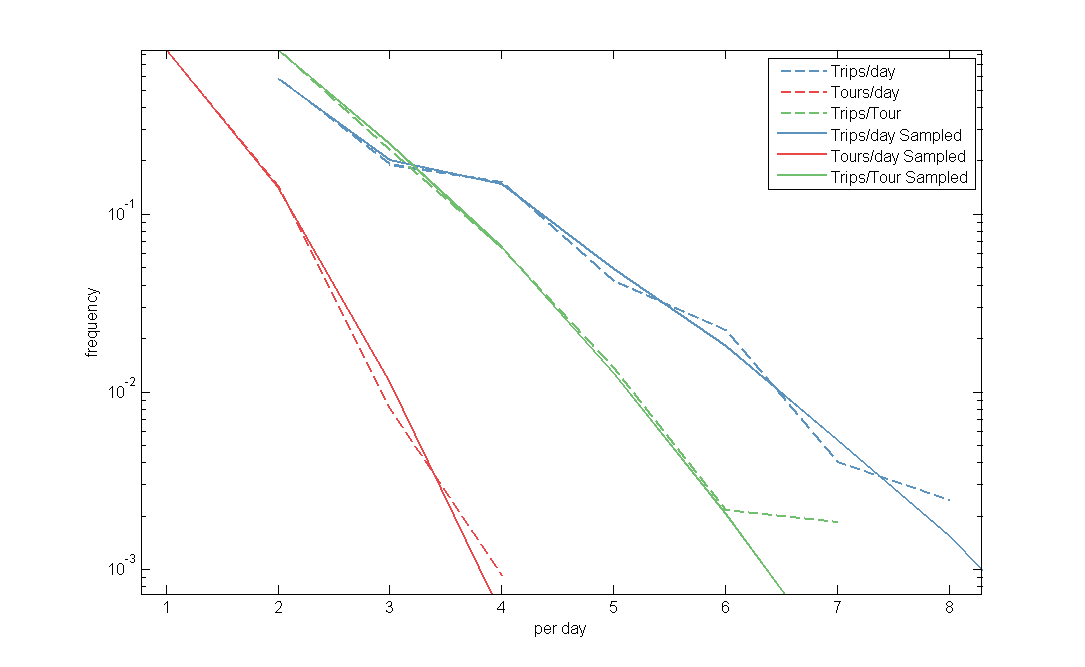
\includegraphics[width=\textwidth]{fig/LNToursPerDay.png}
%\caption{Distribution of number of trips, tours and trips per tour for simulated (solid) and real data (dashed). \label{fig:tours}}
%\end{figure}
\begin{figure}[b!]
%	% This file was created by matlab2tikz.
%
%The latest updates can be retrieved from
%  http://www.mathworks.com/matlabcentral/fileexchange/22022-matlab2tikz-matlab2tikz
%where you can also make suggestions and rate matlab2tikz.
%
\definecolor{mycolor1}{rgb}{0.34667,0.53600,0.69067}%
\definecolor{mycolor2}{rgb}{0.91529,0.28157,0.28784}%
\definecolor{mycolor3}{rgb}{0.44157,0.74902,0.43216}%
%
\begin{tikzpicture}

\begin{axis}[%
width=4.299in,
height=2.794in,
at={(0in,0in)},
scale only axis,
xmin=1,
xmax=9,
xlabel style={font=\footnotesize},
xlabel={\# per day},
ymode=log,
ymin=1e-06,
ymax=1,
yminorticks=true,
ylabel style={font=\footnotesize},
ylabel={frequency},
legend style={legend cell align=left, align=left},
legend pos = south west
]
\addplot [color=mycolor1, line width=1pt, mark=o, mark options={solid, mycolor1}]
  table[row sep=crcr]{%
2	0.6111\\
3	0.2021\\
4	0.1319\\
5	0.03848\\
6	0.01345\\
7	0.001121\\
8	0.0003736\\
};
\addlegendentry{Trips obs}

\addplot [color=mycolor1, dashed, line width=1pt, mark=x, mark options={solid, mycolor1}]
  table[row sep=crcr]{%
2	0.6105\\
3	0.1943\\
4	0.128\\
5	0.03754\\
6	0.0147\\
7	0.003676\\
8	0.001087\\
9	0.0002663\\
};
\addlegendentry{Trips sim}

\addplot [color=mycolor2, line width=1.0pt, mark=o, mark options={solid, mycolor2}]
  table[row sep=crcr]{%
1	0.8771\\
2	0.1177\\
3	0.004856\\
4	0.0003736\\
};
\addlegendentry{Tours obs}

\addplot [color=mycolor2, dashed, line width=1.0pt, mark=x, mark options={solid, mycolor2}]
  table[row sep=crcr]{%
1	0.8634\\
2	0.1168\\
3	0.009439\\
4	0.0004586\\
5	1.479e-05\\
};
\addlegendentry{Tours sim}

\addplot [color=mycolor3, line width=1.0pt, mark=o, mark options={solid, mycolor3}]
  table[row sep=crcr]{%
2	0.8252\\
3	0.2323\\
4	0.05491\\
5	0.01307\\
6	0.001121\\
7	0.0003736\\
};
\addlegendentry{Trips per tour obs}

\addplot [color=mycolor3, dashed, line width=1.0pt, mark=x, mark options={solid, mycolor3}]
  table[row sep=crcr]{%
2	0.8327\\
3	0.2287\\
4	0.05356\\
5	0.01047\\
6	0.001491\\
7	0.0002145\\
8	3.699e-05\\
9	3.699e-06\\
};
\addlegendentry{Trips per tour sim}

\end{axis}
\end{tikzpicture}%
	\caption{Distribution of number of trips, tours and trips per tour for simulated (dashed) and real data (solid). \label{fig:tours}}
\end{figure}

The length of trips by mode will mainly be determined by the utility of time and money for respectively mode and by network characteristics. This gives a good distribution of travel times, as can be seen in figure \ref{fig:triplength}. Since a large share of the trips are made to and from work, where the location is fixed and the trip is mandatory, the model is guaranteed to reproduce a large share of the trips well. However, the observed mode for the trip to work will only be the chosen mode in some of the simulated observations, and these restrictions will not give the distribution directly. 
%\begin{figure}[b!]
%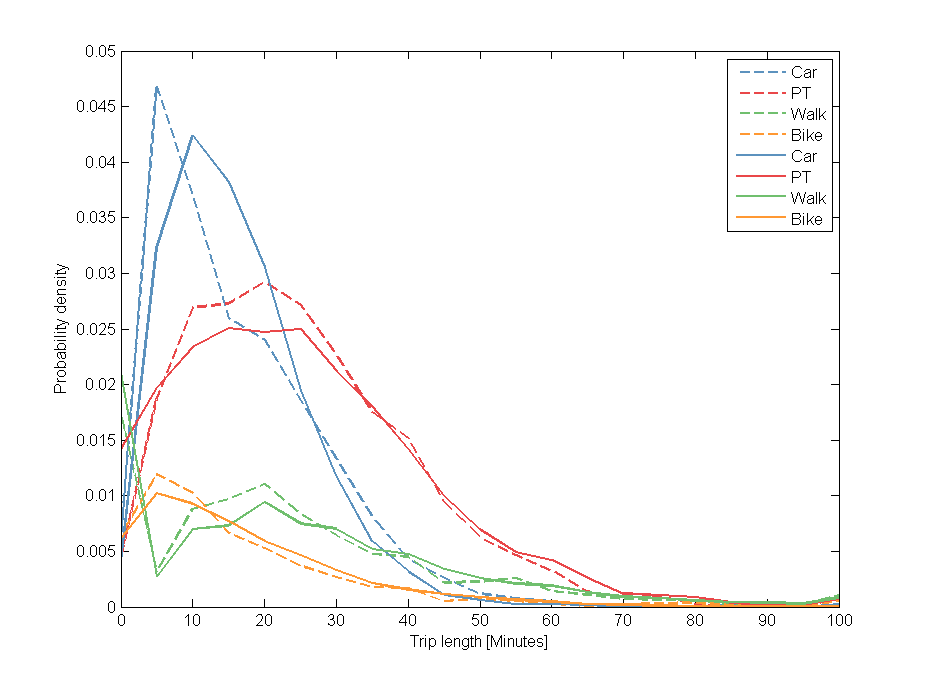
\includegraphics[width=\textwidth]{fig/TripLength.png}
%\caption{Distribution of trip lengths of respectively mode for simulated (solid) and real data (dashed). \label{fig:triplength}}
%\end{figure}
\begin{figure}[b!]
%	% This file was created by matlab2tikz.
%
%The latest updates can be retrieved from
%  http://www.mathworks.com/matlabcentral/fileexchange/22022-matlab2tikz-matlab2tikz
%where you can also make suggestions and rate matlab2tikz.
%
\definecolor{mycolor1}{rgb}{0.34667,0.53600,0.69067}%
\definecolor{mycolor2}{rgb}{0.91529,0.28157,0.28784}%
\definecolor{mycolor3}{rgb}{0.44157,0.74902,0.43216}%
\definecolor{mycolor4}{rgb}{1.00000,0.59843,0.20000}%
%
\begin{tikzpicture}

\begin{axis}[%
width=0.9\textwidth,
height=0.7\textwidth,
at={(0in,0in)},
scale only axis,
xmin=0,
xmax=80,
xlabel style={font=\footnotesize},
xlabel={Trip duration [minutes]},
ymin=0,
ymax=0.06,
ylabel style={font=\footnotesize},
ylabel={\#trips/\#individuals},
axis background/.style={fill=white},
axis x line*=bottom,
axis y line*=left,
legend style={legend cell align=left, align=left},
every axis plot/.append style = {very thick}
]
\addplot [color=mycolor1]
  table[row sep=crcr]{%
0	0\\
0.2	0.00131195335276968\\
0.6	0.00153061224489796\\
1.2	0.00233236151603499\\
2	0.00364431486880466\\
3	0.00663265306122449\\
4	0.00809037900874636\\
5	0.0115889212827988\\
6	0.0145043731778426\\
7	0.0169825072886297\\
8	0.0185860058309038\\
9	0.0206997084548105\\
10	0.0213556851311953\\
11	0.0228862973760933\\
12	0.0253644314868805\\
13	0.0267492711370262\\
14	0.027332361516035\\
15	0.0283527696793003\\
16	0.0283527696793003\\
17	0.0263848396501458\\
18	0.0247813411078717\\
19	0.0241253644314869\\
20	0.024198250728863\\
21	0.024198250728863\\
22	0.0270408163265306\\
23	0.0284985422740525\\
24	0.0287172011661808\\
25	0.0274052478134111\\
26	0.0276239067055394\\
27	0.0264577259475219\\
28	0.0259475218658892\\
29	0.025801749271137\\
30	0.0250728862973761\\
31	0.0243440233236152\\
32	0.0227405247813411\\
33	0.0219387755102041\\
34	0.0214285714285714\\
35	0.021064139941691\\
36	0.0200437317784257\\
37	0.0188775510204082\\
38	0.0180758017492711\\
39	0.0167638483965015\\
40	0.0167638483965015\\
41	0.0160349854227405\\
42	0.0156705539358601\\
43	0.0137755102040816\\
44	0.0129737609329446\\
45	0.0113702623906706\\
46	0.0100583090379009\\
47	0.00881924198250729\\
48	0.00845481049562682\\
49	0.00823615160349854\\
50	0.00772594752186589\\
51	0.00728862973760933\\
52	0.00670553935860058\\
53	0.00634110787172012\\
54	0.00517492711370262\\
55	0.00532069970845481\\
56	0.00488338192419825\\
57	0.00495626822157434\\
58	0.0043731778425656\\
59	0.00422740524781341\\
60	0.00400874635568513\\
61	0.00393586005830904\\
62	0.00335276967930029\\
63	0.00320699708454811\\
64	0.00269679300291545\\
65	0.00211370262390671\\
66	0.00145772594752187\\
67	0.0010932944606414\\
68	0.00087463556851312\\
69	0.000947521865889213\\
70	0.00087463556851312\\
71	0.00102040816326531\\
72	0.00087463556851312\\
73	0.00102040816326531\\
74	0.000801749271137026\\
75	0.00087463556851312\\
76	0.000801749271137026\\
77	0.000947521865889213\\
78	0.000728862973760933\\
79	0.00065597667638484\\
80	0.000510204081632653\\
81	0.00043731778425656\\
82	0.000291545189504373\\
83	0.00021865889212828\\
84	0.00021865889212828\\
85	7.28862973760933e-05\\
86	0\\
87	0\\
88	0\\
89	0.00021865889212828\\
90	0.000291545189504373\\
91	0.000291545189504373\\
92	0.000291545189504373\\
93	0.000291545189504373\\
94	7.28862973760933e-05\\
95	7.28862973760933e-05\\
96	7.28862973760933e-05\\
97	0.000145772594752187\\
98	0.000145772594752187\\
99	0.00021865889212828\\
100	0.000145772594752187\\
101	0.00021865889212828\\
102	0.000145772594752187\\
103	0.000145772594752187\\
104	7.28862973760933e-05\\
105	0.00021865889212828\\
106	0.00021865889212828\\
107	0.000291545189504373\\
108	0.000291545189504373\\
109	0.000291545189504373\\
110	0.000145772594752187\\
111	7.28862973760933e-05\\
112	7.28862973760933e-05\\
113	7.28862973760933e-05\\
114	7.28862973760933e-05\\
115	7.28862973760933e-05\\
116	7.28862973760933e-05\\
117	0.000291545189504373\\
};
\addlegendentry{PT - obs}

\addplot [color=mycolor1, dashed]
  table[row sep=crcr]{%
0	0\\
0.2	0.0073096452866861\\
0.6	0.00802028668610301\\
1.2	0.00950461613216715\\
2	0.0114696307094266\\
3	0.0144121720116618\\
4	0.0101766277939747\\
5	0.0128899416909621\\
6	0.0157780612244898\\
7	0.0182380952380952\\
8	0.0196468658892128\\
9	0.0211885325558795\\
10	0.0214658649173955\\
11	0.0217696793002915\\
12	0.0221224489795918\\
13	0.0227136783284742\\
14	0.0237849854227405\\
15	0.0245668124392614\\
16	0.0246864674441205\\
17	0.02447351797862\\
18	0.0242586248785228\\
19	0.0229341593780369\\
20	0.0233310252672498\\
21	0.0227930029154519\\
22	0.0235918367346939\\
23	0.0240817541302235\\
24	0.0244788629737609\\
25	0.0241831875607386\\
26	0.0251154033041788\\
27	0.025113824101069\\
28	0.0246537900874636\\
29	0.0240817541302235\\
30	0.0229539601554908\\
31	0.0222027453838678\\
32	0.0209515306122449\\
33	0.0203285957240039\\
34	0.0201310738581147\\
35	0.0200343780369291\\
36	0.0192509718172983\\
37	0.0183838678328474\\
38	0.0174444849368319\\
39	0.0162740524781341\\
40	0.0158284742468416\\
41	0.0145835762876579\\
42	0.0140313411078717\\
43	0.0131966715257532\\
44	0.0125810252672498\\
45	0.0111364188532556\\
46	0.0108101311953353\\
47	0.00994569970845481\\
48	0.00932009232264334\\
49	0.00893112244897959\\
50	0.00850911078717201\\
51	0.00759293002915452\\
52	0.00707689504373178\\
53	0.00653049076773566\\
54	0.00560835762876579\\
55	0.00565986394557823\\
56	0.00544144800777454\\
57	0.00508053935860058\\
58	0.00462585034013605\\
59	0.00465901360544218\\
60	0.00451737123420797\\
61	0.0042724732750243\\
62	0.00419059766763848\\
63	0.00427891156462585\\
64	0.00364965986394558\\
65	0.00336406705539359\\
66	0.00302113702623907\\
67	0.00254786200194363\\
68	0.0020205296404276\\
69	0.00197995626822157\\
70	0.00160119047619048\\
71	0.0015597667638484\\
72	0.00125291545189504\\
73	0.00119910106899903\\
74	0.00115974246841594\\
75	0.00114249271137026\\
76	0.000976190476190476\\
77	0.00104215257531584\\
78	0.00106584062196307\\
79	0.0010074101068999\\
80	0.00098153547133139\\
81	0.000959548104956268\\
82	0.000896137026239067\\
83	0.000712342079689018\\
84	0.000637998056365403\\
85	0.000524781341107872\\
86	0.000461491739552964\\
87	0.00038022351797862\\
88	0.000314261418853256\\
89	0.000260568513119533\\
90	0.000145408163265306\\
91	8.43051506316813e-05\\
92	0.000122084548104956\\
93	0.000125728862973761\\
94	9.99757045675413e-05\\
95	0.000124392614188533\\
96	0.000121234207968902\\
97	0.000137147716229349\\
98	0.000123177842565598\\
99	0.000157798833819242\\
100	0.000114795918367347\\
101	0.000176263362487852\\
102	0.000164601554907677\\
103	0.000162900874635569\\
104	0.000125242954324587\\
105	0.000284378036929057\\
106	0.000220724003887269\\
107	0.000193391642371234\\
108	0.000193999028182702\\
109	0.000193634596695821\\
110	3.31632653061225e-05\\
111	3.15840621963071e-05\\
112	2.28377065111759e-05\\
113	3.49854227405248e-05\\
114	3.60787172011662e-05\\
115	4.93197278911565e-05\\
116	4.95626822157434e-05\\
117	0.000177478134110787\\
};
\addlegendentry{PT - sim}

\addplot [color=mycolor2]
  table[row sep=crcr]{%
0	0\\
0.2	0.00721574344023324\\
0.6	0.00721574344023324\\
1.2	0.00721574344023324\\
2	0.0075801749271137\\
3	0.0133381924198251\\
4	0.014067055393586\\
5	0.0274052478134111\\
6	0.0381195335276968\\
7	0.0464285714285714\\
8	0.0501457725947522\\
9	0.0502915451895044\\
10	0.0440233236151603\\
11	0.0395043731778426\\
12	0.0370991253644315\\
13	0.0335276967930029\\
14	0.0317055393586006\\
15	0.0307580174927114\\
16	0.0294460641399417\\
17	0.0276239067055394\\
18	0.027332361516035\\
19	0.0259475218658892\\
20	0.0252915451895044\\
21	0.0251457725947522\\
22	0.0255830903790087\\
23	0.025\\
24	0.0235422740524781\\
25	0.0209183673469388\\
26	0.0204810495626822\\
27	0.0193877551020408\\
28	0.0171282798833819\\
29	0.0166909620991254\\
30	0.016399416909621\\
31	0.0147959183673469\\
32	0.0136297376093294\\
33	0.0137755102040816\\
34	0.0127551020408163\\
35	0.0113702623906706\\
36	0.0103498542274052\\
37	0.00911078717201166\\
38	0.00743440233236152\\
39	0.00634110787172012\\
40	0.00597667638483965\\
41	0.00553935860058309\\
42	0.00473760932944606\\
43	0.00408163265306122\\
44	0.00408163265306122\\
45	0.00379008746355685\\
46	0.00291545189504373\\
47	0.00262390670553936\\
48	0.00225947521865889\\
49	0.00174927113702624\\
50	0.00153061224489796\\
51	0.00160349854227405\\
52	0.00138483965014577\\
53	0.00145772594752187\\
54	0.00145772594752187\\
55	0.00131195335276968\\
56	0.00102040816326531\\
57	0.000947521865889213\\
58	0.000801749271137026\\
59	0.000583090379008746\\
60	0.000583090379008746\\
61	0.000510204081632653\\
62	0.000583090379008746\\
63	0.000583090379008746\\
64	0.000510204081632653\\
65	0.000364431486880466\\
66	0.000364431486880466\\
67	0.000291545189504373\\
68	0.000145772594752187\\
69	7.28862973760933e-05\\
70	7.28862973760933e-05\\
71	0\\
72	0\\
73	0\\
74	0\\
75	0\\
76	0\\
77	0\\
78	0\\
79	0\\
80	0\\
81	0\\
82	0\\
83	7.28862973760933e-05\\
84	7.28862973760933e-05\\
85	0.000145772594752187\\
86	0.000145772594752187\\
87	0.000145772594752187\\
88	7.28862973760933e-05\\
89	7.28862973760933e-05\\
90	0\\
91	0\\
92	0\\
93	0\\
94	0\\
95	0\\
96	0\\
97	0\\
98	0\\
99	0\\
100	0\\
101	0\\
102	0\\
103	0\\
104	0\\
105	0\\
106	0\\
107	7.28862973760933e-05\\
108	7.28862973760933e-05\\
109	7.28862973760933e-05\\
110	0.00021865889212828\\
111	0.00021865889212828\\
112	0.000145772594752187\\
113	0.000145772594752187\\
114	0.00021865889212828\\
115	7.28862973760933e-05\\
116	7.28862973760933e-05\\
117	7.28862973760933e-05\\
};
\addlegendentry{Car - obs}

\addplot [color=mycolor2, dashed]
  table[row sep=crcr]{%
0	0\\
0.2	0.00373955296404276\\
0.6	0.00373955296404276\\
1.2	0.00373955296404276\\
2	0.00415063168124393\\
3	0.00675898931000972\\
4	0.0090336491739553\\
5	0.0161873177842566\\
6	0.0249821428571429\\
7	0.0322192662779397\\
8	0.0388583576287658\\
9	0.0407502429543246\\
10	0.0423804664723032\\
11	0.0419165451895044\\
12	0.042405612244898\\
13	0.0406897473275024\\
14	0.0415481049562682\\
15	0.0410945092322643\\
16	0.0399249271137026\\
17	0.0393479105928086\\
18	0.0391806365403304\\
19	0.0366644800777454\\
20	0.0354769193391642\\
21	0.0345343780369291\\
22	0.0324653790087464\\
23	0.0298442662779397\\
24	0.0281673955296404\\
25	0.0251163751214772\\
26	0.0228910349854227\\
27	0.0210504130223518\\
28	0.019046768707483\\
29	0.0176540330417881\\
30	0.0158991739552964\\
31	0.0142706511175899\\
32	0.012700315840622\\
33	0.0119934402332362\\
34	0.0103111030126336\\
35	0.00909839650145773\\
36	0.00782543731778426\\
37	0.00667954324586978\\
38	0.0054365889212828\\
39	0.00462062682215743\\
40	0.00411880466472303\\
41	0.00362487852283771\\
42	0.00311115160349854\\
43	0.00258491253644315\\
44	0.00218974732750243\\
45	0.00175157920310982\\
46	0.00131584062196307\\
47	0.0011435860058309\\
48	0.00112585034013605\\
49	0.000939868804664723\\
50	0.00100413022351798\\
51	0.000895165208940719\\
52	0.000717930029154519\\
53	0.000621355685131195\\
54	0.000560009718172983\\
55	0.000335034013605442\\
56	0.000311224489795918\\
57	0.000295553935860058\\
58	0.000328960155490768\\
59	0.000295189504373178\\
60	0.000341472303206997\\
61	0.000315597667638484\\
62	0.000270165208940719\\
63	0.000160957240038873\\
64	0.00019290573372206\\
65	0.000162536443148688\\
66	0.000225340136054422\\
67	0.000217444120505345\\
68	0.000146622934888241\\
69	0.000111516034985423\\
70	7.27648202137998e-05\\
71	8.26044703595724e-06\\
72	8.86783284742468e-06\\
73	7.41010689990282e-06\\
74	7.16715257531584e-06\\
75	7.1064139941691e-05\\
76	0.000122691933916424\\
77	0.00012257045675413\\
78	0.000123299319727891\\
79	0.000124271137026239\\
80	6.07385811467444e-05\\
81	9.11078717201166e-06\\
82	7.28862973760933e-06\\
83	1.67638483965015e-05\\
84	1.56705539358601e-05\\
85	3.09766763848397e-05\\
86	2.93974732750243e-05\\
87	2.95189504373178e-05\\
88	1.84645286686103e-05\\
89	1.82215743440233e-05\\
90	2.30806608357629e-06\\
91	3.2798833819242e-06\\
92	3.15840621963071e-06\\
93	3.40136054421769e-06\\
94	3.40136054421769e-06\\
95	3.52283770651118e-06\\
96	2.55102040816327e-06\\
97	2.67249757045675e-06\\
98	2.91545189504373e-06\\
99	2.79397473275024e-06\\
100	2.55102040816327e-06\\
101	2.55102040816327e-06\\
102	2.30806608357629e-06\\
103	2.1865889212828e-06\\
104	2.55102040816327e-06\\
105	2.55102040816327e-06\\
106	2.1865889212828e-06\\
107	7.25218658892128e-05\\
108	7.22789115646259e-05\\
109	7.19144800777454e-05\\
110	7.17930029154519e-05\\
111	7.17930029154519e-05\\
112	8.50340136054422e-07\\
113	6.07385811467444e-07\\
114	4.62827988338192e-05\\
115	4.62827988338192e-05\\
116	4.65257531584062e-05\\
117	4.66472303206997e-05\\
};
\addlegendentry{Car - sim}

\addplot [color=mycolor3]
  table[row sep=crcr]{%
0	0\\
0.2	0.00233236151603499\\
0.6	0.00255102040816327\\
1.2	0.00466472303206997\\
2	0.00532069970845481\\
3	0.00714285714285714\\
4	0.00641399416909621\\
5	0.00823615160349854\\
6	0.00794460641399417\\
7	0.00940233236151604\\
8	0.00889212827988338\\
9	0.0086734693877551\\
10	0.00823615160349854\\
11	0.00845481049562682\\
12	0.00714285714285714\\
13	0.0064868804664723\\
14	0.00619533527696793\\
15	0.00612244897959184\\
16	0.0053935860058309\\
17	0.00553935860058309\\
18	0.00677842565597668\\
19	0.00685131195335277\\
20	0.00604956268221574\\
21	0.00561224489795918\\
22	0.0053935860058309\\
23	0.00415451895043732\\
24	0.00451895043731778\\
25	0.0043731778425656\\
26	0.00451895043731778\\
27	0.00422740524781341\\
28	0.00415451895043732\\
29	0.00291545189504373\\
30	0.00291545189504373\\
31	0.0021865889212828\\
32	0.00269679300291545\\
33	0.00255102040816327\\
34	0.00276967930029155\\
35	0.00262390670553936\\
36	0.00284256559766764\\
37	0.00196793002915452\\
38	0.00189504373177843\\
39	0.00167638483965015\\
40	0.00174927113702624\\
41	0.00160349854227405\\
42	0.00182215743440233\\
43	0.00153061224489796\\
44	0.00123906705539359\\
45	0.00102040816326531\\
46	0.00087463556851312\\
47	0.000728862973760933\\
48	0.00065597667638484\\
49	0.00087463556851312\\
50	0.000583090379008746\\
51	0.00065597667638484\\
52	0.000728862973760933\\
53	0.000801749271137026\\
54	0.00087463556851312\\
55	0.00102040816326531\\
56	0.000801749271137026\\
57	0.00065597667638484\\
58	0.00065597667638484\\
59	0.000364431486880466\\
60	0.00021865889212828\\
61	0.00043731778425656\\
62	0.000364431486880466\\
63	0.00043731778425656\\
64	0.00043731778425656\\
65	0.00043731778425656\\
66	0.000145772594752187\\
67	0.000145772594752187\\
68	0.000145772594752187\\
69	0.000145772594752187\\
70	0.00021865889212828\\
71	0.00021865889212828\\
72	0.000291545189504373\\
73	0.000291545189504373\\
74	0.00043731778425656\\
75	0.000364431486880466\\
76	0.00043731778425656\\
77	0.000364431486880466\\
78	0.000291545189504373\\
79	0.00021865889212828\\
80	0.000364431486880466\\
81	0.000364431486880466\\
82	0.00043731778425656\\
83	0.00043731778425656\\
84	0.00043731778425656\\
85	0.000291545189504373\\
86	0.00021865889212828\\
87	0.000145772594752187\\
88	7.28862973760933e-05\\
89	0\\
90	0\\
91	7.28862973760933e-05\\
92	7.28862973760933e-05\\
93	7.28862973760933e-05\\
94	7.28862973760933e-05\\
95	0.000145772594752187\\
96	0.000145772594752187\\
97	0.000145772594752187\\
98	0.000145772594752187\\
99	0.000145772594752187\\
100	7.28862973760933e-05\\
101	0.000145772594752187\\
102	0.000145772594752187\\
103	0.000145772594752187\\
104	0.000145772594752187\\
105	0.000145772594752187\\
106	0\\
107	0\\
108	0\\
109	0\\
110	0\\
111	0\\
112	0\\
113	0\\
114	7.28862973760933e-05\\
115	7.28862973760933e-05\\
116	0.000145772594752187\\
117	0.000291545189504373\\
};
\addlegendentry{Bike - obs}

\addplot [color=mycolor3, dashed]
  table[row sep=crcr]{%
0	0\\
0.2	0.00207956754130224\\
0.6	0.00248226433430515\\
1.2	0.00336601068999028\\
2	0.00443221574344023\\
3	0.00568500971817298\\
4	0.00532774538386783\\
5	0.00639504373177842\\
6	0.00741715257531584\\
7	0.00814224975704568\\
8	0.00843598153547133\\
9	0.00837779397473275\\
10	0.00856499028182702\\
11	0.00820347424684159\\
12	0.00791569484936832\\
13	0.00769484936831876\\
14	0.00770833333333333\\
15	0.00745201652089407\\
16	0.00735993683187561\\
17	0.00706972789115646\\
18	0.0071082361516035\\
19	0.00661321671525753\\
20	0.00616375121477162\\
21	0.00578765792031098\\
22	0.00560519922254616\\
23	0.0052463556851312\\
24	0.00512390670553936\\
25	0.00505478620019436\\
26	0.00491277939747327\\
27	0.00464067055393586\\
28	0.00450218658892128\\
29	0.00410131195335277\\
30	0.00375874635568513\\
31	0.00345505344995141\\
32	0.00334900388726919\\
33	0.00297120991253644\\
34	0.00283442662779397\\
35	0.00265415451895044\\
36	0.00252223032069971\\
37	0.00232847424684159\\
38	0.00216885325558795\\
39	0.00208466958211856\\
40	0.00199829931972789\\
41	0.00179968415937804\\
42	0.00163751214771623\\
43	0.00157932458697765\\
44	0.00138168124392614\\
45	0.00133345481049563\\
46	0.0012593537414966\\
47	0.00120177356656948\\
48	0.0011064139941691\\
49	0.00107810981535471\\
50	0.00105988824101069\\
51	0.000980320699708455\\
52	0.000900267249757046\\
53	0.000871355685131195\\
54	0.0008283527696793\\
55	0.000765427599611273\\
56	0.000780369290573372\\
57	0.000755952380952381\\
58	0.000725704567541302\\
59	0.000665087463556851\\
60	0.00060653547133139\\
61	0.000552478134110787\\
62	0.000503158406219631\\
63	0.000468901846452867\\
64	0.00040913508260447\\
65	0.00039067055393586\\
66	0.000331875607385811\\
67	0.000292031098153547\\
68	0.000266156462585034\\
69	0.00026044703595724\\
70	0.000246720116618076\\
71	0.000253279883381924\\
72	0.000247327502429543\\
73	0.000223275024295432\\
74	0.000205903790087464\\
75	0.000170918367346939\\
76	0.000139941690962099\\
77	0.000119290573372206\\
78	0.000105442176870748\\
79	0.000100826044703596\\
80	0.000105442176870748\\
81	9.96112730806608e-05\\
82	9.29300291545189e-05\\
83	9.03790087463557e-05\\
84	8.50340136054422e-05\\
85	7.39795918367347e-05\\
86	7.17930029154519e-05\\
87	6.81486880466472e-05\\
88	5.988824101069e-05\\
89	5.64868804664723e-05\\
90	5.24781341107872e-05\\
91	4.49465500485909e-05\\
92	4.3245869776482e-05\\
93	4.08163265306122e-05\\
94	3.42565597667639e-05\\
95	3.13411078717201e-05\\
96	2.90330417881438e-05\\
97	2.86686103012634e-05\\
98	3.04907677356657e-05\\
99	3.02478134110787e-05\\
100	2.80612244897959e-05\\
101	2.59961127308066e-05\\
102	2.34450923226433e-05\\
103	1.78571428571429e-05\\
104	1.49416909620991e-05\\
105	1.57920310981535e-05\\
106	1.50631681243926e-05\\
107	1.22691933916424e-05\\
108	1.16618075801749e-05\\
109	9.83965014577259e-06\\
110	8.38192419825073e-06\\
111	7.04567541302235e-06\\
112	6.80272108843537e-06\\
113	5.95238095238095e-06\\
114	5.83090379008746e-06\\
115	6.31681243926142e-06\\
116	4.73760932944606e-06\\
117	2.52672497570457e-05\\
};
\addlegendentry{Bike - sim}

\addplot [color=mycolor4]
  table[row sep=crcr]{%
0	0\\
0.2	0.0129008746355685\\
0.6	0.0129008746355685\\
1.2	0.0129008746355685\\
2	0.0129008746355685\\
3	0.0129737609329446\\
4	0.00043731778425656\\
5	0.00131195335276968\\
6	0.00189504373177843\\
7	0.00306122448979592\\
8	0.00400874635568513\\
9	0.00495626822157434\\
10	0.00502915451895044\\
11	0.00590379008746356\\
12	0.00619533527696793\\
13	0.00619533527696793\\
14	0.00685131195335277\\
15	0.00685131195335277\\
16	0.00736151603498542\\
17	0.00743440233236152\\
18	0.00728862973760933\\
19	0.00750728862973761\\
20	0.00816326530612245\\
21	0.0076530612244898\\
22	0.00779883381924198\\
23	0.00838192419825073\\
24	0.00794460641399417\\
25	0.00721574344023324\\
26	0.0065597667638484\\
27	0.00685131195335277\\
28	0.00677842565597668\\
29	0.00612244897959184\\
30	0.00699708454810496\\
31	0.00721574344023324\\
32	0.00597667638483965\\
33	0.00561224489795918\\
34	0.00502915451895044\\
35	0.00400874635568513\\
36	0.00400874635568513\\
37	0.00430029154518951\\
38	0.00422740524781341\\
39	0.00473760932944606\\
40	0.00481049562682216\\
41	0.00444606413994169\\
42	0.00430029154518951\\
43	0.00379008746355685\\
44	0.00335276967930029\\
45	0.00291545189504373\\
46	0.00247813411078717\\
47	0.00182215743440233\\
48	0.00153061224489796\\
49	0.00116618075801749\\
50	0.00102040816326531\\
51	0.00153061224489796\\
52	0.00167638483965015\\
53	0.00189504373177843\\
54	0.00204081632653061\\
55	0.00240524781341108\\
56	0.0021865889212828\\
57	0.00225947521865889\\
58	0.0021865889212828\\
59	0.00211370262390671\\
60	0.00182215743440233\\
61	0.00153061224489796\\
62	0.00138483965014577\\
63	0.00123906705539359\\
64	0.00116618075801749\\
65	0.00123906705539359\\
66	0.00116618075801749\\
67	0.00123906705539359\\
68	0.00131195335276968\\
69	0.00123906705539359\\
70	0.00087463556851312\\
71	0.000728862973760933\\
72	0.000801749271137026\\
73	0.000801749271137026\\
74	0.000801749271137026\\
75	0.00087463556851312\\
76	0.00087463556851312\\
77	0.000510204081632653\\
78	0.000291545189504373\\
79	0.000291545189504373\\
80	0.00043731778425656\\
81	0.000510204081632653\\
82	0.00043731778425656\\
83	0.000510204081632653\\
84	0.000364431486880466\\
85	0.000145772594752187\\
86	0.000145772594752187\\
87	0.000291545189504373\\
88	0.00021865889212828\\
89	0.00021865889212828\\
90	0.000364431486880466\\
91	0.000291545189504373\\
92	0.000145772594752187\\
93	0.000291545189504373\\
94	0.000291545189504373\\
95	0.000145772594752187\\
96	0.000145772594752187\\
97	0.000145772594752187\\
98	0\\
99	7.28862973760933e-05\\
100	7.28862973760933e-05\\
101	0.000145772594752187\\
102	0.000145772594752187\\
103	0.000145772594752187\\
104	7.28862973760933e-05\\
105	7.28862973760933e-05\\
106	0\\
107	7.28862973760933e-05\\
108	7.28862973760933e-05\\
109	0.000145772594752187\\
110	0.000145772594752187\\
111	0.00021865889212828\\
112	0.000145772594752187\\
113	0.00021865889212828\\
114	0.00021865889212828\\
115	0.00021865889212828\\
116	0.00021865889212828\\
117	0.00043731778425656\\
};
\addlegendentry{Walk - obs}

\addplot [color=mycolor4, dashed]
  table[row sep=crcr]{%
0	0\\
0.2	0.0130970602526725\\
0.6	0.0131183187560739\\
1.2	0.0131437074829932\\
2	0.0132995626822157\\
3	0.0134716958211856\\
4	0.000732871720116618\\
5	0.00143488824101069\\
6	0.00216836734693878\\
7	0.00282240038872692\\
8	0.00351882896015549\\
9	0.00453194849368319\\
10	0.00524611273080661\\
11	0.00560532069970845\\
12	0.00630660835762877\\
13	0.00642857142857143\\
14	0.00658053935860058\\
15	0.00663216715257532\\
16	0.00708199708454811\\
17	0.00669557823129252\\
18	0.00711831875607386\\
19	0.00698821671525753\\
20	0.00715585519922255\\
21	0.00744071914480078\\
22	0.0079758260447036\\
23	0.00816010689990282\\
24	0.00799125364431487\\
25	0.00747776967930029\\
26	0.00687840136054422\\
27	0.00652162293488824\\
28	0.00620262390670554\\
29	0.00631778425655977\\
30	0.00641253644314869\\
31	0.00637815840621963\\
32	0.00597509718172983\\
33	0.00578510689990282\\
34	0.00527174441205053\\
35	0.00497971331389699\\
36	0.00451530612244898\\
37	0.00439698736637512\\
38	0.00400036443148688\\
39	0.00397120991253644\\
40	0.00362159863945578\\
41	0.00370201652089407\\
42	0.00360495626822157\\
43	0.00344448493683188\\
44	0.00331073858114674\\
45	0.00334463070942663\\
46	0.00299854227405248\\
47	0.00286771137026239\\
48	0.00272278911564626\\
49	0.00259961127308066\\
50	0.00239249271137026\\
51	0.00242674927113703\\
52	0.00224562682215743\\
53	0.00222303206997085\\
54	0.00197096695821186\\
55	0.00184851797862002\\
56	0.00159657434402332\\
57	0.0014608843537415\\
58	0.00149744897959184\\
59	0.0015\\
60	0.00151797862001944\\
61	0.00150801749271137\\
62	0.00153838678328474\\
63	0.00129907677356657\\
64	0.00121404275996113\\
65	0.00117334791059281\\
66	0.00109183673469388\\
67	0.00101214771622935\\
68	0.00103705053449951\\
69	0.00100983965014577\\
70	0.000856778425655977\\
71	0.000812074829931973\\
72	0.000747934888241011\\
73	0.000707240038872692\\
74	0.000706146744412051\\
75	0.000678206997084548\\
76	0.000715621963070943\\
77	0.000711856171039844\\
78	0.000654033041788144\\
79	0.000579567541302235\\
80	0.000580539358600583\\
81	0.000470359572400389\\
82	0.000430636540330418\\
83	0.000436588921282799\\
84	0.000416545189504373\\
85	0.000381559766763848\\
86	0.000393221574344023\\
87	0.000379494655004859\\
88	0.000348760932944606\\
89	0.000315233236151603\\
90	0.000316933916423712\\
91	0.000294460641399417\\
92	0.000262512147716229\\
93	0.000251700680272109\\
94	0.000250121477162293\\
95	0.000239431486880466\\
96	0.000236030126336249\\
97	0.000239067055393586\\
98	0.000221817298347911\\
99	0.000207968901846453\\
100	0.00017930029154519\\
101	0.000171282798833819\\
102	0.00016435860058309\\
103	0.000157191448007775\\
104	0.000158041788143829\\
105	0.00016120019436346\\
106	0.000143586005830904\\
107	0.000143586005830904\\
108	0.00013301749271137\\
109	0.00011698250728863\\
110	0.000110422740524781\\
111	0.000109936831875607\\
112	9.7667638483965e-05\\
113	9.63313896987366e-05\\
114	9.17152575315841e-05\\
115	9.05004859086492e-05\\
116	8.33333333333333e-05\\
117	0.000316083576287658\\
};
\addlegendentry{Walk - sim}

\end{axis}
\end{tikzpicture}%
	\caption{Distribution of trip lengths of respectively mode for observed choices (solid) and simulated (dashed). The plot has been obtained by first constructing a histogram with bin-size of one minute, and then average each time step over the closest 5 minutes. \label{fig:triplength}}
\end{figure}
 
% To do- also plot activity duration



The ``same zone'' dummy parameter $\param{s.z, walk}$ for walk is negative, which seems contra-intuitive as one would expect walk to be the preferred mode of transport for shorter distances. From figure \ref{fig:triplength} it is clear that for same-zone trips (trips with zero travel time) walk is still the preferred mode of transport. The reason for this is that the mode specific constant $\param{walk}$ is the largest of the constants, even after adding $\param{s.z, walk}$, and when the travel time is small it will therefore have the highest utility.

The parameters for travel time are almost the same for car, walk and bike but significantly smaller for PT. Since the travel time is longer for bike and walk, they will be less common for longer trips. PT has the smallest time coefficient and trips with longer travel time are therefore more common with public transport. The lower speed of bike and walk in comparison with the motorised modes will make them less common for longer trips, as can be seen in figure \ref{fig:triplength}. The lower alternative specific constants, and the fact that more locations will become available with the same travel time with PT and car also make bike and walk less common.




\FloatBarrier

\section{Discussion}
\subsection{To add}

We currently have linear-


\subsection{Correlation between alternatives}
It is common practice in route choice modelling to add a size attribute to each link to take correlation among paths that overlap into account, e.g., using Path-Size Logit \citep{BenAkivaBier99}. For their link-based route choice model, \citet{fosgerau11} obtains a size coefficient by calculating \eutil\, in each link using some pre-specified parameters and adding that to the link-utility. In the activity-scheduling model presented here, it is not as easy to define the overlapping of paths, as the network is dynamic. If two paths are identical besides that the start time for all activities in one path is $10\unit{min}$ after the start time in the other path, there can be practically no overlapping as defined by the Path-Size Logit although the two paths would be very similar. How to address this issue in a dynamic network and in the activity-scheduling framework is therefore an open question.

In trip-generation models, it is common to have nests for mode choice, location choice and activity choice, as in, e.g., \citet{Bowman01}. It would be possible to introduce different scales for the error term when solving \refeq{eq:EV} and obtaining choice probabilities in \refeq{eq:MNL} where the scale (which is one here) would be state dependent. This is done in the Nested Recursive Logit model described in \citet{mai2015}. However, the probability of a path would then not reduce to  \refeq{eq:pPath} and sampling of alternative sequences would not be possible to use for estimation.
\citet{guevara2013MEV} recently showed that Multivariate Extreme Value (MEV) models such as Nested Logit can be estimated using sampling of alternatives. A Nested RL-model is however not the same as an MEV model, so the transferability of the result is uncertain. If nests are introduced within the network, as in \citet{mai2015}, it would further require that the value function was approximated in all states, so the computational benefit might not be enough. An alternative would be to introduce nests over paths, for example nesting alternatives that include specific activities or modes. This would move the model in the direction of \citet{Bowman01}. The computation time is however likely to grow linearly with the number of nests. Given that the model already is time demanding, creating nests for all combinations of modes and activities would not be computationally feasible.

 Another issue is the correlation in preferences over time. Individuals' variances in preferences for, e.g., mode or activities are likely to be consistent over time and therefore to some extent be the same throughout the day. Including nests on a trip level would not capture this correlation. A possible solution would be to introduce mixed parameters for, e.g., activities and modes, that would be the same for each individual for the full day. Our estimation approach is based on sampling of alternatives and recent research by \citet{Guevara13} shows that the same method gives consistent estimates for mixed logit models. This has been explored in an extension of the work presented here in \citep{maelleMixed17}.

Finally, it is worth noting that the expected value function in \refeq{eq:MNL} might pick up some of the correlation in the unobservable $\epsilon$ that is usually captured by introducing nests in a trip or tour based model. Since a trip with walk, public transport and bike all share the same state, except for the arrival time, \eutil will be correlated for the three alternatives.
\section{Conclusions}
During the last decades, many activity-based models have been developed in the literature. However, there is still a lack of random-utility based models for which time integrates consistently in all choice dimensions. A natural approach would be to introduce time explicitly in the models, respecting that time has a direction and that it is possible to make decisions sequentially taking into account the available information at that time. It is also natural to respect that people are not completely myopic, but are capable of forward--looking, for instance taking into account the consequences for afternoon activity opportunities when deciding whether to take the car to work in the morning. 

The challenge with such a natural extension of the existing state-of-practice modelling framework is the immense combinatorial problem of, at least technically and consistently, considering all possible combinations of activity-location pattern throughout one single day, let alone combinations of days. In this paper, we formulate a dynamic discrete choice model which overcomes this curse of dimensionality using dynamic programming. In the framework, time is respected in the above-mentioned aspects making it dynamically consistent. 
We also demonstrate that it is indeed possible to estimate the model. Estimation is the main purpose and the main achievement of this paper. The proposed and thus estimated model is also validated in-sample. 

There are a number of immediate extensions of this model that can and will be explored in further research. First, it is natural to extend the model to multiple days. Some activities can be postponed to later days, and there is interaction between activity patterns during consecutive days. For instance, shopping for food is an activity in which a planning horizon of more than one day is very relevant to consider. 

Another limitation of the model proposed in this paper is the IID assumption between daily activity schedules. In a sequential decision context, it may be important to consider fixed effects, in particular recognizing that the same individual is making the decisions throughout one day. A natural extension of this model is therefore to consider a mixed panel logit model, where preferences for, e.g., cost, time, modes and activities are heterogeneous between individuals but constant throughout the day for a single individual.

The main challenge addressed in this paper was consistent estimation. This has hindered the use of such models in the past. Another very important aspect is to operationalize the model in implementation. For instance, when using the proposed model in the context of (or in conjunction with) a Dynamic Traffic Assignment (DTA) model, it will be necessary to repeatedly simulate travel schedules for millions of individuals. The naive approach would be to first calculate the value function in all states for each individual, but with the current specifications this would be prohibitively time consuming. Methods to speed up this simulation must therefore be developed.

\section*{Acknowledgments}
The work was conducted with financial support from the Centre for Transport Studies, Royal Institute of Technology, Sweden. The computations were performed on resources provided by the Swedish National Infrastructure for Computing (SNIC) at the National Supercomputer Centre at Link\"oping University (NSC). Earlier versions of this paper has been presented at the Transportation Research Board 93rd Annual Meeting (2014), at IRUC seminars at DTU (2014,2015) and at the Workshop on Discrete Choice Models at EPFL (2013). The work presented in this paper has greatly benefited from comments received from the participants of these conferences and workshops.

\footnotesize
\bibliographystyle{apalike}
\bibliography{transport,transport2,kappa,car,mixed}
%\bibliographystyle{plain}

%\bibliographystyle{../ref/apalike-doi}
\end{document} 
